\documentclass[twoside,11pt,fleqn]{book}

\usepackage[switch*,pagewise]{lineno}
\usepackage[dvipdfmx]{graphicx}
\usepackage[dvipdfmx]{color}

\usepackage{titlesec}
\setcounter{secnumdepth}{4}

\usepackage[nottoc,notlot,notlof]{tocbibind}

\usepackage[framemethod=TikZ]{mdframed}
\newmdenv[%
backgroundcolor=red!8,
linecolor=red,
outerlinewidth=1pt,
%roundcorner=5mm,
skipabove=\baselineskip,
skipbelow=\baselineskip,
]{mdbox}

\usepackage[dvipdfmx]{hyperref}
\usepackage{pxjahyper}
\hypersetup{colorlinks, citecolor=black, filecolor=black, linkcolor=blue, urlcolor=black}
%\usepackage{bookmark}

\usepackage[toc,nonumberlist]{glossaries}

%\usepackage{floatrow}
%\floatsetup[table]{capposition=top}
%\newfloatcommand{capbtabbox}{table}[][\FBwidth]

\usepackage{array}
\newcolumntype{L}[1]{>{\raggedright\let\newline\\\arraybackslash\hspace{0pt}}m{#1}}
\newcolumntype{C}[1]{>{\centering\let\newline\\\arraybackslash\hspace{0pt}}m{#1}}
\newcolumntype{R}[1]{>{\raggedleft\let\newline\\\arraybackslash\hspace{0pt}}m{#1}}
\usepackage{amssymb}

\usepackage{placeins}
\usepackage{multirow}
\usepackage[toc,page]{appendix}
\usepackage{fancyvrb}
\usepackage{xcolor}
\usepackage{listings}
\usepackage{url}
\usepackage[normalem]{ulem}
\usepackage{soul}
\DeclareRobustCommand{\hsout}[1]{\texorpdfstring{\sout{#1}}{#1}}

\usepackage{amsmath}
\usepackage{epic}
\usepackage{eepic}

\newcommand\textttw[1]{\mathchardef\UrlBreakPenalty=100\mathchardef\UrlBigBreakPenalty=100\url{#1}}
%%%%%%%%%%%%%%%%%%%%%%%%%%%%%%%%%%%%%%%%%%%%%%%%%%%%%%
% Define a new command \subsubsubsection
\titleclass{\subsubsubsection}{straight}[\subsection]

\newcounter{subsubsubsection}[subsubsection]
\renewcommand\thesubsubsubsection{\thesubsubsection.\arabic{subsubsubsection}}
\renewcommand\theparagraph{\thesubsubsubsection.\arabic{paragraph}} % optional; useful if paragraphs are to be numbered

\titleformat{\subsubsubsection}
  {\normalfont\normalsize\bfseries}{\thesubsubsubsection}{1em}{}
\titlespacing*{\subsubsubsection}
{0pt}{3.25ex plus 1ex minus .2ex}{1.5ex plus .2ex}

\makeatletter
\renewcommand\paragraph{\@startsection{paragraph}{5}{\z@}%
  {3.25ex \@plus1ex \@minus.2ex}%
  {-1em}%
  {\normalfont\normalsize\bfseries}}
\renewcommand\subparagraph{\@startsection{subparagraph}{6}{\parindent}%
  {3.25ex \@plus1ex \@minus .2ex}%
  {-1em}%
  {\normalfont\normalsize\bfseries}}
\def\toclevel@subsubsubsection{4}
\def\toclevel@paragraph{5}
\def\toclevel@paragraph{6}
\def\l@subsubsubsection{\@dottedtocline{4}{7em}{4em}}
\def\l@paragraph{\@dottedtocline{5}{10em}{5em}}
\def\l@subparagraph{\@dottedtocline{6}{14em}{6em}}
\makeatother
%%%%%%%%%%%%%%%%%%%%%%%%%%%%%%%%%%%%%%%%%%%%%%%%%%%%%%
\long\def\comment#1{}

\usepackage{etoolbox}
\usepackage{datetime}

\DefineVerbatimEnvironment{VerbX}{Verbatim}{}

\newenvironment{myverbt}
  {\VerbatimEnvironment
   \par\VerbX}
  {\endVerbX }

\newenvironment{myverbf}
  {\VerbatimEnvironment
   \par\vspace{\dimexpr-1.2\baselineskip\relax}
   \VerbX}
  {\endVerbX }

%   \par\vspace{\dimexpr-1.2\topsep-1.2\partopsep\relax}

% WG合意内容からの差異を赤字で表示
\ifx \HLDIFFWG y
\long\def\DIFFWG#1{\textcolor{red}{#1}}
\else
\long\def\DIFFWG#1{#1}
\fi

% 2017/7/21版と2017/7/31版の差異を赤字で表示
\ifx \HLDIFFJULTWO y
\long\def\ADDJULTWO#1{\textcolor{red}{#1}}
\long\def\MODJULTWO#1{\textcolor{red}{#1}}
\long\def\RMJULTWO#1{\textcolor{red}{\hsout{#1}}}
\long\def\ADDJULTWOS#1{\textcolor{red}{【追加】#1}}
\long\def\MODJULTWOS#1{\textcolor{red}{【変更】#1}}
\long\def\RMJULTWOS#1{\textcolor{red}{【削除】#1}}
\else
\long\def\ADDJULTWO#1{#1}
\long\def\MODJULTWO#1{#1}
\long\def\RMJULTWO#1{}
\long\def\ADDJULTWOS#1{#1}
\long\def\MODJULTWOS#1{#1}
\long\def\RMJULTWOS#1{#1}
\fi

% 2017/7/31版と2017/8/31版の差異を赤字で表示
\ifx \HLDIFFAUG y
\long\def\ADDAUG#1{\textcolor{red}{#1}}
\long\def\MODAUG#1{\textcolor{red}{#1}}
\long\def\RMAUG#1{\textcolor{red}{\hsout{#1}}}
\long\def\ADDAUGS#1{\textcolor{red}{【追加】#1}}
\long\def\MODAUGS#1{\textcolor{red}{【変更】#1}}
\long\def\RMAUGS#1{\textcolor{red}{【削除】#1}}
\else
\long\def\ADDAUG#1{#1}
\long\def\MODAUG#1{#1}
\long\def\RMAUG#1{}
\long\def\ADDAUGS#1{#1}
\long\def\MODAUGS#1{#1}
\long\def\RMAUGS#1{#1}
\fi

% V1.2.6とV1.2.7の差異(V1.3.0とV1.3.1の差異)を赤字で表示
\ifx \HLDIFFSEP y
\long\def\ADDSEP#1{\textcolor{red}{#1}}
\long\def\MODSEP#1{\textcolor{red}{#1}}
\long\def\RMSEP#1{\textcolor{red}{\hsout{#1}}}
\long\def\ADDSEPS#1{\textcolor{red}{【追加】#1}}
\long\def\MODSEPS#1{\textcolor{red}{【変更】#1}}
\long\def\RMSEPS#1{\textcolor{red}{【削除】#1}}
\else
\long\def\ADDSEP#1{#1}
\long\def\MODSEP#1{#1}
\long\def\RMSEP#1{}
\long\def\ADDSEPS#1{#1}
\long\def\MODSEPS#1{#1}
\long\def\RMSEPS#1{#1}
\fi

% 1.4.0からの差異を赤字で表示
\ifx \HLDIFFMAR y
\long\def\ADDMAR#1{\textcolor{red}{#1}}
\long\def\MODMAR#1{\textcolor{red}{#1}}
\long\def\RMMAR#1{\textcolor{red}{\hsout{#1}}}
\long\def\ADDMARS#1{\textcolor{red}{【追加】#1}}
\long\def\MODMARS#1{\textcolor{red}{【変更】#1}}
\long\def\RMMARS#1{\textcolor{red}{【削除】#1}}
\else
\long\def\ADDMAR#1{#1}
\long\def\MODMAR#1{#1}
\long\def\RMMAR#1{}
\long\def\ADDMARS#1{#1}
\long\def\MODMARS#1{#1}
\long\def\RMMARS#1{#1}
\fi

% 一つ前のバージョンとの差異を赤字で表示
\ifx \HLDIFFPREV y
\long\def\ADDPREV#1{\textcolor{red}{#1}}
\long\def\MODPREV#1{\textcolor{red}{#1}}
\long\def\RMPREV#1{\textcolor{red}{\hsout{#1}}}
\long\def\ADDPREVS#1{\textcolor{red}{【追加】#1}}
\long\def\MODPREVS#1{\textcolor{red}{【変更】#1}}
\long\def\RMPREVS#1{\textcolor{red}{【削除】#1}}
\else
\long\def\ADDPREV#1{#1}
\long\def\MODPREV#1{#1}
\long\def\RMPREV#1{}
\long\def\ADDPREVS#1{#1}
\long\def\MODPREVS#1{#1}
\long\def\RMPREVS#1{#1}
\fi

% diff rc3 rc4
\ifx \HLDIFFRCF y
\long\def\ADDRCF#1{\textcolor{red}{#1}}
\long\def\MODRCF#1{\textcolor{red}{#1}}
\long\def\RMRCF#1{\textcolor{red}{\hsout{#1}}}
\long\def\ADDRCFS#1{\textcolor{red}{【追加】#1}}
\long\def\MODRCFS#1{\textcolor{red}{【変更】#1}}
\long\def\RMRCFS#1{\textcolor{red}{【削除】#1}}
\else
\long\def\ADDRCF#1{#1}
\long\def\MODRCF#1{#1}
\long\def\RMRCF#1{}
\long\def\ADDRCFS#1{#1}
\long\def\MODRCFS#1{#1}
\long\def\RMRCFS#1{#1}
\fi

\pagestyle{plain}
\setcounter{tocdepth}{3}
\marginparwidth 0pt
\oddsidemargin=.25in
\evensidemargin  .25in
\marginparsep 0pt
\topmargin=-.5in
\textwidth=6.0in
\textheight=9.0in
\parindent=2em

% \chapter{Terms}
% 本章では用語とその定義を説明する。
% \begin{description}
\newglossaryentry{レイテンシコア}{name=レイテンシコア, description={シングルスレッド実行における遅延削減に重点を置いて開発されたプロセッサのコア。}}
%または結果が出始めるまでのコストであるスタートアップコストを小さくすることに重点を置いて開発されたプロセッサのコア。
\newglossaryentry{ノード}{name=ノード, description={一つ以上のプロセッサ、それらに接続されたRAM、それらに接続されたI/Oデバイスから構成されるコンピュータで、スーパーコンピュータはこれらの群で構成される。}}
\newglossaryentry{OSサービス}{name=OSサービス, description={プロセス管理、メモリ管理、システムコールなどアプリケーションに提供するハードウェア仮想化サービス。}}
\newglossaryentry{汎用OS}{name=汎用OS, description={Linuxに代表される、主にサーバ用途のOS。}}
\newglossaryentry{軽量カーネル、Light-Weight Kernel (LWK)}{name=軽量カーネル、Light-Weight Kernel (LWK), description={アプリケーション実行に必要な最低限の機能のみ備えるOSカーネル。}}
\newglossaryentry{Full Wieght Kernel (FWK)}{name=Full Wieght Kernel (FWK), description={汎用OSが提供する全てのOSサービスを単体で提供するOSカーネル。}}
\newglossaryentry{McKernel}{name=McKernel, description={将来のメニーコアアーキテクチャ型スーパーコンピュータシステム向けのOSとして東京大学で開発が開始され理化学研究所が開発を引き継いでいるOSカーネル。}}
\newglossaryentry{Interface for Heterogeneous Kernels (IHK)}{name=Interface for Heterogeneous Kernels (IHK), description={ノード上の複数のパーティションで異種OSカーネルを同時動作させる仕組みを実現するフレームワーク。Linuxカーネルモジュールとして動作するIHK−Master、LWK用ライブラリとして動作するIHK−Slaveから構成される。また、IHK使用者に対してはLinuxのカーネルモジュール、LWK用ライブラリとして提供される。}}
\newglossaryentry{IHK-Master}{name=IHK-Master, description={Linuxカーネルモジュールとして動作し、ノードのブート、パーティション作成、LWK起動、LWKとの通信の機能を提供するIHKのモジュール。}}
\newglossaryentry{IHK-Slave}{name=IHK-Slave, description={LWKのモジュールとして動作し、IHK−Masterとの通信の機能を提供するIHKのモジュール。}}
\newglossaryentry{Inter-Kernel Communication (IKC)}{name=Inter-Kernel Communication (IKC), description={IHK-MasterとIHK−Slaveにより提供される異種カーネル間の通信。}}
\newglossaryentry{ジョブ}{name=ジョブ, description={一連のノード操作またはプロセス群の実行。}}
\newglossaryentry{ジョブスケジューラ}{name=ジョブスケジューラ, description={ユーザからのリクエストを受け、ジョブにスーパーコンピュータシステムのノードを割り当て、また割り当てられたノード群の上でジョブを実行するソフトウェアシステム。}}
\newglossaryentry{資源}{name=資源, description={アプリケーション実行の際にユーザによって一定時間占有される、物理コア、RAM、HDDなどのスーパーコンピュータの構成要素。}}
\newglossaryentry{パーティショニング・パーティション}{name=パーティショニング・パーティション, description={ノードの資源を分割すること。または分割されてできた資源サブセットのこと。McKernelの実行の際には物理コアおよびメモリを分割する。}}
\newglossaryentry{mcctrl}{name=mcctrl, description={Linuxのカーネルモジュールとして動作し、McKernelと通信を行うMcKernelのモジュール。}}
\newglossaryentry{mcexec}{name=mcexec, description={Linuxのユーザプログラムとして動作し、McKernelのプロセスの管理を行うMcKernelのモジュール。}}
\newglossaryentry{buitin構成}{name=buitin構成, description={一つのプロセッサを複数のパーティションに分けて、一つのパーティションでLinuxなどのOSサービスを提供するOSカーネルを動作させ、他のパーティションでLWKを動作させる構成。}}
\newglossaryentry{attached構成}{name=attached構成, description={プロセッサでLinuxなどのOSサービスを提供するOSカーネルを動作させ、PCIバスなどのI/Oバスで接続されたデバイスでLWKを動作させる構成。}}
\newglossaryentry{McKernelインスタンス}{name=McKernelインスタンス, description={独立したパーティション内で他のOSカーネルと資源を共有せずに動作するMcKernelの実体。}}
\newglossaryentry{アプリ特化カーネル}{name=アプリ特化カーネル, description={アプリケーションの高速化ができるように最適化されたOSカーネル。例えばタイムシェアリング機能をなくすことでOSノイズを低減することでアプリケーションの高速化を行ったカーネル。}}
\newglossaryentry{カーネル切り替え}{name=カーネル切り替え, description={複数のアプリ特化カーネルから一つ選択してそれを動作させること。}}
\newglossaryentry{Non-Uniform Memory Access (NUMA)}{name=Non-Uniform Memory Access (NUMA), description={メモリアクセスについて、ある一つのコアから観測される遅延やバンド幅がメモリ領域によって異なるアーキテクチャ。}}
\newglossaryentry{NUMA-node}{name=NUMA-node, description={メモリコントローラとDRAMの組み合わせなどのメモリアクセスを行うハードウェアモジュールのこと。}}
\newglossaryentry{インターコネクト}{name=インターコネクト, description={ノードとノードを結ぶ通信路のこと。}}
\newglossaryentry{procfs}{name=procfs, description={Linuxの提供する、ファイルシステムをインターフェイスとするカーネルからの情報提示及びカーネルへの指示機構。}}
\newglossaryentry{Linux API}{name=Linux API, description={アプリケーションがLinuxカーネルの機能を利用する際の規則のこと。例えば、システムコールの名前、その呼び出しの引数の数、型、返り値の型、その作用が挙げられる。}}
\newglossaryentry{モジュール}{name=モジュール, description={ソフトウェアのある程度独立して動作する部分。}}
\newglossaryentry{コモディティクラスタ}{name=コモディティクラスタ, description={広く販売されているコンピュータを複数接続して構成したクラスタ型コンピュータ。例としてはIntel社製プロセッサを搭載したPC/ATアーキテクチャのマシンをInfiniBandネットワークで複数接続して構成したコンピュータが挙げられる。}}
\newglossaryentry{形式手法}{name=形式手法, description={ステートマシンとステートを用いた論理記述を用いて特定の条件が成立する可能性の有無を証明する手法。}}
\newglossaryentry{アノテーション}{name=アノテーション, description={ソースコードに埋め込む、補助的な動作や条件などを表す記述。}}
\newglossaryentry{アサーション}{name=アサーション, description={成立すべき条件を表す記述。}}
\newglossaryentry{Open Source Software (OSS)}{name=Open Source Software (OSS), description={ソースが公開されているソフトウェア。}}
\newglossaryentry{Linuxオンリーモード}{name=Linuxオンリーモード, description={運用者またはシステムソフトウェア開発者視点でのノードの状態であって、Linuxのみが動作する状態のこと。}}
\newglossaryentry{McKernelモード}{name=McKernelモード, description={運用者またはシステムソフトウェア開発者視点でのノードの状態であって、LinuxとMcKernelが動作する状態のこと。}}
\newglossaryentry{Linux動作モード}{name=Linux動作モード, description={ユーザ視点でのアプリの動作形態であって、Linuxのみが動作するノードを用いるという動作形態のこと。}}
\newglossaryentry{McKernel動作モード}{name=McKernel動作モード, description={ユーザ視点でのアプリの動作形態であって、LinuxとMcKernelが動作するノードを用いるという動作形態のこと。}}
\newglossaryentry{ジョブ資源管理機能}{name=ジョブ資源管理機能, description={ノードにジョブを起動する、1ジョブに対して一つ選択される代表ノードで動作するプロセス。}}
\newglossaryentry{Process Launch Environment (PLE)}{name=Process Launch Environment (PLE), description={複数ノードにプロセスを起動する仕組み。}}
%各ノードでプロセス起動指示を待つデーモンと、このデーモンに指示を与える\texttt{mpiexec}などのツールからなる。
% \end{description}

\makeglossaries

\begin{document}
%\pagenumbering{roman}
\title{McKernel Specifications\\
Version 1.7.1-0.7
}

\author{Masamichi Takagi, Balazs Gerofi, Tomoki Shirasawa, Gou Nakamura\\ and Yutaka Ishikawa}

\def\gb{\penalty10000\hskip 0pt plus 8 em\penalty4800\hskip 0pt plus-8em\penalty10000}

\newcommand{\typefacetype}[1]{\gb{\sf #1}}
\newcommand{\subtype}[1]{\textsf{\textbf{#1}}}
\newcommand{\typefacearg}[1]{\gb{\sf #1}}
\newcommand{\declarefunc}[1]{{\raggedright \hangindent 7em\hangafter=1\tt #1 \par \vspace{0.0in}}}
\newcommand{\funcarg}[3]{\item[\hbox to 70pt{\typefacearg{#1} \hfill} \typefacetype{#2}\hfill]{\small #3}}
\newcommand{\typefield}[2]{\item[\hbox to 70pt{\typefacearg{#1} \hfill} \hfill]{\small #2}}
\newcommand{\IN}[0]{{\small \bf{input}}}
\newcommand{\OUT}[0]{{\small \bf{output}}}
\newcommand{\INOUT}[0]{{\small \bf{inout}}}
%\newcommand{\startchap}[0]{\cleardoublepage}

\newlength{\codeSpace}
\setlength{\codeSpace}{.4cm}

\newenvironment{funcdef}[0]{
%\vspace{\codeSpace}
\noindent
\samepage
   \begin{list}
{}{
      %\setlength{\leftmargin}{200pt}
      \setlength{\leftmargin}{100pt}
      %\setlength{\labelwidth}{180pt}
      \setlength{\labelwidth}{80pt}
      \setlength{\labelsep}{10pt}
      \setlength{\itemindent}{0pt}
      \setlength{\itemsep}{0pt}
      \setlength{\topsep}{5pt}
   }
}
{
   \end{list}
%   \vspace{\codeSpace}
}
\newenvironment{structdef}[0]{
%\vspace{\codeSpace}
\noindent
\samepage
   \begin{list}
{}{
      \setlength{\leftmargin}{80pt}
      \setlength{\labelwidth}{60pt}
      \setlength{\labelsep}{10pt}
      \setlength{\itemindent}{0pt}
      \setlength{\itemsep}{0pt}
      \setlength{\topsep}{5pt}
   }
}
{
   \end{list}
   \vspace{\codeSpace}
}

\newdate{date}{18}{01}{2021}
\date{\displaydate{date}}
\maketitle

\tableofcontents
\listoffigures   
\listoftables   

\linenumbers

\chapter{\MODAUGS{インターフェイス}}
%
\begin{figure}[!htb]
\centering
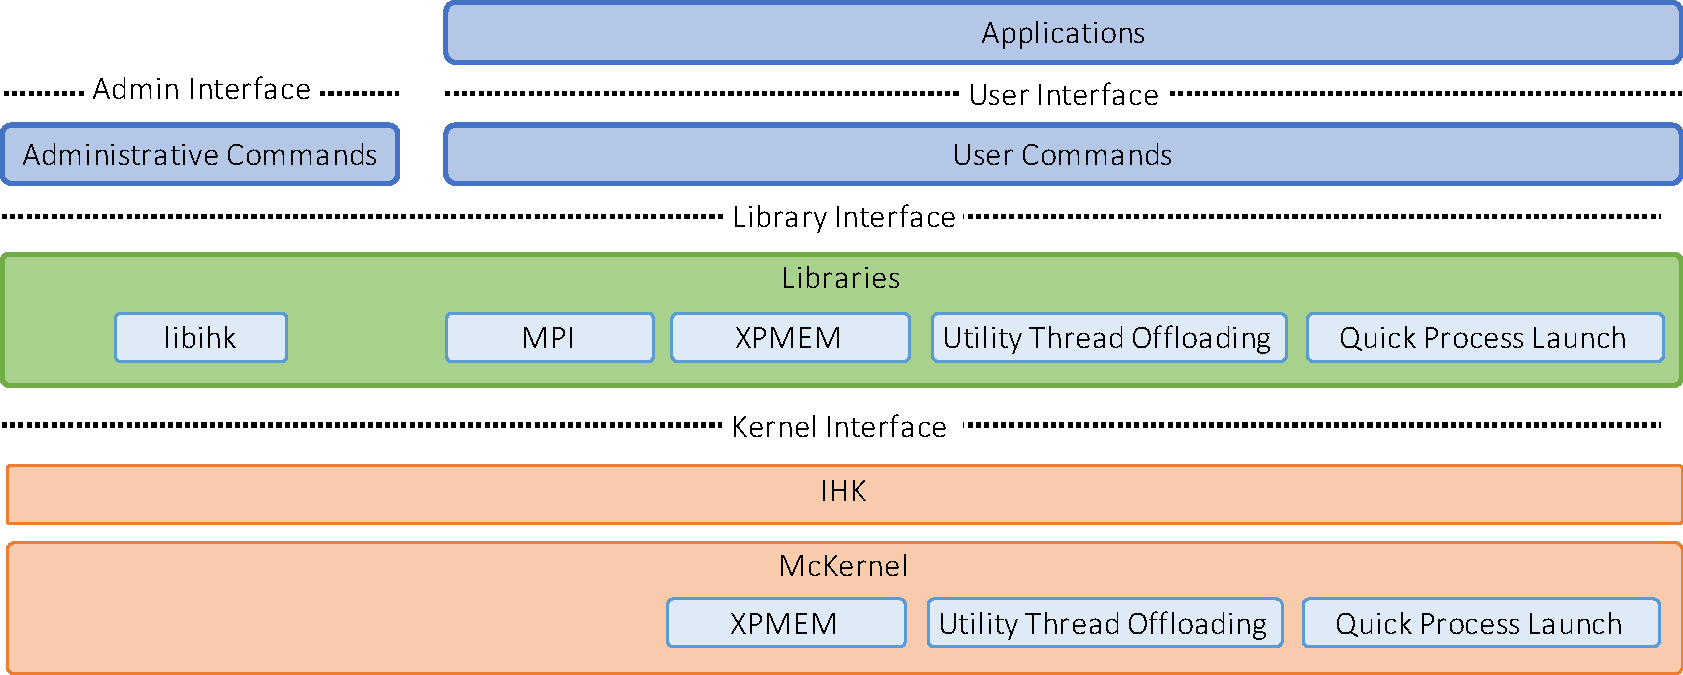
\includegraphics[width=0.9\linewidth]{figs/soft_stack.pdf}
\vspace{-0em}\caption{McKernel software stack}
\label{fig:soft_stack}
\vspace{-0em}
\end{figure}
\FloatBarrier
%
McKernelのソフトウェアスタックを図\ref{fig:soft_stack}に示す。
本章では、ユーザ向けのUser Intefaceと、アプリ向けのLibrary Interfaceと、コマンドやライブラリ向けのKernel Interfaceを説明する。

本章の想定読者は、以下の3種類のユーザまたは開発者である。
\begin{itemize}
\item McKernelのコマンドを用いてアプリを実行するユーザ
\item McKernelのライブラリインターフェイスを使用してアプリを開発する開発者
\item McKernelのカーネルインターフェイスを使用してライブラリを開発する開発者
\end{itemize}

\MODAUG{ユーザインターフェイス、ライブラリインターフェイスの関連ファイルは以下の通り。}
なお、インストールディレクトリを\texttt{<install>}とする。
\begin{table}[!ht]
\footnotesize
\begin{tabular}{|p{0.40\linewidth}|p{0.20\linewidth}|p{0.35\linewidth}|} \hline
\multicolumn{1}{|c}{\textbf{インストール先}}&\multicolumn{1}{|c|}{\textbf{インターフェイス}}&\multicolumn{1}{|c|}{\textbf{説明}}\\ \hline \hline
\texttt{<install>/bin/mcexec}&ユーザ&プロセス起動コマンド\\ \hline
\ADDAUG{\texttt{<install>/bin/eclair}}&ダンプ解析ツール\\ \hline
\ADDAUG{\texttt{<install>/bin/vmcore2mckdump}}&ダンプ形式変換ツール\\ \hline
\texttt{<install>/rootfs/usr/lib64/libuti.so}&ライブラリ&Utility Thread Offloadingライブラリ\\ \hline
\ADDAUG{\texttt{<install>/include/uti.h}}&ライブラリ&\ADDAUG{Utility Thread Offloadingライブラリヘッダファイル}\\ \hline
\ADDAUG{\texttt{<install>/include/qlmpilib.h}}&ライブラリ&\ADDAUG{高速プロセス起動ヘッダファイル}\\ \hline
\ADDAUG{\texttt{<install>/lib/libqlmpi.so}}&ライブラリ&\ADDAUG{高速プロセス起動ライブラリ}\\ \hline
\ADDAUG{\texttt{<install>/lib/libqlfort.so}}&ライブラリ&\ADDAUG{高速プロセス起動ライブラリ(Fortranプログラム用)}\\ \hline
\ADDAUG{\texttt{<install>/lib/libxpmem.so}}    &ライブラリ&\ADDAUG{XPMEMライブラリ}\\ \hline
\ADDAUG{\texttt{<install>/include/xpmem.h}}    &ライブラリ&\ADDAUG{XPMEMライブラリヘッダファイル}\\ \hline
\end{tabular}
\vspace{-0em}
\end{table}
\FloatBarrier

以下、これら3種のインターフェイスを説明する。

\section{\MODMARS{プロセス起動コマンド}}\label{sec:mcexec}
\subsubsection*{書式}{\quad} 
\texttt{
mcexec
 {\lbrack}-c <cpu\_id>{\rbrack}
 {\lbrack}-n <nr\_partitions>{\rbrack}
 {\lbrack}-t <nr\_threads>{\rbrack}\\
\MODMAR{{\lbrack}-M (--mpol-threshold=)<min>{\rbrack}}
 {\lbrack}-h (--extend-heap-by=)<stride>{\rbrack}}\\
\ADDMAR{\texttt{{\lbrack}-s (--stack-premap=){\lbrack}<premap\_size>{\rbrack}{\lbrack},<max>{\rbrack}{\rbrack}}}
\texttt{{\lbrack}--mpol-no-heap{\rbrack}
 {\lbrack}--mpol-no-bss{\rbrack}\\
 {\lbrack}--mpol-no-stack{\rbrack}
 {\lbrack}--mpol-shm-premap{\rbrack}
\ADDMAR{{\lbrack}-m <numa\_node>{\rbrack}}
 {\lbrack}--disable-sched-yield{\rbrack}
\ADDMAR{{\lbrack}-O{\rbrack}}
 {\lbrack}<os\_index>{\rbrack}\\
 <program> {\lbrack}<args>...{\rbrack}
}
\subsubsection*{オプション}{\quad} 
\begin{table}[!ht]
\footnotesize
\begin{tabular}{|p{0.34\linewidth}|p{0.56\linewidth}|} \hline
\texttt{-c <cpu\_id>}&\MODJULTWO{\texttt{mcexec}を実行するCPUの番号を\texttt{<cpu\_id>}に設定する。指定がない場合は0が用いられる。}\\ \hline
\MODMAR{\texttt{-n <nr\_partitions>}}&\ADDMAR{1計算ノードのCPU群を\texttt{<nr\_partitions>}の区画に分割し、第$i$番目に起動された\texttt{mcexec}プロセスから起動されるMcKernelスレッドが第$i$番目の区画のみを利用するように設定する。
分割は物理コア単位で行われる。
%分割方法は2通りあり、\texttt{ikc\_map}(「IHK Specifications」参照)が設定されている際はこのマップに従って分割し、そうでない場合は物理コア単位で分割する。
こうすることで、1ノード\texttt{<nr\_partitions>}プロセスのMPI+OpenMP実行においてCPUを適切に使い分けることができる。}
\\ \hline
\texttt{-t <nr\_threads>}&\MODAUG{\texttt{mcexec}のスレッド数を\texttt{<nr\_threads>}に設定する。このオプションが指定されない場合は、\texttt{OMP\_NUM\_THREADS}環境変数が定義されている場合はその値+4に設定し、存在しない場合はMcKernelに割り当てられたCPU数+4に設定する。\texttt{mcexec}スレッドはMcKernelからの要求を処理する。同時に多くの要求がなされる可能性があるため、この数は〈$\mbox{McKernelのスレッド数}+\alpha$〉に設定する必要がある。}\\ \hline
\texttt{\MODMAR{-M} (--mpol-threshold=)<min>}&\MODAUG{\texttt{<min>}以上のサイズのメモリを要求したときのみ、ユーザが設定したメモリ割り当てポリシが適用されるようにする。\texttt{<min>}はK, M, G(k, m, gでもよい)の単位を付けた場合、それぞれKiB, MiB, GiBの指定になる。指定がない場合はサイズに関係なくユーザが設定したメモリ割り当てポリシが適用される。}\\ \hline
\MODAUG{\texttt{-h (--extend-heap-by=)<step>}}&\MODAUG{ヒープの拡大時にヒーブサイズを少なくとも\texttt{<step>}バイト拡大する。また、ヒープの終了アドレスをラージページサイズにアラインする。\texttt{<step>}はK, M, G(k, m, gでもよい)の単位を付けた場合、それぞれKiB, MiB, GiBの指定になる。指定がない場合は4~KBが用いられる。}\\ \hline
\begin{tabular}[t]{@{}l@{}}\ADDMAR{\texttt{-s (--stack-premap=)}}\\\ADDMAR{\texttt{<premap\_size>,<max>}}\end{tabular}&\ADDMAR{プロセス生成時にスタック領域のうち\texttt{<premap\_size>}バイトをプリマップする。また、スタックの最大サイズを\texttt{<max>}に設定する。\texttt{<premap\_size>, <max>}はK, M, G(k, m, gでもよい)の単位を付けた場合、それぞれKiB, MiB, GiBの指定になる。指定がない場合、\texttt{<premap\_size>}は2~MB、\texttt{<max>}は\texttt{ulimit}コマンドまたは\texttt{setrlimit()}システムコールで設定された値が用いられる。}\\ \hline
\texttt{--mpol-no-heap}&ヒープへのメモリ割り当て時にユーザの設定したメモリ割り当てポリシに従わない。\\ \hline
\texttt{--mpol-no-stack}&スタックへのメモリ割り当て時にユーザの設定したメモリ割り当てポリシに従わない。\\ \hline
\texttt{--mpol-no-bss}&bssへのメモリ割り当て時にユーザの設定したメモリ割り当てポリシに従わない。\\ \hline
\texttt{--mpol-shm-premap}&\MODAUG{\texttt{/dev/shmを}用いた共有メモリをプリマップする。}\\ \hline
%\texttt{--no-bind-ikc-map}&\texttt{-n}オプションを指定した際に、McKernelで使用するCPU集合の分割について、\texttt{ikc\_map}の指定を用いず、NUMAノードで分割する。\\ \hline
\ADDMAR{\texttt{-m <numa\_node>}}&\ADDMAR{メモリを\texttt{<numa\_node>}番目のNUMAノードから割り当てる。割り当てが不可能な場合は他のNUMAノードから割り当てる。}\\ \hline
\texttt{--disable-sched-yield}&\texttt{sched\_yield()}関数を何も行わない関数に置き換える。\\ \hline
\ADDMAR{\texttt{-O}}&\ADDMAR{McKernelに割り当てられたCPU数より大きい数のスレッドまたはプロセスの生成を許可する。指定がない場合は許可しない。許可されていない場合に、CPU数より大きい数のスレッドまたはプロセスを\texttt{clone(), fork(), vfork()}などで生成しようとすると、当該システムコールが\texttt{EINVAL}エラーを返す。}\\ \hline
\texttt{<os\_index>}&プロセス起動先OSインスタンスを\texttt{<os\_index>}番に設定する。省略した場合は0番のOSインスタンスに起動する。\\ \hline
\end{tabular}
\vspace{-0em}
\end{table}
\FloatBarrier

\subsubsection*{説明}{\quad}
\MODAUG{\texttt{<program>}で指定された実行可能ファイルを\texttt{args}で指定された引数で、McKernel上に起動する。}

\texttt{mcexec}の動作を変える環境変数は以下の通り。
\begin{table}[!ht]
\footnotesize
\begin{tabular}{|p{0.25\linewidth}|p{0.70\linewidth}|} \hline
\multicolumn{1}{|c}{\textbf{書式}}&\multicolumn{1}{|c|}{\textbf{説明}}\\ \hline \hline
\begin{tabular}[t]{@{}l@{}}
\texttt{MCEXEC\_WL=<path1>}\\
\texttt{\lbrack:<path2>...\rbrack}\\
\end{tabular}
&\begin{tabular}[t]{@{}l@{}}
\texttt{<path1>, <path2>, ...}以下に存在するMcKernel用実行ファイルについて、\\
\texttt{mcexec}の指定を省略する。なお、指定ディレクトリ以下に実行可能ファイル\\
が存在しても、以下のケースではLinuxで実行される。\\
\textbullet~~\ADDAUG{McKernelが動作していない場合}\\
\textbullet~~\ADDAUG{コマンドが64ビットELFバイナリではない場合}\\
\textbullet~~\ADDAUG{コマンド名が \texttt{mcexec}, \texttt{ihkosctl}, \texttt{ihkconfig}である場合}\\
\end{tabular}\\\hline
\textttw{MCEXEC\_ALT\_ROOT=<path>}&\texttt{ld-linux.so}などのローダを探す際に、\texttt{<path>}と実行可能ファイルの\texttt{.interp}セクションに記載されたパスを結合したパスを探す。\\ \hline
\textttw{MCKERNEL\_RLIMIT\_STACK=<premap\_size>,<max>}&\ADDMAR{(非推奨)プロセス生成時にスタック領域のうち\texttt{<premap\_size>}バイトをプリマップする。また、スタックの最大サイズを\texttt{<max>}に設定する。\texttt{<premap\_size>, <max>}はK, M, G(k, m, gでもよい)の単位を付けた場合、それぞれKiB, MiB, GiBの指定になる。指定がない場合、\texttt{<premap\_size>}は2~MB、\texttt{<max>}は\texttt{ulimit -s}コマンドまたは\texttt{setrlimit()}システムコールで設定された値が用いられる。なお、本環境変数の代わりに\texttt{mcexec}の\texttt{--stack-premap}オプションを使用することを推奨する。}\\\hline
\end{tabular}
\vspace{-0em}
\end{table}
\FloatBarrier

使用例は以下の通り。この例では\texttt{ls -ls}をMcKernel上で実行する。
\begin{verbatim}
$ mcexec ls -ls
\end{verbatim}

\subsubsection*{戻り値}{\quad}
\texttt{<program>}のexit statusを返す。

\section{\MODAUGS{ダンプ採取・解析}}
カーネルダンプの採取と解析のステップは以下の通り。
\begin{enumerate}
\item 以下のいずれかの方法でダンプファイルを作成する。
\begin{enumerate}
\item IHKの関数\texttt{ihk\_os\_makedumpfile()}またはIHKのコマンド\texttt{ihkosctl}を用いて、McKernel形式のダンプファイルを作成する。
\item Linuxのpanicを契機に\texttt{makedumpfile}形式のダンプファイルを作成する。また、コマンド\texttt{vmcore2mckdump}を用いてMcKernel形式に変換する。
\end{enumerate}
\item eclairと呼ぶコマンドを用いてダンプファイルを解析する。
\end{enumerate}
%
以下、関連コマンドのインターフェイスを説明する。

\subsection{\ADDAUGS{ダンプ解析コマンド}}\label{sec:eclair_gaibu}
\subsubsection*{書式}{\quad} \texttt{eclair [-ch] [-d <dump>] [-k <kimg>] }\MODJULTWO{\texttt{[-o <os\_index>] }}\texttt{[-l] }\MODJULTWO{\texttt{[-i]}}
\subsubsection*{オプション}{\quad}
\begin{table}[!ht]
\footnotesize
\begin{tabular}{|p{0.15\linewidth}|p{0.80\linewidth}|} \hline
\texttt{-c}&NMI受付時のコンテキストをスレッドとして扱う。それぞれのコンテキストは\texttt{1000000+〈CPU番号〉}というTIDを持つスレッドとして扱われる。スレッドとして扱うことで、割り込み処理のバックトレースを表示することができる。\\ \hline
\texttt{-h}&利用法を表示する。\\ \hline
\texttt{-d <dump>}&ダンプファイル名を指定する。指定がない場合は\texttt{mcdump}が用いられる。\\ \hline
\texttt{-k <kimg>}&カーネルイメージファイル名を指定する。指定がない場合は\texttt{kernel.img}が用いられる。\\ \hline
\MODJULTWO{\texttt{-o <os\_index>}}&\MODJULTWO{OSインスタンスのインデックスを指定する。指定がない場合は0が用いられる。}\\ \hline
\texttt{-l}&run-queueにユーザスレッドが存在しないCPUについて、\texttt{idle()}を実行しているスレッドが存在するように見せかける。\\ \hline
\ADDJULTWO{\texttt{-i}}&\ADDJULTWO{Interactive modeと呼ぶ、デバッグ対象マシンに存在するメモリを直接参照した解析を行う。なお、ダンプ時にinteractive modeを指定する必要がある。}\\ \hline
\end{tabular}
\vspace{-0em}
\end{table}
\FloatBarrier

\subsubsection*{説明}{\quad}
\MODAUG{\texttt{<dump>}で指定されたeclair形式のダンプファイルを\texttt{<os\_index>}で指定されたOSインデックスを持つOSとして、\texttt{<kimg>}で指定されたカーネルイメージファイルを使って解析する。}

ダンプ解析コマンド内では、gdbが動作しており、gdbと同じコマンドを利用できる。
McKernelは、マルチスレッドの単一プロセスに見える。
まず、最初に、以下のコマンドを実行して、ダンプ解析コマンドにスレッド一覧を覚えさせる必要がある。
\begin{verbatim}
(eclair) info threads
\end{verbatim}
quitコマンド実行時に、inferiorの切り離し許可をユーザに求める。これには、yと応答すること。
ダンプ解析コマンドは,gdbのコマンドの,btコマンドとxコマンドをサポートする.

\subsection{\ADDAUGS{ダンプ形式変換コマンド}}\label{sec:vmcore2mckdump_if}
\subsubsection*{書式}{\quad} \texttt{vmcore2mckdump <vmcore>  <file\_name>}
\subsubsection*{オプション}{\quad}
\begin{table}[!ht]
\footnotesize
\begin{tabular}{|p{0.20\linewidth}|p{0.70\linewidth}|} \hline
\texttt{<vmcore>}&\texttt{makedumpfile}形式のダンプファイルのファイル名\\ \hline
\texttt{<file\_name>}&変換先ダンプファイルのファイル名\\ \hline
\end{tabular}
\vspace{-0em}
\end{table}
\FloatBarrier

\subsubsection*{説明}{\quad}
\texttt{<vmcore>}で指定された\texttt{makedumpfile}形式のダンプファイルからMcKernelに関連する部分を取り出し\texttt{<file\_name>}で指定されたファイルにeclair形式で出力する。
%変換作業はcrashプラグインを用いて行われる。

\section{\MODAUGS{高速プロセス起動ライブラリインターフェイス}}

\comment{
外部仕様の概要を表\ref{tab:spec_ql}に示す。
%
\begin{table}[!htb]
\centering
\footnotesize
\caption{高速プロセス起動コマンド外部仕様概要}\vspace{0.0em}
\label{tab:spec_ql}
\begin{tabular}{|p{0.25\linewidth}|p{0.65\linewidth}|} \hline
\multicolumn{1}{|c}{\textbf{コマンド名}}&\multicolumn{1}{|c|}{\textbf{説明}}\\ \hline \hline
\texttt{ql\_mpiexec\_start}&指定したMPIプロセスが既に存在するか確認し、存在しない場合は\texttt{mpiexec}をバックグラウンドで起動することでMPIプロセスを起動し、存在を記録する。存在する場合は当該MPIプロセスに実行の再開を指示する。本コマンドは当該MPIプロセスが一回の計算を終了すると終了する。\\ \hline
\texttt{ql\_mpiexec\_finalize}&指定したMPIプロセスとその親である\texttt{mpiexec}を終了する。MPIプロセスは終了指示を受けると、\texttt{MPI\_Finalize()}および後続処理を行い終了する。\\ \hline
\ADDAUG{\texttt{ql\_client()}}&\ADDAUG{MPIプログラムが一回の計算が完了した時点で呼び出すライブラリ関数で、再開指示待ちおよび次の計算のための引数と環境変数の設定を行う。}\\ \hline
\end{tabular}
\vspace{-0em}
\end{table}
\FloatBarrier
}

McKernelは、複数種のMPIプログラムを起動しさらにそれを繰り返すジョブにおいてMPIプログラム起動時間を短縮する機能を提供する。
利用例は以下の通り。
\begin{itemize}
\item アンサンブルシミュレーションとデータ同化を繰り返す気象アプリケーション\\
このアプリではジョブスクリプトでそれぞれのMPIプログラムを交互に起動する。この起動時間を短縮する。
\end{itemize}

本機能を利用するためにはジョブスクリプトとアプリケーションを修正する必要がある。ジョブスクリプトの修正方法を例を用いて説明する。
\subsubsection*{修正前}
\small
\begin{verbatim}
/* アンサンブルシミュレーションと同化を10回繰り返す */
for i in {1..10}; do

     /* 100ノードを用いるアンサンブルシミュレーションを10個並列に動作させる */
    for j in {1..10}; do
         mpiexec -n 100 -machinefile ./list1_$j p1.out a1 & pids[$i]=$!;
    done

    /* p1.outの終了を待つ */
    for j in {1..10}; do wait ${pids[$j]}; done

    /* アンサンブルシミュレーションで用いたのと同じ1000ノードを用いてデータ同化
       を行う */
    mpiexec -n 1000 -machinefile ./list2 p2.out a2
done
\end{verbatim}
\normalsize
\subsubsection*{修正後}
\small
\begin{verbatim}
for i in {1..10}; do
    for j in {1..10}; do
        /*  mpiexecをql_mpiexec_startに置き換える */
        ql_mpiexec_start -n 100 -machinefile ./list1_$j p1.out a1 & pids[$j]=$!;
    done

    for j in {1..10}; do wait ${pids[$j]}; done

    ql_mpiexec_start -n 1000 -machinefile ./list2 p2.out a2
done

/* p1.outとp2.outは常駐しているため、ql_mpiexec_finalizeで終了させる。
   mpiexecへの引数と実行可能ファイル名でMPIプログラムを識別しているため、
   実行時と同じものを指定する。 */
for j in {1..10}; do
   ql_mpiexec_finalize -machinefile ./list1_$i p1.out a1;
done
ql_mpiexec_finalize -machinefile ./list2 p2.out a2;
\end{verbatim}
\normalsize

アプリケーションの修正方法を擬似コードを用いて説明する。計算を何度も行えるようなループ構造を持たせ、また\texttt{ql\_client()}を計算完了後に呼び出すようにする。
\small
\begin{verbatim}
    MPI_Init();
    先行・後続MPIプログラムとの通信準備
loop:
    foreach (Fortranの)モジュール
        コマンドライン引数・パラメタファイル・環境変数を用いた初期化処理
    先行MPIプログラムからのデータ受信・スナップショット読み込み
    計算
    後続MPIプログラムへのデータ送信・スナップショット書き出し
    /* ループボディの終わりにql_client()を挿入する */ 
    if(ql_client() == QL_CONTINUE) { goto loop; }
    MPI_Finalize();
\end{verbatim}
\normalsize

以下、コマンドや関数のインターフェイスを説明する。

\subsection{\ADDAUGS{MPIプロセス開始再開コマンド}}
\subsubsection*{書式}{\quad} \texttt{ql\_mpiexec\_start -machinefile <hostfile> {\lbrack}<mpiopts>...{\rbrack} <exe> {\lbrack}<args>...{\rbrack}}
\subsubsection*{オプション}{\quad}
\begin{table}[!ht]
\footnotesize
\begin{tabular}{|p{0.30\linewidth}|p{0.65\linewidth}|} \hline
\multicolumn{1}{|c}{\textbf{オプション}}&\multicolumn{1}{|c|}{\textbf{内容}}\\ \hline \hline
\texttt{-machinefile <hostfile>}&ホストファイル\\ \hline
\texttt{<mpiopts>}&\texttt{mpiexec}のオプション\\ \hline
\texttt{<exe>}&実行可能ファイル\\ \hline
\texttt{<args>}&実行可能ファイルの引数\\ \hline
\end{tabular}
\vspace{-0em}
\end{table}
\FloatBarrier

\subsubsection*{説明}{\quad}
\texttt{<exe>}で指定されたMPIプログラムを開始する。または再開指示待ちの状態にあるMPIプログラムに次の計算開始を指示する。
%具体的には、指定されたMPIプログラムが未起動の場合は、\texttt{mpiexec}をバックグラウンドで起動することで当該MPIプログラムを起動する。当該MPIプログラムがバックグラウンドで起動している場合は、標準入出力、エラー出力を名前付きパイプで接続し、起動中のMPIプロセスに対して再計算指示を行う。
本コマンドはMPIプログラムの一回の計算の完了と共に終了する。
また、MPIプログラムは\texttt{<hostfile>}の内容、\texttt{<mpiopts>}、\texttt{<exe>}とで識別する。

\texttt{ql\_mpiexec\_\{start,finalize\}}コマンドからMPIプログラムに次の動作、引数、環境変数を渡すために用いるファイルは、環境変数\texttt{QL\_PARAM\_PATH}が定義されている場合はその下に、そうでない場合はホームディレクトリ下に作成される。当該ディレクトリは\texttt{ql\_mpiexec\_start}コマンドを実行するノード、各MPIプロセスが実行される計算ノードからアクセスできる必要がある。

%なお、全計算ノードでMcKernelのインストールディレクトリが同じである必要がある。
また、環境変数\texttt{MPIEXEC\_TIMEOUT}によるタイムアウトおよび複数の実行可能ファイルの指定はサポートしない。

\subsubsection*{戻り値}{\quad}
\begin{table}[!h]
\footnotesize
\begin{tabular}{|p{0.15\linewidth}|p{0.75\linewidth}|} \hline
\multicolumn{1}{|c}{\textbf{戻り値}}&\multicolumn{1}{|c|}{\textbf{説明}}\\ \hline \hline
\texttt{0}&正常終了\\ \hline
\texttt{0以外}&異常終了\\ \hline
\end{tabular}
\end{table}
\FloatBarrier

\subsubsection*{エラー時出力}{\quad}
エラーメッセージは\texttt{mpiexec}が出力するエラーメッセージの他に\texttt{ql\_mpiexec\_start}独自に以下のメッセージを出力する。
\begin{table}[!h]
\footnotesize
\begin{tabular}{|p{0.50\linewidth}|p{0.45\linewidth}|} \hline
\multicolumn{1}{|c}{\textbf{メッセージ}}&\multicolumn{1}{|c|}{\textbf{意味}}\\ \hline \hline
unknown option: \texttt{<opt>} &未知のオプション \texttt{<opt>}が指定された\\ \hline
bad option: \texttt{<opt>} &オプション \texttt{<opt>}の指定が誤っている\\ \hline
unsupported option: \texttt{<opt>} &オプション \texttt{<opt>}はサポートしていない\\ \hline
\texttt{':'} is unsupported&\texttt{':'} はサポートしていない\\ \hline
unable to read hostfile(\texttt{<hostfile>}): \texttt{<reason>}&\texttt{<hostfile>}を\texttt{<reason>}の理由により読み込めない\\ \hline
could not open hostfile(\texttt{<hostfile>}): \texttt{<reason>}&\texttt{<hostfile>}\texttt{<reason>}の理由によりオープンできない\\ \hline
\texttt{<hostfile>} not exist&\texttt{<hostfile>}が存在しない\\ \hline
specify \texttt{-machinefile} option&\texttt{-machinefile}オプションが指定されていない\\ \hline
no user program&\texttt{<exe>}が指定されていない\\ \hline
socket directory not exist&ソケット通信用のディレクトリが存在しない\\ \hline
\texttt{ql\_server not execution <reason>}&\texttt{ql\_server}の起動に\texttt{<reason>}の理由により失敗した\\ \hline
\texttt{ql\_mpiexec\_start: socket(<reason>)}&\texttt{ql\_mpiexec\_start}コマンドのsocket操作で\texttt{<reason>}のエラーが発生した\\ \hline
\texttt{ql\_mpiexec\_start: bind(<reason>)}&\texttt{ql\_mpiexec\_start}コマンドのbindで\texttt{<reason>}のエラーが発生した\\ \hline
\texttt{ql\_mpiexec\_start: listen(<reason>)} &\texttt{ql\_mpiexec\_start}コマンドのlistenで\texttt{<reason>}のエラーが発生した\\ \hline
\texttt{ql\_mpiexec\_start: connect(<reason>)} &\texttt{ql\_mpiexec\_start}コマンドのconnectで\texttt{<reason>}のエラーが発生した\\ \hline
\end{tabular}
\vspace{-0em}
\end{table}
\FloatBarrier

\subsection{\ADDAUGS{MPIプロセス終了指示コマンド}}
\subsubsection*{書式}{\quad} \texttt{ql\_mpiexec\_finalize -machinefile <hostfile> {\lbrack}<mpiopts>...{\rbrack}  <exe> }
\subsubsection*{オプション}{\quad}
\begin{table}[!ht]
\footnotesize
\begin{tabular}{|p{0.30\linewidth}|p{0.65\linewidth}|} \hline
\multicolumn{1}{|c}{\textbf{オプション}}&\multicolumn{1}{|c|}{\textbf{説明}}\\ \hline \hline
\texttt{-machinefile <hostfile>}&ホストファイル\\ \hline
\texttt{<mpiopts>}&\texttt{mpiexec}のオプション\\ \hline
\texttt{<exe>}&実行可能ファイル\\ \hline
\end{tabular}
\vspace{-0em}
\end{table}
\FloatBarrier
\subsubsection*{説明}{\quad}
\texttt{ql\_mpiexec\_start}によって起動されたMPIプログラムを終了させる。
%処理としては、起動中の当該MPIプロセスに対して、終了指示を出し、バックグラウンドで起動している、\texttt{mpiexec}を終了させる。
本コマンドはMPIプログラムの終了と共に終了する。
また、MPIプログラムは\texttt{<hostfile>}の内容、\texttt{<mpiopts>}、\texttt{<exe>}とで識別する。

%なお、全計算ノードでMcKernelのインストールディレクトリが同じである必要がある。

\subsubsection*{戻り値}{\quad}
\begin{table}[!h]
\footnotesize
\begin{tabular}{|p{0.15\linewidth}|p{0.75\linewidth}|} \hline
\multicolumn{1}{|c}{\textbf{戻り値}}&\multicolumn{1}{|c|}{\textbf{説明}}\\ \hline \hline
\texttt{0}&正常終了\\ \hline
\texttt{0以外}&異常終了\\ \hline
\end{tabular}
\vspace{-0em}
\end{table}
\FloatBarrier

\subsubsection*{エラー時出力}{\quad}
エラーメッセージは\texttt{mpiexec}が出力するエラーメッセージの他に\texttt{ql\_mpiexec\_finalize}独自に以下のメッセージを出力する。
\begin{table}[!h]
\footnotesize
\begin{tabular}{|p{0.50\linewidth}|p{0.45\linewidth}|} \hline
\multicolumn{1}{|c}{\textbf{メッセージ}}&\multicolumn{1}{|c|}{\textbf{意味}}\\ \hline \hline
unknown option: \texttt{<opt>} &未知のオプション\texttt{<opt>}が指定された\\ \hline
bad option: \texttt{<opt>} &オプション\texttt{<opt>}の指定が誤っている\\ \hline
unsupported option: \texttt{<opt>} &オプション\texttt{<opt>}はサポートしていない\\ \hline
\texttt{':'} is unsupported&\texttt{':'} はサポートしていない\\ \hline
unable to read hostfile(\texttt{<hostfile>}): \texttt{<reason>}&\texttt{<hostfile>}を\texttt{<reason>}の理由で読み込めない\\ \hline
could not open hostfile(\texttt{<hostfile>}): \texttt{<reason>}&\texttt{<hostfile>}を\texttt{<reason>}の理由でオープンできない\\ \hline
\texttt{<hostfile>} not exist&ホストファイルが存在しない\\ \hline
specify \texttt{-machinefile} option&\texttt{-machinefile}オプションが指定されていない\\ \hline
no user program&\texttt{<exe>}が指定されていない\\ \hline
socket directory not exist&ソケット通信用のディレクトリが存在しない\\ \hline
not found mpi process&\texttt{mpiexec}プロセスが存在しない\\ \hline
\end{tabular}
\vspace{-0em}
\end{table}
\FloatBarrier

\comment{
\subsection{MPI実行環境初期化関数(C言語関数)}
\subsubsection*{書式}{\quad} \texttt{int MPI\_Init(int *argc,char ***argv)}
\subsubsection*{引数}{\quad}
\begin{table}[!ht]
\footnotesize
\begin{tabular}{|p{0.15\linewidth}|p{0.75\linewidth}|} \hline
\multicolumn{1}{|c}{\textbf{引数}}&\multicolumn{1}{|c|}{\textbf{説明}}\\ \hline \hline
\texttt{argc}&引数の数へのポインタ\\ \hline
\texttt{argv}&引数文字列の配列へのポインタ\\ \hline
\end{tabular}
\vspace{-0em}
\end{table}
\subsubsection*{説明}{\quad}
高速プロセス起動のための初期化を行う。本関数は、PMPIインタフェースにより\texttt{MPI\_Init}を置き換えることで実装される。
%通常のMPI環境初期化と、高速プロセス起動の初期化関数を呼び出す。
%直接mpiexecから呼び出された場合は、通常のMPI環境初期化のみ行う。
\subsubsection*{戻り値}{\quad}
\begin{table}[!ht]
\footnotesize
\begin{tabular}{|p{0.15\linewidth}|p{0.75\linewidth}|} \hline
\multicolumn{1}{|c}{\textbf{戻り値}}&\multicolumn{1}{|c|}{\textbf{説明}}\\ \hline \hline
\texttt{MPI\_SUCCESS}&正常終了\\ \hline
\texttt{MPI\_ERR\_OTHER }&\texttt{MPI\_init()}が複数回実行された\\ \hline
\end{tabular}
\vspace{-0em}
\end{table}
\FloatBarrier

\subsection{MPI実行環境初期化関数(Fortran)}
\subsubsection*{書式}{\quad} \texttt{subroutine MPI\_INIT( ierr )}
\subsubsection*{引数}{\quad}
\begin{table}[!ht]
\footnotesize
\begin{tabular}{|p{0.15\linewidth}|p{0.75\linewidth}|} \hline
\multicolumn{1}{|c}{\textbf{引数}}&\multicolumn{1}{|c|}{\textbf{説明}}\\ \hline \hline
\texttt{ierr}&戻り値\\ \hline
\end{tabular}
\vspace{-0em}
\end{table}
\subsubsection*{説明}{\quad}
fortran用のMPI実行環境初期化関数。処理内容は、C言語用のMPI実行環境初期化関数と同じ。
\subsubsection*{戻り値}{\quad}
\begin{table}[!ht]
\footnotesize
\begin{tabular}{|p{0.15\linewidth}|p{0.75\linewidth}|} \hline
\multicolumn{1}{|c}{\textbf{戻り値}}&\multicolumn{1}{|c|}{\textbf{説明}}\\ \hline \hline
\texttt{MPI\_SUCCESS}&正常終了\\ \hline
\texttt{MPI\_ERR\_OTHER }&\texttt{MPI\_init()}が複数回実行された\\ \hline
\end{tabular}
\vspace{-0em}
\end{table}
\subsubsection*{前提条件}{\quad}
\begin{itemize}
\item[1]fortranは、GNU fortranもしくはIntel fortranを前提とする。
\item[2]Intel fortranを使用する場合は、コンパイルオプションに-shared-intelが必要。
\end{itemize}
\FloatBarrier
}

\subsection{\ADDAUGS{計算の再開・終了関数(C言語)}}
\subsubsection*{書式}{\quad} \texttt{ql\_client(int *argc,char ***argv)}
\subsubsection*{引数}{\quad}
\begin{table}[!ht]
\footnotesize
\begin{tabular}{|p{0.15\linewidth}|p{0.75\linewidth}|} \hline
\multicolumn{1}{|c}{\textbf{引数}}&\multicolumn{1}{|c|}{\textbf{説明}}\\ \hline \hline
\texttt{argc}&引数の数へのポインタ\\ \hline
\texttt{argv}&引数文字列の配列へのポインタ\\ \hline
\end{tabular}
\vspace{-0em}
\end{table}
\subsubsection*{説明}{\quad}
\texttt{ql\_mpiexec\_\{start,finalize\}}コマンドによる指示を待ち、指示結果を返す。
本関数は、MPIプログラム内で、一回の計算の完了後に呼び出す。
%高速プロセス起動の場合は、各プロセスで計算完了の同期をとった後、swapoutのシステムコールを呼び、停止状態となる。停止状態が解除後、再開指示の場合、引数・環境変数を取得し、引数argc,argv及び環境変数を設定し、\texttt{QL\_CONTINUE}を戻り値としてリターンする。終了指示の場合、\texttt{QL\_EXIT}を戻り値としてリターンする。
\comment{スワップファイルは、環境変数\texttt{QL\_SWAP\_PATH}が定義されている場合はそのディレクトリ下に、定義されていない場合は\texttt{/tmp}下に作成される。当該ディレクトリはユーザプログラムが実行されるすべての計算ノードで存在する必要がある。}

\subsubsection*{戻り値}{\quad}
\begin{table}[!ht]
\footnotesize
\begin{tabular}{|p{0.15\linewidth}|p{0.75\linewidth}|} \hline
\multicolumn{1}{|c}{\textbf{戻り値}}&\multicolumn{1}{|c|}{\textbf{説明}}\\ \hline \hline
\texttt{\texttt{QL\_CONTINUE}}&次の計算の開始が指示された\\ \hline
\texttt{\texttt{QL\_EXIT}}&MPIプログラムの終了が指示された、あるいは当該プロセスが\texttt{ql\_mpiexec\_start}コマンドで起動されていない\\ \hline
\end{tabular}
\vspace{-0em}
\end{table}

\subsection{\ADDAUGS{計算の再開・終了関数(Fortran)}}
\subsubsection*{書式}{\quad} \texttt{subroutine QL\_CLIENT(ierr)}
\subsubsection*{引数}{\quad}
\begin{table}[!ht]
\footnotesize
\begin{tabular}{|p{0.10\linewidth}|p{0.10\linewidth}|p{0.75\linewidth}|} \hline
\multicolumn{1}{|c}{\textbf{引数}}&\multicolumn{1}{|c}{\textbf{型}}&\multicolumn{1}{|c|}{\textbf{説明}}\\ \hline \hline
\texttt{ierr}&\texttt{INT}&戻り値\\ \hline
\end{tabular}
\vspace{-0em}
\end{table}
\subsubsection*{説明}{\quad}
MPIプログラム内で一回の計算の完了後に呼び出され、\texttt{ql\_mpiexec\_\{start,finalize\}}コマンドによる指示を待ち、指示結果を返す。
なお、本関数を使用するためにはlibqlfort.soを\texttt{LD\_PRELOAD}でロードする必要がある。
また、コンパイラはGNU Fortran CompilerまたはIntel Fortran Compilerをサポートする。
Intel Fortran Compiler使用時は、コンパイルオプションに-shared-intelを指定する必要がある。

\subsubsection*{戻り値}{\quad}
\begin{table}[!ht]
\footnotesize
\begin{tabular}{|p{0.15\linewidth}|p{0.75\linewidth}|} \hline
\multicolumn{1}{|c}{\textbf{戻り値}}&\multicolumn{1}{|c|}{\textbf{説明}}\\ \hline \hline
\texttt{\texttt{1}}&次の計算の開始が指示された\\ \hline
\texttt{\texttt{0}}&MPIプログラムの終了が指示された、あるいは当該プロセスが\texttt{ql\_mpiexec\_start}コマンドで起動されていない\\ \hline
\end{tabular}
\vspace{-0em}
\end{table}
\FloatBarrier

\section{\ADDMARS{高速プロセス起動カーネルインターフェイス}}
\subsection{\ADDMARS{\texttt{swapout}システムコール}}
\subsubsection*{書式}{\quad} \texttt{int swapout(char *filename, void *workarea, size\_t size, int flag)}
\subsubsection*{引数}{\quad}
\begin{table}[!ht]
\footnotesize
\begin{tabular}{|p{0.15\linewidth}|p{0.75\linewidth}|} \hline
\multicolumn{1}{|c}{\textbf{引数}}&\multicolumn{1}{|c|}{\textbf{説明}}\\ \hline \hline
\texttt{filename}&スワップファイル名へのポインタ\\ \hline
\texttt{workarea}&作業領域へのポインタ\\ \hline
\texttt{size}&作業領域のサイズ\\ \hline
\texttt{flag}&swapoutの動作制御用フラグ \\ \hline
\end{tabular}
\vspace{-0em}
\end{table}
\subsubsection*{説明}{\quad}
プロセスのメモリ領域のファイルへの待避(スワップアウトと呼ぶ)とファイルからの復元(スワップインと呼ぶ)を行う。

処理ステップは以下の通り。
\begin{itemize}
\item[1] \texttt{filename}がNULLまたは\texttt{flag}が1の場合はステップ6に進む。そうでない場合はステップ2に進む。
\item[2] スワップアウト処理を行う。
\item[3] \texttt{flag}が2の場合は、ステップ5に進む。そうでない場合は、ステップ4に進む。
\item[4] \texttt{mcexec}へ制御を移し、スワップアウト完了の同期と、\texttt{ql\_mpiexec\_\{start,finalize\}}による指示を待った後、本システムコールに制御を戻す。
\item[5]  スワップイン処理を行う。さらに呼び出し元に戻る。
\item[6] \texttt{mcexec}へ制御を移し、\texttt{ql\_mpiexec\_\{start,finalize\}}による指示を待った後、本システムコールに制御を戻す。さらに呼び出し元に戻る。
\end{itemize}
\FloatBarrier

\subsubsection*{戻り値}{\quad}
\begin{table}[!h]
\footnotesize
\begin{tabular}{|p{0.15\linewidth}|p{0.75\linewidth}|} \hline
\multicolumn{1}{|c}{\textbf{戻り値}}&\multicolumn{1}{|c|}{\textbf{説明}}\\ \hline \hline
\texttt{0}&正常終了\\ \hline
\texttt{-1}&エラー\\ \hline
\texttt{-ENOMEM}&メモリが不足\\ \hline
\texttt{-EINVAL}&引数が不正\\ \hline
\end{tabular}
\vspace{-0em}
\end{table}

\comment{
\subsection{パフォーマンスカウンタ操作システムコール}
\subsubsection{パフォーマンスカウンタ初期化}
\subsubsection*{書式}{\quad} \texttt{int pmc\_init(int counter, int type)}
\subsubsection*{説明}{\quad}
プロセッサの\texttt{counter}番目のパフォーマンスカウンタを、ユーザモードで発生した、\texttt{type}で指定したイベントをカウントするように設定する。
\texttt{type}にはプロセッサアーキテクチャ依存のイベント種を数値で指定する。

\texttt{x86\_64}アーキテクチャで利用できるイベント種は以下の通り。
\begin{table}[!h]
\footnotesize
\begin{tabular}{|p{0.25\linewidth}|p{0.66\linewidth}|} \hline
\multicolumn{1}{|c}{\textbf{イベント種}}&\multicolumn{1}{|c|}{\textbf{説明}}\\ \hline \hline
\texttt{APT\_TYPE\_INSTRUCTIONS}&発行された命令数\\ \hline
\texttt{APT\_TYPE\_L1D\_REQUEST}&L1データキャッシュへのリクエスト数\\ \hline
\texttt{APT\_TYPE\_L1I\_REQUEST}&L1命令キャッシュへのリクエスト数\\ \hline
\texttt{APT\_TYPE\_L1D\_MISS}&L1データキャッシュミス数\\ \hline
\texttt{APT\_TYPE\_L1I\_MISS}&L1命令キャッシュミス数\\ \hline
\texttt{APT\_TYPE\_L2\_MISS}&L2キャッシュミス数\\ \hline
\texttt{APT\_TYPE\_LLC\_MISS}&Last Level Cache (LLC)ミス数\\ \hline
\texttt{APT\_TYPE\_DTLB\_MISS}&データTLBミス数\\ \hline
\texttt{APT\_TYPE\_ITLB\_MISS}&命令TLBミス数\\ \hline
\texttt{APT\_TYPE\_STALL}&ストールサイクル数\\ \hline
\texttt{APT\_TYPE\_CYCLE}&サイクル数\\ \hline
\end{tabular}
\vspace{-0em}
\end{table}
\FloatBarrier

\subsubsection*{戻り値}
\begin{table}[!h]
\footnotesize
\begin{tabular}{|p{0.20\linewidth}|p{0.66\linewidth}|} \hline
0&正常終了\\ \hline
-EINVAL&\texttt{counter}が負または物理カウンタ数以上\\ \hline
\end{tabular}
\vspace{-0em}
\end{table}
\FloatBarrier

\subsubsection{パフォーマンスカウンタ開始}
\subsubsection*{書式}{\quad} \texttt{int pmc\_start(int counter)}
\subsubsection*{説明}{\quad}
プロセッサの\texttt{counter}番目のパフォーマンスカウンタを開始する。

\subsubsection*{戻り値}
\begin{table}[!h]
\footnotesize
\begin{tabular}{|p{0.20\linewidth}|p{0.66\linewidth}|} \hline
0&正常終了\\ \hline
-EINVAL&\texttt{counter}が負または物理カウンタ数以上\\ \hline
\end{tabular}
\vspace{-0em}
\end{table}
\FloatBarrier

\subsubsection{パフォーマンスカウンタ停止}
\subsubsection*{書式}{\quad} \texttt{int pmc\_stop(int counter)}
\subsubsection*{説明}{\quad}
プロセッサの\texttt{counter}番目のパフォーマンスカウンタを停止する。

\subsubsection*{戻り値}
\begin{table}[!h]
\footnotesize
\begin{tabular}{|p{0.20\linewidth}|p{0.66\linewidth}|} \hline
0&正常終了\\ \hline
-EINVAL&\texttt{counter}が負または物理カウンタ数以上\\ \hline
\end{tabular}
\vspace{-0em}
\end{table}
\FloatBarrier

\subsubsection{パフォーマンスカウンタリセット}
\subsubsection*{書式}{\quad} \texttt{int pmc\_reset(int counter)}
\subsubsection*{説明}{\quad}
プロセッサの\texttt{counter}番目のパフォーマンスカウンタの値を0に設定する。

\subsubsection*{戻り値}
\begin{table}[!h]
\footnotesize
\begin{tabular}{|p{0.20\linewidth}|p{0.66\linewidth}|} \hline
0&正常終了\\ \hline
-EINVAL&\texttt{counter}が負または物理カウンタ数以上\\ \hline
\end{tabular}
\vspace{-0em}
\end{table}
\FloatBarrier
}
\section{\MODAUGS{Utility Thread Offloadingライブラリインターフェイス}}\label{sec:uti_libif}
\comment{
McKernelは、スレッドをLinuxのCPUにマイグレートする機能(Utility Thread Offloadingと呼ぶ)を提供する。
利用方法の例は以下の通り。
\begin{enumerate}
\item MPIランタイムが、通信のプログレスを非同期に行うスレッドをLinuxのCPUに生成する。
%\item MPIランタイムが、実行時にチャネルの切断・再接続を行うスレッドをLinuxのCPUに生成する。
\end{enumerate}
}
インターフェイスは「McKernel仕様付録(Utility thread offloadingライブラリ編)」に記載する。

\comment{
外部仕様の概要を表\ref{tab:spec_libuti}に示す。
%
\begin{table}[!htb]
\centering
\footnotesize
\caption{Utility Thread Offloadingライブラリ外部仕様概要}\vspace{0.0em}
\label{tab:spec_libuti}
\begin{tabular}{|p{0.40\linewidth}|p{0.55\linewidth}|} \hline
\multicolumn{1}{|c}{\textbf{関数・環境変数・マクロ名}}&\multicolumn{1}{|c|}{\textbf{説明}}\\ \hline \hline
\texttt{uti\_attr\_init()}&資源ポリシーと振る舞いを記述する属性オブジェクトを初期化する\\ \hline
\texttt{uti\_attr\_destroy()}&\MODAUG{属性オブジェクトを破棄する}\\ \hline
\texttt{UTI\_CPU\_SET}(環境変数)&指定のCPUセットへの配置を指示\\ \hline
\texttt{UTI\_ATTR\_NUMA\_SET}(マクロ)&指定のNUMAノードセット利用を指示\\ \hline
\texttt{UTI\_ATTR\_SAME\_NUMA\_DOMAIN}(マクロ)&呼び出し元と同一のNUMAノード利用を指示\\ \hline
\texttt{UTI\_ATTR\_DIFFERENT\_NUMA\_DOMAIN}(マクロ)&呼び出し元と異なるNUMAノード利用を指示\\ \hline
\texttt{UTI\_ATTR\_SAME\_\{L1,L2,L3\}}(マクロ)&呼び出し元とL1、L2、L3を共有するCPUへの配置を指示\\ \hline
\texttt{UTI\_ATTR\_DIFFERENT\_\{L1,L2,L3\}}(マクロ)&呼び出し元とL1、L2、L3を共有しないCPUへの配置を指示\\ \hline
\texttt{UTI\_ATTR\_EXCLUSIVE\_CPU}(マクロ)&コアを専有させないと正常動作しないことを示唆\\ \hline
\texttt{UTI\_ATTR\_CPU\_INTENSIVE}(マクロ)&CPUインテンシブを示唆\\ \hline
\texttt{UTI\_ATTR\_HIGH\_PRIORITY}(マクロ)&スケジュールでの高い優先度付与が有益であることを示唆\\ \hline
\texttt{UTI\_ATTR\_NON\_COOPERATIVE}(マクロ)&cooperative scheduling不使用を示唆\\ \hline
\texttt{uti\_pthread\_create()}&pthread互換スレッドを属性オブジェクトの内容に基づいてシステムサービス用CPUに作成する\\ \hline
\end{tabular}
\vspace{-0em}
\end{table}
\FloatBarrier
}

\section{\MODAUGS{Utility Thread Offloadingカーネルインターフェイス}}
McKernelは、スレッドをLinuxのCPUにマイグレートする機能(Utility Thread Offloading, UTIと呼ぶ)を提供する。
UTIのカーネルインターフェイスは、第\ref{sec:uti_libif}節で説明するライブラリによって用いられる。

以下、関連システムコールのインターフェイスを説明する。

\subsection{McKernelスレッドのLinuxへのマイグレートシステムコール}
\subsubsection*{書式}{\quad} \texttt{int util\_migrate\_inter\_kernel(uti\_attr\_t *attr)}
\subsubsection*{説明}{\quad}
\texttt{attr}と環境変数\texttt{UTI\_CPU\_SET}で指定された、CPU位置とスレッドの振る舞いの記述に基づき、呼び出し元スレッドをLinux CPUにマイグレートさせる。

環境変数\texttt{UTI\_CPU\_SET}はビットマップ形式でCPU位置を示す。また、\texttt{uti\_attr\_t}は以下のように定義される。
\small
\begin{verbatim}
#define UTI_MAX_NUMA_DOMAINS (1024)

typedef struct uti_attr {
    uint64_t numa_set[(UTI_MAX_NUMA_DOMAINS + 63) / 64];
    /* スレッド配置先NUMAノードを表すビットマップ */
    uint64_t flags;
    /* CPU位置とスレッドの振る舞いを表すビットマップ */
} uti_attr_t;
\end{verbatim}
\normalsize

\texttt{uti\_attr\_t}の\texttt{flags}はビットマップで、ビット1は対応するCPU位置の指示または振る舞いの記述が有効であることを示す。ビット位置と指示・記述の対応は以下の通り。
\small
\begin{verbatim}
#define UTI_FLAG_NUMA_SET (1ULL<<1)
/* numa_setフィールドで指定したNUMAノードへ配置する */
#define UTI_FLAG_SAME_NUMA_DOMAIN (1ULL<<2)
/* 呼び出し元と同一NUMAノードへ配置する */
#define UTI_FLAG_DIFFERENT_NUMA_DOMAIN (1ULL<<3)
/* 呼び出し元とは異なるNUMAノードへ配置する */
#define UTI_FLAG_SAME_L1 (1ULL<<4)
#define UTI_FLAG_SAME_L2 (1ULL<<5)
#define UTI_FLAG_SAME_L3 (1ULL<<6)
/* 呼び出し元とそれぞれのレベルのキャッシュを共有するCPUへ配置する */
#define UTI_FLAG_DIFFERENT_L1 (1ULL<<7)
#define UTI_FLAG_DIFFERENT_L2 (1ULL<<8)
#define UTI_FLAG_DIFFERENT_L3 (1ULL<<9)
/* 呼び出し元とそれぞれのレベルのキャッシュを共有しないCPUへ配置する */
#define UTI_FLAG_EXCLUSIVE_CPU (1ULL<<10)
/* CPUを専有させると効率的に動作する。
   例えば、mwait命令を用いている。*/
#define UTI_FLAG_CPU_INTENSIVE (1ULL<<11)
/* CPUサイクルを多く使用する。例えば、ネットワーク
   デバイスのイベントキューを繰り返しポーリングする。*/
#define UTI_FLAG_HIGH_PRIORITY (1ULL<<12)
/* スケジューラのプライオリティを上げると効率的に動作する。
   例えば、ネットワークデバイスのイベント待ちをする。*/
#define UTI_FLAG_NON_COOPERATIVE (1ULL<<13)
/* co-operativeスケジューリングを行っていない。例えば、
   イベント待ちになった際にsched_yield()を呼ぶ、ということをしない。*/
\end{verbatim}
\normalsize

なお、McKernelからLinuxへの1度のマイグレートのみ可能である。
 
\subsubsection*{戻り値}{\quad}
\begin{table}[!ht]
\footnotesize
\begin{tabular}{|p{0.20\linewidth}|p{0.66\linewidth}|} \hline
0&正常終了\\ \hline
-1&エラー\\ \hline
\end{tabular}
\vspace{-0em}
\end{table}
\FloatBarrier

\subsubsection*{エラー時の\texttt{errno}の値}{\quad}
\begin{table}[!ht]
\footnotesize
\begin{tabular}{|p{0.20\linewidth}|p{0.66\linewidth}|} \hline
\texttt{-ENOSYS}&\texttt{util\_migrate\_inter\_kernel}がサポートされていない。\\ \hline
\texttt{-EFAULT}&\texttt{attr}にアクセスできない。\\ \hline
\end{tabular}
\vspace{-0em}
\end{table}
\FloatBarrier


\subsection{スレッド生成先OS指定システムコール}
\subsubsection*{書式}{\quad} \texttt{int util\_indicate\_clone(int mod, uti\_attr\_t *attr)}
\subsubsection*{説明}{\quad}
呼び出し元スレッドが発行する\texttt{clone}システムコールの動作を変え、スレッド生成後直ちに\texttt{mod}に指定したOSへマイグレートさせる。CPU位置とLinuxのスケジューラ設定は、\texttt{attr}と環境変数\texttt{UTI\_CPU\_SET}で指定されたヒントに基づいて決定される。
この関数は、\texttt{pthread\_create()}などでLinuxへスレッドを生成させるために用いる。
本関数も、\texttt{util\_migrate\_inter\_kernel}と同様、McKernelからLinuxへの1度のマイグレートのみ可能である。

\texttt{mod}の取りうる値と意味は以下の通り。
\begin{table}[!ht]
\footnotesize
\begin{tabular}{|p{0.20\linewidth}|p{0.66\linewidth}|} \hline
\texttt{SPAWN\_TO\_REMOTE}&Linuxへ生成\\ \hline
\texttt{SPAWN\_TO\_LOCAL}&McKernelへ生成\\ \hline
\end{tabular}
\vspace{-0em}
\end{table}
\FloatBarrier

\subsubsection*{戻り値}{\quad}
\begin{table}[!ht]
\footnotesize
\begin{tabular}{|p{0.20\linewidth}|p{0.66\linewidth}|} \hline
0&正常終了\\ \hline
-1&エラー\\ \hline
\end{tabular}
\vspace{-0em}
\end{table}
\FloatBarrier

\subsubsection*{エラー時の\texttt{errno}の値}{\quad}
\begin{table}[!ht]
\footnotesize
\begin{tabular}{|p{0.20\linewidth}|p{0.66\linewidth}|} \hline
\texttt{ENOSYS}& \texttt{util\_indicate\_clone}がサポートされていない。\\ \hline
\texttt{EINVAL}& \texttt{mod}に未定義の値を指定した。\\ \hline
\texttt{EFAULT}& \texttt{attr}にアクセスできない。\\ \hline
\end{tabular}
\vspace{-0em}
\end{table}
\FloatBarrier

\subsection{カーネル種別取得システムコール}
\subsubsection*{書式}{\quad} \texttt{int get\_system()}
\subsubsection*{説明}{\quad}
呼び出し元スレッドが動作しているOSの種別を返却する。
なお、本関数の名称は次バージョンにて\texttt{is\_mckernel()}等に変更される予定である。

\subsubsection*{戻り値}
\begin{table}[!ht]
\footnotesize
\begin{tabular}{|p{0.20\linewidth}|p{0.66\linewidth}|} \hline
0&OSがMcKernel\\ \hline
-1&エラー(OSがLinux)\\ \hline
\end{tabular}
\vspace{-0em}
\end{table}
\FloatBarrier

\subsubsection*{エラー時の\texttt{errno}の値}{\quad}
\begin{table}[!ht]
\footnotesize
\begin{tabular}{|p{0.20\linewidth}|p{0.66\linewidth}|} \hline
\texttt{ENOSYS}&Linuxで呼び出した\\ \hline
\end{tabular}
\vspace{-0em}
\end{table}
\FloatBarrier


\section{\ADDAUGS{XPMEMライブラリインターフェイス}}\label{sec:xpmem_libif}
XPMEMを使うことによって、あるプロセスがマップしたメモリ領域を他のプロセスからマップできるようになる。
利用方法は以下の通り。第1のプロセスのメモリ領域を第2のプロセスがマップしようとしているとする。
\begin{enumerate}
\item 第1のプロセスがメモリ領域を\texttt{xpmem\_make()}を用いてXPMEM segmentとして登録する。また、segment idを第2のプロセスに渡す。
\item 第2のプロセスが\texttt{xpmem\_get()}で当該XPMEM segmentに対するアクセス許可を得る。
\item 第2のプロセスが\texttt{xpmem\_attach()}で当該XPMEM segmentを自身の仮想アドレス範囲にマップする。
\item 第2のプロセスが当該メモリ領域に対する操作を行う。
\item 第2のプロセスが\texttt{xpmem\_detach()}で当該メモリ領域をアンマップする。
\item 第2のプロセスが\texttt{xpmem\_release()}で当該XPMEM segmentに対するアクセス許可が不要になったことをドライバに伝える。
\item 第1のプロセスが\texttt{xpmem\_remove()}を用いて当該XPMEM segmentを破棄する。
\end{enumerate}

以下、関連関数のインターフェイスを説明する。

\comment{
\subsection{Copyright}
\begin{verbatim}
/*
 * This file is subject to the terms and conditions of the GNU Lesser General
 * Public License.  See the file ``COPYING.LESSER'' in the main directory of
 * this archive for more details. The underlying library is subject to the
 * terms and conditions of the GNU Lesser General Public License.
 *
 * Copyright (c) 2004-2007 Silicon Graphics, Inc.  All Rights Reserved.
 * Copyright (c) 2016      Nathan Hjelm. All rights reserved.
 */
\end{verbatim}
}

\subsection{Get Version Number}
\subsubsection*{書式}{\quad}
\texttt{int xpmem\_version (void)}
\subsubsection*{説明}{\quad}
This function gets the XPMEM version.
\subsubsection*{戻り値}{\quad}
\begin{table}[!h]
\footnotesize
\begin{tabular}{|p{0.20\linewidth}|p{0.66\linewidth}|} \hline
$\ne -1$&XPMEM version number\\ \hline
-1&Failure\\ \hline
\end{tabular}
\vspace{-0em}
\end{table}
\FloatBarrier

\subsection{Expose Memory Block}
\subsubsection*{書式}{\quad}
\begin{verbatim}
xpmem_segid_t xpmem_make(
        void *vaddr,
        size_t size,
        int permit_type,
        void *permit_value)
\end{verbatim}
\subsubsection*{説明}{\quad}
\texttt{xpmem\_make()} shares a memory block specified by \texttt{vaddr} and \texttt{size} by invoking the XPMEM driver.
\texttt{permit\_type} is for the future extension. Use \texttt{XPMEM\_PERMIT\_MODE} for this version.
\texttt{permit\_value} specifies the permissions mode expressed as an octal value.

This function is expected to be called by the source process to obtain a segment ID to share with other
processes. It is common to call this function with \texttt{vaddr} = NULL and
\texttt{size} = \texttt{XPMEM\_MAXADDR\_SIZE}. This will share the entire address space of
the calling process.

\subsubsection*{戻り値}{\quad}
\begin{table}[!h]
\footnotesize
\begin{tabular}{|p{0.20\linewidth}|p{0.66\linewidth}|} \hline
$\ne -1$&64-bit segment ID (\texttt{xpmem\_segid\_t})\\ \hline
-1&Failure\\ \hline
\end{tabular}
\vspace{-0em}
\end{table}
\FloatBarrier

\subsection{Un-Expose Memory Block}
\subsubsection*{書式}{\quad}
\begin{verbatim}
static int xpmem_remove(xpmem_segid_t segid)
\end{verbatim}

\subsubsection*{説明}{\quad}
The opposite of \texttt{xpmem\_make()}, this function deletes the mapping specified by 
\texttt{segid} that was created from a previous \texttt{xpmem\_make()} call. 
All the attachements created by \texttt{xpmem\_attach()} are detached and all the permits obtained by \texttt{xpmem\_get()} are revoked.

Optionally, this function is called by the source process, otherwise automatically called
by the driver when the source process exits.

\subsubsection*{戻り値}{\quad}
\begin{table}[!h]
\footnotesize
\begin{tabular}{|p{0.20\linewidth}|p{0.66\linewidth}|} \hline
0&Success\\ \hline
-1&Failure\\ \hline
\end{tabular}
\vspace{-0em}
\end{table}
\FloatBarrier

\subsection{Get Access Permit}
\subsubsection*{書式}{\quad}
\begin{verbatim}
xpmem_apid_t xpmem_get(
        xpmem_segid_t segid,
        int flags,
        int permit_type,
        void *permit_value)
\end{verbatim}

\subsubsection*{説明}{\quad}
\texttt{xpmem\_get()} attempts to get access to a shared memory block specified by \texttt{segid}.
\texttt{flags} specifies access mode, i.e. read-write (\texttt{XPMEM\_RDWR}) or read-only (\texttt{XPMEM\_RDONLY}).
\texttt{permit\_type} is for the future extension. Use \texttt{XPMEM\_PERMIT\_MODE} for this version.
\texttt{permit\_value} specifies the permissions mode expressed as an octal value.

This function is called by the consumer process to get permission to attach memory from
the source virtual address space associated with \texttt{segid}. If access
is granted, an \texttt{apid} will be returned to pass to \texttt{xpmem\_attach()}.

\subsubsection*{戻り値}{\quad}
\begin{table}[!h]
\footnotesize
\begin{tabular}{|p{0.20\linewidth}|p{0.66\linewidth}|} \hline
$\ne -1$&64-bit access permit ID (\texttt{xpmem\_apid\_t})\\ \hline
-1&Failure\\ \hline
\end{tabular}
\vspace{-0em}
\end{table}
\FloatBarrier

\subsection{Release Access Permit}
\subsubsection*{書式}{\quad}
\begin{verbatim}
int xpmem_release(xpmem_apid_t apid)
\end{verbatim}

\subsubsection*{説明}{\quad}
The opposite of \texttt{xpmem\_get()}, this function deletes any mappings associated with \texttt{apid} in the
consumer's address space.
Optionally, this function is called by the consumer process, otherwise automatically
called by the driver when the consumer process exits.

\subsubsection*{戻り値}{\quad}
\begin{table}[!h]
\footnotesize
\begin{tabular}{|p{0.20\linewidth}|p{0.66\linewidth}|} \hline
0&Success\\ \hline
-1&Failure\\ \hline
\end{tabular}
\vspace{-0em}
\end{table}
\FloatBarrier

\subsection{Attach to Memory Block}
\subsubsection*{書式}{\quad}
\begin{verbatim}
static int xpmem_attach(
        struct xpmem_addr addr,
        size_t size,
        void *vaddr)
\end{verbatim}

\subsubsection*{説明}{\quad}
This function attaches a virtual address space range from the source process.

\texttt{struct xpmem\_addr} is defined as follows.
\begin{verbatim}
struct xpmem_addr {
    /** apid that represents memory */
    xpmem_apid_t apid;
    /** offset into apid's memory region */
    off_t offset;
};
\end{verbatim}

\texttt{addr.apid} is the access permit ID returned from a previous \texttt{xpmem\_get()} call.
\texttt{addr.offset} is offset into the source memory to begin the mapping.
The mapping is created at \texttt{vaddr} with the size of \texttt{size}.
Kernel chooses the mapping address if \texttt{vaddr} is NULL.

This function is called by the consumer to get a mapping between the shared source
address and an address in the consumer process' own address space. If
the mapping is successful, then the consumer process can now begin
accessing the shared memory.

\subsubsection*{戻り値}{\quad}
\begin{table}[!h]
\footnotesize
\begin{tabular}{|p{0.20\linewidth}|p{0.66\linewidth}|} \hline
$\ne -1$&Virtual address at which the mapping was created\\ \hline
-1&Failure\\ \hline
\end{tabular}
\vspace{-0em}
\end{table}
\FloatBarrier

\subsection{Detach from Memory Block}
\subsubsection*{書式}{\quad}
\begin{verbatim}
int xpmem_detach(void *vaddr)
\end{verbatim}
\subsubsection*{説明}{\quad}
This function detach from the virtual address space of the source process.

Optionally, this function is called by the consumer process, otherwise automatically
called by the driver when the consumer process exits.
\subsubsection*{戻り値}{\quad}
\begin{table}[!h]
\footnotesize
\begin{tabular}{|p{0.20\linewidth}|p{0.66\linewidth}|} \hline
0&Success\\ \hline
-1&Failure\\ \hline
\end{tabular}
\vspace{-0em}
\end{table}
\FloatBarrier

\section{\ADDAUGS{XPMEMカーネルインターフェイス}}
XPMEMは、あるプロセスがマップしたメモリ領域を他のプロセスからマップできるようにする。
XPMEMのカーネルインターフェイスは、第\ref{sec:xpmem_libif}節で説明するライブラリによって用いられる。

以下、関連する\texttt{ioctl()}のインターフェイスを説明する。

\subsection{\texttt{ioctl}システムコール}
\subsubsection*{書式}{\quad} \texttt{int ioctl(int fd, int cmd, void* arg)}
\subsubsection*{説明}{\quad}
\texttt{cmd}で指定された操作を行う。\texttt{cmd}ごとの処理を表\ref{table:cmd} に示す。

\begin{table}[!htb]
  \caption{XPMEMデバイスに対するioctlの各コマンドの処理}\label{table:cmd}
  \footnotesize
  \begin{tabular}{|p{0.26\linewidth}|p{0.64\linewidth}|} \hline
    コマンド & 説明 \\ \hline
    XPMEM\_CMD\_VERSION & バージョン番号を返す。\\ \hline
    XPMEM\_CMD\_MAKE    & \texttt{arg->vaddr}から始まる長さ\texttt{arg->size}のメモリ領域を共有可能にし、segment idを\texttt{arg->segid}に格納する。メモリ領域のパーミッションは\texttt{arg->permit\_value}に設定される。\\ \hline
    XPMEM\_CMD\_REMOVE  & \texttt{arg->segid}で指定されたメモリ領域の共有を解除する。\\ \hline
    XPMEM\_CMD\_GET     & \texttt{arg->segid}で指定されたメモリ領域に対する\texttt{arg->permit\_value}で指定されたパーミッションでのアクセス許可取得を試みる。成功した場合、アクセス許可のidが\texttt{arg->apid}に格納される。\\ \hline
    XPMEM\_CMD\_RELEASE & \texttt{arg->apid}で指定されたメモリ領域に対するアクセス許可を返却する。\\ \hline
    XPMEM\_CMD\_ATTACH  & \texttt{arg->apid}で指定された共有メモリ領域のうち\texttt{arg->offset}から始まる長さ\texttt{arg->size}の範囲を\texttt{arg->vaddr}から始まるアドレス範囲にマップする。\\ \hline
    XPMEM\_CMD\_DETACH  &  \texttt{arg->vaddr}から始まる共有マップを解放する。\\ \hline
  \end{tabular}
  \normalsize
\end{table}
\FloatBarrier

\texttt{XPMEM\_CMD\_MAKE}コマンドで用いる\texttt{xpmem\_cmd\_make}構造体は以下のように定義される。
\begin{verbatim}
struct xpmem_cmd_make {
        __u64 vaddr;
        size_t size;
        int permit_type;
        __u64 permit_value;
        xpmem_segid_t segid;    /* returned on success */
};
\end{verbatim}

\texttt{xpmem\_segid\_t}は以下のように定義される。
\begin{verbatim}
typedef __s64 xpmem_segid_t;    /* segid returned from xpmem_make() */
\end{verbatim}

\texttt{XPMEM\_CMD\_REMOVE}コマンドで用いる\texttt{xpmem\_cmd\_remove}構造体は以下のように定義される。
\begin{verbatim}
struct xpmem_cmd_remove {
        xpmem_segid_t segid;
};
\end{verbatim}

\texttt{XPMEM\_CMD\_GET}コマンドで用いる\texttt{xpmem\_cmd\_get}構造体は以下のように定義される。
\begin{verbatim}
struct xpmem_cmd_get {
        xpmem_segid_t segid;
        int flags;
        int permit_type;
        __u64 permit_value;
        xpmem_apid_t apid;      /* returned on success */
};
\end{verbatim}

\texttt{xpmem\_apid\_t}は以下のように定義される。
\begin{verbatim}
typedef __s64 xpmem_apid_t;     /* apid returned from xpmem_get() */
\end{verbatim}

\texttt{XPMEM\_CMD\_RELEASE}コマンドで用いる\texttt{xpmem\_cmd\_release}構造体は以下のように定義される。
\begin{verbatim}
struct xpmem_cmd_release {
        xpmem_apid_t apid;
};
\end{verbatim}

\texttt{XPMEM\_CMD\_ATTACH}コマンドで用いる\texttt{xpmem\_cmd\_attach}構造体は以下のように定義される。
\begin{verbatim}
struct xpmem_cmd_attach {
        xpmem_apid_t apid;
        off_t offset;
        size_t size;
        __u64 vaddr;
        int fd;
        int flags;
};
\end{verbatim}

\texttt{XPMEM\_CMD\_DETACH}コマンドで用いる\texttt{xpmem\_cmd\_detach}構造体を以下のように定義される。
\begin{verbatim}
struct xpmem_cmd_detach {
        __u64 vaddr;
};
\end{verbatim}

\texttt{XPMEM\_CMD\_ATTACH}コマンドで用いる\texttt{xpmem\_addr}構造体は以下のように定義される。
\begin{verbatim}
struct xpmem_addr {
        xpmem_apid_t apid;      /* apid that represents memory */
        off_t offset;           /* offset into apid's memory */
};
\end{verbatim}

\subsubsection*{戻り値}{\quad}
\begin{table}[!h]
\footnotesize
\begin{tabular}{|p{0.20\linewidth}|p{0.66\linewidth}|} \hline
0&正常終了\\ \hline
-EFAULT&アドレスが不正である\\ \hline
-EINVAL&引数が無効である\\ \hline
\end{tabular}
\vspace{-0em}
\end{table}
\FloatBarrier

\comment{
\subsection{データ構造}

\subsection{xpmem\_thread\_group}

xpmem\_thread\_group構造体を以下に示す。
\begin{verbatim}
struct xpmem_thread_group {
        ihk_spinlock_t lock;    /* tg lock */
        pid_t tgid;             /* tg's tgid */
        uid_t uid;              /* tg's uid */
        gid_t gid;              /* tg's gid */
        volatile int flags;     /* tg attributes and state */
        ihk_atomic_t uniq_segid;        /* segid uniq */
        ihk_atomic_t uniq_apid; /* apid uniq */
        mcs_rwlock_lock_t seg_list_lock;        /* tg's list of segs lock */
        struct list_head seg_list;      /* tg's list of segs */
        ihk_atomic_t refcnt;    /* references to tg */
        ihk_atomic_t n_pinned;  /* #of pages pinned by this tg */
        struct list_head tg_hashlist;   /* tg hash list */
        struct thread *group_leader;    /* thread group leader */
        struct process_vm *vm;          /* tg's process_vm */
        struct xpmem_hashlist ap_hashtable[];   /* locks + ap hash lists */
};
\end{verbatim}

\subsection{xpmem\_segment}

xpmem\_segment構造体を以下に示す。
\begin{verbatim}
struct xpmem_segment {
        ihk_spinlock_t lock;    /* seg lock */
        xpmem_segid_t segid;    /* unique segid */
        unsigned long vaddr;    /* starting address */
        size_t size;            /* size of seg */
        int permit_type;        /* permission scheme */
        void *permit_value;     /* permission data */
        volatile int flags;     /* seg attributes and state */
        ihk_atomic_t refcnt;    /* references to seg */
        struct xpmem_thread_group *tg;  /* creator tg */
        struct list_head ap_list;       /* local access permits of seg */
        struct list_head seg_list;      /* tg's list of segs */
};
\end{verbatim}

\subsection{xpmem\_access\_permit}

xpmem\_access\_permit構造体を以下に示す。
\begin{verbatim}
struct xpmem_access_permit {
        ihk_spinlock_t lock;    /* access permit lock */
        xpmem_apid_t apid;      /* unique apid */
        int mode;               /* read/write mode */
        volatile int flags;     /* access permit attributes and state */
        ihk_atomic_t refcnt;    /* references to access permit */
        struct xpmem_segment *seg;      /* seg permitted to be accessed */
        struct xpmem_thread_group *tg;  /* access permit's tg */
        struct list_head att_list;      /* atts of this access permit's seg */
        struct list_head ap_list;       /* access permits linked to seg */
        struct list_head ap_hashlist;   /* access permit hash list */
};
\end{verbatim}

\subsection{xpmem\_attachment}

xpmem\_attachment構造体を以下に示す。
\begin{verbatim}
struct xpmem_attachment {
        mcs_rwlock_lock_t at_lock;      /* att lock */
        unsigned long vaddr;    /* starting address of seg attached */
        unsigned long at_vaddr; /* address where seg is attached */
        size_t at_size;         /* size of seg attachment */
        struct vm_range *at_vmr;        /* vm_range where seg is attachment */
        volatile int flags;     /* att attributes and state */
        ihk_atomic_t refcnt;    /* references to att */
        struct xpmem_access_permit *ap; /* associated access permit */
        struct list_head att_list;      /* atts linked to access permit */
        struct process_vm *vm;  /* process_vm attached to */
};
\end{verbatim}

\subsection{xpmem\_partition}

xpmem\_partition構造体を以下に示す。
\begin{verbatim}
struct xpmem_partition {
        ihk_atomic_t n_opened;                /* # of /dev/xpmem opened */
        struct xpmem_hashlist tg_hashtable[]; /* locks + tg hash lists */
};
\end{verbatim}

\subsection{xpmem\_perm}

xpmem\_perm構造体を以下に示す。
\begin{verbatim}
struct xpmem_perm {
        uid_t uid;
        gid_t gid;
        unsigned long mode;
};
\end{verbatim}
}
\chapter{\MODAUGS{実装者向けインターフェイス詳細}}\label{chap:structure}
本章の想定読者は以下の通り。
\begin{itemize}
\item McKernelの、アーキテクチャ移植を含む開発を行う開発者
\end{itemize}

\section{概要}
McKernel is a lightweight kernel for HPC with the following features.
\begin{itemize}
\item Quickly adapts to the new hardware techniques to provide scalability and full-control of hardware
\item Supports new programming style such as in-situ data analytics and scientific work-flow
\item Provides a complete set of Linux API
\end{itemize}

McKernel is based on a light-weight kernel developed at the University of Tokyo\cite{ihk}.
It works with systems with Intel Xeon processors and systems with Intel Xeon phi processor.
Figure \ref{fig:arch_overview} shows the architecture of McKernel.
Cores and memory of a compute-node are divided into two partitions and Linux runs on one of them and McKernel runs on the other.
\begin{figure}[!htb]
\centering
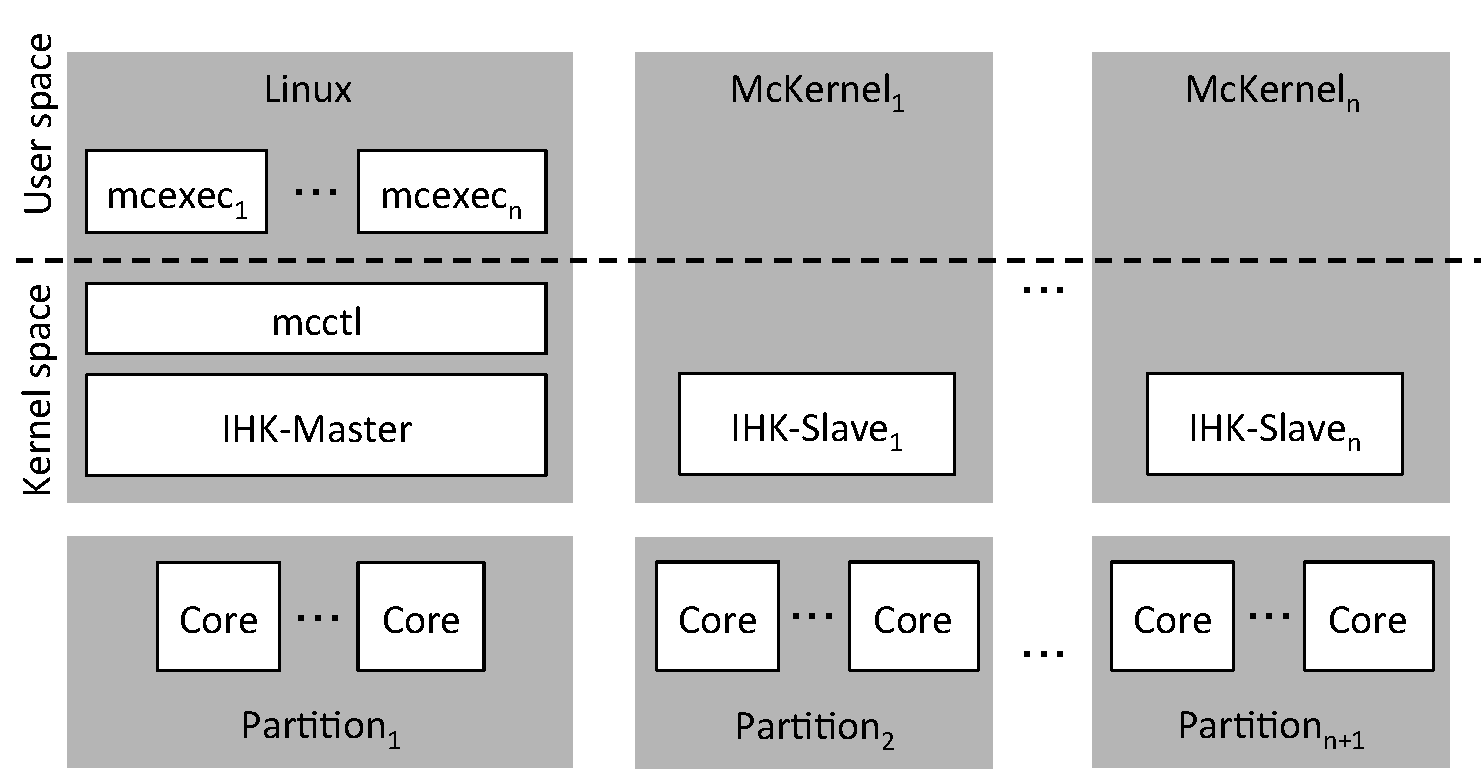
\includegraphics[width=14cm]{figs/arch_overview.pdf}
\vspace{-0em}\caption{The architecture of McKernel}
\label{fig:arch_overview}
\vspace{-0em}
\end{figure}
\FloatBarrier

Two kernel modules,
\texttt{mcctl} and \texttt{IHK-Master}, and user processes
\texttt{mcexec} (\texttt{mcexec1, mcexec2, ...})
exist in the Linux kernel while
McKernel (\texttt{McKernel1, McKernel2, ...}) and 
IHK-Slave (\texttt{IHK-Slave1, IHK-Slave2, ...}) reside
in each partition.

Linux controls all hadware resources when booting a compute-node.
The Interface for Heterogeneous Kernel, formed by both \texttt{IHK-Master}
and \texttt{IHK-Slave}, implements a communication mechanism between
Linux and McKernel, called Inter Kernel Communication (IKC).
In addtion of that, the \texttt{IHK-Master} has an important role,
allocating cores and memory for McKernel, and booting it.
IHK is independently designed from McKernel, and it may be used for other
kernels with Linux.

The \texttt{mcctl} kernel module controls the McKernel.
In order to provide Linux API for applications running on McKernel,
OS service requests not provided by McKernel is delegated to Linux and
performed by Linux.
The \texttt{mcexec} command requests McKernel to launch an application
via IHK.
After the application's invocation,
a \texttt{mcexec} process acts as a proxy or ghost process for the
McKernel process in the sense that Linux system calls delegated
from McKernel via IHK are issued by this process.

In the rest of this section, 
McKernel features, i.e., McKernel usages, process and memory management,
system calls, and the \texttt{procfs/sysfs} file system will be descried.

\begin{figure}[hbt]
\begin{center}
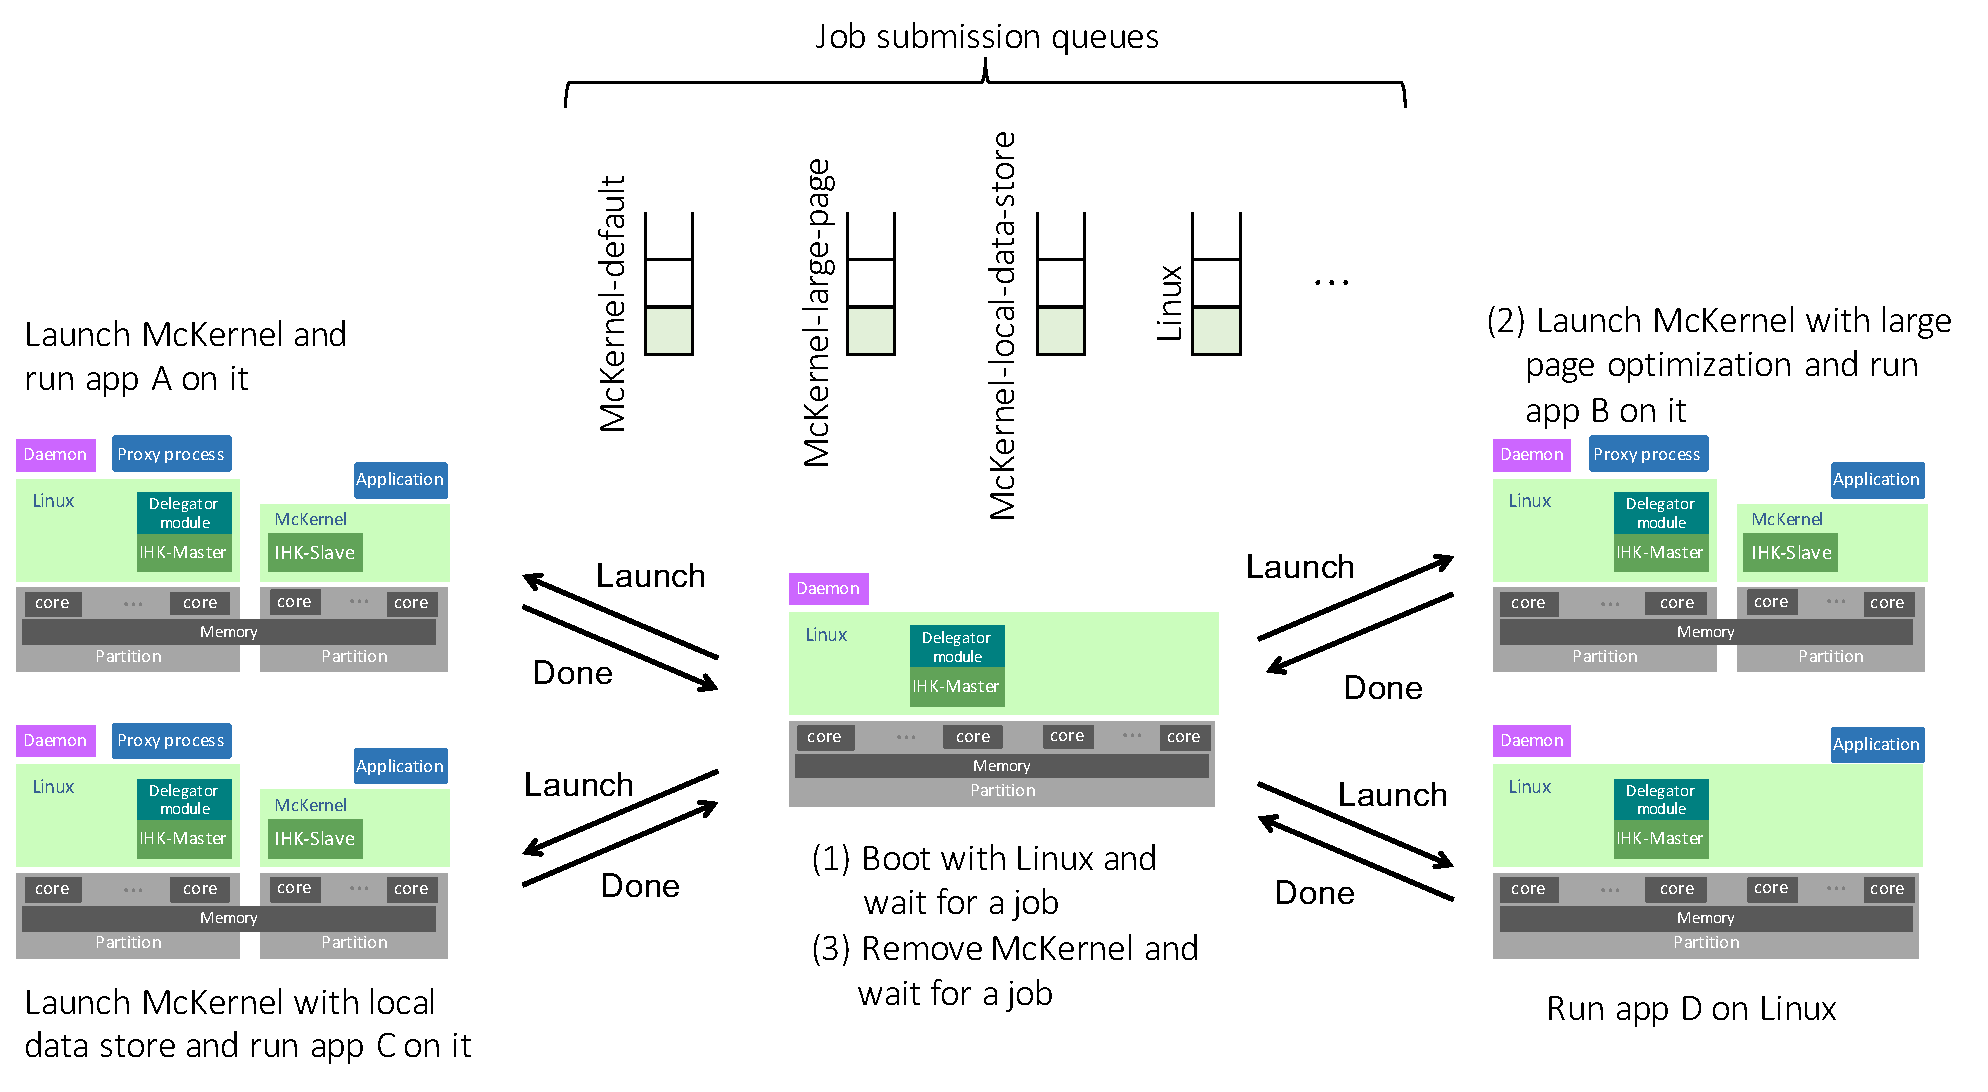
\includegraphics[width=0.9\linewidth]{figs/McKernelUsage.pdf}
\end{center}
\caption{McKernel Usages}\label{fig:mckernel-usage}
\end{figure}
%
McKernelを用いたジョブの実行ステップを図\ref{fig:mckernel-usage}を用いて説明する。
\begin{enumerate}
\item 運用ソフトが計算ノード上にLinuxを起動する(図の(1))
\item ユーザがジョブキューを指定することで、McKernelとLinuxのどちらを使用するか、またMcKernelを使用する場合は様々なチューニングが施されたカーネルイメージのうちどれを使用するかを指定する。例えば、ラージページ化が効果のあるアプリBを実行しようとしている場合は、その機能を持つイメージを指定するジョブキューにジョブを投入する。
\item 運用ソフトウェアがジョブ投入を受けて、資源のパーティショニング、McKernelの起動、アプリの実行を行う(図の(2))。例では、ラージページ化促進機能を持つMcKernelが起動され、アプリBがその上で実行される。
\item 運用ソフトウェアが、ジョブ終了時に計算ノード状態を元の状態、すなわちLinuxのみが動作する状態に戻す(図の(3))
\end{enumerate}

\comment{
Figure \ref{fig:source_mckernel} illustrates the source code tree for
\texttt{mcctl}, \texttt{mcexec}, and McKernel.
%
\begin{figure}[tb]
\centering
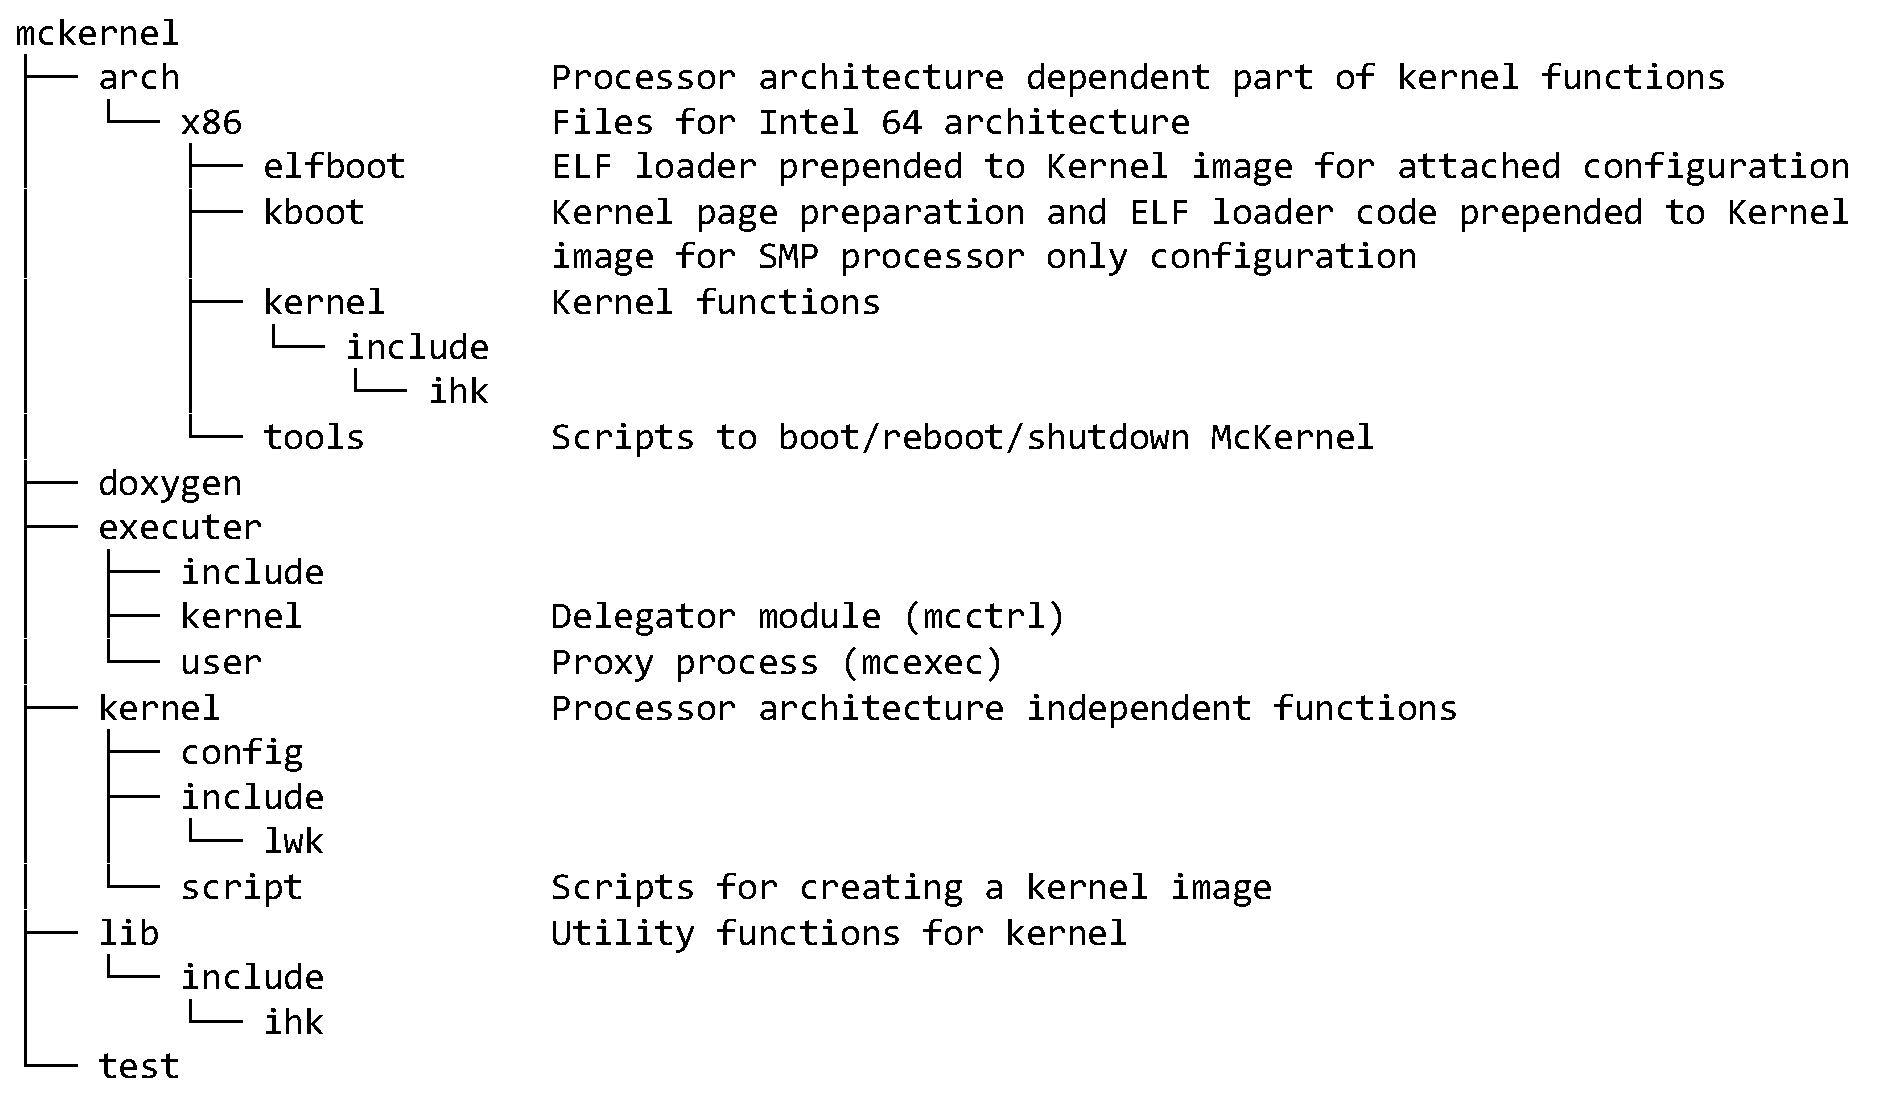
\includegraphics[width=14cm]{figs/source_mckernel.pdf}
\vspace{-0em}\caption{Source Code Tree for \texttt{mcctl}, \texttt{mcexec}, and McKernel}
\label{fig:source_mckernel}
\vspace{-0em}
\end{figure}
\FloatBarrier
}

%%%%%%%%%%%%%%%%%%%%%%%%%%%%%%%%%%%%%%%%%%%%%%%%%%%%%%%%%%%%%%%%%%%%%%%%%%%%%%
\section{\MODAUGS{プロセス管理}}
%%%%%%%%%%%%%%%%%%%%%%%%%%%%%%%%%%%%%%%%%%%%%%%%%%%%%%%%%%%%%%%%%%%%%%%%%%%%%%

McKernel has a unique process execution model to realize cooperation with Linux.
McKernel processes are primarily spawn by the Linux command line
tool \texttt{mcexec}\footnote{An alternative way of creating McKernel processes
via the \texttt{fork()} system call will be discussed in Section \ref{sec:fork}.}.
For every single McKernel process there is a
corresponding \texttt{mcexec} Linux process that exists throughout
the lifetime of the application. \texttt{mcexec} serves the
following purposes:

\begin{itemize}
\item[-] It provides an execution context for offloaded system calls
(explained in Section \ref{sec:syscall_offloading})
so that they can be invoked directly in Linux
\item[-] It enables transparent access to Linux device drivers through the mechanism of unified address-space (discussed in Section \ref{sec:unified_address_space}) and the ability to map Linux device files directly to McKernel processes 
\item[-] It facilitates Linux to maintain certain application associated
kernel state that would have to be otherwise maintained by McKernel
(e.g., open files and the file descriptor table
(see Section \ref{sec:proxy_files}), process specific
device driver state, etc.)
\end{itemize}

Due to its role to providing a gateway to specific Linux features,
we call \texttt{mcexec} the \emph{proxy-process}.
Figure \ref{fig:syscall_offloading} provides an overview of IHK/McKernel's
proxy-process architecture as well as the system call offloading mechanism.
%
\begin{figure}[h!]
\centering
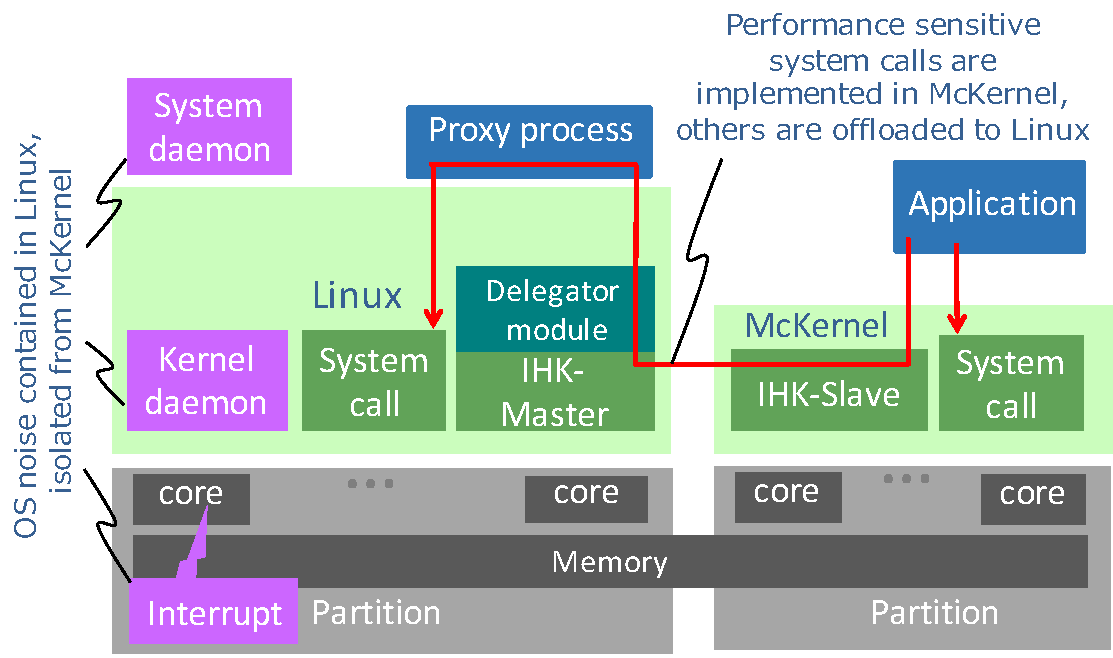
\includegraphics[width=0.82\linewidth]{figs/syscall_offloading.pdf}
\vspace{-0em}\caption{Overview of the IHK/McKernel architecture and
the system call delegation mechanism.}
\label{fig:syscall_offloading}
\vspace{-0em}
\end{figure}
\FloatBarrier

We emphasize that IHK/McKernel runs HPC applications primarily on the LWK
but the full Linux API is available via system call delegation.
System call offloading will be detailed in Section \ref{sec:syscall_offloading}.

Since the user shell process runs on the Linux side, a signal to an
McKernel process cannot be delivered directly from Linux.
Instead, the shell process issues signals to \texttt{mcexec}
and \texttt{mcexec} forwards the signal to the McKernel process
via IKC. For more information on singnaling, see Section \ref{sec:signaling}.

\subsection{Linuxからのプロセス起動}\label{sec:proc_launch}
\texttt{mcexec}がLinuxからプロセスを起動するステップは以下の通り。
\begin{enumerate}
\item It opens the device \texttt{/dev/mcos\textit{n}} to communicate with
McKernel.
\item It sends the ELF binary description header, the commmand line
and environment variables to the McKernel. %(MCEXEC\_UP\_PREPARE\_IMAGE)。
\item It uploads the application binary to McKernel's memory area.
%(MCEXEC\_UP\_TRANSFER)。
\item It creates a Linux thread pool that will serve system call offloading
requests. Additionally, one of the workers is designated for waiting for
signals from McKernel.
\item It sends a request for starting the process to McKernel.
%\\(MCEXEC\_UP\_START\_IMAGE)。
\item The main thread waits for termination of all workers.
\item When a worker receives the \texttt{exit\_group()} system call,
it terminates all workers in the thread pool.
\end{enumerate}

\MODAUG{なお、環境変数\texttt{MCEXEC\_WL}にMcKernel用実行可能ファイルの(親)ディレクトリを指定することで、\texttt{mcexec}の指定を省略できる。複数ディレクトリを指定する場合は、コロンをデリミタとして指定する。なお、指定ディレクトリ以下に実行可能ファイルが存在しても、以下のケースではLinuxで実行される。}
\begin{itemize}
\item \ADDAUG{McKernelが動作していない場合}
\item \ADDAUG{コマンドが64ビットELFバイナリではない場合}
\item \ADDAUG{コマンド名が \texttt{mcexec}, \texttt{ihkosctl}, \texttt{ihkconfig}である場合}
\end{itemize}
\MODAUG{この機能は、\texttt{mcctrl}がLinuxのローダのリストに特別なローダを挿入することで実現される。}
%なお、このローダのリストは複数のバイナリ形式(ELFやスクリプトなど)をサポートするために存在する。
%なお、上記ルールにおいてコマンドのパスは絶対パスで評価する。具体的には\texttt{d\_path()}で絶対パスを求めている。\texttt{symlink()}などのパスでは評価されないため、注意すること。

%=============================================================================
\subsection{\MODAUGS{\texttt{fork()}}}
%=============================================================================
\label{sec:fork}
The \texttt{fork()} system call is supported in McKernel and it is an alternative
way for spawning new processes. \texttt{fork()} is handled as follows:

\begin{enumerate}
\item McKernel allocates a CPU core and memory for the child process.
\item McKernel creates information on process and virtual memory,
and the user execution context.
\item McKernel copies the parent memory to the child process.
\MODAUG{Note that the anonymous memory areas such as text, data, bss, are copied without using copy-on-write technique in the current implementation.}
\item McKernel requests \texttt{mcexec} to perform a fork system call (i.e.,
 to create a new proxy process for the child) in Linux.
 \texttt{mcexec} executes the following steps:
  \begin{enumerate}
  \item \texttt{mcexec} issues the fork system call to create a new Linux
	process (call it the child proxy).
  \item The child proxy closes the device
    \texttt{/dev/mcos\textit{n}} and reopens it again
    in order to communicate with McKernel.
  \item The child proxy creates the worker thread pool that serve the same role
  of the parent process's worker threads.
  \item The child proxy sends a reply message to McKernel.
  %\item \MODAUG{The child proxy calls \texttt{munmap()} to release memory mappings of the original McKernel process.}
  \end{enumerate}
\item \MODAUG{When McKernel receives the reply message, it puts the child process into the run-queue.}
\item McKernel returns to its parent process with the child process ID.
\end{enumerate}

\comment{
%=============================================================================
\subsection{Context Switch}
%=============================================================================
McKernelは標準的な方法でコンテキストスイッチを行う。
ポスト京アーキテクチャではプロセス切替時にTLBフラッシュを必要となる可能性があるため、コンテキストスイッチが頻繁に起こるアプリケーションに対してこのオーバヘッドが大きくなるという課題がある。
この課題に対しては、PVASカーネルとユーザレベルスケジューリングを組み合わせて使用することで対応する。
PVASカーネルでは、複数のユーザプロセスが仮想アドレス空間を共有することができる。
このため、ユーザレベルスケジューラと組み合わせることで、TLBフラッシュを不要とすることができる。

また、コア数を大幅に上回る数のプロセスを動作させるプログラミングモデルが注目を集めている。
このようなプログラムでは、コンテキストスイッチに伴うカーネルモードに移動する際のオーバーヘッドが大きくなるという課題がある。
この課題に対しては、ユーザレベルスケジューリングを使用することで対応する。
}

%=============================================================================
\subsection{Files and the File Descriptor Table}
%=============================================================================
\label{sec:proxy_files}
McKernel does not maintain file system related information (e.g., file caches)
and file descriptors are managed by the proxy process on Linux.
When an McKernel process opens a file, its file descriptor is created
in the \texttt{mcexec} process and the number is merely returned to
the McKernel process.

It is worth noting that \texttt{mcexec} keeps the IHK device file open
for communication with McKernel. Because a file descriptor is an integer value,
the IHK device could theoretically be accessed from application code.
In order to avoid such scenario, \texttt{mcexec} ensures that the IHK device
file cannot be accessed by application code.

%=============================================================================
\subsection{\MODAUGS{Signal Handling}}
%=============================================================================
\label{sec:signaling}
Two types of signals are considered:
One is signals for the \texttt{mcexec} process. An example is
the user sends a signal to the process from the shell.
Another one is signals for a McKernel process, e.g., page fault
signal caused by accessing wrong address in the McKernel process.

When the \texttt{mcexec} process receives a signal, that signal
is transfered to the McKernel process via McKernel.
When McKernel receives a signal for the McKernel process from the
\texttt{mcexec} process during waiting for completion of a Linux
system call, McKernel requests the \texttt{mcexec} process for
aborting the system call execution.

\comment{
\subsubsection{シグナル中継}
McKernelでは\texttt{mcexec}を宛先としたシグナルをMcKernelプロセスに中継する。
こうすることで、ターミナルからの\texttt{Control+C}入力や、MPIプロセスへのシグナル送信を行えるようにする。
}

\comment{
設計方針は以下の通り。
\begin{enumerate}
\item ホストOSで発生したシグナルは、起動コマンド(mcexec)が受け取り、IKC通信を用いてMcKernelにシグナルの発生を通知する。
\item McKernelで発生するシグナルの内、割り込みに基づくものは割り込みハンドラを契機として処理する。具体的にはGeneral Protection Fault(GPF)とPage Faultが該当する。
\item killなどのシステムコール呼び出しに起因するシグナルや、子プロセス終了(SIGCHLD)に起因するシグナルはMcKernel内で処理する。
\item シグナル受信プロセスがreadシステムコールなどの時間が掛かるシステムコールを発行し、その完了待ち状態の可能性があるため、シグナル受信プロセスに対応するmcexec内のスレッドに対してシグナルを送付してシステムコールを中断させる。これは、McKernelからホストOSのmcexecにIKC通信を用いて要求する。
\end{enumerate}

シグナル中継処理の概要を図\ref{fig:signal_flow}に示す。
\begin{figure}[h!]
\centering
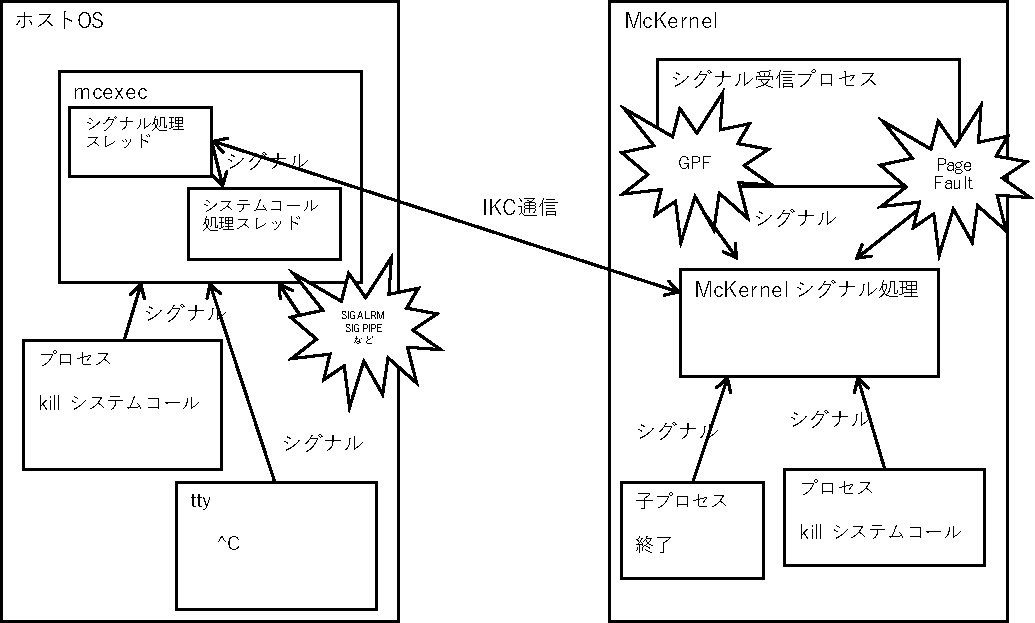
\includegraphics[width=14cm]{figs/signal_flow.pdf}
\vspace{-0em}\caption{シグナル処理の概要}
\label{fig:signal_flow}
\vspace{-0em}
\end{figure}

シグナル処理のサポート範囲は、以下の通り。
\begin{enumerate}
\item ホストOS(mcexec)が受け取ったシグナル
\begin{itemize}
\item 他のプロセスやttyから送られた任意のシグナル
\item mcexec 内部で発生したシグナル(SIGALRMやSIGPIPEなど)
\end{itemize}
\item McKernelで動作するプロセスが発行したシグナル
\begin{itemize}
\item kill系のシステムコール(kill, tkill, tgkill, sigqueue)で送付される任意のシグナル
\item 子プロセス終了時に送付されるシグナル(SIGCHLD)
\end{itemize}
\item McKernelで動作するプロセスで発生した異常
\begin{itemize}
\item General Protection Fault(SIGILL)
\item Page Faultの内、不正なアドレス参照(SIGBUS, SIGSEGV)
\end{itemize}
\end{enumerate}
これらの事象が発生した場合、McKernelで動作するシグナル受信プロセスにシグナルが通知され、処理される。


\subsubsubsection{データ構造}
\subsubsubsection*{process構造体}
process構造体はプロセスとスレッドに関する情報を保持する。process構造体に、シグナル用の情報として以下を持つ。
\begin{verbatim}
struct process {
  ...
  volatile int sigevent;          // シグナル到着フラグ (pauseで使用)
  sigset_t sigmask;               // シグナルマスク
  stack_t sigstack;               // シグナルスタック
  ihk_spinlock_t sigpendinglock;  // sigpending用ロック
  struct list_head sigpending;    // スレッドが受け取ったシグナルのリスト
  struct sig_shared *sigshared;   // プロセスが受け取ったシグナルの管理テーブル
  struct sig_handler *sighandler; // シグナルハンドラ管理テーブル
};
\end{verbatim}

\subsubsubsection*{\texttt{sig\_shared}構造体}
\texttt{sig\_shared}構造体は、プロセスが受け取ったシグナル(処理するプロセス中のスレッドが決定していない)を管理する。\texttt{sig\_shared}構造体の定義は以下の通りである。
\begin{verbatim}
struct sig_shared {
  ihk_spinlock_t lock; // sigpending用ロック
  ihk_atomic_t use;    // 参照カウンタ(削除時に使用)
  struct list_head sigpending;// プロセスが受け取ったシグナルのリスト
};
\end{verbatim}

\subsubsubsection*{\texttt{sig\_pending}構造体}
\texttt{sig\_pending}構造体は、プロセスまたはスレッドが受け取った1つのシグナルを表す。\texttt{sig\_pending}構造体の定義は以下の通りである。
\begin{verbatim}
struct sig_pending {
  struct list_head list; // sig_pendingのリスト
  sigset_t sigmask;      // シグナル処理時のシグナルマスク
  siginfo_t info;        // siginfo構造体
};
\end{verbatim}

\subsubsubsection*{\texttt{sig\_handler}構造体}
\texttt{sig\_handler}構造体は、プロセスのシグナルハンドラ情報を保持する。\texttt{sig\_handler}構造体の定義は以下の通りである。
\begin{verbatim}
struct sig_handler {
  ihk_spinlock_t lock;              // action用ロック
  ihk_atomic_t use;                 // 参照カウンタ(削除時に使用)
  struct k_sigaction action[_NSIG]; // シグナル番号毎のアクション
};
\end{verbatim}
}

図\ref{fig:signal_relay_flow}を用いてシグナル中継機能の動作を説明する。
ホストOSのmcexecが受け取ったシグナルは、IKCを通じてMcKernelに通知され、シグナル登録処理(\texttt{do\_kill})に伝えられる。シグナル登録処理では、シグナルを表す\texttt{sig\_pending}構造体を作成し、シグナル送付先のprocess構造体に登録する。ここで、シグナル送付先がスレッドの場合はprocess構造体の\texttt{sigpending}に登録するが、スレッドを特定しないシグナルの場合はprocess構造体の中のスレッド共通の\texttt{sigshared}の\texttt{sigpending}に登録する。
他の事象により発生したシグナルも同様にシグナル登録処理(\texttt{do\_kill})によってprocess構造体にシグナルが登録される。
\MODAUG{シグナルを受信するプロセスを実行するCPUでは、割り込み処理後やシステムコール処理後などのユーザ空間への切り替えのタイミングでプロセスに届いているシグナル(process構造体に登録されている\texttt{sig\_pending}構造体)をチェック(\texttt{check\_signal})し、シグナルが届いている場合には、その処理を行う。}
シグナルの処理は、process構造体の\texttt{sighandler}に従って行う。\texttt{sighandler}のシグナル番号の項目にシグナルハンドラが登録されている場合は、登録されているシグナルハンドラを呼び出す。シグナルを無視する場合は何もしない。それ以外の場合はプロセスを終了(シグナルによる終了)する(但し、シグナル番号がSIGCHLDとSIGURGでは、シグナルハンドラの登録が無い場合は無視される)。
\begin{figure}[h!]
\centering
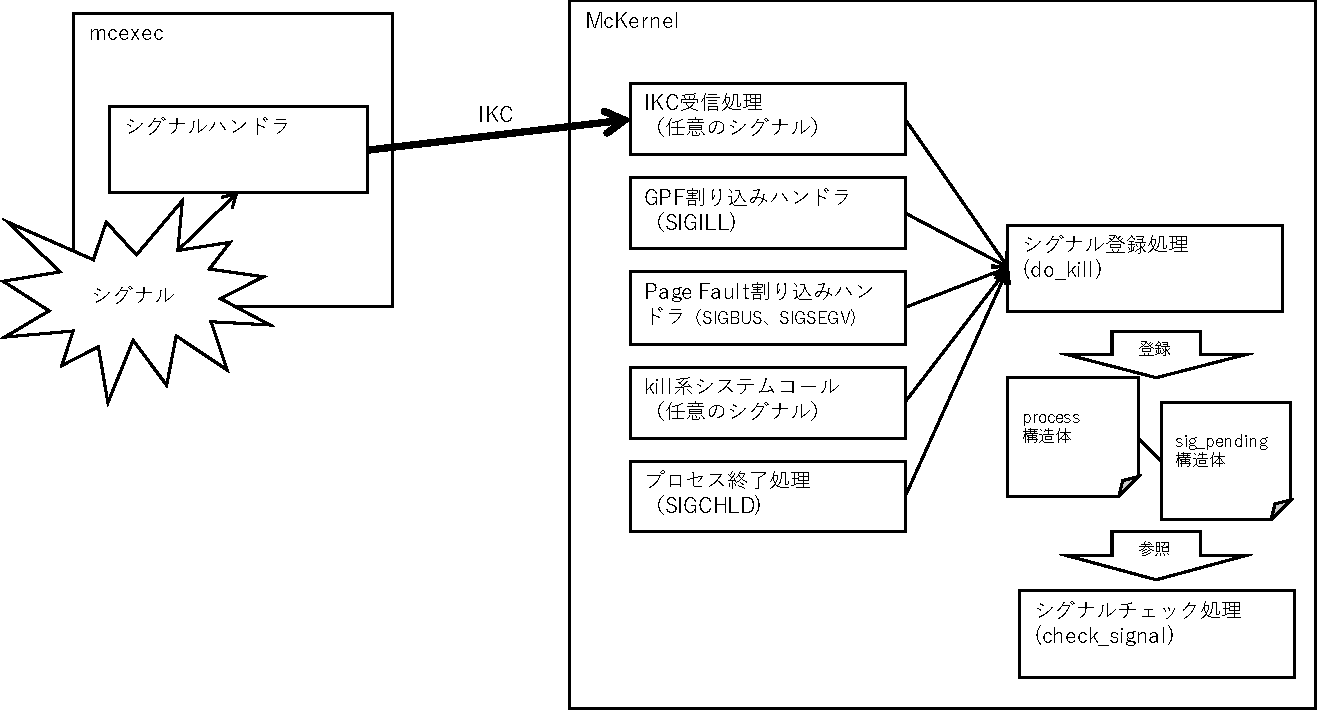
\includegraphics[width=13cm]{figs/signal_relay_flow.pdf}
\vspace{-0em}\caption{シグナル中継処理の動作}
\label{fig:signal_relay_flow}
\vspace{-0em}
\end{figure}
\FloatBarrier


%=============================================================================
\subsection{Process ID}
%=============================================================================
The process ID of a McKernel process is held in the corresponding proxy process and it is managed via Linux API.

\subsection{Thread ID}
McKernelスレッドのスレッドIDは、対応するproxy processスレッドで管理される。
McKernelスレッド生成時のproxy processスレッドとの対応付けステップは以下の通り。
\begin{itemize}
\item[C1] proxy process (\texttt{mcexec})は起動時に生成するスレッド数を決定し、その数だけ生成する。
\item[C2] McKernelはスレッド生成時に、そのスレッドと対応付けるproxy processのスレッドをproxy processに問い合わせる。
\item[C3] McKernelは新しく生成するMcKernelスレッドに当該proxy processスレッドのスレッドIDを割り当てる。また、McKernelはスレッドIDをキャッシュすることでスレッドID問い合わせを高速化する。
\end{itemize}

\texttt{mcexec}は生成するスレッド数を以下の方法で決定する。
\begin{itemize}
\item[S1] \texttt{-t <nr\_threads>}のオプションが指定された場合はその値を用いる。
\item[S2] 上記オプションが指定されなかった場合は、環境変数\texttt{OMP\_NUM\_THREADS}が設定されている場合は、環境変数の値を用いる。この環境変数が設定されていない場合はMcKernelに割り当てられたCPU数を用いる。
\end{itemize}

McKernelのスレッド数上限はproxy processがステップC1で生成するスレッド数で決まる。
このためユーザは上記のステップS2で決定される数では足りない場合は\texttt{mcexec}の\texttt{-t <nr\_threads>}オプションを用いて十分な数を指定する必要がある。


\subsection{\MODAUGS{User ID}}
\MODAUG{UID情報取得のオーバーヘッドを削減するため、UIDはMcKernelとLinuxの両方で管理する。
変更の際はMcKernel上の値を変更した後、IKCを用いてLinux上の値を変更する。}

\subsection{\MODAUGS{Process Groups}}
\MODAUG{プロセスグループにシグナルを送付する際のシグナル送付対象プロセス調査のオーバーヘッドを削減するため、また、\texttt{setpgid}システムコールにおいて、対象プロセスがexecveを実行したか否かのチェックを行えるようにするため、pgidはLinuxとMcKernelの両方で管理する。変更の際はMcKernel上の値を変更した後、IKCを用いてLinux上の値を変更する。}

\comment{
\subsection{\texttt{ptrace()}向けレジスタアクセス機能}
ptraceシステムコールはサブコマンド\texttt{PTRACE\_GETREGS}、\texttt{PTRACE\_SETREGS}によってプロセスのレジスタアクセスする。

設計方針は以下の通り。
McKernelでは,ユーザレジスタは,カーネルモードに遷移したときのスタックフレーム上に退避される。このスタックフレームがそのままユーザコンテクストとなる。そこで,このスタックフレームに,退避・回復を省略しているレジスタ用の領域も確保する。ただし,従来通り,モード遷移時にはこれらのレジスタの退避・回復を省略する。
アーキ依存の新規関数\texttt{lookup\_user\_context}を導入する。この関数は,既存のユーザコンテクストに,退避を省略しているレジスタを追加退避させることで完全なユーザコンテクストを作成し,そのアドレスを返す。\texttt{lookup\_user\_context}関数を介して完全なユーザコンテクストにアクセスさせることで,ptraceシステムコールの処理による必要なレジスタへのアクセスのすべてを実現する。 

\subsubsection{関数仕様}
\subsubsection*{書式}{\quad} \texttt{ihk\_mc\_user\_context\_t *lookup\_user\_context(struct process *proc);}
\begin{funcdef}
\funcarg{proc}{\IN}{対象スレッド}
\end{funcdef}


\texttt{struct x86\_user\_context}は,IA-32eアーキテクチャでの\texttt{ihk\_mc\_user\_context\_t}構造体の実装として以下のように定義される。
\footnotesize
\begin{verbatim}
struct x86_basic_regs {
    unsigned long r15, r14, r13, r12, rbp, rbx, r11, r10;
    unsigned long r9, r8, rax, rcx, rdx, rsi, rdi, error;
    unsigned long rip, cs, rflags, rsp, ss;
};

struct x86_sregs {
    unsigned long fs_base;
    unsigned long gs_base;
    unsigned long ds;
    unsigned long es;
    unsigned long fs;
    unsigned long gs;
};

struct x86_user_context {
    struct x86_sregs sr;

    /* 16-byte boundary here */
    uint8_t is_gpr_valid;       // x86_basic_regsの値が有効かを示すフラグ
    uint8_t is_sr_valid;        // x86_sregsの値が有効かを示すフラグ
    uint8_t spare_flags6;
    uint8_t spare_flags5;
    uint8_t spare_flags4;
    uint8_t spare_flags3;
    uint8_t spare_flags2;
    uint8_t spare_flags1;

    struct x86_basic_regs gpr;
    /* 常に退避するレジスタ群。このフィールドは、カーネルモード遷移時に作成される
       スタックフレームそのものなので,これより後ろにフィールドを置くことはできない */
    /* 16-byte boundary here */
};
typedef struct x86_user_context ihk_mc_user_context_t;
\end{verbatim}
\normalsize

\subsubsection*{説明}{\quad}
動作は以下の通り。
\begin{enumerate}
\item 引数procで指定されたスレッドが停止していることを確認する
\item \texttt{is\_sr\_valid}がFALSEの場合以下の動作を行う。
\begin{enumerate}
\item 指定されたスレッドのユーザコンテクストの\texttt{x86\_sregs}に初期値を格納する
\item \texttt{is\_sr\_valid}をTRUEにする
\end{enumerate}
\item 指定されたスレッドのユーザコンテクストへのポインタを返す
\end{enumerate}

\subsubsection*{戻り値}{\quad}
引数procが示すスレッドの,完全なユーザコンテクストへのポインタ

\subsubsection{制限事項}
本機能を使って取得したユーザコンテクストのうち、\texttt{ds, es, fs, gs, gs\_base}の各レジスタの値は,プロセス開始時の初期値であって実際の値ではない。
また,本機能を使って取得したユーザコンテクストのうち、\texttt{fs\_base, gs\_base, ds, es, fs, gs}の各レジスタの値を書き換えても,ユーザレジスタの値を変更することはできない。

McKernelは,32ビットプロセスをサポートしていないため,\texttt{ds, es, fs, gs}レジスタが本来の役割で使用されることは無い。また,\texttt{fs\_base, gs\_base}は,スレッド初期化時に設定され,通常,その値が変更されることは無い。したがって,これらのレジスタの値がアプリケーションの動作に影響を与えることは無いので,簡易な実装とした。
}

\section{\MODMARS{システムコール}}\label{sec:syscall}
\label{sec:syscall_offloading}

As already mentioned, one of the proxy process' roles is to facilitate system
call offloading by providing an execution context on behalf of the application
so that offloaded calls can be directly invoked in Linux.

%=============================================================================
\subsection{System Call Offloading}
%=============================================================================

The main steps of system call offloading
(also shown in Figure \ref{fig:syscall_offloading}) are as follows.
When McKernel determines that a system call needs to be offloaded
it marshalls the system call number along with its arguments and
sends a message to Linux via a dedicated IKC channel.
The corresponding proxy process running on Linux is by default
waiting for system call requests through an \texttt{ioctl()}
call into IHK's system call delegator kernel module.
The delegator kernel module's IKC interrupt handler wakes up the proxy process,
which returns to userspace and simply invokes the requested system call.
Once it obtains the return value, it instructs the
delegator module to send the result back to McKernel, which subsequently
passes the value to user-space.

System call offloading internally relies on IHK's Inter-Kernel Communication
(IKC) facility. For more information on IKC, refer to ``IHK Specifications''.

%=============================================================================
\subsection{Offloading Strategy}
%=============================================================================
There are mainly two categories of system calls that need
to be implemented by McKernel:

\begin{enumerate}
\item System calls that cannot be offloaded to Linux side, and
\item Performance critical system calls
\end{enumerate}

The first category includes
CPU affinity system calls such as \texttt{sched\_setaffinity()},
signaling system calls such as \texttt{sigaction()},
and memory-related system calls such as \texttt{mmap()} and \texttt{fork()}.
The second category includes timer-related system calls such as
\texttt{gettimeofday()}.

System calls, implemented in McKernel or planned to implement, is
listed in Table \ref{tab:syscalls_implemented}.
Other system calls are delated the Linux.

\begin{table}[!htb]
\centering
\footnotesize
\caption{System calls implemented in McKernel}\vspace{0.0em}
\label{tab:syscalls_implemented}
\begin{tabular}{|p{0.12\linewidth}|p{0.45\linewidth}|p{0.35\linewidth}|} \hline
\multicolumn{1}{|c}{\textbf{Category}}&\multicolumn{1}{|c}{\textbf{Implemented}}&\multicolumn{1}{|c|}{\textbf{Planned}}\\ \hline \hline
Proess management&\texttt{%
arch\_prctl (x86\_64 specific), clone, execve, exit, exit\_group, fork, futex, get\_cpu\_id, gete\{u,g\}id, get\{g,p,t,u\}id, getppid, getres\{g,u\}id, \{get,set\}rlimit, kill, pause, ptrace, rt\_sigaction, rt\_sigpending, rt\_sigprocmask, rt\_sigqueueinfo, rt\_sigreturn, rt\_sigsuspend, set\_tid\_address, setfs\{u,g\}id, set\{g,u,t\}id, setpgid, setre\{g,u\}id, setres\{g,u\}id, sigaltstack, tgkill, vfork, wait4, waittid
}&\texttt{%
\{get,set\}\_thread\_area, rt\_sigtimedwait, signalfd, signalfd4
}\\ \hline
Memory management&\texttt{%
brk, \{get,set\}\_mempolicy, madvise, mincore, mlock, mmap, move\_pages, mprotect, mremap, msync, munlock, munmap, process\_vm\_\{readv,writev\}, remap\_file\_pages, shmat, shmctl, shmdt, shmget
}&\texttt{%
\{get,set\}\_robust\_list, mbind, migrate\_pages, mlockall, modify\_ldt, munlockall
}\\ \hline
Schedule&\texttt{%
getcpu, \{get,set\}itimer, \{get,set\}timeofday, nanosleep, sched\_\{get,set\}affinity, sched\_yield, times
}&\texttt{%
}\\ \hline
Performance counter&\texttt{%
perf\_event\_open
}&\texttt{%
}\\ \hline
\end{tabular}
\vspace{-0em}
\end{table}
\FloatBarrier

%=============================================================================
\subsection{\texttt{gettimeofday()}}
%=============================================================================
\texttt{gettimeofday()} is implemented in user-space by using Virtual Dynamic Shared Object (vDSO) mechanism (see Section \ref{sec:vdso} for vDSO).
).

Table \ref{tab:vdso_gettimeofday} shows the related vDSO pages.
\begin{table}[!ht]
\centering
\footnotesize
\caption{vDSO pages related to \texttt{gettimeofday()}}\vspace{0.0em}
\label{tab:vdso_gettimeofday}
\begin{tabular}{|p{0.20\linewidth}|p{0.66\linewidth}|} \hline
\multicolumn{1}{|c}{\textbf{Name}}&\multicolumn{1}{|c|}{\textbf{Description}}\\ \hline \hline
\texttt{vdso}&System call code and data\\ \hline
\texttt{vvar}&Kernel variables\\ \hline
\texttt{hpet}&Rregister of the High Precision Event Timer\\ \hline
\texttt{pvti}&Virtual clock updated by virtual machine, such as Xen and KVM\\ \hline 
\end{tabular}
\vspace{-0em}
\end{table}
\FloatBarrier

\subsection{\texttt{perf\_event\_open()}}
\texttt{perf\_event\_open()} is implemented in McKernel by using the technique mentioned in Section \ref{sec:mckfd}.

\comment{
\subsection{ptrace向け他プロセス空間書き込み機能}
ptraceシステムコールに他プロセス空間書き込み機能を提供することを目的とする。
該当するptraceのサブコマンドは\texttt{PTRACE\_POKETEXT}である。

書き換え範囲を含むページの共有を解除してから、対象物理ページを直接書き換える方針とする。
書き換え範囲内のページ共有の解除は,書き換え範囲全体に特別なページフォルト (\texttt{PF\_PATCH}) 処理を実行することで実現する。\texttt{PF\_PATCH}処理は,書き込み可能な属性のページに対しては,storeによるページフォルトと同じ処理 (\texttt{PF\_POPULATE}) を実行する。一方,書き込みできないページに対しては,対応する物理ページを得られる時に限って,新規に割り当てたページにデータをコピーしてページを入れ替えることで,他のマッピングとのページ共有を解除する。なお,例えば誰もアクセスしていない\texttt{PROT\_NONE}マッピングのような,書き込みできないページであって,対応する物理ページも得られない場合は,\texttt{PF\_PATCH}処理であってもEACCESエラーで失敗する。
物理ページの書き換えは,カーネル仮想空間上のストレートマッピング領域を介しておこなう。これは,\texttt{PTRACE\_POKETEXT}動作で書き換えるページの書き込み可否属性を,\texttt{PTRACE\_POKETEXT}前後で変えないようにするためである。

\subsubsubsection{関数仕様}
\subsubsection*{書式}{\quad} \texttt{int patch\_process\_vm(struct process\_vm *vm, void *udest, const void *ksrc, size\_t size)}
\begin{funcdef}
\funcarg{vm}{\IN}{書き込まれるプロセス空間}
\funcarg{udest}{\IN}{書き込み開始ユーザアドレス}
\funcarg{ksrc}{\IN}{書き込むデータの先頭のカーネルアドレス}
\funcarg{size}{\IN}{書き込むサイズ}
\end{funcdef}

\subsubsection*{説明}{\quad}
動作は以下の通り。
\begin{enumerate}
\item フォルトアドレスに対応する仮想ページを特定する
\item 仮想ページが属する\texttt{vm\_range}の属性が\texttt{PROT\_NONE}の場合以下のように動作する。
\begin{enumerate}
\item 物理ページが割り当てられているか確認し、割り当てられていない場合はEACCESを返しエラー終了する
\item 物理ページがmemobjに属するページか,他プロセスにマップされているページであった場合は、新規に割り当てたページにデータをコピーし,ページを入れ替える
\item ゼロを返す
\end{enumerate}
\item 仮想ページが属する\texttt{vm\_range}の属性が\texttt{PROT\_NONE}以外で,かつ,\texttt{PROT\_WRITE}がない場合以下のように動作する。
\begin{enumerate}
\item \texttt{PF\_POPULATE}処理をして物理ページの存在を保証する
\item 物理ページがmemobjに属するページか,他プロセスにマップされているページであった場合は、新規に割り当てたページにデータをコピーし,ページを入れ替える
\item ゼロを返す。
\end{enumerate}
\item 仮想ページが属する\texttt{vm\_range}の属性に\texttt{PROT\_WRITE}がある場合以下のように動作する。
\begin{enumerate}
\item \texttt{PF\_POPULATE}処理をして物理ページの存在を保証する
\item ゼロを返す
\end{enumerate}
\end{enumerate}

\texttt{patch\_process\_vm()}は,1ページずつ処理をするため,書き換える領域を大きくしても性能が向上することは無い。ptraceシステムコールで複数ページに及ぶような書き換えをおこなうことはまれなので,このことが実際に性能問題を起こすことは無い。
\texttt{patch\_process\_vm()}は,相手プロセスが停止していないと正しく動作しない。これは,書き換え時に自プロセスの空間でページフォルトが発生する可能性があるため,相手空間のロックを確保し続けることができないからである。相手空間のロックを確保しつづけてしまうと,互いに相手空間の書き換えを試みた時にデッドロックする可能性がある。ptraceシステムコールの\texttt{PTRACE\_POKETEXT}動作および\texttt{PTRACE\_POKEDATA}動作は,相手プロセスが停止している場合のみ書き換えを実行するので,このことが問題となることは無い。

\subsubsection*{戻り値} 
\begin{table}[!ht]
\footnotesize
\begin{tabular}{|p{0.20\linewidth}|p{0.66\linewidth}|} \hline
0&正常終了\\ \hline
0以外&エラー\\ \hline
\end{tabular}
\vspace{-0em}
\end{table}
\FloatBarrier
}

\comment{
\subsection{msync}
McKernelのファイルをバックエンドとするマップへの変更を、Linuxのファイルマップを経由してファイルに伝達することを目的とする。
McKernelは,ファイルIO機能を持たす,ホストOSに処理を委譲している。したがって,あるファイルをmmapでマップしたとき,マップへの変更はMcKernel上のmemobjにバッファされるのに対して,ファイルIOはホストOS上の例えばページキャッシュにバッファされる。このため,マップ上のデータを変更しただけでは,ファイルIOに変更が反映されない。このため、変更のLinuxへの伝達が必要となる。

設計方針は以下の通り。
指定された範囲内のPTEを走査することでmsync動作をする。
msync対象ページの\texttt{PTATTR\_DIRTY}をクリアしてからページIOを実行することによって,ページへの書き込みとmsyncとが競合しても,ページへの書き込み後にページIOが少なくとも1回実行されることを保証する。

動作は以下の通り。
\begin{enumerate}
\item 引数の形式チェック
\item 指定された範囲と重なりを持つ\texttt{vm\_range}構造体について以下を行う。
\begin{enumerate}
\item \texttt{vm\_range}の属性をチェック
\item 指定された範囲と重なりを持つPTEについて以下を行う
\end{enumerate}
\item 引数flagsに\texttt{MS\_SYNC}か\texttt{MS\_ASYNC}があり,PTEがdirtyな場合以下を行う。
\begin{enumerate}
\item PTEをcleanにする
\item ページのデータをファイルに書き戻す
\end{enumerate}
\item 引数flagsに\texttt{MS\_INVALIDATE}があり,PTEがpresentな場合以下を行う。
\begin{enumerate}
\item PTEをクリアしてnot presentにする
\item PTEが示していた物理ページをmemobjから解放する
\end{enumerate}
\item ゼロを返す。
\end{enumerate}
}

\comment{
\subsubsection{制限事項}
msyncを発行したプロセス以外のプロセスによるマップへの変更が書き戻されないことがある。
また,
msyncの本来の動作は,指定された範囲内の物理ページに任意のプロセスによる変更がある場合に,その変更をファイルに書き戻すことである。しかし,あるプロセスのシステムコール処理での他のプロセスの空間の操作は,安易におこなうと他プロセスの性能に悪影響を及ぼすことになる。一方,設計段階ではforkシステムコールやexecveシステムコールの実装が途中のため十分な検討ができない恐れがあった。
そこで,msyncを発行したプロセスによるマップへの変更のみを書き戻す方式を採用した。実際のユーザプログラムでのmsyncの使用では,マップへの変更をしたプロセスがmsyncを発行することがほとんどなので,実用上は問題無いと考える。
msyncで指定された範囲内のページが他のマッピングで共有されている時,\texttt{MS\_INVALIDATE}処理が実行されないことがある。
上記,マップへの変更が書き戻されないことがある問題と同じ理由である。
1ページずつmsync処理を実行するため,大きな範囲を指定しても性能が向上することは無い。
}

\section{Memory Management}
\label{sec:unified_address_space}

We already described how system call offloading works in the IHK/McKernel
architecture.
Notice, however, that certain system call arguments may be pointers
(e.g., the buffer argument of a \texttt{read()} system call) and the actual
operation takes place on the contents of the referred memory.
Thus, the main problem is how the proxy process on Linux
can resolve virtual addresses in arguments so that it can access
the memory of the application running on McKernel.

In order to overcome this problem McKernel deploys a mechanism called
\textit{unified address space}, which essentially ensures that the proxy
process can transparently access the same mappings as its corresponding
McKernel process. This mechanism is detailed in the following sections.

%=============================================================================
\subsection{Unified Address Space}
%=============================================================================
The unified address space model in IHK/McKernel ensures that offloaded system
calls can seamlessly resolve arguments even in case of pointers.
This mechanism is depicted in Figure \ref{fig:unified_address_space}
and it is implemented as follows.
First, the proxy process is compiled as a position independent binary,
which enables us to map the code and data segments specific to the
proxy process to an address range which is explicitly excluded from
McKernel's user space.
The box on the right side of the figure with label "Not used"
demonstrates the excluded region.
Second, the entire valid virtual address range of McKernel's
application user-space
is covered by a special mapping in the proxy process for which
we use a pseudo file mapping in Linux. This mapping is indicated
by the yellow box on the left side of the figure.

\begin{figure}[h!]
\centering
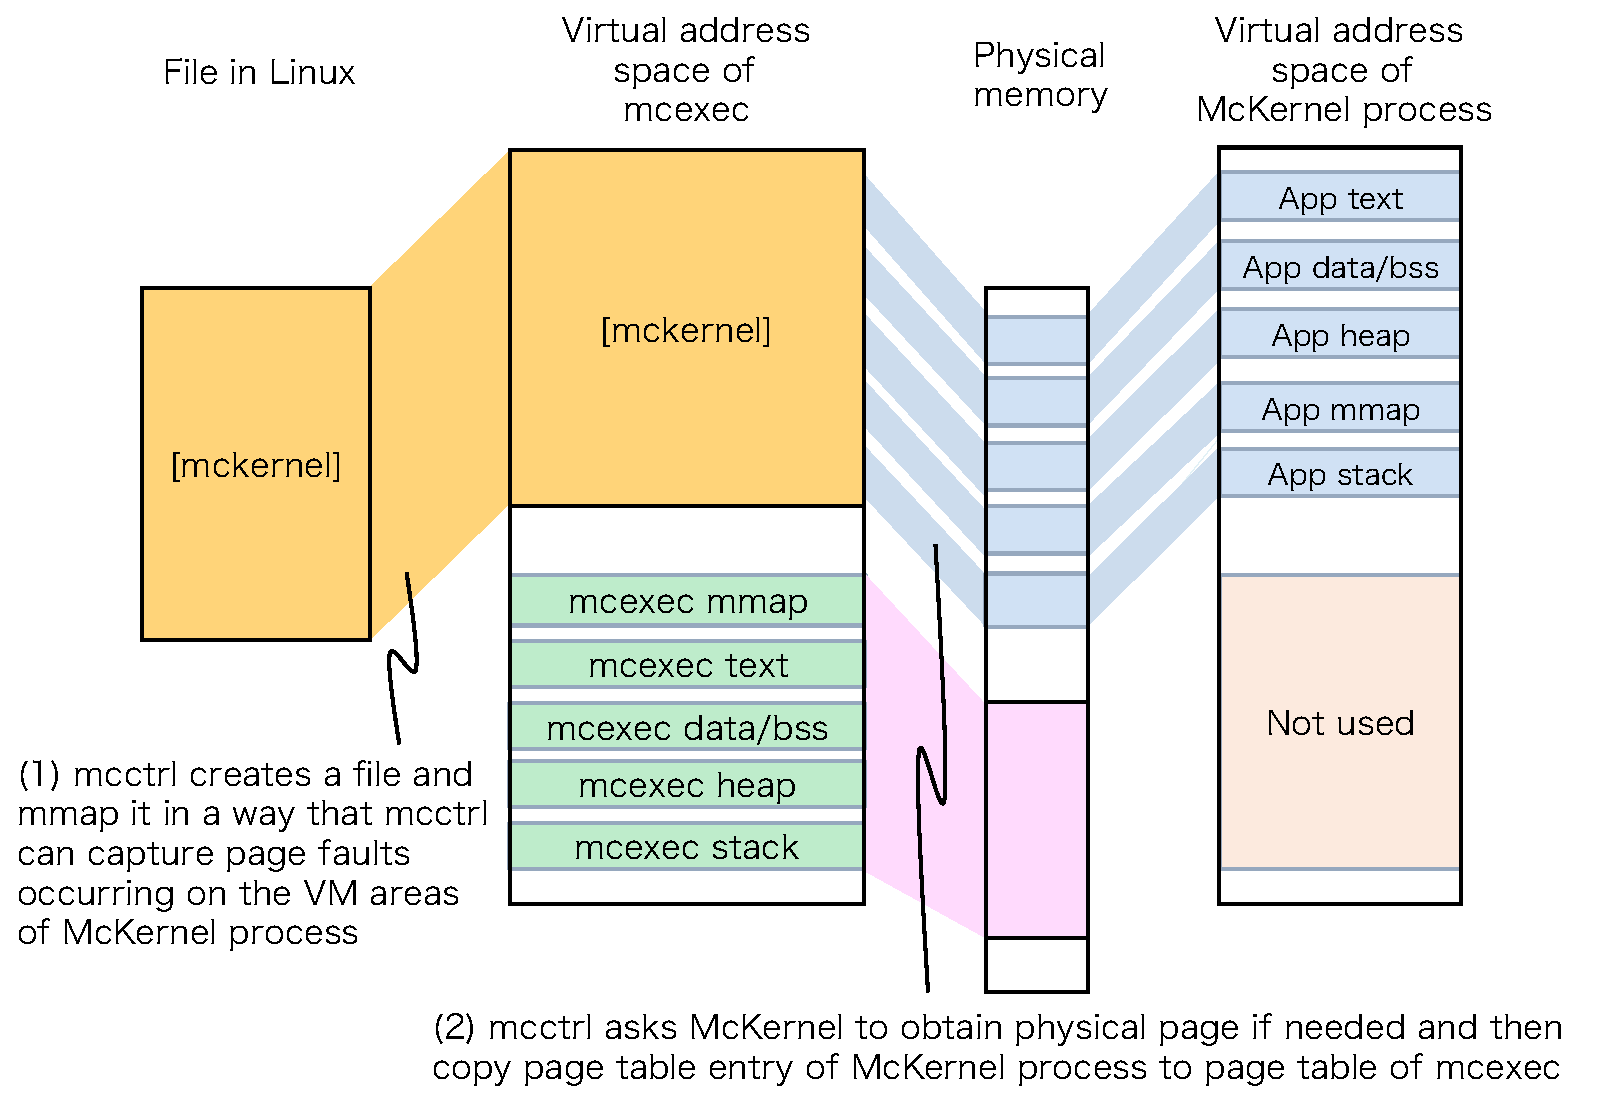
\includegraphics[width=14cm]{figs/unified_address_space.pdf}
\vspace{-0em}\caption{Unified Address Space}
\label{fig:unified_address_space}
\vspace{-0em}
\end{figure}

Note, that the proxy process does not need to fill in any virtual
to physical mappings at the time of creating the pseudo mapping and it
remains empty unless an address is referenced.
Every time an unmapped address is accessed, however, the page fault
handler of the pseudo mapping consults the page tables corresponding
to the application on
the LWK and maps it to the exact same physical page.
Such mappings are demonstrated in the figure by the small boxes
on the left labeled as \textit{faulted page}.
This mechanism
ensures that the proxy process, while executing system calls,
has access to the same memory content as the application.
Needless to say, Linux' page table entries in the pseudo mapping
have to be occasionally
synchronized with McKernel,
for instance, when the application
calls \texttt{munmap()} or modifies certain mappings.

A more detailed sequence of resolving a page fault in Linux for an address
in the McKernel process is as follows:

\begin{enumerate}
\item When \texttt{mcexec} accesses a memory area pointed by
a pointer variable stored in a system call request a Linux
page fault occurs.

\item The \texttt{mcctrl} kernel module captures this page fault.
It looks up the page table of the Mckernel process to find out the page
table entry (PTE) of the physical memory.

\item In case that PTE is not found, the following sequences of issuing
remote page fault are performed as follows.
\begin{enumerate}
\item The \texttt{mcctrl} module interrupts the sytem call service.
It reports return code \texttt{STATUS\_PAGE\_FAULT} and the faulting
address to McKernel.

\item When McKernel receives the return code \texttt{STATUS\_PAGE\_FAULT},
it resolves the page fault.

\item After McKernel finishes page fault processing,
it requests resuming the previous system call process by sending an IKC message
\texttt{SCD\_MSG\_SYSCALL\_ONESIDE} to \texttt{mcctrl}.

\item When \texttt{mcctrl} receives the request of resuming the previous
system call at the IKC message \texttt{SCD\_MSG\_SYSCALL\_ONESIDE},
it looks up the page table entry again.
\end{enumerate}

\item \texttt{mcctrl} maps the physical memory pointed by the PTE
to the virtual address where the page fault occured.

\item \texttt{mcctrl} requests resuming the execution of the \texttt{mcexec}
process.

\item The {\tt mcexec} process now can access the virtual address
requested in the system call.
\end{enumerate}

As mentioned above when an McKernel process releases physical pages by
issuing system calls such as \texttt{munmap()} or \texttt{madvise()} with
the option \texttt{MADV\_REMOVE}, the \texttt{mcexec} process clears
its page tables to make sure future requests will not resolve an
invalid mapping.

When the \texttt{mcexec} process establishes the pseudo mapping covering
the McKernel process's user space the mapping is read/write enabled
except for the text area of the McKernel process.
When the McKernel process allocates a read-only memory mapping,
e.g., when mapping a shared library,
the \texttt{mcctrl} kernel module remaps this area with the same
access permissions in the Linux side.
This remap operation is required because the virtual address sapce
for the McKernel process has been created as one contiguus region
whose access permission is homogeneous.
Most of memory mappings created by the McKernel process are
read/write permission, and thus such remap operation happens
relatively rarely.

%The copy-on-write feature can be implemented in McKernel, but its
%overhead is high because McKernel communicates with \texttt{mcexec}
%every time write-acess fault occurs.          ???????????
%Thus, is has not been implemented in the current McKernel.

%----------------------------------------------------------------------------
\subsubsection{McKernel Process Virtual Address Mapping}
%----------------------------------------------------------------------------
Theoretically all virtual addresses used in the McKernel process must be
mapped to the \texttt{mcexec} process's virtual address.
There are two issues as follows:

\begin{enumerate}
\item The \texttt{mcexec} process has its own text, data and BSS area
whose addresses are also used in the McKernel process if those execution
binaries have been created in the same way.
\item If the huge stack area is allocated to \texttt{mcexec} via shell environment
variable \texttt{RLIMIT\_STACK}, the virtual address space for the McKernel
process cannot be assigned.
\end{enumerate}

The solution of those issues on Linux for x86\_64 architectues is
described as follows.
%,,,,,,,,,,,,,,,,,,,,,,,,,,,,,,,,,,,,,,,,,,,,,,,,,,,,,,,,,,,,,,,,,,,,,,,,,
\subsubsubsection{Avoiding Conflict of text, data, and BSS}
%````````````````````````````````````````````````````````````````````````
In the Linux convention for x86\_64 architectures,
the text segment starts from virtual address 0x400000 and
the data segment starts from 2 MiB upper address than the text segment.
If both an McKernel application and \texttt{mcexec} are compiled and linked,
those addresses are conflict.

As we briefly mentioned above, the \texttt{mcexec} binary is created as
position independent binary
so that each segement's address can be dynamically decided by the runtime.
In Linux convention for x86\_64 architectures, by issuing mmap, the map address
will be the next to the address of the stack area whose address is the highest
address in the user address space.

%,,,,,,,,,,,,,,,,,,,,,,,,,,,,,,,,,,,,,,,,,,,,,,,,,,,,,,,,,,,,,,,,,,,,,,,,,
\subsubsubsection{Huge Stack Size}
%````````````````````````````````````````````````````````````````````````
The virtual address space plan of the McKernel process follows Linux
address plan, i.e., the user space is contiguos and starts from
virtual address 0.
That is, in order to keep the same address space of the McKernel process
in the \texttt{mcexec}, the same address space must not be occupied by
the \texttt{mcexec} process.
There is one problem to do so.
In Linux for x86\_64 architectures,
the start address of a stack area is randomly decided and its
size is the lesser of $\frac{5}{6}$ total memory size and size
specified by the \texttt{RLIMIT\_STACK} environment variable.
If the huge stack occupies the virtual meory in the \texttt{mcexec},
there is no chance to reserve the address space for the McKernel process.
In order to eliminate this problem,
the \texttt{RLIMIT\_STACK} environmental variable for \texttt{mcexec} and
the McKernel process is separeted.
That is, the \texttt{mcexec} checks if \texttt{RLIMIT\_STACK} is
larger than some amount of size (currently 1 GiB),
it saves \texttt{RLIMIT\_STACK} to a temporal environmental variable (\texttt{MCKERNEL\_RLIMIT\_STACK}) and \texttt{exec()} itself again with a small stack (10 MiB).
The new \texttt{mcexec} process restores the original value to \texttt{RLIMIT\_STACK}
so that this environment variable
is used for the McKernel process.


%It should be noted that the reason of 1 GiB maximum stack size for
%\texttt{mcexec} is to keep this virtual address space for checking
%%stack overflow.

%==============================================================================
\subsection{Physical Pages requiring Linux Management}
%==============================================================================
The physical pages of a McKernel process must be under Linux management for I/O related operation (e.g. pin-down).
This is because the driver running on the Linux side performs I/O operation and the operation relies on the Linux paging mechanism.
For example, when a McKernel process tries to send data in a buffer to a remote host,
it calls the Linux driver code and the driver code in turn pins down the physical pages for the buffer using the Linux kernel function.
The kernel function in turn assumes that the pages are under Linux management (i.e. managed by \texttt{struct page}).

Thus, IHK takes the physical pages from physical pages managed by the Linux.
That is, IHK reserves physical pages for the co-kernels
by using \texttt{\_\_get\_free\_pages()} Linux API.
Since the \texttt{\_\_get\_free\_pages()} allocates up to 1024 pages
at a time, IHK repeaditly calls this function to get
contiguous pages more than 1024 pages.

%==============================================================================
\subsection{Handling Different Page Sizes}
%==============================================================================

There are several implementation options to support different page sizes
in Linux:
\begin{enumerate}
\item Linux Transparent Huge Pages (THP)
\item Hugepage option in System V IPC shared memory
\item Linux HugeTLBfs
\item Hugepage option in \texttt{mmap()} flags
\end{enumerate}

McKernel implments a similar technique to Linux THP,
i.e., it automatically maps physical memory with large pages whenever it is
possible.

\subsection{\MODAUGS{\texttt{brk()}}}
\MODAUG{McKernelの\texttt{brk()}システムコールには、ページフォールトオーバーヘッドを削減し、またラージページ化を促進する機能が追加されている。}

\texttt{brk()}の動作は以下の通り。なお、ヒープ終端アドレスを$b$、\texttt{brk()}の引数をページ境界で丸め上げたアドレスを$r$で表す。また、プロセス起動コマンド\texttt{mcexec}(第\ref{sec:mcexec}参照)のオプション(\textttw{--extend-heap-by=<step>})で指定されたパラメタを$S$で表す。
\begin{enumerate}
\item ヒープの縮小が要求された場合、何もせずに戻る。
\item $r-b<S$の場合、ヒープ終端アドレスを以下の$x$に設定する。
$$
r+S{\leq}x<r+S+a, x \bmod a = 0,
a = \left\{ 
\begin{array}{ll}
2^{12} & \mbox{if $S \leq 4096$};\\
2^{21} & \mbox{if $S > 4096$}.
\end{array}
\right.$$
\item $r-b{\geq}S$の場合、ヒープの最終アドレスを$r$に設定する。
\item 拡張された部分をプリページングする。
\end{enumerate}

\MODAUG{なお、この機能は、同一計算ノード上に他ユーザのジョブが存在することはないので、物理ページ利用のフェアネスを考慮する必要がないため、不要になった物理ページをOSに返す必要がない、というHPCアプリの特性を用いている。}

\subsection{\MODAUGS{メモリ割り当てにおけるNUMAノード選択}}
\subsubsection{\MODAUGS{ユーザメモリ割り当て}}
\MODAUG{ユーザメモリ割り当てにおけるNUMAノード選択については、Linuxの機能に対し以下の機能が追加されている。}
\begin{enumerate}
\item ヒープ、anonymous mmap領域だけではなく、text, data, bss, stackの各領域に対してもプロセスのメモリポリシーを用いる。また、これらの領域ごとにプロセスのメモリポリシーを用いるか否かを指定できる。この指定は、プロセス起動コマンド\texttt{mcexec}(第\ref{sec:mcexec}参照)のオプション(\texttt{--mpol-no-\{heap,stack,bss\}})によって行う。
\item ユーザ指定のメモリポリシーを用いるメモリ要求サイズの閾値(この値と同じか大きい場合のみユーザ指定のメモリポリシーを用いる)を指定できる。この指定は、プロセス起動コマンド\texttt{mcexec}(第\ref{sec:mcexec}参照)のオプション(\textttw{--mpol-threshold=<min>})によって行う。
\end{enumerate}

\subsubsection{\MODAUGS{カーネルメモリ割り当て}}
\MODAUG{カーネルメモリ割り当てにおけるNUMAノード選択はLinuxと同様の方法で行う。}
すなわち、NUMAノード間の距離行列を用いて、要求元が存在するNUMAノードから最も距離の短いNUMAノードからメモリを取得する。

\comment{\subsubsection{\ADDAUGS{実装の制限}}
\ADDAUGS{\texttt{mbind()}によるアドレス範囲ごとのメモリポリシー指定はサポートしない。}
}
%=============================================================================
\subsection{Virtual Dynamic Shared Object (vDSO)}
%=============================================================================
\label{sec:vdso}
Mckernel provides the vDSO mechanism, which eliminates the need for switching to kernel-mode when peforming some system calls.

The steps are in the followings.
\begin{enumerate}
\item The physical addresses of the Linux vDSO pages are compiled by looking into \texttt{System.map} when configureing McKernel. They are kept in \texttt{mcctrl}.
\item McKernel adds mappings of the Linux vDSO pages to a process when creating the process. McKernel asks \texttt{mcctrl} for their physical addresses. 
\item McKernel passes their virtual addresses to the process via the Auxiliary Vector in the stack.
\item When a system call is called, first the control is transferred to the \texttt{glibc} wrapper function. And then the control is transferred to the function in the vDSO pages without switching processor mode.
\item The function performs required processing using the data in the vDSO pages.
\end{enumerate}

\comment{
\subsection{Process-in-Process (PiP)}
McKernelはProcess-in-Process (PiP)と呼ばれるメモリ共有ライブラリをサポートする。
%この機能はランタイムライブラリによって透過的にユーザに提供される。例えば、PiPを用いるように修正したMPIライブラリによって提供される。
PiPでは複数タスクが一つの仮想アドレス空間を共有する。
PiPでは、root taskと呼ばれるプロセスの仮想アドレス空間の中に、子タスク(PiP taskと呼ぶ)のメモリ領域を割り当てる。
こうすることで、あるPiP taskは兄弟関係にある他PiP taskのページを読み書きすることができるようになる。

PiPによる仮想アドレス空間共有の様子を図\ref{fig:pip_addr_space}を用いて説明する。
2つのPiPタスクTask\#0、Task\#1が一つの仮想アドレス空間を共有しているとする。
この場合、図のようにTask\#0とTask\#1のtext、data、BSS、stackの各領域およびTask\#0とTask\#1に動的リンクされる共有オブジェクトのtext、data、BSSの各領域は、Root taskのmmap領域に位置する。
%
\begin{figure}[!htb]
\centering
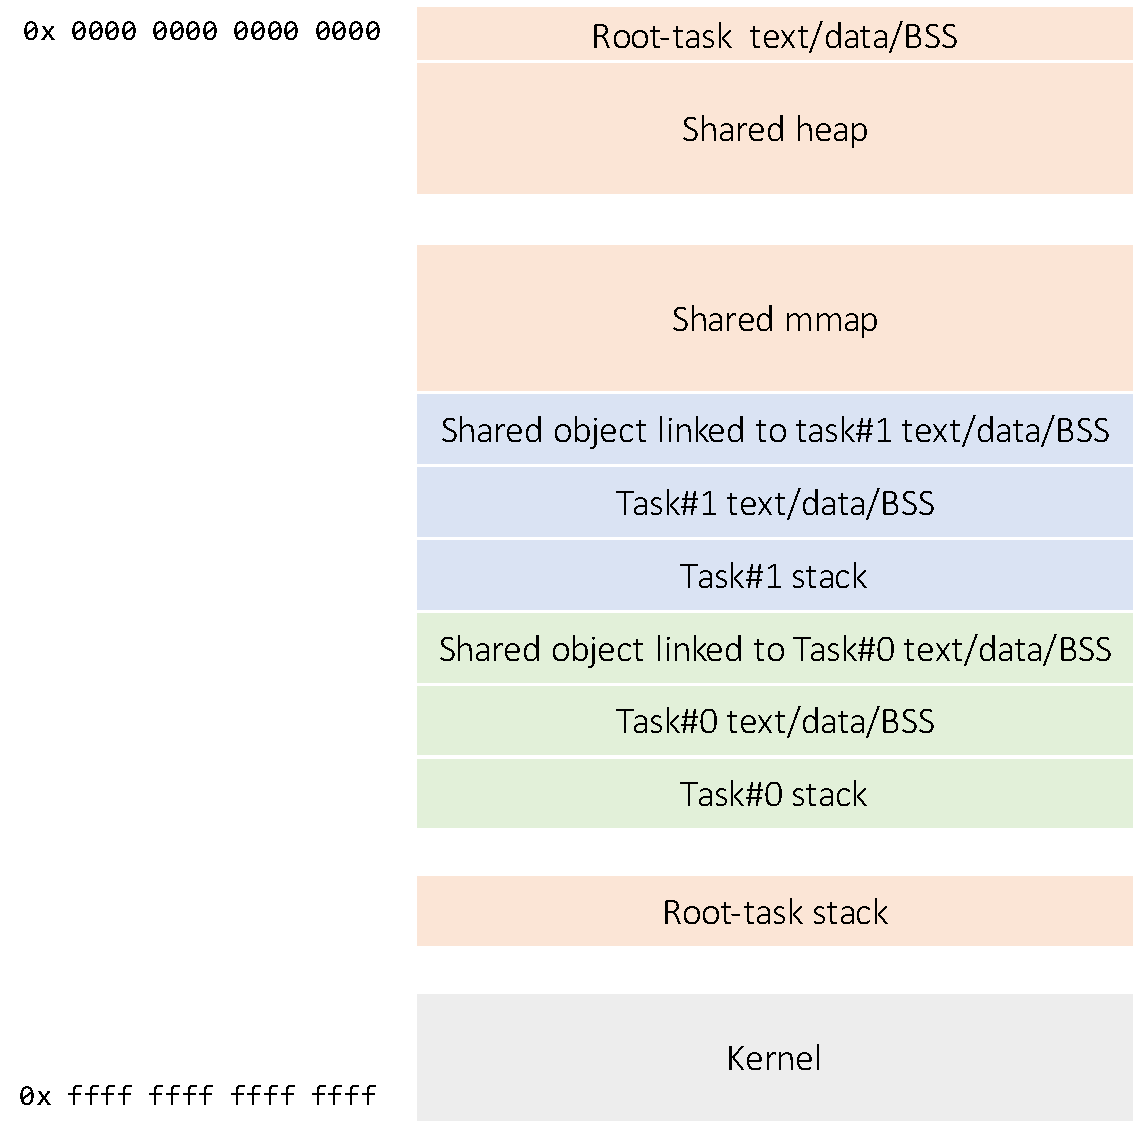
\includegraphics[width=8cm]{figs/pip_addr_space.pdf}
\vspace{-0em}\caption{PiPのメモリマップ例}
\label{fig:pip_addr_space}
\vspace{-0em}
\end{figure}
%
\FloatBarrier
}

\subsection{\ADDAUGS{ファイルマップ}}
ファイルマップはファイルと一対一対応する\texttt{fileobj}と呼ぶ構造体で管理する。
ファイルマップに伴うファイルI/Oは、\texttt{fileobj}と一対一対応する、Linux側に存在する\texttt{pager}と呼ぶ構造体で管理する。
ファイルマップの動作を例を用いて説明する。
\begin{enumerate}
\item 第1のプロセスが\texttt{open()}でファイルディスクリプタを取得する。
\item 第1のプロセスが前記ファイルディスクリプタを引数とした\texttt{mmap()}でMcKernelにファイルマップ作成を要求する。
\item McKernelは\texttt{mcctrl}に\texttt{pager}を要求する。
\item \texttt{mcctrl}は\texttt{pager}のリストをファイルのinodeで検索する。リストにないため新たな\texttt{pager}を作成しリストに挿入し、その\texttt{pager}を返す。
\item McKernelは\texttt{fileobj}のリストを\texttt{pager}のアドレスで検索する。リストにないため新たに\texttt{fileobj}を作成して、取得した\texttt{pager}と紐付けた上で、\texttt{fileobj}のリストに挿入する。また、\texttt{VM\_range}構造体の\texttt{memobj}フィールドにポインタを格納する。
\item 第1のプロセスがページフォールトを起こす。読み込みのページフォールトを起こしたとする。
\item McKernelが\texttt{fileobj}の\texttt{get\_page()}を呼んで、以下のステップで物理ページを取得する。
\begin{enumerate}
\item 割り当て済み物理ページを管理するハッシュリストをオフセットで検索する。ハッシュリストにないためアロケータを呼ぶことで新たな物理ページを取得し、ハッシュリストに挿入する。
\item \texttt{pager}に依頼して、当該物理ページにファイルの対応部分の内容を書き込む。
\item 取得した物理ページのアドレスを返す。
\end{enumerate}
\item McKernelは取得した物理ページに対応するページテーブルエントリを作成し挿入する。
\item 第1のプロセスが当該物理ページに対する操作を行う。
\item 第2のプロセスが\texttt{open()}でファイルディスクリプタを取得する。
\item 第2のプロセスが前記ファイルディスクリプタを引数とする\texttt{mmap()}でMcKernelにファイルマップ作成を要求する。
\item McKernelは\texttt{mcctrl}に\texttt{pager}を要求する。
\item \texttt{mcctrl}は\texttt{pager}のリストをinodeで検索し、第1のプロセスからの依頼によって作成された\texttt{pager}を返す。
\item McKernelは\texttt{fileobj}のリストを\texttt{pager}のアドレスで検索し、第1のプロセスによって作成された\texttt{fileobj}を取得し、\texttt{VM\_range}に記録する。
\item 第2のプロセスがページフォールトを起こす。読み込みのページフォールトを起こしたとする。
\item McKernelが\texttt{fileobj}の\texttt{get\_page()}を呼ぶ。
\item McKernelは割り当て済み物理ページを管理するハッシュリストをオフセットで検索し、第1のプロセスによって取得された物理ページを取得する。
\item McKernelは取得した物理ページに対応するページテーブルエントリを作成し挿入する。
\item 第2のプロセスが当該物理ページに対する操作を行う。
\end{enumerate}

\subsection{\MODAUGS{POSIX Shared Memory}}
\MODAUG{McKernelのPOSIX Shared Memory機能(\texttt{/dev/shm/*}ファイルのマップによる共有メモリ機能)にはプリマップ機能が追加されている。この機能は\texttt{mcexec}(第\ref{sec:mcexec}参照)のオプション(\texttt{--mpol-shm-premap})によって有効にできる。}

\subsection{\MODAUGS{System V 共有メモリ}}
\MODAUG{System V共有メモリ機能によるメモリ領域は、\texttt{shmobj}と呼ぶ構造体を用いて、ファイルマップと同様に管理する。}
%\texttt{shmobj}は、従来、\texttt{MAP\_ANONYMOUS}かつ\texttt{MAP\_SHARED}なmmap、つまりバッキングストアを持たない共有メモリを実現するために使用されていた。

共有メモリセグメントの属性は、\texttt{shmctl}システムコールで要求されたときにそのままユーザに渡せるように、カーネル内でも\texttt{shmid\_ds}構造体の形で保持する。\texttt{shmid\_ds}構造体は、対応する\texttt{shmobj}に内包させる。

共有メモリのマッピングが\texttt{munmap()}で部分解放されたときの共有メモリマッピングの分断や、\texttt{fork()}による共有メモリマップ数の増加、プロセス終了による共有メモリマップ数の減少といったマップ数の管理は、共有メモリのアタッチ数\texttt{shm\_nattch}で行う。
%
%また、マップ数が1で\texttt{munmap()}を行った際に\texttt{shmobj}を解放するために、\texttt{mmap()}時に\texttt{SHM\_DEST}を設定しておく。\texttt{SHM\_DEST}はマップするプロセスが無くなった時に共有メモリを解放させるフラグである。
%
%Linux APIでは、共有メモリセグメントは配列で管理されることを想定している。しかし、System V共有メモリの使用はあったとしてもごく少数と考えられるので、McKernelでは、配列を作成せず、共有メモリセグメントを表す\texttt{shmobj}をリストで管理する。配列のインデックス指定による共有メモリセグメントの操作は、\texttt{shmobj}の属性の1つとしてそれぞれにインデックス番号を割り振り、インデックス番号が一致する\texttt{shmobj}をリスト上で検索することで実現する。

\comment{
\subsubsection{データ構造}
\texttt{shmobj}構造体および\texttt{shmid\_ds}構造体の定義を表\ref{tab:shmobj}に示す。
%
\begin{table}[!htb]
\centering
\footnotesize
\caption{\texttt{shmobj}構造体および\texttt{shmid\_ds}構造体}\vspace{0.0em}
\label{tab:shmobj}
\begin{tabular}{|p{0.02\linewidth}|p{0.02\linewidth}|p{0.06\linewidth}|p{0.70\linewidth}|} \hline
\multicolumn{3}{|c}{\textbf{名称}}&\multicolumn{1}{|c|}{\textbf{説明}}\\ \hline \hline
\multicolumn{3}{l|}{\texttt{memobj}}&\texttt{memobj}共通ヘッダ構造体\\ \cline{2-4}
&\multicolumn{2}{l|}{\texttt{ops}}&\texttt{memobj}操作関数テーブル。immutable\\ \cline{2-4}
&\multicolumn{2}{l|}{\texttt{flags}}&\texttt{memobj}属性フラグ\\ \cline{2-4}
&\multicolumn{2}{l|}{\texttt{lock}}&\texttt{memobj}ロック\\ \cline{1-4}
\multicolumn{3}{l|}{\texttt{index}}&共有メモリセグメントのインデックス番号。immutable\\ \hline
\multicolumn{3}{l|}{\texttt{real\_segsz}}&実際の共有メモリセグメントのサイズ。immutable。\texttt{shm\_segsz}をページサイズの整数倍に切り上げたものになる。\\ \hline
\multicolumn{3}{l|}{\texttt{ds}}&\texttt{shmid\_ds}構造体。System V共有メモリAPIで規定されている\\ \cline{2-4}
&\multicolumn{2}{l|}{\texttt{shm\_perm}}&\texttt{ipc\_perm}構造体。System V IPC APIで規定されている\\ \cline{3-4}
&&\texttt{key}&共有メモリセグメントのキー。immutable。\texttt{IPC\_PRIVATE}として作成された場合は\texttt{IPC\_PRIVATE}。\\ \cline{3-4}
&&\texttt{uid}&共有メモリセグメント所有者のユーザID\\ \cline{3-4}
&&\texttt{gid}&共有メモリセグメント所有者のグループID\\ \cline{3-4}
&&\texttt{cuid}&共有メモリセグメント作成者のユーザID。immutable\\ \cline{3-4}
&&\texttt{cgid}&共有メモリセグメント作成者のグループID。immutable\\ \cline{3-4}
&&\texttt{mode}&下位9ビット:共有メモリセグメントへのアクセス許可ビットマップ。それ以外:共有メモリセグメントの属性フラグ\\ \cline{3-4}
&&\texttt{seq}&この共有メモリセグメントの作成番号。immutable\\ \cline{2-4}
&\multicolumn{2}{l|}{\texttt{shm\_segsz}}&共有メモリセグメントのサイズ。実際には、ページサイズの倍数に拡張される。\\ \cline{2-4}
&\multicolumn{2}{l|}{\texttt{shm\_atime}}&最後にアタッチされた時刻\\ \cline{2-4}
&\multicolumn{2}{l|}{\texttt{shm\_dtime}}&最後にデタッチされた時刻\\ \cline{2-4}
&\multicolumn{2}{l|}{\texttt{shm\_ctime}}&最後に変更された時刻\\ \cline{2-4}
&\multicolumn{2}{l|}{\texttt{shm\_cpid}}&共有メモリセグメントを作成したプロセスのプロセスID\\ \cline{2-4}
&\multicolumn{2}{l|}{\texttt{shm\_lpid}}&最後にアタッチあるいはデタッチしたプロセスのプロセスID\\ \cline{2-4}
&\multicolumn{2}{l|}{\texttt{shm\_nattch}}&現在のアタッチ数\\ \cline{1-4}
\multicolumn{3}{l|}{\texttt{page\_list}}&配下の物理ページのリストのヘッダ\\ \hline
\multicolumn{3}{l|}{\texttt{chain}}&\texttt{kds\_list}リストのチェイン用領域。実際には、上記以外に、予備およびアラインメント調整用のフィールドが存在する。\\ \hline
\end{tabular}
\vspace{-0em}
\end{table}
\FloatBarrier

\texttt{shmid}のフォーマットを表\ref{tab:shmid}に示す。

\begin{table}[!htb]
\centering
\footnotesize
\caption{\texttt{shmid}のフォーマット}\vspace{0.0em}
\label{tab:shmid}
\begin{tabular}{|p{0.10\linewidth}|p{0.05\linewidth}|p{0.05\linewidth}|p{0.05\linewidth}|p{0.05\linewidth}|} \hline
&\multicolumn{1}{|c}{31}&\multicolumn{1}{|c}{16}&\multicolumn{1}{|c}{15}&\multicolumn{1}{|c|}{0}\\ \hline
\texttt{shmid}&\multicolumn{2}{|c}{seq番号}&\multicolumn{2}{|c|}{index番号}\\ \hline
\end{tabular}
\vspace{-0em}
\end{table}
\FloatBarrier
}

\subsubsection{\MODAUGS{実装の制限}}
\MODAUG{Linuxの\texttt{shmget}システムコール仕様のうち、引数\texttt{shmflg}に\texttt{SHM\_NORESERVE}を指定した、スワップ領域予約なし共有セグメントの作成はサポートしない(指定は無視される)。
%これは、McKernelがスワップデバイスをサポートしていないためである。
}

\MODAUG{また、Linuxの\texttt{shmctl}システムコールの仕様のうち、以下のものをサポートしない。}
\begin{enumerate}
\item 引数\texttt{cmd}に\texttt{SHM\_LOCK}を指定した、共有メモリセグメントのページロック
\item 引数\texttt{cmd}に\texttt{SHM\_UNLOCK}を指定した、共有メモリセグメントのページロック解除
\end{enumerate}
%\texttt{SHM\_LOCK}、\texttt{SHM\_UNLOCK}は、共有メモリセグメントの属性変更のみをサポートする。共有メモリセグメントに属するページの固定はしない。McKernelが、リソース\texttt{RLIMIT\_MEMLOCK}の使用量制限を実装していないため、大きな共有メモリセグメントのページ固定を要求されたときに、\texttt{shmctl}システムコールが安全にエラー終了できず、ハングアップしてしまうことを避けられないからである。

\section{\MODMARS{\texttt{procfs/sysfs}}}\label{sec:procfs}
The \texttt{procfs/sysfs} files provided by McKernel are listed in Table \ref{tab:procfs} and Table \ref{tab:sysfs}.
%
\begin{table}[!htb]
\centering
\small
\caption{/proc files provided by McKernel}\vspace{0.0em}
\label{tab:procfs}
\begin{tabular}{|p{0.35\linewidth}|p{0.50\linewidth}|} \hline
\multicolumn{1}{|c}{\textbf{Full path}}&\multicolumn{1}{|c|}{\textbf{Description}}\\ \hline \hline
\texttt{/proc/stat}&Kernel statistics\\ \hline
\texttt{/proc/[PID]}& Directory containing information of [PID] \\ \hline
\texttt{/proc/[PID]/auxv}&Additional information to ELF loader\\ \hline
\texttt{/proc/[PID]/cgroup}&\texttt{cgroup} it belongs to\\ \hline
\texttt{/proc/[PID]/cmdline}&Command line\\ \hline
\texttt{/proc/[PID]/cpuset}&CPU set\\ \hline
%\texttt{/proc/[PID]/exe}&Symbolic link to the executable file of this process\\ \hline
\texttt{/proc/[PID]/maps}&List of memory maps\\ \hline
\texttt{/proc/[PID]/mem}&Memory held by this process\\ \hline
\texttt{/proc/[PID]/pagemap}&Flat page table\\ \hline
\texttt{/proc/[PID]/smaps}&An extension based on \texttt{maps}, showing the memory consumption of each mapping and flags associated with it\\ \hline
\texttt{/proc/[PID]/stat}&Process status\\ \hline
\texttt{/proc/[PID]/status}&Process status in human readable form\\ \hline
\texttt{/proc/[PID]/task/[THID]}&Directory containing information of [THID] \\ \hline
\texttt{/proc/[PID]/task/[THID]}/mem&Memory held by this thread\\ \hline
\texttt{/proc/[PID]/task/[THID]}/stat&Thread status\\ \hline

% \multirow{7}{\linewidth}{\texttt{/proc/cpuinfo}}&processor&プロセッサ論理ID(OS ID)\\ \cline{2-3}
% &physical id&ソケットID\\ \cline{2-3}
% &core id&物理コアID\\ \cline{2-3} 
% &vendor\_id&ベンダID\\ \cline{2-3} 
% &model name&モデル名\\ \cline{2-3} 
% &model&モデル番号\\ \cline{2-3} 
% &cpu family&CPUファミリ\\ \cline{2-3} 
% &stepping&CPUステッピング\\ \hline
% \multirow{3}{\linewidth}{\texttt{/proc/meminfo}}&MemTotal&Total usable RAM (i.e. physical RAM minus a few reserved bits and the kernel binary code)\\ \cline{2-2}
% &Hugepagesize&
% &HugePages_Free&
\end{tabular}
\vspace{-0em}
\end{table}
\FloatBarrier

\begin{table}[!htb]
\centering
\scriptsize
\caption{/sys files provided by McKernel}\vspace{0.0em}
\label{tab:sysfs}
\begin{tabular}{|p{0.45\linewidth}|p{0.50\linewidth}|} \hline
\multicolumn{1}{|c}{\textbf{Full path}}&\multicolumn{1}{|c|}{\textbf{Description}}\\ \hline \hline
\texttt{/sys/bus/cpu/devices/cpu*}&Symbolic link to \texttt{/sys/devices/system/cpu/cpu*}\\ \hline
\texttt{/sys/devices/system/cpu/offline}&CPUs that are not online because they have been HOTPLUGGED off or exceed the limit of cpus allowed by the kernel configuration \\ \hline
\texttt{/sys/devices/system/cpu/online}&CPUs that are online and being scheduled \\ \hline
\texttt{/sys/devices/system/cpu/possible}&CPUs that have been allocated resources and can be brought online if they are present \\ \hline
\texttt{/sys/devices/system/cpu/present}&CPUs that have been identified as being present in the system\\ \hline
\texttt{/sys/devices/system/cpu/cpu*/online}& 1: Online, 0: Offline \\ \hline

\texttt{/sys/devices/system/cpu/cpu*/cache/index*/level}&Represents the hierarchy in the multi-level cache\\ \hline
\texttt{/sys/devices/system/cpu/cpu*/cache/index*/type}&Type of the cache - data, inst or unified\\ \hline
\texttt{/sys/devices/system/cpu/cpu*/cache/index*/size}&Total size of the cache\\ \hline
\begin{tabular}[t]{@{}l@{}}\texttt{/sys/devices/system/cpu/cpu*/cache/index*/}\\\texttt{coherency\_line\_size}\end{tabular}&Size of each cache line usually representing the minimum amount of data that gets transferred from memory\\ \hline
\begin{tabular}[t]{@{}l@{}}\texttt{/sys/devices/system/cpu/cpu*/cache/index*/}\\\texttt{number\_of\_sets}\end{tabular}&total number of sets, a set is a collection of cache lines sharing the same index\\ \hline
\begin{tabular}[t]{@{}l@{}} \texttt{/sys/devices/system/cpu/cpu*/cache/index*/}\\ \texttt{physical\_line\_partition} \end{tabular}&number of physical cache lines sharing the same cachetag\\ \hline
\begin{tabular}[t]{@{}l@{}}\texttt{/sys/devices/system/cpu/cpu*/cache/index*/}\\\texttt{ways\_of\_associativity}\end{tabular}&Number of ways in which a particular memory block can be placed in the cache\\ \hline
\begin{tabular}[t]{@{}l@{}}\texttt{/sys/devices/system/cpu/cpu*/cache/index*/}\\\texttt{shared\_cpu\_map}\end{tabular}&Set of CPUs shareing this cache in bitmap form\\ \hline
\begin{tabular}[t]{@{}l@{}}\texttt{/sys/devices/system/cpu/cpu*/cache/index*/}\\\texttt{shared\_cpu\_list}\end{tabular}&Set of CPUs shareing this cache in human readble form\\ \hline
\texttt{/sys/devices/system/cpu/cpu*/node*}&Symbolic link to \texttt{/sys/devices/system/node/node*}\\ \hline
\begin{tabular}[t]{@{}l@{}}\texttt{/sys/devices/system/cpu/cpu*/topology/}\\\texttt{physical\_package\_id}\end{tabular}&Physical package (e.g. socket) ID\\ \hline
\begin{tabular}[t]{@{}l@{}}\texttt{/sys/devices/system/cpu/cpu*/topology/}\\\texttt{core\_id}\end{tabular}&Core ID within a physical package\\ \hline
\begin{tabular}[t]{@{}l@{}}\texttt{/sys/devices/system/cpu/cpu*/topology/}\\\texttt{core\_siblings}\end{tabular}&Logical core set within a physical package in bitmap form. Logical cores include Hyperthreading cores.\\ \hline
\begin{tabular}[t]{@{}l@{}}\texttt{/sys/devices/system/cpu/cpu*/topology/}\\\texttt{core\_siblings\_list}\end{tabular}&Logical core set within a physical package in human readable form\\ \hline
\begin{tabular}[t]{@{}l@{}}\texttt{/sys/devices/system/cpu/cpu*/topology/}\\\texttt{thread\_siblings}\end{tabular}&Logical core set within a physical core in bitmap form\\ \hline
\begin{tabular}[t]{@{}l@{}}\texttt{/sys/devices/system/cpu/cpu*/topology/}\\\texttt{thread\_siblings\_list}\end{tabular}&Logical core set within a physical core in human readable form\\ \hline
\texttt{/sys/devices/system/node/online}&Numa nodes that are online\\ \hline
\texttt{/sys/devices/system/node/possible}&Nodes that could be possibly become online at some point\\ \hline
\texttt{/sys/devices/system/node/node*/distance}&Distance between the node and all the other nodes in the system\\ \hline
\texttt{/sys/devices/system/node/node*/cpumap}&Logical core set in the node in bitmap form\\ \hline
\texttt{/sys/devices/system/node/node*/cpu*}&Symbolic link to \texttt{/sys/devices/system/cpu/cpu*}\\ \hline
\begin{tabular}[t]{@{}l@{}}\texttt{/sys/devices/pci<dom>:<bus>/}\\\texttt{<dom>:<bus>:<slot>.<func>/local\_cpus}\end{tabular}&Nearby CPU mask (logical core set in bitmap form)\\ \hline
\begin{tabular}[t]{@{}l@{}}\texttt{/sys/devices/pci<dom>:<bus>/}\\\texttt{<dom>:<bus>:<slot>.<func>/local\_cpulist}\end{tabular}&Nearby CPU mask (logical core set in human readable form)\\ \hline
\texttt{/sys/devices/system/cpu/num\_processors}&\ADDMAR{Number of logical cores (McKernel extension)}\\ \hline
\end{tabular}
\end{table}
\FloatBarrier

\texttt{procfs/sysfs}機能は、以下の3機能で実現する。
\begin{itemize}
\item McKernelがその内容を提供する\texttt{procfs/sysfs}と、Linuxのそれとを優先度付きで重ね合わせ、さらに重ね合わせたファイルシステムを\texttt{/proc}や\texttt{/sys}で始まる標準パスで\texttt{mcexec}に見せる機能(\texttt{mcoverlayfs})
\item コールバック関数を\texttt{mcctrl}とMcKernelの両方から登録できるようにし、またアクセス要求をLinuxからMcKernelへ転送する機能
\end{itemize}

\comment{
The information on \texttt{procfs} and \texttt{sysfs} managed by McKernel
are provided by McKernel.
The some other information on \texttt{procfs} and \texttt{sysfs}
are the same information provided by Linux, but some other information
must be changed to reflect the McKernel environment.
These changes are performed by \texttt{mcexec}.
Visibility of the \texttt{procfs/sysfs} from an McKernel process
is realized using the \texttt{overlayfs}.
}

以下、それぞれの機能を説明する。

\subsection{\ADDAUGS{ファイルシステムの重ね合わせ}}
ファイルシステムの重ね合わせのステップは以下の通り。
\begin{enumerate}
\item McKernelが\texttt{/proc/mcos0}を作成する。
\item \texttt{mcoverlayfs}を用いて、\texttt{/proc/mcos0/}と\texttt{/proc}を重ね合わせ\texttt{/tmp/mcos/mcos0\_proc}にマウントする。また、\texttt{mcoverlayfs}の機能を用いて、前者と後者に同一ファイルが存在する際には、前者がアクセスされるように設定する。さらに、\texttt{/tmp/mcos/mcos0\_proc}を\texttt{/proc}にbind mountする。こうすることで、\texttt{/proc}に存在するファイルであって、McKernelプロセスにLinuxプロセスとは異なる内容を見せる必要のないものについては\texttt{/proc/mcos0/}に当該ファイルを準備しないことで元々の\texttt{/proc}のファイルを見せることができる。また、異なる内容を見せる必要のあるものについては、\texttt{/proc/mcos0/}に当該ファイルを準備することでそれを見せることができる。
\item McKernelが同様に、\texttt{/sys/devices/virtual/mcos/mcos0/sys}を作成し、\textttw{/sys/devices/virtual/mcos/mcos0/sys}と\texttt{/sys}を重ね合わせ\texttt{/tmp/mcos/mcos0\_sys}にマウントし、\texttt{/tmp/mcos/mcos0\_sys}を\texttt{/sys}にbind mountする。
\item \texttt{mcctrl}とMcKernelが\texttt{/proc/mcos0}および\texttt{/sys/devices/virtual/mcos/mcos0/sys}のファイル・ディレクトリを作成する。なお、ファイル・ディレクトリの内容は作成時に登録するアクセスコールバック関数によって提供される。
\item McKernelプロセスが\texttt{/proc}または\texttt{/sys}ファイルにアクセスする。アクセス要求は必要に応じてLinuxからMcKernelに転送される。
\end{enumerate}

\subsection{\ADDAUGS{アクセス要求のLinuxからMcKernelへの転送}}
アクセス要求のLinuxからMcKernelへの転送の動作を図\ref{fig:spec-os-mck-procfs-access}を用いて説明する。
%
\begin{figure}[!htb]
\centering
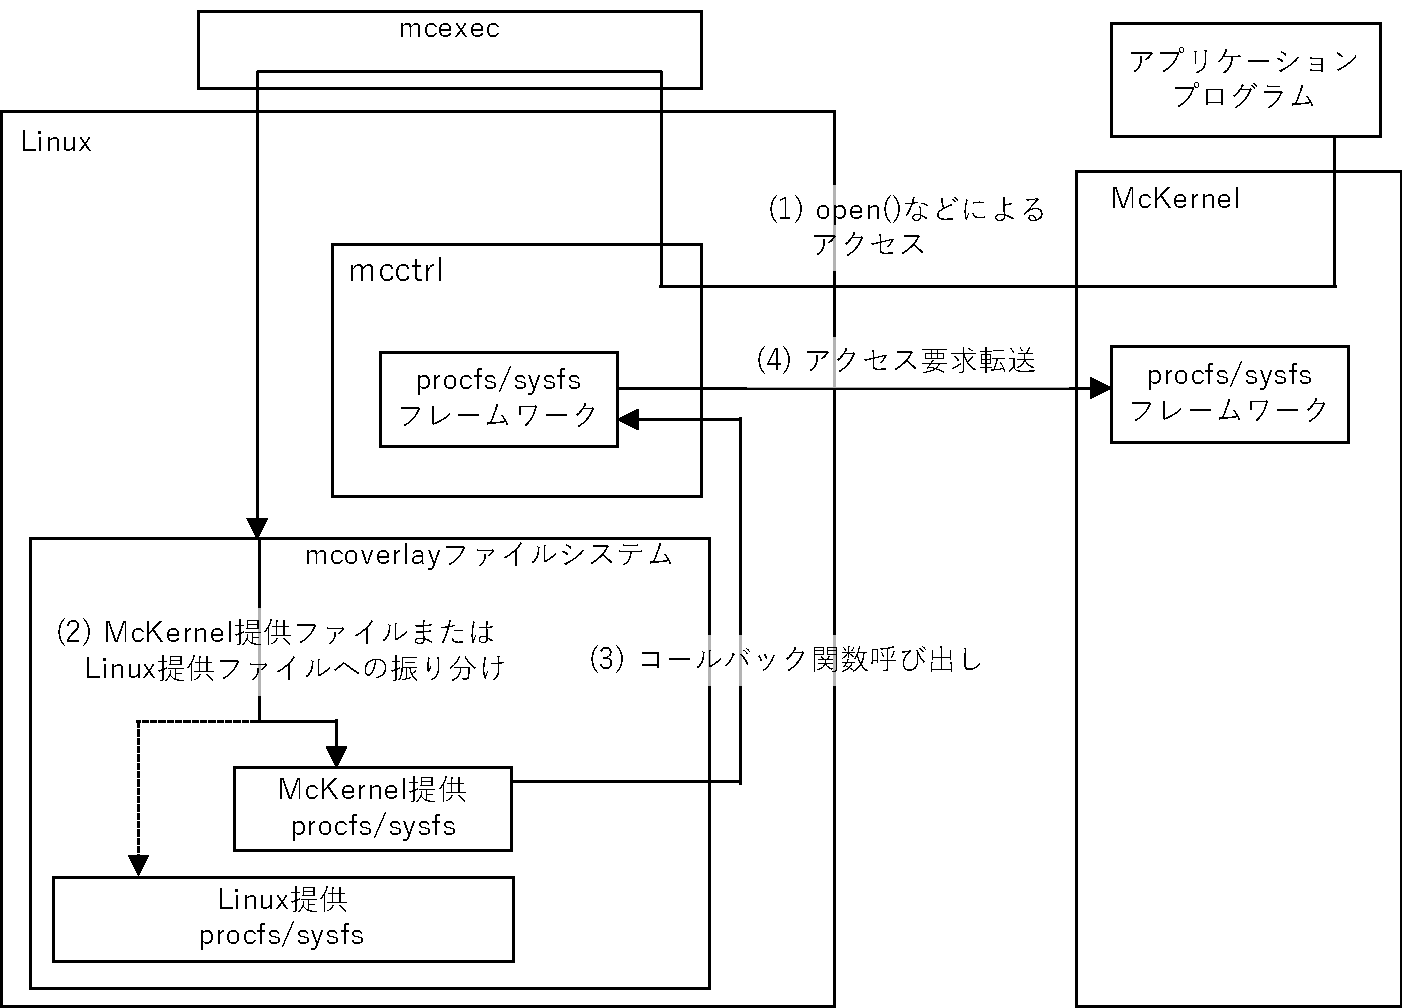
\includegraphics[width=12cm]{figs/procfs_access.pdf}
\vspace{-0em}\caption{\texttt{procfs/sysfs}のアクセス要求転送}
\label{fig:spec-os-mck-procfs-access}
\vspace{-0em}
\end{figure}
%
\begin{enumerate}
\item アプリは\texttt{open()}などのシステムコールを用いてprocfs/sysfsのファイルへのアクセスを試みる。このシステムコールの処理はLinux側に転送される。(図の(1))
\item \texttt{mcexec}がシステムコールを代理実行する。\texttt{mcoverlayfs}が優先度に基づいてMcKernelが提供するファイルまたはLinuxが提供するファイルへのアクセス振り分けを行う。この場合は前者に振り分けられたとする。(図の(2))
\item McKernelが提供するファイルに登録されたコールバック関数が呼び出される。(図の(3))
\item Linux側\texttt{procfs/sysfs}フレームワークがアクセス要求をMcKernel側フレームワークに転送する。McKernel側フレームワークはアクセスに応じた処理を行う。例えば、ファイルの内容を返却する。(図の(4))
\end{enumerate}
\FloatBarrier

\section{\MODAUGS{ファイルシステム重ね合わせ}}\label{sec:mcoverlayfs}
McKernelはカーネルモジュール\texttt{mcoverlayfs}によって2つのファイルシステムを優先度付きで重ね合わせることができる。
本機能は\texttt{procfs/sysfs}機能のために用いられる。

\texttt{mcoverlayfs}は\texttt{overlayfs}に以下の機能を追加することで実装されている。
\begin{enumerate}
\item copyup処理無効化\\
\texttt{mcoverlayfs}はlowerdirとupperdirに重ね合わせたいファイルシステムを指定する。
McKernelでは、lowerdirに、McKernelがその内容を提供する\texttt{procfs/sysfs}とLinuxのそれとを指定して用いる。
overlayfsでは、ライト対象のファイルがlowerdir上のファイルの場合、copyup処理を行いupperdirに対象ファイルを作成し、そのファイルをオープンすることで、ライト処理を可能とする。
このようにすると、アクセス要求は\texttt{procfs/sysfs}に届かない。
そのため、copyup処理を無効化し、直接対象ファイルにライト処理する機能を追加する。
本機能はオプションにnocopyupwを指定することで有効となる。

nocopyupwオプションの有無によるライト処理の違いを図 \ref{figure:chap05_fig001}に示す。
\begin{figure}[ht]
  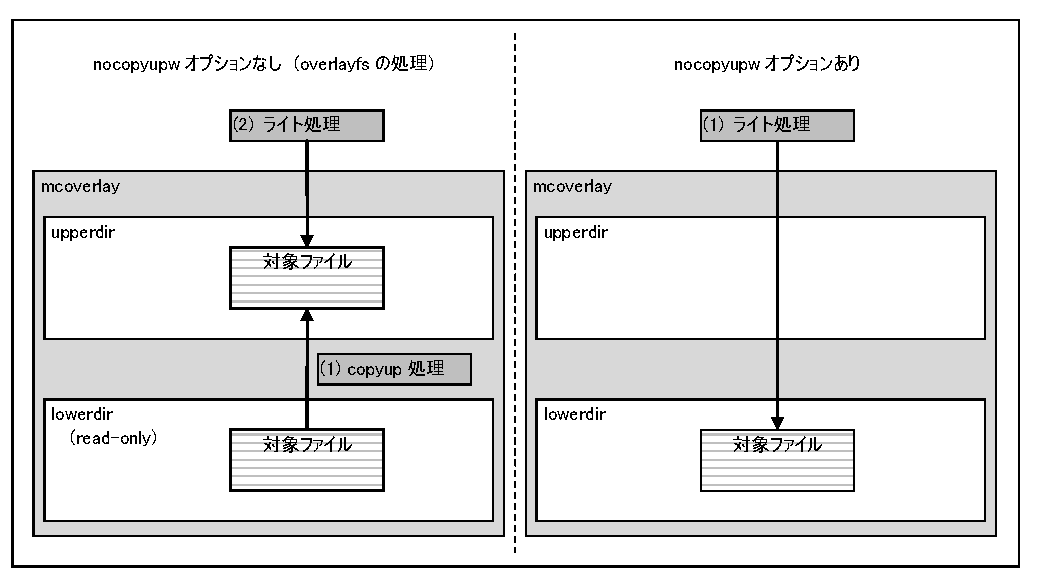
\includegraphics[scale=0.85]{figs/chap05_fig001.pdf}
  \caption{nocopyupwオプションの有無によるライト処理の違い}
  \label{figure:chap05_fig001}
\end{figure}

\begin{itemize}
  \item nocopyupwオプションなしで、ライト対象のファイルがlowerdir上のファイルの場合、copyup処理を行いupperdirに対象ファイルを作成し、そのファイルをオープンすることで、ライト処理を可能とする。
  \item nocopyupwオプションありの場合、ライト対象のファイルがlowerdir上のファイルの場合でも、copyup処理せず、そのファイルをオープンすることで、ライト処理を可能とする。
\end{itemize}

\item procfs/sysfsサポート\\
\texttt{mcoverlayfs}では\texttt{overlayfs}に対してprocfs/sysfsのディレクトリのマウント機能を追加している。
本機能はオプションにnofscheckを指定することで有効となる。
\end{enumerate}

\comment{
また、nocopyupwオプションありの場合、copyup処理が発生してしまうstruct inode\_operationsの以下の操作については無効とする。
\begin{enumerate}
  \item setattr
  \item setxattr
  \item getxattr
\end{enumerate}

\subsection{vfs\_open()の処理変更に伴う対応}
仮想ファイルシステム(VFS)は、Linux-4.0からLinux-4.6になって、struct inode\_operationsのdentry\_open()が削除されて、struct dentry\_operationsのd\_select\_inode()が追加された。そして、VFSのvfs\_open()では、dentry\_open()が呼ばれずに、d\_select\_inode()が呼び出されるようになった。

\begin{verbatim}
// 削除されたstruct inode_operationsのdentry_open()
struct inode_operations {
    int (*dentry_open)(struct inode *, struct file *, const struct cred *);
}

// 追加されたstruct dentry_operationsのd_select_inode()
struct dentry_operations {
    struct inode *(*d_select_inode)(struct dentry *, unsigned);
}
\end{verbatim}

この変更で、VFSで対象ファイルのopen()時に指定するstruct inodeにはオープンする対象ファイル、struct fileにはoverlayfsのファイルが指定されて処理するようになった。しかし、sysfsの場合、struct file\_operationsのint (*open)(struct inode *, struct file *)で、struct fileが示すf\_pathのstruct dentryのvoid *d\_fsdataを参照して処理するためエラーとなることが分かった。

\begin{verbatim}
// struct file_operationsのopen()
struct file_operations {
    int (*open)(struct inode *, struct file *);
}
\end{verbatim}

sysfsの場合、fileとinodeを参照して処理する際にエラーとなる。(fileはoverlayfsのファイル、inodeはsysfsのファイルを示しているため。)

他のファイルシステムの場合、inodeのみ参照してopen処理しているため問題ない。\\

この対策として、nofscheckオプションありの場合、d\_select\_inode()で、対象ファイルがsysfsの場合のみ、struct fileが示すf\_pathのstruct dentryのvoid *d\_fsdataを\texttt{mcoverlayfs}のd\_fsdataからsysfsのd\_fsdataに置き換えることでopen()時にエラーが発生しないように対応する。
置き換える際には、\texttt{mcoverlayfs}のd\_fsdataをstruct ovl\_fsのd\_fsdata\_listに登録して、\texttt{mcoverlayfs}の処理で使用できるようにする。

\texttt{mcoverlayfs}の処理で\texttt{mcoverlayfs}のd\_fsdataを使用する際には、ovl\_reset\_ovl\_entry()を呼び出すことでstruct ovl\_fsのd\_fsdata\_listに登録した\texttt{mcoverlayfs}のd\_fsdataを取得する。

vfs\_openのシーケンス(linux-4.0及び、linux-3.10.0-327の場合)を図 \ref{figure:chap05_fig002}に示す。
\begin{figure}[ht]
  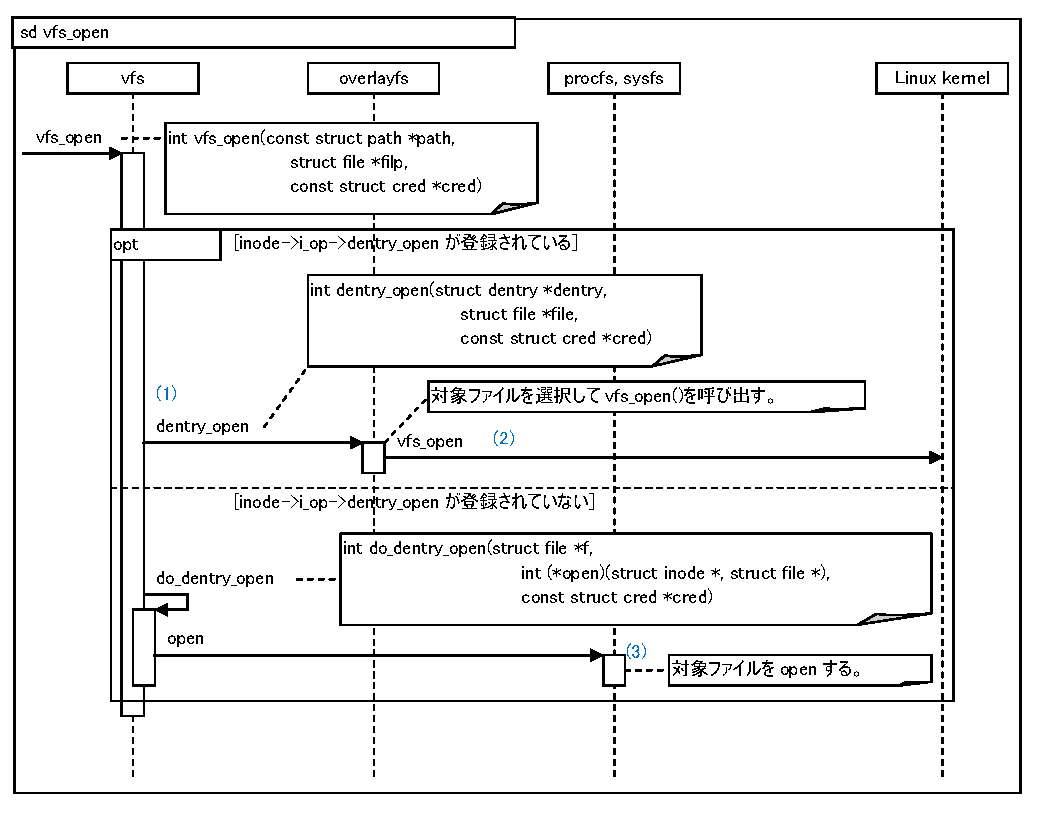
\includegraphics[scale=0.85]{figs/chap05_fig002.pdf}
  \caption{vfs\_openのシーケンス(linux-4.0及び、linux-3.10.0-327の場合)}
  \label{figure:chap05_fig002}
\end{figure}

\begin{enumerate}
  \item openするファイルがoverlayfsの場合、overlayfsのdentry\_open()が呼び出される。
  \item overlayfsのdentry\_open()で、処理の対象になるファイルを選択して、vfs\_open()を呼び出す。
  \item 対象ファイルのファイルシステムのopen()が処理される。
\end{enumerate}

vfs\_openのシーケンス(linux-4.6の場合)を図 \ref{figure:chap05_fig003}に示す。
\begin{figure}[ht]
  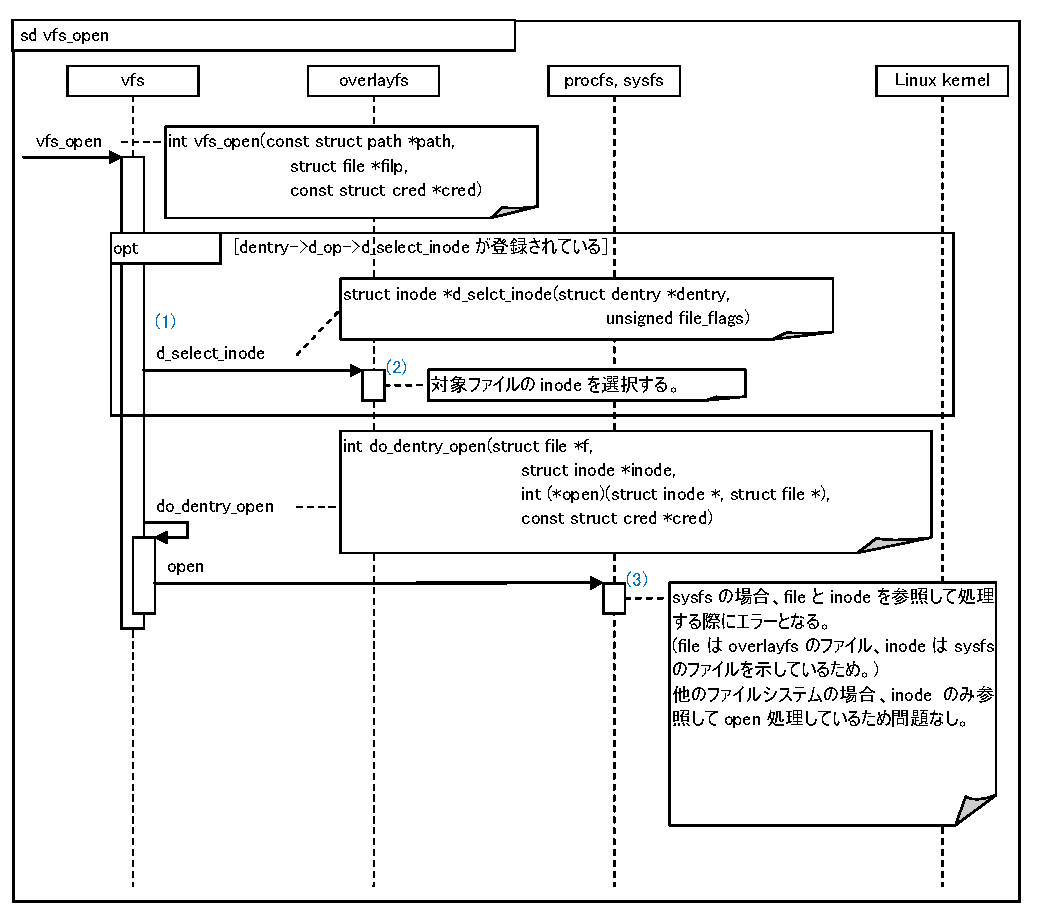
\includegraphics[scale=0.85]{figs/chap05_fig003.pdf}
  \caption{vfs\_openのシーケンス(linux-4.6の場合)}
  \label{figure:chap05_fig003}
\end{figure}

\begin{enumerate}
  \item openするファイルがoverlayfsの場合、overlayfsのd\_select\_inode()が呼び出される。
  \item overlayfsのd\_select\_inode()で、処理の対象になるファイルを選択して、そのファイルのinodeを戻す。
  \item 対象ファイルのファイルシステムのopen()が処理される。
\end{enumerate}
}

\texttt{mcoverlayfs}のマウントオプションを表\ref{table:mcoverlayfs_options} に示す。
\texttt{nocopyupw, nofscheck}が\texttt{overlayfs}に対して追加されたオプションである。
\begin{table}[!h]
  \caption{\texttt{mcoverlayfs}のマウントオプション}
  \label{table:mcoverlayfs_options}
  \begin{tabular}{|p{0.30\linewidth}|p{0.65\linewidth}|} \hline
     オプション & 説明 \\ \hline
     \texttt{lowerdir=<dirs>}      & lowerdirを指定する。                  \\
                                   & ':'で区切り複数指定可能(最大500)      \\ \hline
     \texttt{upperdir=<dir>}       & upperdirを指定する。                  \\ \hline
     \texttt{workdir=<dir>}        & workdirを指定する。                   \\
                          & workdirは、upperdirと同じマウント下のディレクトリでなければならない。  \\ \hline
     \texttt{default\_permissions} & デフォルトパーミッションを設定する。  \\ \hline
     \texttt{nocopyupw}            & 書き込み時にupperdirにファイルを作成し、それに対して書き込みを行う処理(copyup処理)を無効にする。\texttt{procfs/sysfs}をlowerdirに指定する際は本オプションを指定する必要がある。      \\ \hline
     \texttt{nofscheck}            & \texttt{procfs/sysfs}をlowerdirに指定可能にする。  \\ \hline
  \end{tabular}
\end{table}
\FloatBarrier

\subsection{詳細}

\texttt{overlayfs}のデータ構造に対する修正は以下の通り。
\begin{enumerate}
\item \texttt{ovl\_opt\_bit}\\
マウントオプションを追加するために、以下のenum及び、マクロを追加する。
\footnotesize
\begin{verbatim}
enum ovl_opt_bit {
        __OVL_OPT_DEFAULT       = 0,
        __OVL_OPT_NOCOPYUPW     = (1 << 0),
        __OVL_OPT_NOFSCHECK     = (1 << 1),
};

#define OVL_OPT_NOCOPYUPW(opt)  ((opt) & __OVL_OPT_NOCOPYUPW)
#define OVL_OPT_NOFSCHECK(opt)  ((opt) & __OVL_OPT_NOFSCHECK)
\end{verbatim}
\normalsize

\item \texttt{ovl\_d\_fsdata}\\
d\_fsdataを格納するために、以下の構造体を追加する。
\footnotesize
\begin{verbatim}
struct ovl_d_fsdata {
        struct list_head list;
        struct dentry *d;
        struct ovl_entry *oe;
};
\end{verbatim}
\normalsize

\item \texttt{ovl\_config}\\
マウントオプションを追加するために、optを追加する。
\footnotesize
\begin{verbatim}
struct ovl_config {
        char *lowerdir;
        char *upperdir;
        char *workdir;
        bool default_permissions;
        unsigned opt;              <-- 追加
};
\end{verbatim}
\normalsize

\item \texttt{ovl\_fs}\\
d\_fsdataを格納するために、d\_fsdata\_listを追加する。
\footnotesize
\begin{verbatim}
struct ovl_fs {
        struct vfsmount *upper_mnt;
        unsigned numlower;
        struct vfsmount **lower_mnt;
        struct dentry *workdir;
        long lower_namelen;
        /* pathnames of lower and upper dirs, for show_options */
        struct ovl_config config;
        struct list_head d_fsdata_list;  <-- 追加
};
\end{verbatim}
\normalsize

\item \texttt{ovl\_tokens}\\
マウントオプションを追加するために、OPT\_NOCOPYUPW及び、OPT\_NOFSCHECKを追加する。
\footnotesize
\begin{verbatim}
enum {
        OPT_LOWERDIR,
        OPT_UPPERDIR,
        OPT_WORKDIR,
        OPT_DEFAULT_PERMISSIONS,
        OPT_NOCOPYUPW,            <-- 追加
        OPT_NOFSCHECK,            <-- 追加
        OPT_ERR,
};

static const match_table_t ovl_tokens = {
        {OPT_LOWERDIR,                  "lowerdir=%s"},
        {OPT_UPPERDIR,                  "upperdir=%s"},
        {OPT_WORKDIR,                   "workdir=%s"},
        {OPT_DEFAULT_PERMISSIONS,       "default_permissions"},
        {OPT_NOCOPYUPW,                 "nocopyupw"},            <-- 追加
        {OPT_NOFSCHECK,                 "nofscheck"},            <-- 追加
        {OPT_ERR,                       NULL}
};
\end{verbatim}
\normalsize

\item \texttt{ovl\_fs\_type}\\
nameの値を"mcoverlay"に変更する。
\footnotesize
\begin{verbatim}
static struct file_system_type ovl_fs_type = {
        .owner          = THIS_MODULE,
        .name           = "mcoverlay",      <-- 変更
        .mount          = ovl_mount,
        .kill_sb        = kill_anon_super,
};
MODULE_ALIAS_FS("mcoverlay");               <-- 変更
\end{verbatim}
\normalsize
\end{enumerate}

\comment{
\texttt{mcoverlayfs}のソースファイルを表 \ref{table:chap05_src_files} に示す。

区分は、Linux-4.6.7のoverlayfsのソースコードに変更を加えるかを示す。

('—'は、変更しないことを示す。)

\begin{table}[ht]
  \caption{\texttt{mcoverlayfs}のソースファイル}
  \label{table:chap05_src_files}
  \begin{tabular}{|l|p{8cm}|p{2cm}|l|} \hline
    No. & ファイル & 区分 & 備考 \\ \hline
    1  & overlayfs.h & 変更 & \\ \hline
    2  & copy\_up.c  & 変更 & \\ \hline
    3  & dir.c       & 変更 & \\ \hline
    4  & inode.c     & 変更 & \\ \hline
    5  & readdir.c   & —   & \\ \hline
    6  & super.c     & 変更 & \\ \hline
  \end{tabular}
\end{table}
}

\texttt{overlayfs}に対する関数の修正を表\ref{tab:overlayfs1}、表\ref{tab:overlayfs2}に示す。
\begin{table}[!h]
\caption{\texttt{overlayfs}の関数に対する修正(1)}\label{tab:overlayfs1}
\footnotesize
\begin{tabular}{|p{0.30\linewidth}|p{0.65\linewidth}|} \hline
\multicolumn{1}{|c}{\textbf{関数}}&\multicolumn{1}{|c|}{\textbf{修正内容}}\\ \hline \hline
\texttt{ovl\_copy\_xattr()}&\texttt{OVL\_OPT\_NOFSCHECK(opt)}が有効の場合、vfs\_getxattr()のエラーを無視する。\\ \hline
\texttt{ovl\_copy\_up\_locked()}&\texttt{ovl\_copy\_xattr()}呼び出し時に\texttt{ovl\_get\_config\_opt()}で取得したopt値を渡す。\\ \hline
\texttt{ovl\_clear\_empty()}&\texttt{ovl\_copy\_xattr()}呼び出し時に\texttt{ovl\_get\_config\_opt()}で取得したopt値を渡す。\\ \hline
\texttt{ovl\_setattr()}&\begin{tabular}[t]{@{}l@{}}\texttt{ovl\_get\_config\_opt()}でopt値を取得する。\\ \texttt{OVL\_OPT\_NOCOPYUPW(opt)}の場合、処理しない。\end{tabular}\\ \hline
\texttt{ovl\_permission()}& \texttt{ovl\_reset\_ovl\_entry()}を呼び出してから処理する。\\ \hline
\texttt{ovl\_setxattr()}&\begin{tabular}[t]{@{}l@{}}\texttt{ovl\_get\_config\_opt()}でopt値を取得する。\\\texttt{OVL\_OPT\_NOCOPYUPW(opt)}の場合、処理しない。\end{tabular}\\ \hline
\texttt{ovl\_removexattr()}&\begin{tabular}[t]{@{}l@{}}\texttt{ovl\_get\_config\_opt()}でopt値を取得する。\\\texttt{OVL\_OPT\_NOCOPYUPW(opt)}の場合、処理しない。\end{tabular}\\ \hline
\texttt{ovl\_d\_select\_inode()}&
\begin{tabular}[t]{@{}l@{}}
   1. \texttt{ovl\_get\_config\_opt()}でopt値を取得する。\\
   2. \texttt{OVL\_OPT\_NOCOPYUPW(opt)}の場合、\texttt{ovl\_open\_need\_copy\_up()}を\\
   {\quad}呼び出さない。\\
   3. \texttt{OVL\_OPT\_NOFSCHECK(opt)}で対象ファイルがsysfsの場合、\\
   {\quad}\texttt{ovl\_find\_d\_fsdata()}を呼び出してdentryが登録されているか確認\\
   {\quad}する。登録されていない場合には\texttt{ovl\_add\_d\_fsdata()}を呼び出して\\
   {\quad}登録し、\texttt{dentry->d\_fsdata}に\texttt{realpath.dentry->d\_fsdata}\\
   {\quad}の値を設定する。\\
\end{tabular}\\ \hline
\texttt{ovl\_get\_config\_opt()}&\texttt{opt}値を返す。\\ \hline
\texttt{ovl\_reset\_ovl\_entry()}&
\begin{tabular}[t]{@{}l@{}}
1.  \texttt{ovl\_get\_config\_opt()}でopt値を取得する。\\
2.  \texttt{OVL\_OPT\_NOFSCHECK(opt)}の場合、\texttt{ovl\_find\_d\_fsdata()}を呼び出し\\
{\quad}て、dentryが登録されている場合には取得した\texttt{d\_fsdata}を\texttt{oe}に\\
{\quad}設定する。\\
\end{tabular}\\ \hline
\texttt{ovl\_find\_d\_fsdata()}&\texttt{dentry->d\_sb->s\_fs\_info}の\texttt{d\_fsdata\_list}に登録されている\texttt{d\_fsdata}を検索して、\texttt{dentry}が登録されていた場合、\texttt{dentry}の\texttt{ovl\_entry}を戻す。\\ \hline
\texttt{ovl\_add\_d\_fsdata()}&
\begin{tabular}[t]{@{}l@{}}
1. \texttt{struct ovl\_d\_fsdata}のメモリ領域を確保して、\texttt{dentry}の登録デー\\
{\quad}タを設定する。\\
2. \texttt{dentry->d\_sb->s\_fs\_info}の\texttt{d\_fsdata\_list}に登録する。
\end{tabular}\\ \hline
\texttt{ovl\_clear\_d\_fsdata()}&\texttt{d\_fsdata\_list}に登録されている全ての\texttt{d\_fsdata}を削除して、\texttt{struct ovl\_d\_fsdata}のメモリ領域を解放する。\\ \hline
\texttt{ovl\_path\_type()}&\multirow{16}{\linewidth}{\texttt{ovl\_reset\_ovl\_entry()}を呼び出してから処理する。}\\ \cline{1-1}
\texttt{ovl\_path\_upper()}& \\ \cline{1-1}
\texttt{ovl\_dentry\_upper()}& \\ \cline{1-1}
\texttt{ovl\_dentry\_lower()}& \\ \cline{1-1}
\texttt{ovl\_dentry\_real()}&\\ \cline{1-1}
\texttt{ovl\_dir\_cache()}&\\ \cline{1-1}
\texttt{ovl\_set\_dir\_cache()}&\\ \cline{1-1}
\texttt{ovl\_path\_lower()}&\\ \cline{1-1}
\texttt{ovl\_dentry\_is\_opaque()}&\\ \cline{1-1}
\texttt{ovl\_dentry\_set\_opaque()}&\\ \cline{1-1}
\texttt{ovl\_dentry\_update()}&\\ \cline{1-1}
\texttt{ovl\_dentry\_version\_inc()}& \\ \cline{1-1}
\texttt{ovl\_dentry\_version\_get()}&\\ \cline{1-1}
\texttt{ovl\_dentry\_release()}&  \\ \cline{1-1}
\texttt{ovl\_dentry\_revalidate()}&  \\ \cline{1-1}
\texttt{ovl\_dentry\_weak\_revalidate()}&  \\ \cline{1-2}

\end{tabular}
\vspace{-0em}
\end{table}
\FloatBarrier

\begin{table}[!h]
\caption{\texttt{overlayfs}の関数に対する修正(2)}\label{tab:overlayfs2}
\footnotesize
\begin{tabular}{|p{0.30\linewidth}|p{0.65\linewidth}|} \hline
\multicolumn{1}{|c}{\textbf{関数}}&\multicolumn{1}{|c|}{\textbf{修正内容}}\\ \hline \hline
\texttt{ovl\_lookup\_real()}&\texttt{OVL\_OPT\_NOFSCHECK(opt)}の場合、\texttt{ovl\_dentry\_weird()}を呼び出さない。\\ \hline

\texttt{ovl\_path\_next()}&\texttt{ovl\_reset\_ovl\_entry()}を呼び出してから処理する。\\ \hline
\texttt{ovl\_lookup()}&
\begin{tabular}[t]{@{}l@{}}
1. \texttt{ovl\_get\_config\_opt()}でopt値を取得する。\\
2. \texttt{ovl\_reset\_ovl\_entry()}を呼び出してから処理する。\\
3. \texttt{ovl\_lookup\_real()}を呼び出す際、opt値を渡す。\\
\end{tabular} \\ \hline

\texttt{ovl\_put\_super()}&\texttt{ovl\_clear\_d\_fsdata()}を呼び出してから処理する。\\ \hline
\texttt{ovl\_statfs()}&\texttt{struct kstatfs}の\texttt{f\_type}に\texttt{MCOVERLAYFS\_SUPER\_MAGIC}を設定する。\\ \hline
\texttt{ovl\_show\_options()}&\texttt{nocopyupw, nofscheck}オプションの説明を追加する。\\ \hline
\texttt{ovl\_parse\_opt()}&\texttt{nocopyupw, nofscheck}オプションの設定を追加する。\\ \hline
\texttt{ovl\_mount\_dir\_noesc()}&\texttt{OVL\_OPT\_NOFSCHECK(opt)}の場合、\texttt{ovl\_dentry\_weird()}を呼び出さない。\\ \hline
\texttt{ovl\_mount\_dir()}&\texttt{ovl\_mount\_dir\_noesc()}を呼び出す際、\texttt{opt}を渡す。\\ \hline
\texttt{ovl\_lower\_dir()}&\texttt{ovl\_mount\_dir\_noesc()}を呼び出す際、\texttt{opt}を渡す。\\ \hline
\texttt{ovl\_fill\_super()}&
\begin{tabular}[t]{@{}l@{}}
  1. \texttt{struct ovl\_fs}の\texttt{d\_fsdata\_list}を初期化する。\\
  2. \texttt{ovl\_mount\_dir()}を呼び出す際、\texttt{opt}を渡す。\\
  3. \texttt{ovl\_lower\_dir()}を呼び出す際、\texttt{opt}を渡す。\\
  4. \texttt{OVL\_OPT\_NOCOPYUPW(opt)}の場合、以下の設定を行わない。\\
\begin{tabular}[t]{@{}l@{}}
{\quad}\textbullet~~\texttt{mnt->mnt\_flags |= MNT\_READONLY};\\
{\quad}\textbullet~~\texttt{sb->s\_flags |= MS\_RDONLY};\\
\end{tabular}
\end{tabular} \\ \hline

\end{tabular}
\vspace{-0em}
\end{table}
\FloatBarrier

\subsection{\MODAUGS{実装の制限}}
McKernelが生成する\texttt{/proc/{\lbrack}pid{\rbrack}/}下のファイルをopenして、closeせずにopenした状態でexecして、execしたプロセスで同一ファイルをopenするとエラー(\texttt{ENOENT})となる。
原因は、\texttt{exec()}時には、新たなプロセスの情報を返せるようにするため\texttt{/proc/{\lbrack}pid{\rbrack}/}下のファイルを作成し直すが、overlayfsは\texttt{lower}に指定されるディレクトリ下のファイルのinode番号が変わった場合、エラーを返すためである。

\subsection{\ADDAUGS{開発時の留意事項}}
Linux-4.0からLinux-4.6への移行に際する仮想ファイルシステムの以下の仕様変更に追従する必要があった。
\begin{enumerate}
\item \texttt{struct inode\_operationsのdentry\_open()}が削除されて、\texttt{struct dentry\_operations}の\texttt{d\_select\_inode()}が追加された。
\item VFSの\texttt{vfs\_open()}では、\texttt{dentry\_open()}が呼ばれずに、\texttt{d\_select\_inode()}が呼び出されるようになった。
\end{enumerate}

また、以下のバージョンのLinuxカーネルでのみ動作する。
\begin{itemize}
\item 3.10.0-327から3.10.0-693(RHEL-7.2から7.4)
\item 4.0.0から4.1.0
\item 4.6.0から4.7.0
\end{itemize}



\comment{
\texttt{/proc/{\lbrack}pid{\rbrack}/}下のファイルは、
\texttt{exec()}時に\texttt{mcexec}が\texttt{mcctrl}に作成を依頼し、
\texttt{mcctrl}が\texttt{mcexec\_open\_exec()}で\texttt{add\_procfs\_entry()}を用いて作成する。
%\texttt{mcexec}が\texttt{/dev/mcos}に\texttt{ioctl()}の\texttt{MCEXEC\_UP\_OPEN\_EXEC}で、
}

\section{\MODAUGS{デバイスドライバ}}
McKernelでは、Linuxで動作するドライバをそのまま利用可能であるが、システムコール移譲のオーバーヘッドを削減するために、McKernel内部で実装することもできる。

以下、それぞれの方法を説明する。

\subsection{Linuxドライバの利用}
Linuxドライバ経由でメモリマップされたデバイスのレジスタをMcKernelプロセスからアクセス可能にすることで、Linuxドライバをそのまま利用できるようにする。

動作を図\ref{fig:device_map}を用いて説明する。
%
\begin{figure}[htb]
\centering
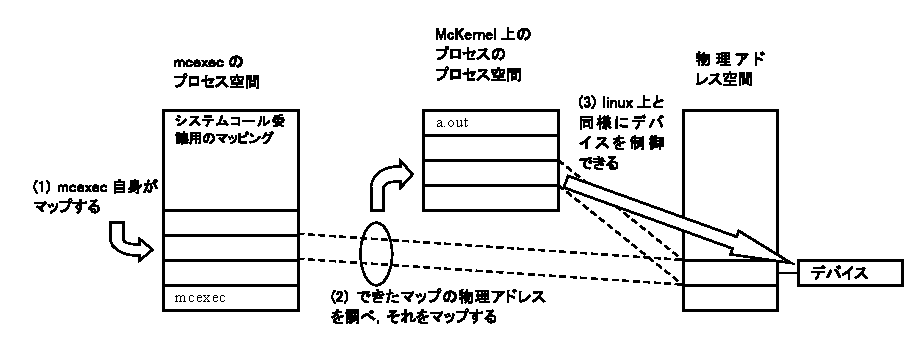
\includegraphics[width=12cm]{figs/device_map.pdf}
\vspace{-0em}\caption{Linuxドライバ利用の動作}
\label{fig:device_map}
\vspace{-0em}
\end{figure}
%
\begin{enumerate}
\item システムコール移譲の仕組みを用いてデバイスファイルの\texttt{open(), ioctl()}を行う。
\item レジスタのマップについてはシステムコール移譲の仕組みを用いて、\texttt{mcexec}空間へのマップと、McKernelの仮想メモリ領域構造体への特別なマップであることの記録を行う。(図の(1))
\item McKernelでのページフォールトの際にLinuxに物理ページを問い合わせ、同じ物理ページを参照するマップをMcKernel上のプロセス空間に作成する。(図の(2))
\end{enumerate}
\FloatBarrier

\comment{
図\ref{fig:device_map_dt}と表\ref{tab:device_map_dt}に関連データ構造を示す。
これらのうち、devobjを新規に作成し、fileobjと、pager、pagerインタフェースを改造した。
\begin{figure}[htb]
\centering
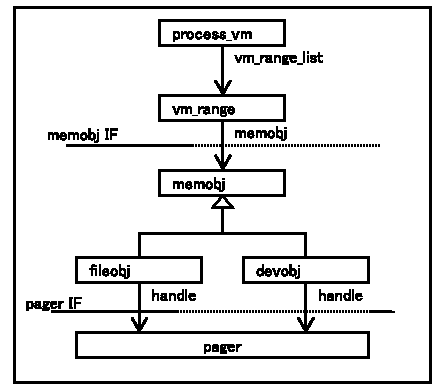
\includegraphics[width=10cm]{figs/device_map_dt.pdf}
\vspace{-0em}\caption{McKernelのメモリ管理のデータ構造}
\label{fig:device_map_dt}
\vspace{-0em}
\end{figure}
\FloatBarrier

\begin{table}[!htb]
\centering
\footnotesize
\caption{メモリ管理用構造体一覧}\vspace{0.0em}
\label{tab:device_map_dt}
\begin{tabular}{|p{0.15\linewidth}|p{0.70\linewidth}|} \hline
\multicolumn{1}{|c}{\textbf{構造体名}}&\multicolumn{1}{|c|}{\textbf{説明}}\\ \hline \hline
\texttt{process\_vm}&プロセス空間を実現する\\ \hline
\texttt{page\_table}&cpuのページテーブルを実現する\\ \hline
\texttt{vm\_range}&仮想連続かつ同じ属性を持つ、仮想ページの集合を管理する。\\ \hline
\texttt{memobj}&物理ページの集合を管理する\\ \hline
\texttt{devobj}&デバイスファイルをバックエンドとする物理ページの集合を管理する\\ \hline
\texttt{fileobj}&レギュラファイルをバックエンドとする物理ページの集合を管理する\\ \hline
\texttt{pager}&バックエンドとなっているファイルの操作を実現する。\\ \hline
\end{tabular}
\vspace{-0em}
\end{table}
\FloatBarrier

\texttt{memobj}は、\texttt{memobj}インタフェースを提供するための抽象的な構造体で、devobjやfileobjなどの具体的な構造体の一部として同時に作成される。

\texttt{memobj}インタフェースを表\ref{tab:memobjif}に示す。
\begin{table}[!htb]
\centering
\footnotesize
\caption{\texttt{memobj}インタフェース一覧}\vspace{0.0em}
\label{tab:memobjif}
\begin{tabular}{|p{0.10\linewidth}|p{0.75\linewidth}|} \hline
\multicolumn{1}{|c}{\textbf{名称}}&\multicolumn{1}{|c|}{\textbf{説明}}\\ \hline \hline
\texttt{(create)}&\texttt{memobj}を作成する。実際には、各具象\texttt{memobj}固有の作成関数で作成する。\\ \hline
\texttt{ref}&\texttt{memobj}の参照数を増やす\\ \hline
\texttt{release}&\texttt{memobj}の参照を減らす\\ \hline
\texttt{get\_page}&物理ページのアドレスを取得する\\ \hline
\texttt{copy\_page}&未使用\\ \hline
\texttt{flush\_page}&物理ページの内容をバックエンドに直ちに書き戻す\\ \hline
\end{tabular}
\vspace{-0em}
\end{table}
\FloatBarrier

pagerインタフェースを表\ref{tab:pagerif}に示す。
\begin{table}[!htb]
\centering
\footnotesize
\caption{pagerインタフェース一覧}\vspace{0.0em}
\label{tab:pagerif}
\begin{tabular}{|p{0.20\linewidth}|p{0.65\linewidth}|} \hline
\multicolumn{1}{|c}{\textbf{名称}}&\multicolumn{1}{|c|}{\textbf{説明}}\\ \hline \hline
\texttt{PAGER\_REQ\_CREATE}&レギュラファイルをバックエンドとするpagerを作成する。既にpagerが存在する場合は、共用する。\\ \hline
\texttt{PAGER\_REQ\_READ}&ページイン。McKernel上の指定された物理ページにファイルの内容を読み出す。\\ \hline
\texttt{PAGER\_REQ\_WRITE}&ページアウト。McKernel上の指定された物理ページからファイルに書き込む。\\ \hline
\texttt{PAGER\_REQ\_RELEASE}&\texttt{PAGER\_REQ\_CREATE}で作成されたpagerの参照を解放する。pagerを参照するfileobjが無くなった時、pagerは解放される。\\ \hline
\texttt{PAGER\_REQ\_MAP}&デバイスファイルをバックエンドとするpagerを作成する。同じファイルのpagerが存在しても新たに作成することに注意。\\ \hline
\texttt{PAGER\_REQ\_PFN}&指定されたオフセットに対応する物理ページの物理アドレスを取得する\\ \hline
\texttt{PAGER\_REQ\_UNMAP}&\texttt{PAGER\_REQ\_MAP}で作成したpagerの解放。\\ \hline
\end{tabular}
\vspace{-0em}
\end{table}
\FloatBarrier
}

\comment{
\subsubsection{動作}
レギュラファイルとデバイスファイルとでのマッピング処理の違いを、使用する\texttt{memobj}の違いにまとめることで、それ以外のプロセス空間操作やPTE操作を共用する。
レギュラファイルの場合fileobj構造体を使用し、デバイスファイルの場合devobjを使用する。

\subsubsubsection{mmap時}
McKernelでは、fdが示すファイルがレギュラファイルなのかデバイスファイルなのか判断できない。そこで、まずfileobj構造体、次にdevobj構造体の作成を試みる。これらの構造体の作成処理の延長でホストへpager作成要求が発行されるので、そのタイミングでfdが示すファイルの種別を判定できる。作成する構造体に不適切なファイル種別の場合、構造体の作成を失敗させて次の構造体の作成に進ませる。
fileobjの作成を先に試みるのは、デバイスファイルに比べてレギュラファイルがマップされる可能性が高いと考えるからである。また、無駄にdevobjの作成を試みることを避けるために、fdがデバイスファイルであることを理由にfileobj作成処理を中断するとき、特別なエラーコード (ESRCH) を返させる。このエラーコードでfileobj構造体作成に失敗したときのみ、devobj構造体の作成を試みる。

devobjの作成処理手順は以下の通り。
\begin{enumerate}
\item McKernelは、\texttt{PAGER\_REQ\_MAP}要求をホストに送り、ホスト側のpagerの作成を要求する。
\item \texttt{PAGER\_REQ\_MAP}を受けたホストは、\texttt{do\_mmap\_pgoff()} を使用して、指定されたデバイスファイルをマップする。\texttt{do\_mmap\_pgoff()}の呼び出し方は後で述べる。
\item ホストは、でき上ったマッピングを管理するpager構造体を作成し、\texttt{PAGER\_REQ\_MAP}の応答をMcKernelに返す。
\item 応答を受け取ったMcKernelは、devobj構造体にpagerの情報を格納し、作成したdevobjをmmapに返す。
\end{enumerate}

デバイスファイルのマッピングの場合、pager構造体はマップのつど作成する。たとえ同じプロセスが同じデバイスファイルを複数回マップしたとしても、pager構造体およびdevobj構造体は共用しない。これは、同じデバイスファイルであっても、マップするプロセス・タイミングによって異なる物理ページがマップされることが予想されるからである。
なお、レギュラファイルのマッピングの場合、pager構造体およびfileobj構造体はlinuxのinodeと一対一対応で作成し、別プロセスであっても同じファイルのマップであればこれらを共用する。
\texttt{do\_mmap\_pgoff()}の引数の作成方法を表\ref{tab:do_mmap_pgoff_options}に示す。

\begin{table}[!htb]
\centering
\footnotesize
\caption{\texttt{do\_mmap\_pgoff()} の引数の作り方}\vspace{0.0em}
\label{tab:do_mmap_pgoff_options}
\begin{tabular}{|p{0.10\linewidth}|p{0.75\linewidth}|} \hline
\multicolumn{1}{|c}{\textbf{名称}}&\multicolumn{1}{|c|}{\textbf{説明}}\\ \hline \hline
\texttt{file}&mmapの引数\texttt{fd}が示すfile構造体\\ \hline
\texttt{addr}&NULL固定。mcexec空間内の空いているところにマップさせるため。\\ \hline
\texttt{len}&mmapの引数\texttt{len}\\ \hline
\texttt{prot}&\texttt{PROT\_READ}、\texttt{PROT\_WRITE}、\texttt{PROT\_EXEC}のうち、mmapの引数fdに許されるものすべて\\ \hline
\texttt{flags}&\texttt{MAP\_SHARED}固定\\ \hline
\texttt{pgoff}&mmapの引数\texttt{off}を\texttt{PAGE\_SIZE}で割ったもの\\ \hline
\end{tabular}
\vspace{-0em}
\end{table}
\FloatBarrier

\subsubsubsection{アクセス時}
デバイスマッピングも、ファイルマッピングと同様に、ユーザプロセスが仮想ページに最初にアクセスしたときに物理ページをマップする。このとき、マップすべき物理ページのアドレスを、ホスト側のマッピングにマップされている物理ページを調べることで得る。
これを、devobjの\texttt{get\_page}処理で、以下の手順で実現する。
\begin{enumerate}
\item \texttt{get\_page}要求を受けたdevobjは、\texttt{PAGER\_REQ\_PFN}要求をホスト側のpagerに送る。
\item \texttt{PAGER\_REQ\_PFN}要求を受けたpagerは、対応する仮想アドレスの物理ページを調べ応答する。
\item 物理ページの調査は、\texttt{current->vm}から、PGD、PUD、PMD、PTEをたどることによって実現する。
\item 応答を受け取ったdevobjは、受け取った物理アドレスをdevobjに記憶し、\texttt{get\_page}の結果として返す。
\end{enumerate}
これ以降の処理は、レギュラファイルのファイルマッピングと共用する。

\subsubsubsection{アンマップ時}
McKernel上のプロセスのアンマップによりdevobjを参照しているマッピングが無くなったとき、devobjを解放する。
devobjの解放は、以下の手順で実現する。
\begin{enumerate}
\item McKernelは、\texttt{PAGER\_REQ\_UNMAP}要求をホスト側のpagerに送る。
\item \texttt{PAGER\_REQ\_UNMAP}要求を受けたホストは、\texttt{PAGER\_REQ\_MAP}処理で作成したマッピングをアンマップし、pagerを解放し、McKernelに応答する。
\item 応答を受け取ったMcKernelは、devobjを解放する。
\end{enumerate}
}

\subsection{McKernel内部での実装}\label{sec:mckfd}
特定のデバイスファイルに対して、\texttt{open()}時にMcKernel内で処理を行うことをプロセス構造体に記録しておき、ファイル操作のシステムコールの際にその記録を参照することで、それらのファイルに対する操作をMcKernel内で行う。
動作は以下の通り。
\begin{enumerate}
\item プロセスが\texttt{open()}を呼び出した際に対象がMcKernel内で処理を行うデバイスファイルであるかをパスにより調べる。そうであった場合は、ダミーの\texttt{fd}を取得し、\texttt{struct process}の\texttt{struct mckfd}のリストに\texttt{fd}に対応するエントリを挿入する。また、そのエントリにファイル操作のコールバック関数を登録する。
\item プロセスがファイル操作のシステムコールを呼び出した際に、\texttt{struct process}の\texttt{struct mckfd}のリストに\texttt{fd}に対応するエントリが存在するかを調べる。存在する場合は、当該エントリに登録されているコールバック関数を呼び出す。
\end{enumerate}

\section{\MODAUGS{XPMEMドライバ}}
XPMEMは、あるプロセスがマップしたメモリ領域を他のプロセスからマップできるようにする。
XPMEMはユーザライブラリ部分とドライバ部分に分かれており、ドライバ部分はMcKernel内部で実装されている。

\comment{
以下のサイトから取得したv2.6.3をサポートする。
\begin{itemize}
  \item https://github.com/hjelmn/xpmem
\end{itemize}
}

\comment{
XPMEMコマンドは以下をサポートする。
\begin{enumerate}
\item \texttt{XPMEM\_CMD\_VERSION}
\item \texttt{XPMEM\_CMD\_MAKE}
\item \texttt{XPMEM\_CMD\_REMOVE}
\item \texttt{XPMEM\_CMD\_GET}
\item \texttt{XPMEM\_CMD\_RELEASE}
\item \texttt{XPMEM\_CMD\_ATTACH}
\item \texttt{XPMEM\_CMD\_DETACH}
\end{enumerate}
}

\comment{
\subsection{デバイスファイル(/dev/xpmem)の対応}
XPMEMライブラリがXPMEMカーネルモジュールに処理要求するためのデバイスファイル(/dev/xpmem)のopen()をフックして、process-\verb|>|mckfdにXPMEMのコールバック関数を登録することで、XPMEMライブラリが呼び出すioctl()に対応する。
}

\begin{figure}[!htb]
  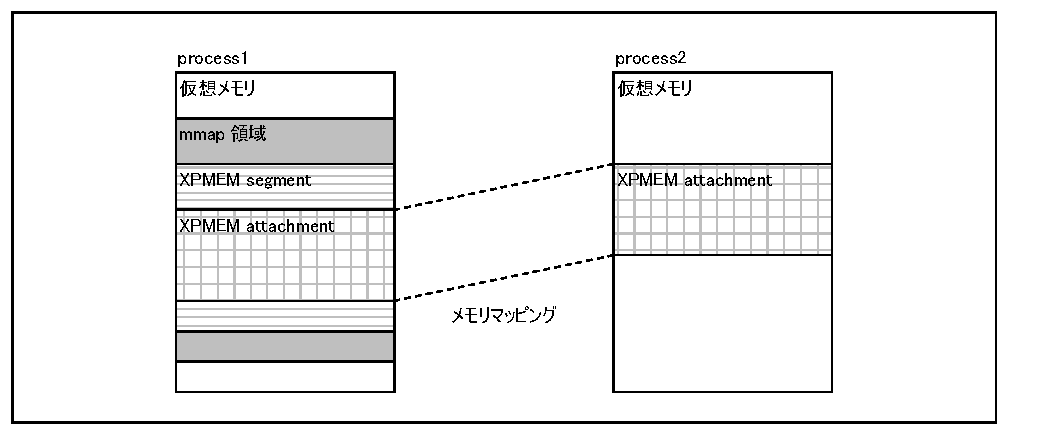
\includegraphics[scale=0.85]{figs/chap03_fig001.pdf}
  \caption{XPMEMのメモリマッピング}
  \label{figure:chap03_fig001}
\end{figure}
\FloatBarrier

\begin{figure}[!htb]
  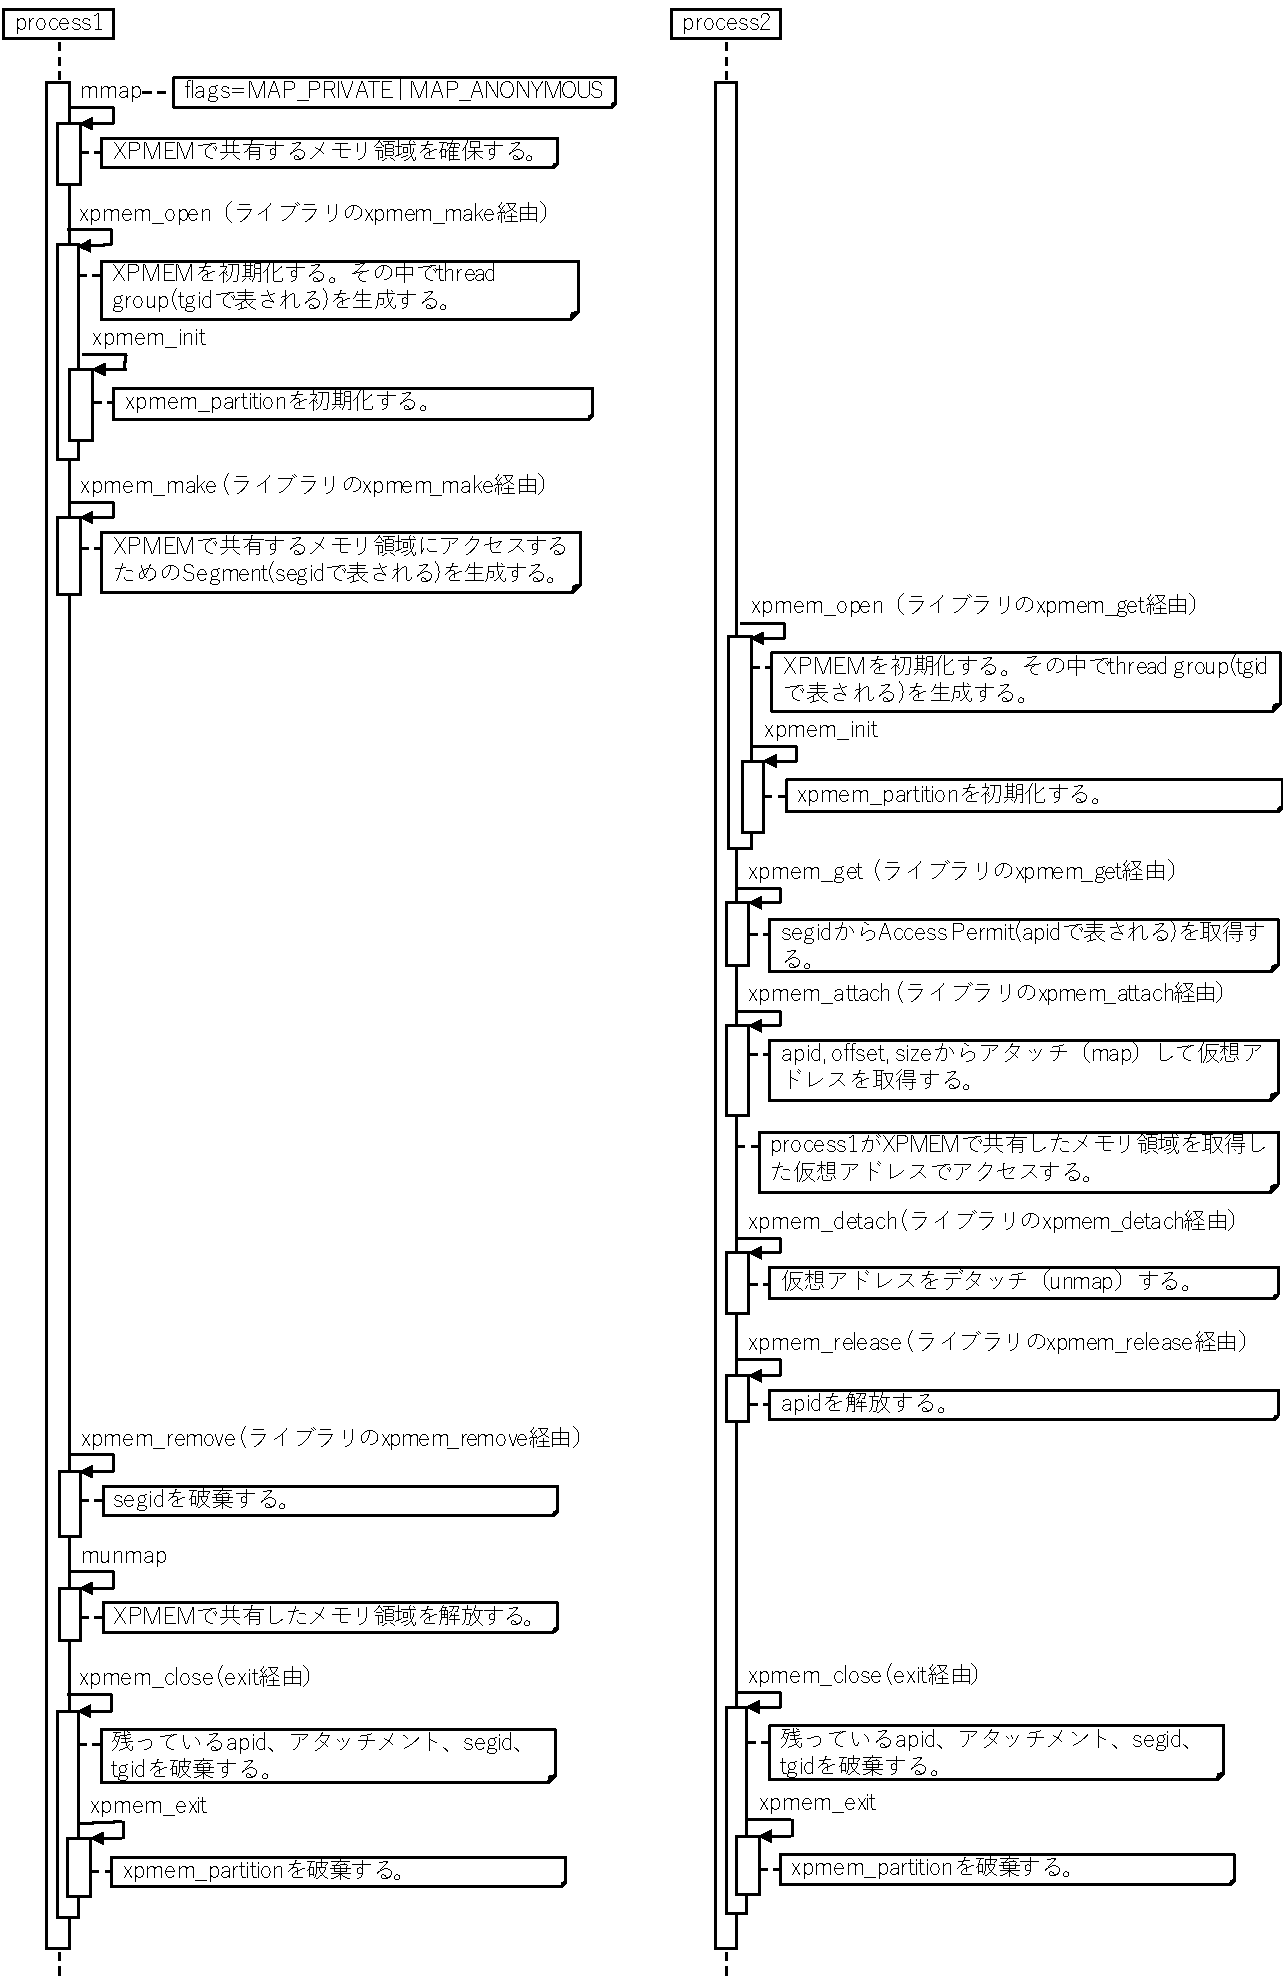
\includegraphics[width=0.9\linewidth]{figs/xpmem_flow.pdf}
  \caption{XPMEMの動作フロー}
  \label{figure:xpmem_flow}
\end{figure}
\FloatBarrier

XPMEMのメモリマッピングを図 \ref{figure:chap03_fig001} 、動作フローを図 \ref{figure:xpmem_flow} に示す。
%
XPMEMでは、プロセス(process1)がmmapしたメモリ領域から、xpmem\_make()で指定された領域をXPMEM segmentとして管理して他のプロセスからマップできるようにする。
%
マップしたいプロセス(process2)は、xpmem\_get()でアクセスパーミッションを得て、xpmem\_attach()で指定されたXPMEM segmentのメモリ領域をXPMEM attachmentとして管理して、マップする。
%
マップは、プロセス(process2)がXPMEM attachment領域にアクセスして、ページフォルトが発生した際、ページテーブルエントリが示す物理アドレスを、プロセス(process1)のXPMEM segment領域の物理アドレスに置き換えることで実現する。

XPMEMのデータ構造を生成・破棄する関数を図 \ref{figure:chap03_fig003} に示す。
\begin{figure}[ht]
  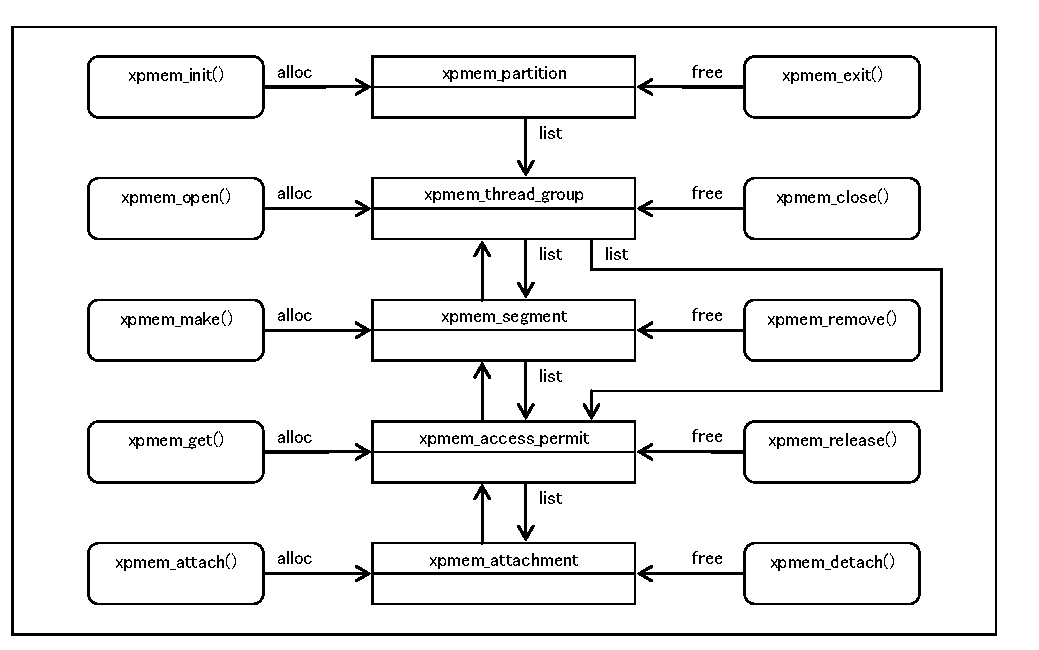
\includegraphics[scale=0.85]{figs/chap03_fig003.pdf}
  \caption{XPMEMのデータ構造を生成・破棄する関数}
  \label{figure:chap03_fig003}
\end{figure}
\FloatBarrier

XPMEMでは、以下のデータ構造を管理して機能を実現する。
\begin{enumerate}
  \item xpmem\_partition
  \item xpmem\_thread\_group
  \item xpmem\_segment
  \item xpmem\_access\_permit
  \item xpmem\_attachment
\end{enumerate}

XPMEMのデータ構造を図\ref{figure:xpmem_struct} に示す。
\begin{figure}[ht]
  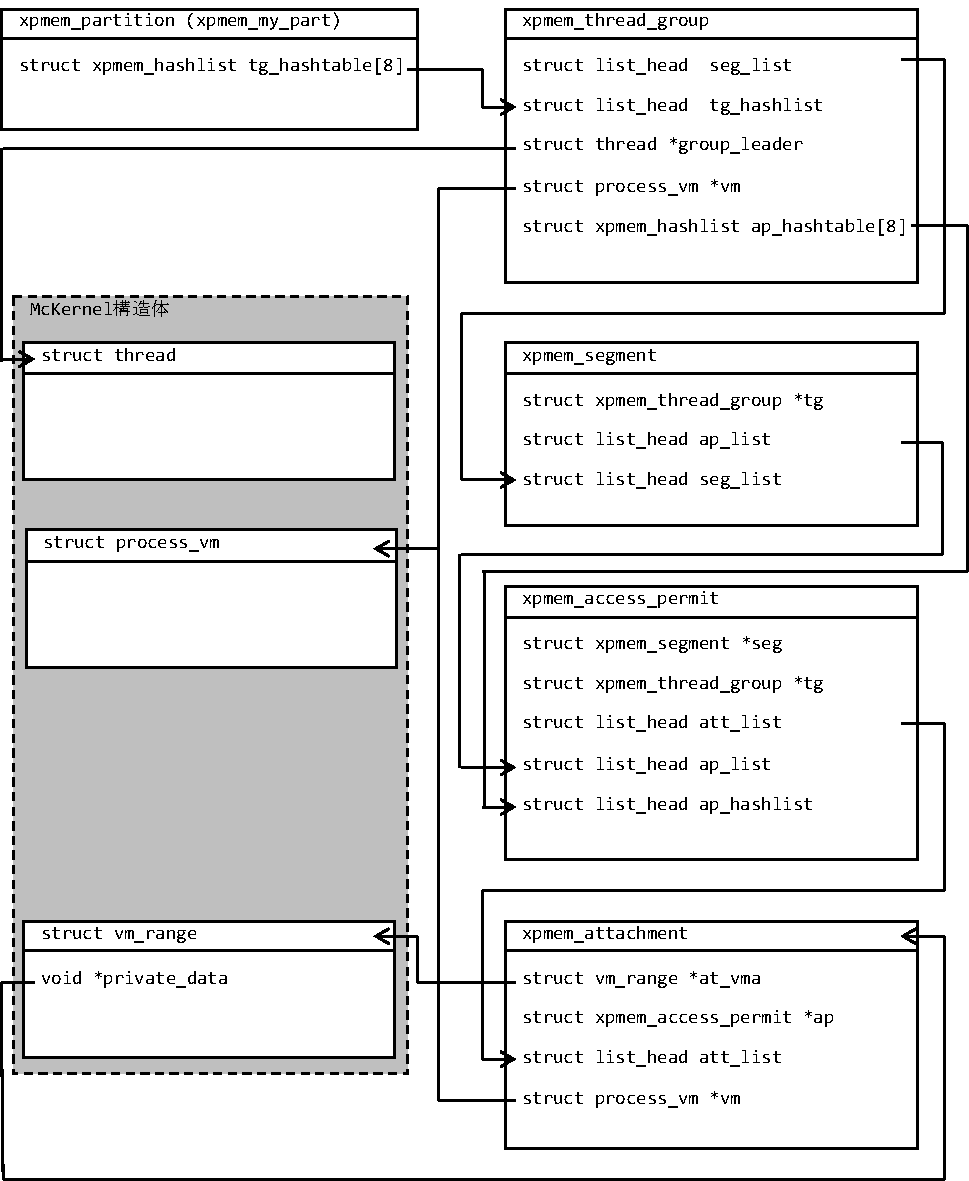
\includegraphics[width=0.9\linewidth]{figs/xpmem_struct.pdf}
  \caption{XPMEMのデータ構造}
  \label{figure:xpmem_struct}
\end{figure}
\FloatBarrier

\comment{
\subsection{McKernelのメモリ関連のデータ構造}
McKernelのメモリ関連のデータ構造を図 \ref{figure:chap03_fig005} に示す。
\begin{figure}[ht]
  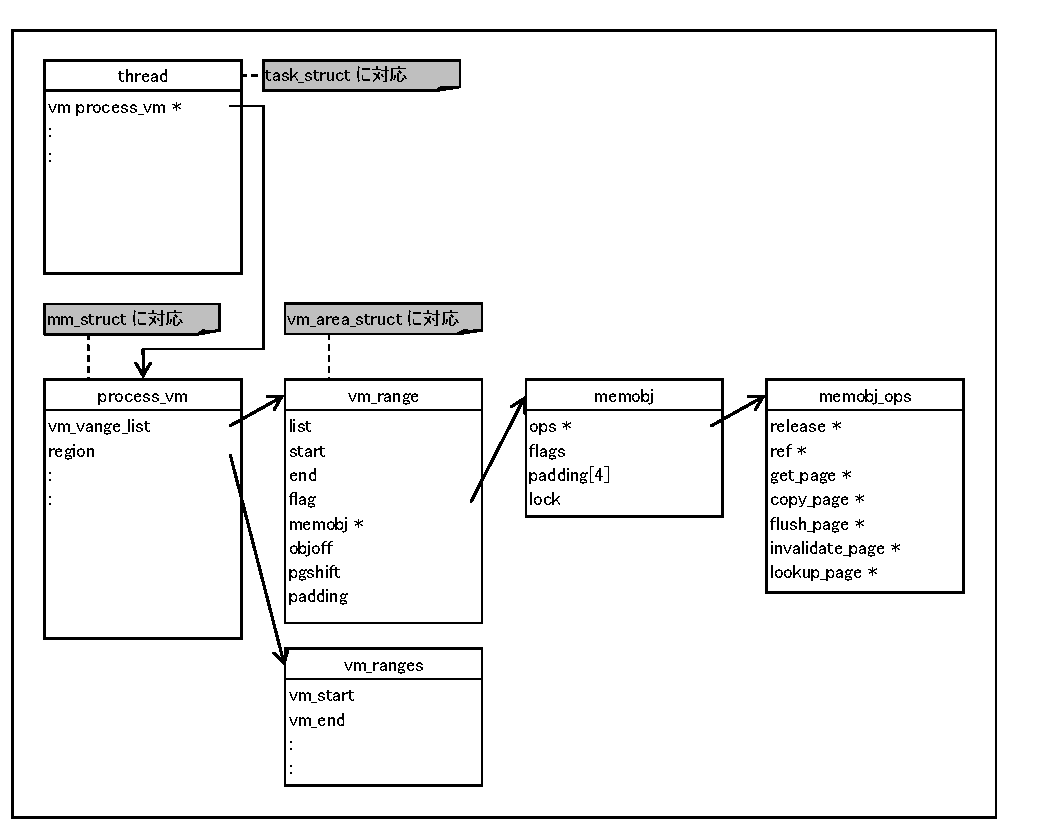
\includegraphics[scale=0.85]{figs/chap03_fig005.pdf}
  \caption{McKernelのメモリ関連のデータ構造}
  \label{figure:chap03_fig005}
\end{figure}

XPMEM移植の際には、McKernelの以下のデータ構造を使用する。
\begin{enumerate}
  \item thread\mbox{}\\
        Linuxのtask\_structに対応
  \item process\_vm\mbox{}\\
        Linuxのmm\_structに対応
  \item vm\_range\mbox{}\\
        Linuxのvm\_area\_structに対応
\end{enumerate}
}

\comment{
そして、McKernelの以下の関数の処理時にXPMEMの操作関数を呼び出すようにする。
\subsubsection{remove\_process\_memory\_range()}
remove\_process\_memory\_range()のfree\_process\_memory\_range()呼び出しの処理の前に、private\_dataが指定されている場合には、xpmem\_remove\_process\_memory\_range()を呼び出す。
\begin{verbatim}
...
if (range->private_data) {
        xpmem_remove_process_memory_range(vm, freerange);  <-- 追加
}

error = free_process_memory_range(vm, freerange);
...
\end{verbatim}

\subsubsection{do\_page\_fault\_process\_vm()}
do\_page\_fault\_process\_vm()のpage\_fault\_process\_memory\_range()呼び出しの処理を、private\_dataが指定されている場合には、xpmem\_fault\_process\_memory\_range()を呼び出すように切り替える。
\begin{verbatim}
...
if (!range->private_data) {
        error = page_fault_process_memory_range(
                        vm, range, fault_addr, reason);
} 
else {
        error = xpmem_fault_process_memory_range(        <-- 追加
                        vm, range, fault_addr, reason);
}
...
\end{verbatim}

また、プロセス終了時にデバイスファイルのクローズ処理されていない場合には、クローズ処理するようにrelease\_process\_vm()に組み込む。
\subsubsection{release\_process\_vm()}
\begin{verbatim}
...
irqstate = ihk_mc_spinlock_lock(&proc->mckfd_lock);
for (fdp = proc->mckfd; fdp; fdp = fdp->next) {
        if (fdp->close_cb) {
                fdp->close_cb(fdp, NULL);
        }
}
ihk_mc_spinlock_unlock(&proc->mckfd_lock, irqstate);
...
\end{verbatim}
}

以下、各関数のインターフェイスと動作を説明する。

\subsection{XPMEMデバイスファイルのオープン}
\subsubsection*{書式}{\quad}
\texttt{int xpmem\_open(ihk\_mc\_user\_context\_t *ctx)}

\subsubsection*{説明}{\quad}
xpmem\_openは、以下の処理を行う。
\begin{enumerate}
  \item XPMEMを初期化していない場合には、xpmem\_init()を呼び出してXPMEMを初期化する。
  \item fdを取得する必要があるが、/dev/xpmemデバイスファイルには影響を与えないように、do\_syscall()呼び出しで、/dev/nullデバイスファイルをオープンして、そのfdを使用する。fdがマイナス値の場合にはエラー値を戻す。
  \item \_\_xpmem\_open()を呼び出して、自プロセスのxpmem\_thread\_groupが生成されていなければ生成する。
  \item mckfdを生成して、初期設定する。
\end{enumerate}

\subsubsection*{戻り値}{\quad}
\begin{table}[!h]
\footnotesize
\begin{tabular}{|p{0.20\linewidth}|p{0.66\linewidth}|} \hline
0以上&ファイルディスクリプタ(正常終了)\\ \hline
\texttt{-EINVAL}&引数が無効である\\ \hline
\texttt{-ENOMEM}&十分な空きメモリ領域が無い\\ \hline
\end{tabular}
\vspace{-0em}
\end{table}
\FloatBarrier

\subsection{XPMEMデバイスファイルのioctl制御}
\subsubsection*{書式}{\quad}
\texttt{static int xpmem\_ioctl(struct mckfd *mckfd, ihk\_mc\_user\_context\_t *ctx)}

\subsubsection*{説明}{\quad}
xpmem\_ioctlは、以下の処理を行う。
\begin{enumerate}
\item cmdを処理する関数を呼び出す。
  \begin{enumerate}
  \item XPMEM\_CMD\_VERSION\mbox{}\\
        XPMEM\_CURRENT\_VERSIONを戻す。
  \item XPMEM\_CMD\_MAKE\mbox{}\\
        xpmem\_cmd\_makeデータを取得する。\\
        xpmem\_make()を呼び出す。\\
        xpmem\_cmd\_makeデータのsegidを設定する。
  \item XPMEM\_CMD\_REMOVE\mbox{}\\
        xpmem\_cmd\_removeデータを取得する。\\
        xpmem\_remove()を呼び出す。
  \item XPMEM\_CMD\_GET\mbox{}\\
        xpmem\_cmd\_getデータを取得する。\\
        xpmem\_get()を呼び出す。
        xpmem\_cmd\_getデータのapidを設定する。
  \item XPMEM\_CMD\_RELEASE\mbox{}\\
        xpmem\_cmd\_releaseデータを取得する。\\
        xpmem\_release()を呼び出す。
  \item XPMEM\_CMD\_ATTACH\mbox{}\\
        xpmem\_cmd\_attachデータを取得する。\\
        xpmem\_attach()を呼び出す。
        xpmem\_cmd\_attachデータのvaddrを設定する。
  \item XPMEM\_CMD\_DETACH\mbox{}\\
        xpmem\_cmd\_detachデータを取得する。\\
        xpmem\_detach()を呼び出す。
  \end{enumerate}
\end{enumerate}

\subsubsection*{戻り値}{\quad}
\begin{table}[!h]
\footnotesize
\begin{tabular}{|p{0.20\linewidth}|p{0.66\linewidth}|} \hline
0&正常終了\\ \hline
\texttt{-EFAULT}&アドレスが不正である\\ \hline
\texttt{-EINVAL}&引数が無効である\\ \hline
\end{tabular}
\vspace{-0em}
\end{table}
\FloatBarrier

\subsection{XPMEMデバイスファイルのクローズ}
\subsubsection*{書式}{\quad}
\texttt{static int xpmem\_close(struct mckfd *mckfd, ihk\_mc\_user\_context\_t *ctx)
}

\subsubsection*{説明}{\quad}
xpmem\_closeは、以下の処理を行う。
\begin{enumerate}
  \item pidからxpmem\_thread\_group(tg)を取得する。
  \item xpmem\_release\_aps\_of\_tg()を呼び出して、xpmem\_access\_permit、xpmem\_attachmentを破棄する。
  \item xpmem\_remove\_segs\_of\_tg()を呼び出して、xpmem\_segmentを破棄する。
  \item xpmem\_destroy\_tg()を呼び出して、xpmem\_thread\_groupを破棄する。
  \item /dev/xpmemをオープンしているプロセスが存在しない場合には、xpmem\_exit()を呼び出してXPMEMを終了する。
  \item xpmem\_open()でオープンした/dev/nullデバイスファイルについては、sys\_close()でクローズする。
\end{enumerate}

\subsubsection*{戻り値}{\quad}
\begin{table}[!h]
\footnotesize
\begin{tabular}{|p{0.20\linewidth}|p{0.66\linewidth}|} \hline
0&正常終了\\ \hline
\end{tabular}
\vspace{-0em}
\end{table}
\FloatBarrier

\subsection{XPMEMの初期化}
\subsubsection*{書式}{\quad}
\texttt{static int xpmem\_init(void)}

\subsubsection*{説明}{\quad}
xpmem\_initは、以下の処理を行う。
\begin{enumerate}
  \item xpmem\_partitionを生成して、初期設定する。
\end{enumerate}

\subsubsection*{戻り値}{\quad}
\begin{table}[!h]
\footnotesize
\begin{tabular}{|p{0.20\linewidth}|p{0.66\linewidth}|} \hline
0&正常終了\\ \hline
\texttt{-ENOMEM}&十分な空きメモリ領域が無い\\ \hline
\end{tabular}
\vspace{-0em}
\end{table}
\FloatBarrier

\subsection{XPMEMの終了}
\subsubsection*{書式}{\quad}
\texttt{static void xpmem\_exit(void)}

\subsubsection*{説明}{\quad}
xpmem\_exitは、以下の処理を行う。
\begin{enumerate}
  \item xpmem\_partitionを破棄する。
\end{enumerate}

\subsubsection*{戻り値}{\quad}
なし。

\subsection{\texttt{xpmem\_segment}の生成}
\subsubsection*{書式}{\quad}
\texttt{static int xpmem\_make(unsigned long vaddr,
        size\_t size,
        int permit\_type,
        void *permit\_value,
        xpmem\_segid\_t *segid\_p)
}

\subsubsection*{説明}{\quad}
xpmem\_makeは、以下の処理を行う。
\begin{enumerate}
  \item 自プロセスのxpmem\_thread\_groupを取得する。
  \item segidを算出する。
  \item xpmem\_segmentを生成して、初期設定する。
  \item segid\_pにsegidを設定する。
\end{enumerate}

\subsubsection*{戻り値}{\quad}
\begin{table}[!h]
\footnotesize
\begin{tabular}{|p{0.20\linewidth}|p{0.66\linewidth}|} \hline
0&正常終了\\ \hline
\texttt{-EINVAL}&引数が無効である\\ \hline
\texttt{-ENOMEM}&十分な空きメモリ領域が無い\\ \hline
\texttt{-XPMEM\_ERRNO\_NOPROC}&対象プロセスの情報が無い\\ \hline
\end{tabular}
\vspace{-0em}
\end{table}
\FloatBarrier

\subsection{\texttt{xpmem\_segment}の破棄}
\subsubsection*{書式}{\quad}
\texttt{static int xpmem\_remove(xpmem\_segid\_t segid)
}

\subsubsection*{説明}{\quad}
xpmem\_removeは、以下の処理を行う。
\begin{enumerate}
  \item segidからxpmem\_thread\_group(seg\_tg)を取得する。
  \item seg\_tg、segidからxpmem\_segmentを取得する。
  \item 取得したxpmem\_segmentを破棄する。
\end{enumerate}

\subsubsection*{戻り値}{\quad}
\begin{table}[!h]
\footnotesize
\begin{tabular}{|p{0.20\linewidth}|p{0.66\linewidth}|} \hline
0&正常終了\\ \hline
\texttt{-EACCES}&許可がない\\ \hline
\texttt{-EINVAL}&引数が無効である\\ \hline
\end{tabular}
\vspace{-0em}
\end{table}
\FloatBarrier

\subsection{\texttt{xpmem\_access\_permit}の生成}
\subsubsection*{書式}{\quad}
\texttt{static int xpmem\_get(xpmem\_segid\_t segid,
        int flags,
        int permit\_type,
        void *permit\_value,
        xpmem\_apid\_t *apid\_p)
}

\subsubsection*{説明}{\quad}
xpmem\_getは、以下の処理を行う。
\begin{enumerate}
  \item segidからxpmem\_thread\_group(seg\_tg)を取得する。
  \item seg\_tg、sigidからxpmem\_segmentを取得する。
  \item 自プロセスのxpmem\_thread\_group(ap\_tg)を取得する。
  \item ap\_tgからapidを算出する。apidがマイナス値の場合にはエラー値を戻す。
  \item xpmem\_access\_permitを生成して、初期設定する。
  \item apid\_pにapidを設定する。
\end{enumerate}

\subsubsection*{戻り値}{\quad}
\begin{table}[!h]
\footnotesize
\begin{tabular}{|p{0.20\linewidth}|p{0.66\linewidth}|} \hline
0&正常終了\\ \hline
\texttt{-EACCES}&許可がない\\ \hline
\texttt{-EINVAL}&引数が無効である\\ \hline
\texttt{-ENOMEM}&十分な空きメモリ領域が無い\\ \hline
\texttt{-XPMEM\_ERRNO\_NOPROC}&対象プロセスの情報が無い\\ \hline
\end{tabular}
\vspace{-0em}
\end{table}
\FloatBarrier

\subsection{\texttt{xpmem\_access\_permit}の破棄}
\subsubsection*{書式}{\quad}
\texttt{static int xpmem\_release(xpmem\_apid\_t apid)
}

\subsubsection*{説明}{\quad}
xpmem\_releaseは、以下の処理を行う。
\begin{enumerate}
  \item apidからxpmem\_thread\_group(ap\_tg)を取得する。
  \item ap\_tg、apidからxpmem\_access\_permitを取得する。
  \item 取得したxpmem\_access\_permitを破棄する。
\end{enumerate}

\subsubsection*{戻り値}{\quad}
\begin{table}[!h]
\footnotesize
\begin{tabular}{|p{0.20\linewidth}|p{0.66\linewidth}|} \hline
0&正常終了\\ \hline
\texttt{-EACCES}&許可がない\\ \hline
\texttt{-EINVAL}&引数が無効である\\ \hline
\end{tabular}
\vspace{-0em}
\end{table}
\FloatBarrier

\subsection{\texttt{xpmem\_attachment}の生成}
\subsubsection*{書式}{\quad}
\texttt{static int xpmem\_attach(struct mckfd *mckfd,
        xpmem\_apid\_t apid,
        off\_t offset,
        size\_t size,
        unsigned long vaddr,
        int fd,
        int att\_flags,
        unsigned long *at\_vaddr\_p)
}

\subsubsection*{説明}{\quad}
xpmem\_attachは、以下の処理を行う。
\begin{enumerate}
  \item apidからxpmem\_thread\_group(ap\_tg)を取得する。
  \item ap\_tg、apidからxpmem\_access\_permit(ap)を取得する。
  \item apからxpmem\_thread\_group(seg\_tg)、xpmem\_segment(seg)を取得する。
  \item xpmem\_attachmentを生成して、初期設定する。
  \item do\_mmap()を呼び出して、メモリ領域(at\_vaddr)を確保する。
  \item at\_vaddrからvm\_range(range)を取得する。
  \item range-\verb|>|private\_dataにxpmem\_attachmentを設定する。
\end{enumerate}

\comment{
McKernelのvm\_range構造体にXPMEMのデータを格納するためのprivate\_data変数を追加する。

vm\_range構造体を以下に示す。
\begin{verbatim}
struct vm_range {
        struct list_head list;
        unsigned long start, end;
        unsigned long flag;
        struct memobj *memobj;
        off_t objoff;
        int pgshift;    /* page size. 0 means THP */
        int padding;
        void *private_data;  <-- 追加
};
\end{verbatim}

vm\_range構造体のprivate\_dataには、xpmem\_attach()の処理時に生成するxpmem\_attachmentを設定する。
}

\subsubsection*{戻り値}{\quad}
\begin{table}[!h]
\footnotesize
\begin{tabular}{|p{0.20\linewidth}|p{0.66\linewidth}|} \hline
0&正常終了\\ \hline
\texttt{-EINVAL}&引数が無効である\\ \hline
\texttt{-ENOENT}&そのようなファイルやディレクトリは無い\\ \hline
\texttt{-ENOMEM}&十分な空きメモリ領域が無い\\ \hline
\end{tabular}
\vspace{-0em}
\end{table}
\FloatBarrier

\subsection{\texttt{xpmem\_attachment}の破棄}
\subsubsection*{書式}{\quad}
\texttt{static int xpmem\_detach(unsigned long at\_vaddr)
}

\subsubsection*{説明}{\quad}
xpmem\_detachは、以下の処理を行う。
\begin{enumerate}
  \item at\_vaddrからvm\_range(range)を取得する。
  \item range-\verb|>|private\_dataからxpmem\_attachmentを取得する。
  \item xpmem\_vm\_munmap()を呼び出して、以下の処理を行う。
  \begin{enumerate}
    \item ihk\_mc\_clear\_range()を呼び出して、メモリ領域を解放する。
    \item range-\verb|>|memobjを解放する。
    \item rangeを解放する。
  \end{enumerate}
  \item 取得したxpmem\_attachmentを破棄する。
\end{enumerate}

\subsubsection*{戻り値}{\quad}
\begin{table}[!h]
\footnotesize
\begin{tabular}{|p{0.20\linewidth}|p{0.66\linewidth}|} \hline
0&正常終了\\ \hline
\texttt{-EACCES}&許可がない\\ \hline
\texttt{-EINVAL}&引数が無効である\\ \hline
\end{tabular}
\vspace{-0em}
\end{table}
\FloatBarrier

\subsection{\texttt{vm\_range}のfault処理}
\subsubsection*{書式}{\quad}
\texttt{int xpmem\_fault\_process\_memory\_range(struct process\_vm *vm,
        struct vm\_range *vmr,
        unsigned long vaddr,
        uint64\_t reason)
}

\subsubsection*{説明}{\quad}
xpmem\_fault\_process\_memory\_rangeは、以下の処理を行う。
\begin{enumerate}
  \item vmr-\verb|>|private\_dataからxpmem\_attachment(att)を取得する。attがNULLの場合にはエラー値(-EFAULT)を戻す。
  \item attからxpmem\_access\_permit(ap)を取得する。
  \item apからxpmem\_thread\_group(ap\_tg)を取得する。ap-\verb|>|flagsまたはap\_tg-\verb|>|flagsがXPMEMi\_FLAG\_DESTROYINGの場合にはエラー値(-EFAULT)を戻す。
  \item apからxpmem\_segment(seg)を取得する。
  \item segからxpmem\_thread\_group(seg\_tg)を取得する。seg-\verb|>|flagsまたはseg\_tg-\verb|>|flagsがXPMEM\_FLAG\_DESTROYINGの場合にはエラー値(-ENOENT)を戻す。
  \item xpmem\_remap\_pte()を呼び出して、以下の処理を行う。
  \begin{enumerate}
    \item ihk\_mc\_pt\_lookup\_pte()を呼び出して、segのvaddrからpte\_t(seg\_pte)を取得する。
    \item ihk\_mc\_pt\_lookup\_pte()を呼び出して、vaddrからpte\_t(att\_pte)を取得する。
    \item ihk\_mc\_pt\_set\_pte()を呼び出して、att\_pteの物理アドレスをseg\_pteの物理アドレスに置き換える。
  \end{enumerate}
\end{enumerate}

\subsubsection*{戻り値}{\quad}
\begin{table}[!h]
\footnotesize
\begin{tabular}{|p{0.20\linewidth}|p{0.66\linewidth}|} \hline
0&正常終了\\ \hline
\texttt{-EFAULT}&アドレスが不正である\\ \hline
\texttt{-ENOENT}&そのようなファイルやディレクトリは無い\\ \hline
\end{tabular}
\vspace{-0em}
\end{table}
\FloatBarrier

\subsection{\texttt{vm\_range}の削除}
\subsubsection*{書式}{\quad}
\texttt{int xpmem\_remove\_process\_memory\_range(struct process\_vm *vm,
        struct vm\_range *vmr)
}

\subsubsection*{説明}{\quad}
xpmem\_remove\_process\_memory\_rangeは、以下の処理を行う。
\begin{enumerate}
  \item vmr-\verb|>|private\_dataからxpmem\_attachment(att)を取得する。
  \item attが指定されていた場合には、以下の処理を行う。
  \begin{enumerate}
    \item attを解放する。
    \item vmr-\verb|>|private\_dataにNULLを設定する。
  \end{enumerate}
\end{enumerate}

\subsubsection*{戻り値}{\quad}
\begin{table}[!h]
\footnotesize
\begin{tabular}{|p{0.20\linewidth}|p{0.66\linewidth}|} \hline
0&正常終了\\ \hline
\end{tabular}
\vspace{-0em}
\end{table}
\FloatBarrier

\section{\MODAUGS{ライブラリ切り替え}}
McKernelは、特定のパスについて、McKernel上に起動されたプロセスとLinux上に起動されたプロセスとに対して異なるファイルを見せる機能を提供する。これは、McKernelでの実行とLinuxでの実行とで異なるライブラリファイルをリンクせねばならない例外的なケース(例えば、第\ref{sec:uti}節で説明するUtility Thread Offloadingのライブラリ)で、ローダ/リンカに異なるファイルをリンクさせることを目的とする。

動作は以下の通り。IHK/McKernelのインストールディレクトリを\texttt{<install>}とする。
\begin{enumerate}
\item \texttt{unshare}コマンドを用いて\texttt{mcexec}のmount name spaceの設定を変更し、\texttt{mcexec}が\texttt{mcctrl}に依頼するbind mountが他プロセスからは見えないようにする。
\item \texttt{mcexec}が\texttt{mcctrl}に制御を移す。
\item \texttt{mcctrl}がユーザidをrootに変更し、\texttt{<install>/rootfs/}以下のファイルのそれぞれを\texttt{/}にbind mountする。
\item \texttt{mcctrl}がユーザidを元に戻し\texttt{mcexec}に制御を戻す。
\end{enumerate}

\section{\MODAUGS{状態監視}}
McKernelのハングアップ検知は以下のステップで実施される。
\begin{enumerate}
\item 運用ソフトウェアがIHKの関数を用いて通知のための\texttt{eventfd}を取得する。
\item McKernelがCPUごとの状態と状態遷移回数を記録する。
\item Linux上で動作するスレッド(\texttt{ihkmond})が上記の状態を監視し、2度同じ状態にあった場合、ハングアップと判断し、上記\texttt{eventfd}を用いて運用ソフトウェアに通知する。
\end{enumerate}
監視スレッドとハングアップ通知のインターフェイスは''IHK Specifications``に記載する。
本節では第2のステップを説明する。

状態と状態遷移回数の記録には\texttt{struct ihk\_os\_monitor}型の変数を用いる。
以下の説明ではこの型を持つ監視用の変数を\texttt{monitor}と呼ぶ。
\texttt{struct ihk\_os\_monitor}の関連部分は以下のように定義される。
%
\begin{verbatim}
struct ihk_os_monitor {
...
    int status;            /* OS状態 */
    unsigned long counter; /* OS状態が変化した回数 */
};
\end{verbatim}
%    int status_bak; /* OS状態の、前回の値 */
%    unsigned long ocounter; /* OS状態に入った回数の、前回の値 */

状態と状態遷移回数の記録の動作は以下の通り。
\begin{enumerate}
\item McKernelが以下のようにイベントに応じて状態と状態遷移回数を更新する。
\begin{itemize}
\item カーネルモードからユーザモードへの移行時:~\texttt{monitor.status}を\textttw{IHK\_OS\_MONITOR\_USER}に設定する。
\item ユーザモードからカーネルモードへの移行時:~\texttt{monitor.status}を\textttw{IHK\_OS\_MONITOR\_KERNEL}に設定し、\texttt{monitor.counter}をインクリメントする。
\item システムコール移譲時:~移譲開始直前に\texttt{monitor.status}の値を保存し、\textttw{IHK\_OS\_MONITOR\_KERNEL\_OFFLOAD}に設定する。また、移譲完了後に\texttt{monitoror.status}の値を保存しておいた値に戻し、\texttt{monitor.counter}をインクリメントする。
\item \texttt{rt\_sigtimedwait(), do\_sigsuspend(), futex(), nanosleep()}呼び出し時:~関数に入った直後に\texttt{monitor.status}を\textttw{IHK\_OS\_MONITOR\_KERNEL\_HEAVY}に設定する。なお、この状態に長時間滞在しても\MODAUG{ハングアップ}とは判定しない。
\item \texttt{idle()}呼び出し時:~関数に入った直後に\texttt{monitor.status}を\textttw{IHK\_OS\_MONITOR\_IDLE}に設定する。なお、この状態に長時間滞在しても\MODAUG{ハングアップ}とは判定しない。
その後、\texttt{cpu\_safe\_halt()}から復帰したタイミングで\texttt{monitor.status}を\textttw{IHK\_OS\_MONITOR\_KERNEL}に設定し、\texttt{monitor.counter}をインクリメントする。
\end{itemize}
\end{enumerate}

\section{\ADDAUGS{Non-Maskable Interrupt}}
Non-Maskable Interrupt (NMI)は対象CPUに以下の動作をさせるために用いられる。
\begin{itemize}
\item カーネルダンプの準備
\item 一時停止状態への遷移
\item 一時停止状態からの復帰
\end{itemize}

なお、カーネルダンプの準備については第\ref{sec:kdump}節に、一時停止状態への遷移及びそこからの復帰については第\ref{sec:halt}節に記載する。
\comment{
\item レジスタ値の保存
\item ダンプ対象ページの設定
\item \texttt{hlt}命令の実行
\item CPU状態の一時停止状態への遷移
\item \texttt{hlt}命令の実行
}

NMIの利用ステップは以下の通り。
\begin{enumerate}
\item McKernelがブート時に\texttt{ihk\_set\_nmi\_mode\_addr()}でNMIの動作を指定するMcKernelの変数\texttt{nmi\_mode}の物理アドレスをIHK-masterに伝える。
\item IHK-master driverが\texttt{nmi\_mode}の値を上記の動作のいずれかを示す値に設定し、\textttw{smp\_ihk\_os\_send\_nmi()}を呼び、各CPUにNMIを送る。
\item 各CPUが以下を実行する。
\begin{enumerate}
\item NMIを受けて、NMIハンドラ\texttt{nmi()}に制御を移す。
\item \texttt{nmi()}で\texttt{nmi\_mode}の値に応じた処理を行う。
\end{enumerate}
\end{enumerate}

以下、関連関数の動作を説明する。
\subsection{NMI動作設定}\label{sec:nmi_mode}
\subsubsection*{書式}{\quad} \texttt{int ihk\_set\_nmi\_mode\_addr(unsigned long addr)}
\subsubsection*{説明}{\quad} 
\texttt{addr}で指定される物理アドレスをNMIの動作を規定するMcKernelの変数\texttt{nmi\_mode}の物理アドレスとしてIHKに登録する。
こうすることで、IHKからMcKernelのNMIハンドラの動作を切り替えることができるようになる。
\texttt{nmi\_mode}の値とNMIハンドラの動作の対応は以下の通り。
\begin{table}[!h]
\footnotesize
\begin{tabular}{|p{0.10\linewidth}|p{0.76\linewidth}|} \hline
\multicolumn{1}{|c}{\textbf{値}}&\multicolumn{1}{|c|}{\textbf{動作}}\\ \hline \hline
0&
NMIハンドラで各CPUのカーネルダンプの準備を行う。
%詳細は第\ref{sec:kdump}節に記載する。
\\ \hline
1&NMIハンドラで各CPUの状態を一時停止状態へ遷移させる。
%詳細は第\ref{sec:halt}節に記載する。
\\ \hline
2&NMIハンドラで各CPUの状態を一時停止状態から復帰させる。
%詳細は第\ref{sec:halt}節に記載する。
\\ \hline
\end{tabular}
\vspace{-0em}
\end{table}
\FloatBarrier

\subsubsection*{戻り値}
\begin{table}[!h]
\footnotesize
\begin{tabular}{|p{0.20\linewidth}|p{0.66\linewidth}|} \hline
0&正常終了\\ \hline
\end{tabular}
\vspace{-0em}
\end{table}
\FloatBarrier

\subsection{NMI送信}
\subsubsection*{書式}{\quad} \texttt{static int smp\_ihk\_os\_send\_nmi(ihk\_os\_t ihk\_os, void *priv, int mode)}
\subsubsection*{説明}{\quad}
\texttt{nmi\_mode}を\texttt{mode}に設定した上で
%\texttt{\_\_default\_send\_IPI\_dest\_field()}により
各CPUにNMIを発行する。

\subsubsection*{戻り値}{\quad}
\begin{table}[!h]
\footnotesize
\begin{tabular}{|p{0.20\linewidth}|p{0.66\linewidth}|} \hline
0&正常終了\\ \hline
-EINVAL&エラー\\ \hline
\end{tabular}
\vspace{-0em}
\end{table}
\FloatBarrier

\subsection{NMIハンドラ}
\subsubsection*{書式}{\quad} \texttt{void nmi()}
\subsubsection*{説明}{\quad} 
\texttt{nmi\_mode}に指定された値に従った動作を行う。\texttt{nmi\_mode}の値と動作の対応は第\ref{sec:nmi_mode}に示す。
\comment{
\begin{table}[!h]
\footnotesize
\begin{tabular}{|p{0.10\linewidth}|p{0.76\linewidth}|} \hline
\multicolumn{1}{|c}{\textbf{値}}&\multicolumn{1}{|c|}{\textbf{動作}}\\ \hline \hline
0&カーネルダンプの準備を行う。
%レジスタ値をダンプ用のメモリ領域に記録し、\texttt{ihk\_mc\_query\_mem\_areas()}を呼んだ後、\texttt{hlt}命令を実行する。
\\ \hline
1&
%\texttt{freeze\_thaw()}を呼び、
CPUの状態を一時停止状態へ遷移させる。
%\texttt{hlt}命令を実行する。
\\ \hline
2&
%\texttt{freeze\_thaw()}を呼び、
CPUの状態を一時停止状態から復帰させる。
\\ \hline
\end{tabular}
\vspace{-0em}
\end{table}
\FloatBarrier
}

%\subsubsection*{戻り値}{\quad}
%なし

\section{\MODAUGS{全CPU一時停止}}\label{sec:halt}
\ADDAUG{McKernelは全CPUをFROZENと呼ぶ一時停止状態に遷移させる機能およびFROZENから復帰させる機能を提供する。
この機能と全CPUを低電力状態に遷移させる機能とを組み合わせることで、ジョブ単位での低電力状態への遷移とそこからの復帰を実現する。}

\begin{figure}[!ht]
  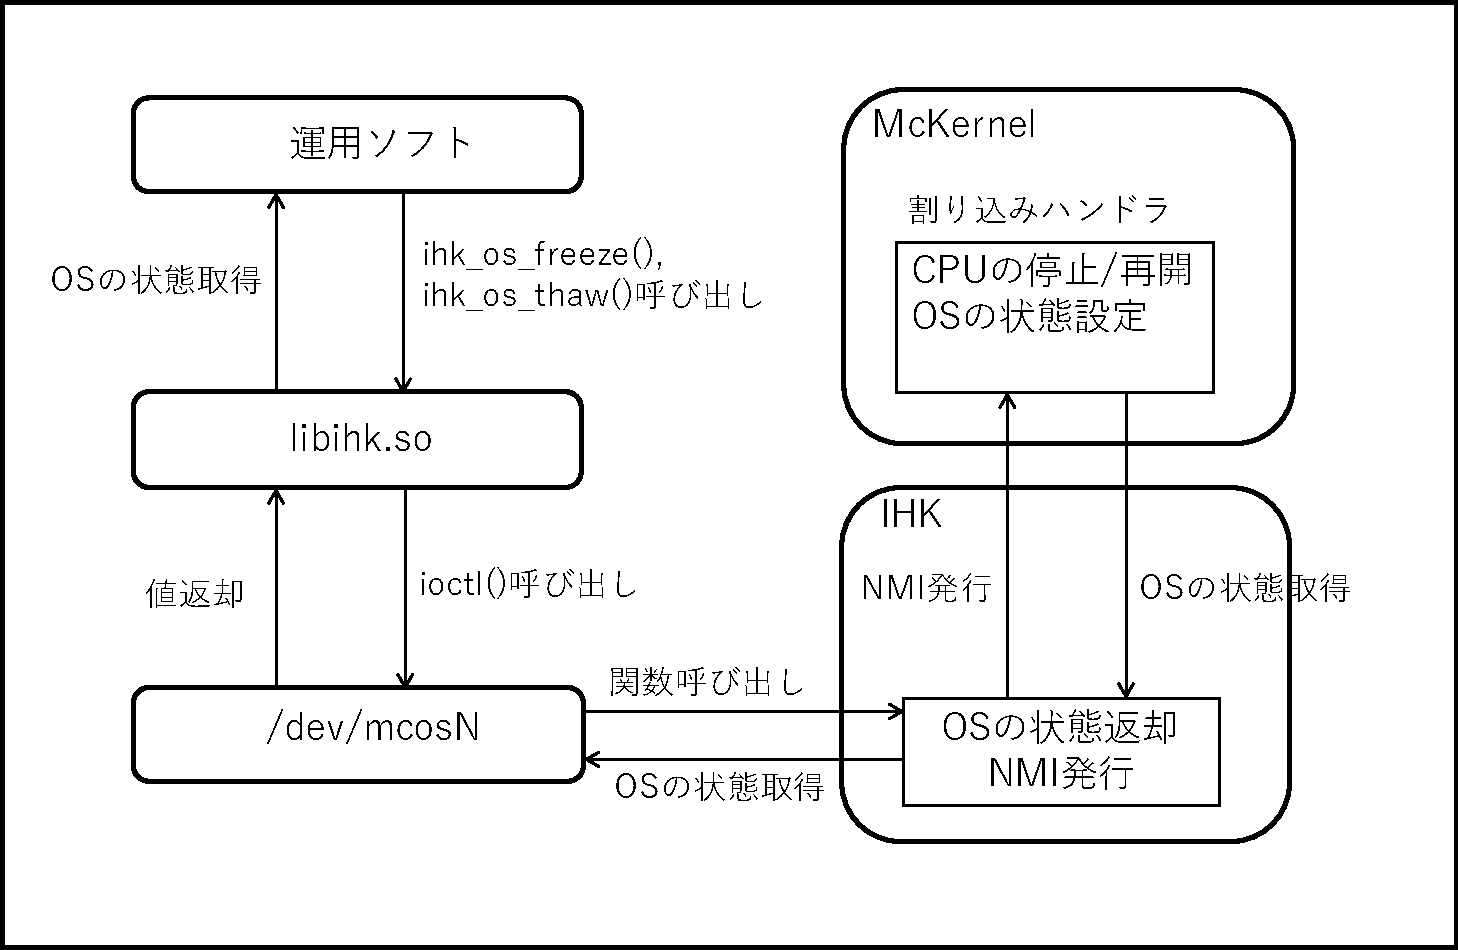
\includegraphics[scale=0.6,bb=0 0 720 540]{figs/freezer_structure.pdf}
  \caption{構成要素関連図}
  \label{figure:freezer_structure}
\end{figure}
\FloatBarrier
%
全CPU一時停止機能の構成を図\ref{figure:freezer_structure} に示す。

\begin{figure}[!ht]
  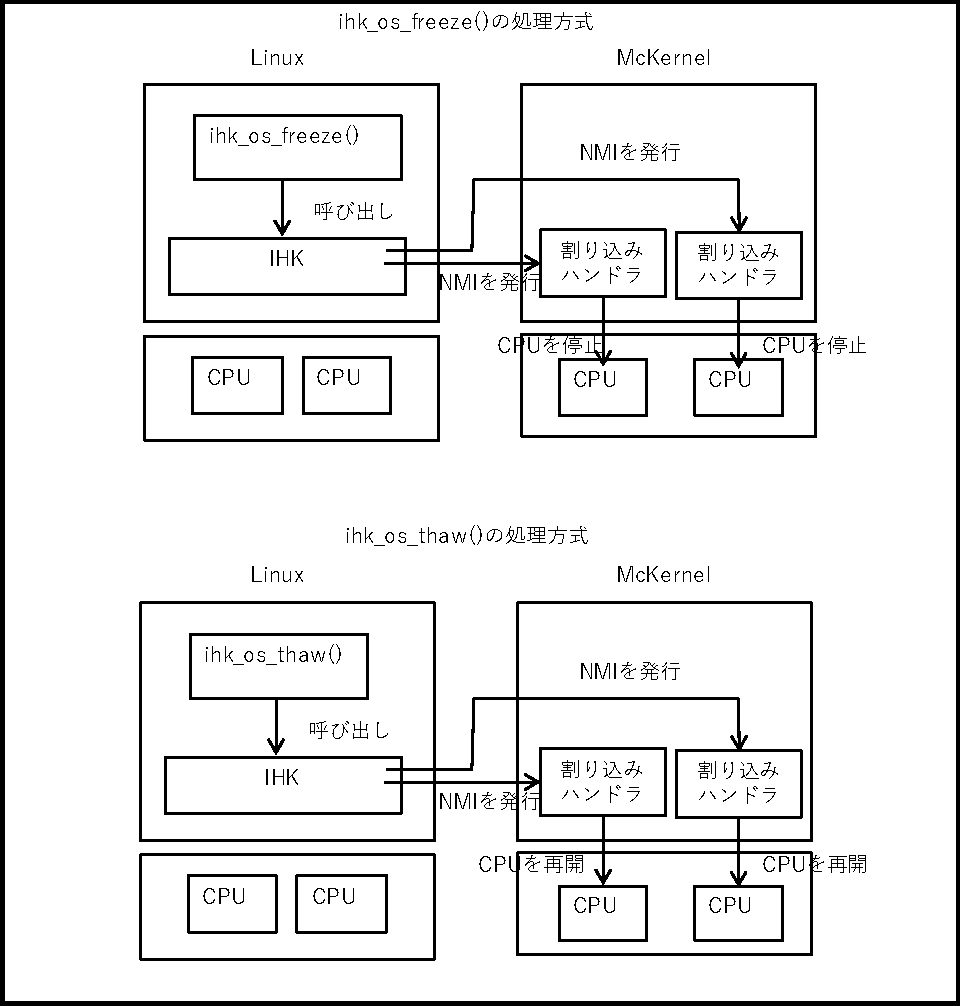
\includegraphics[scale=0.7,bb=0 0 720 540]{figs/freezer_flow.pdf}
  \caption{全CPU一時停止および一時停止からの復帰のフロー}
  \label{figure:chap02_fig002}
\end{figure}
\FloatBarrier
%
全CPU一時停止の動作を図\ref{figure:chap02_fig002}を用いて説明する。
\begin{enumerate}
\item バッチジョブスケジューラが\texttt{ihk\_os\_freeze()}経由で\texttt{IHK\_OS\_FREEZE}コマンドを指定して\texttt{ioctl()}を呼ぶ。
\item IHK-master coreが\texttt{\_\_ihk\_os\_freeze()}経由でIHK-master driverの\texttt{smp\_ihk\_os\_freeze()}を呼ぶ。
\item IHK-master driverが\texttt{nmi\_mode}に一時停止状態への遷移を示す値を設定し、\textttw{smp\_ihk\_os\_send\_nmi()}を呼び、各CPUにNMIを送る。
\item 各CPUが以下を実行する。
\begin{enumerate}
\item NMIを受けて、NMIハンドラ\texttt{nmi()}に制御を移す。
\item \texttt{nmi()}で\texttt{nmi\_mode}に設定された指示に従った処理を行う。この場合は一時停止状態への遷移であるため、\texttt{freeze\_thaw()}を呼ぶ。
\item \texttt{freeze\_thaw()}で\texttt{nmi\_mode}に設定された指示に従った処理を行う。この場合は一時停止状態への遷移であるため、\texttt{mod\_nmi\_ctx()}を用いて\texttt{iret}命令後のジャンプ先を\texttt{\_\_freeze()}にする。
\item \texttt{\_\_freeze()}は\texttt{freeze()}を呼び出す。\texttt{freeze()}は以下を実行する。
\begin{enumerate}
\item CPUの状態をバックアップ用変数に保持する。
\item CPUの状態を一時停止状態に設定する。
\item CPUを停止させる。\texttt{x86\_64}アーキでは\texttt{hlt}命令を実行する。
\end{enumerate}
\end{enumerate}
\end{enumerate}

一時停止からの復帰の動作を図\ref{figure:chap02_fig002}を用いて説明する。
\begin{enumerate}
\item バッチジョブスケジューラが\texttt{ihk\_os\_thaw()}経由で\texttt{IHK\_OS\_THAW}コマンドを指定して\texttt{ioctl()}を呼ぶ。
\item IHK-master coreが\texttt{\_\_ihk\_os\_thaw()}経由でIHK-master driverの\texttt{smp\_ihk\_os\_thaw()}を呼ぶ。
\item IHK-master driverが\texttt{nmi\_mode}に一時停止状態からの復帰を示す値を設定し、\textttw{smp\_ihk\_os\_send\_nmi()}を呼び、各CPUにNMIを送る。
\item 各CPUが以下を実行する。
\begin{enumerate}
\item NMIを受けて、NMIハンドラ\texttt{nmi()}に制御を移す。
\item \texttt{nmi()}で\texttt{nmi\_mode}に設定された指示に従った処理を行う。この場合は一時停止状態からの復帰であるため、\texttt{freeze\_thaw()}を呼ぶ。
\item \texttt{freeze\_thaw()}で\texttt{nmi\_mode}に設定された指示に従った処理を行う。この場合は一時停止状態からの復帰であるため、CPUの状態をバックアップ用変数を用いて復元する。
\end{enumerate}
\end{enumerate}

以下、関連関数のインターフェイスと動作を説明する。

\comment{
\subsection{ioctl()に渡すリクエスト}
ioctl()に渡すリクエスト用の定数に、\texttt{IHK\_OS\_FREEZE, IHK\_OS\_THAW}を追加する。
\begin{verbatim}
#define IHK_OS_RELEASE_CPU            0x112a23
#define IHK_OS_ASSIGN_MEM             0x112a24
#define IHK_OS_RELEASE_MEM            0x112a25
#define IHK_OS_QUERY_CPU              0x112a26
#define IHK_OS_QUERY_MEM              0x112a27
#define IHK_OS_FREEZE                 0x112a30
#define IHK_OS_THAW                  0x112a31
\end{verbatim}

\subsection{列挙型ihk\_os\_status}
IHKで保持するOSの状態を示す列挙型ihk\_os\_statusの定数に、IHK\_OS\_STATUS\_FROZENを追加する。
\begin{verbatim}
enum ihk_os_status {
    IHK_OS_STATUS_NOT_BOOTED,
    IHK_OS_STATUS_BOOTING,
    IHK_OS_STATUS_BOOTED,    /* OS booted and acked */
    IHK_OS_STATUS_READY,     /* OS is ready and fully functional */
    IHK_OS_STATUS_SHUTDOWN,  /* OS is shutting down */
    IHK_OS_STATUS_STOPPED,   /* OS stopped successfully */
    IHK_OS_STATUS_FAILED,    /* OS panics or failed to boot */
    IHK_OS_STATUS_HUNGUP,    /* OS is hungup */
    IHK_OS_STATUS_FROZEN,    /* OS is frozen */
};
\end{verbatim}

\subsection{列挙型ihk\_special\_addr\_type}
列挙型ihk\_special\_addr\_typeに、NMIのモードを定義する定数IHK\_SPADDR\_NMI\_MODEを追加する。
\begin{verbatim}
enum ihk_special_addr_type {
    IHK_SPADDR_KMSG = 1,
    IHK_SPADDR_MIKC_QUEUE_RECV = 2,
    IHK_SPADDR_MIKC_QUEUE_SEND = 3,
    IHK_SPADDR_MONITOR = 4,
    IHK_SPADDR_NMI_MODE = 5,
\end{verbatim}
\begin{verbatim}
}
\end{verbatim}

\subsection{構造体ihk\_os\_monitor}
CPUを停止した時のCPUの状態を保持するため、メンバー変数status\_bakを追加する。
\begin{verbatim}
struct ihk_os_monitor {
    int status;
    int status_bak;
    unsigned long counter;
    unsigned long ocounter;
    unsigned long user_tsc;
    unsigned long system_tsc;
};
\end{verbatim}

\subsection{構造体smp\_boot\_param}
構造体smp\_boot\_paramに、NMI処理用のメンバー変数nmi\_mode\_addrを追加する。
\begin{verbatim}
struct smp_boot_param {
        unsigned long start, end;
        unsigned long status;
        unsigned long msg_buffer;
        unsigned long msg_buffer_size;
        unsigned long mikc_queue_recv, mikc_queue_send;

        unsigned long monitor;
        unsigned long monitor_size;

        unsigned long nmi_mode_addr;

        unsigned long dma_address;
        unsigned long ident_table;
        unsigned long ns_per_tsc;
        unsigned long boot_sec;
        unsigned long boot_nsec;
        unsigned int ihk_ikc_irq;
        unsigned int ihk_ikc_irq_apicid;
        char kernel_args[256];
        int nr_cpus;
        int nr_numa_nodes;
        int nr_memory_chunks;
};
\end{verbatim}

\subsection{構造体ihk\_os\_ops}
構造体ihk\_os\_opsに、CPU停止処理、およびCPU再開処理の関数登録用にメンバー変数freeze、およびthawを追加し、呼び出す関数を追加する。
\begin{verbatim}
static struct ihk_os_ops smp_ihk_os_ops = {
    .load_mem = smp_ihk_os_load_mem,
    .load_file = smp_ihk_os_load_file,
    .boot = smp_ihk_os_boot,
    .shutdown = smp_ihk_os_shutdown,
    .alloc_resource = smp_ihk_os_alloc_resource,
    .query_status = smp_ihk_os_query_status,
    .wait_for_status = smp_ihk_os_wait_for_status,
    .set_kargs = smp_ihk_os_set_kargs,
    .dump = smp_ihk_os_dump,
    .issue_interrupt = smp_ihk_os_issue_interrupt,
    .map_memory = smp_ihk_os_map_memory,
    .unmap_memory = smp_ihk_os_unmap_memory,
    .register_handler = smp_ihk_os_register_handler,
    .unregister_handler = smp_ihk_os_unregister_handler,
    .get_special_addr = smp_ihk_os_get_special_addr,
    .debug_request = smp_ihk_os_debug_request,
    .get_memory_info = smp_ihk_os_get_memory_info,
    .get_cpu_info = smp_ihk_os_get_cpu_info,
    .assign_cpu = smp_ihk_os_assign_cpu,
    .release_cpu = smp_ihk_os_release_cpu,
    .query_cpu = smp_ihk_os_query_cpu,
    .assign_mem = smp_ihk_os_assign_mem,
    .release_mem = smp_ihk_os_release_mem,
    .query_mem = smp_ihk_os_query_mem,
    .freeze = smp_ihk_os_freeze,
    .thaw = smp_ihk_os_thaw,
};
\end{verbatim}

\subsection{定数値の追加}
構造体monitorのメンバー変数statusが取りうる定数値として下記を追加する。
\begin{itemize}
\item IHK\_OS\_MONITOR\_KERNEL\_FROZEN
\item IHK\_OS\_MONITOR\_KERNEL\_THAW
\end{itemize}
\begin{verbatim}
#define IHK_OS_MONITOR_NOT_BOOT 0
#define IHK_OS_MONITOR_IDLE 1
#define IHK_OS_MONITOR_USER 2
#define IHK_OS_MONITOR_KERNEL 3
#define IHK_OS_MONITOR_KERNEL_HEAVY 4
#define IHK_OS_MONITOR_KERNEL_OFFLOAD 5
#define IHK_OS_MONITOR_KERNEL_FROZEN 9
#define IHK_OS_MONITOR_KERNEL_THAW 10
#define IHK_OS_MONITOR_PANIC 99
\end{verbatim}
}

\comment{
\subsection{ihk\_host\_os\_ioctl}
\subsubsection*{書式}{\quad} \texttt{static long ihk\_host\_os\_ioctl(struct file *file, unsigned int request, unsigned long arg)}
\subsubsection*{修正内容}{\quad} ihk\_host\_os\_ioctl()では以下を修正する。
ioctlで与えた定数の分岐にIHK\_OS\_FREEZE、及びIHK\_OS\_THAWを追加する。
\begin{verbatim}
        case IHK_OS_DUMP:
                ret = __ihk_os_dump(data, (char __user *)arg);
                break;
\end{verbatim}
\begin{verbatim}
        case IHK_OS_FREEZE:
                ret = __ihk_os_freeze();
                break;
        case IHK_OS_THAW:
                ret = __ihk_os_thaw();
                break;
\end{verbatim}
\begin{verbatim}
        default:
\end{verbatim}
}

\subsection{一時停止指示(IHK-master core)}
\subsubsection*{書式}{\quad} \texttt{static int \_\_ihk\_os\_freeze(struct ihk\_host\_linux\_os\_data *data)}
\subsubsection*{説明}{\quad} 
アーキ依存の一時停止指示関数を呼ぶ。\texttt{smp-x86}では\texttt{smp\_ihk\_os\_freeze()}を呼び出す。
\subsubsection*{戻り値}{\quad}
\begin{table}[!h]
\footnotesize
\begin{tabular}{|p{0.20\linewidth}|p{0.66\linewidth}|} \hline
0&正常終了\\ \hline
\end{tabular}
\vspace{-0em}
\end{table}
\FloatBarrier

\subsection{一時停止からの復帰指示(IHK-master core)}
\subsubsection*{書式}{\quad} \texttt{static int \_\_ihk\_os\_thaw(struct ihk\_host\_linux\_os\_data *data)}
\subsubsection*{説明}{\quad} 
アーキ依存の一時停止からの復帰指示関数を呼ぶ。\texttt{smp-x86}では\texttt{smp\_ihk\_os\_thaw()}を呼び出す。
\subsubsection*{戻り値}{\quad}
\begin{table}[!h]
\footnotesize
\begin{tabular}{|p{0.20\linewidth}|p{0.66\linewidth}|} \hline
0&正常終了\\ \hline
\end{tabular}
\vspace{-0em}
\end{table}
\FloatBarrier

\comment{
\subsection{smp\_ihk\_os\_dump}
\subsubsection*{書式}{\quad} \texttt{static int smp\_ihk\_os\_dump(ihk\_os\_t ihk\_os, void *priv, dumpargs\_t *args)}
\subsubsection*{説明}{\quad}
NMIの発行処理をsmp\_ihk\_os\_send\_nmi()に移動した。smp\_ihk\_os\_send\_nmi()を、NMIのモード0(ダンプ取得を意味する)を引数として呼び出す。
\subsubsection*{戻り値}{\quad}
\begin{table}[!h]
\footnotesize
\begin{tabular}{|p{0.20\linewidth}|p{0.66\linewidth}|} \hline
0&正常終了\\ \hline
\end{tabular}
\vspace{-0em}
\end{table}
\FloatBarrier
}

\subsection{一時停止指示(IHK-master driver)}
\subsubsection*{書式}{\quad} \texttt{static int smp\_ihk\_os\_freeze(ihk\_os\_t ihk\_os, void *priv)}
\subsubsection*{説明}{\quad} 
\texttt{smp\_ihk\_os\_send\_nmi()}を呼び出して各CPUにNMIを送り、CPUの状態を一時停止状態へ遷移させ、またCPUをNMIを受けるまで停止させる。
\subsubsection*{戻り値}{\quad}
\begin{table}[!h]
\footnotesize
\begin{tabular}{|p{0.20\linewidth}|p{0.66\linewidth}|} \hline
0&正常終了\\ \hline
\end{tabular}
\vspace{-0em}
\end{table}
\FloatBarrier

\subsection{一時停止からの復帰指示 (IHK-master driver)}
\subsubsection*{書式}{\quad} \texttt{static int smp\_ihk\_os\_thaw(ihk\_os\_t ihk\_os, void *priv)}
\subsubsection*{説明}{\quad} 
smp\_ihk\_os\_send\_nmi()を呼び出して各CPUにNMIをを送り、NMI待ちで停止しているCPUの処理を再開させ、またCPUの状態を元の状態に戻す。
\subsubsection*{戻り値}{\quad}
\begin{table}[!h]
\footnotesize
\begin{tabular}{|p{0.20\linewidth}|p{0.66\linewidth}|} \hline
0&正常終了\\ \hline
\end{tabular}
\vspace{-0em}
\end{table}
\FloatBarrier

%%%%%%%%%%%%%%%%%%%%%%%%

\subsection{一時停止および一時停止からの復帰指示}
\subsubsection*{書式}{\quad} \texttt{long freeze\_thaw(void *nmi\_ctx)}
\subsubsection*{説明}{\quad} 
\begin{enumerate}
\item 変数\texttt{nmi\_mode}が一時停止状態への遷移を意味する場合、\texttt{mod\_nmi\_ctx()}を呼び出すことで\texttt{\_\_freeze()}を呼び出し、CPUの状態を一時停止状態に遷移させ、またCPUをNMIを受けるまで停止させる。
\item 変数\texttt{nmi\_mode}が一時停止状態からの復帰を意味する場合、CPUの状態を一時停止前の状態に戻す。
\end{enumerate}
\subsubsection*{戻り値}{\quad}
\begin{table}[!h]
\footnotesize
\begin{tabular}{|p{0.20\linewidth}|p{0.66\linewidth}|} \hline
0&一時停止を行った\\\hline
1&一時停止からの復帰を行った\\\hline
\end{tabular}
\vspace{-0em}
\end{table}
\FloatBarrier

\subsection{NMIハンドラからの復帰時の指定関数へのジャンプ設定}
\subsubsection*{書式}{\quad} \texttt{void mod\_nmi\_ctx(void *nmi\_ctx, void (*func)())}
\subsubsection*{説明}{\quad} 
NMIハンドラからの復帰時(\texttt{x86\_64}アーキテクチャでは\texttt{iret}命令実行時)に割り込み発生命令に戻らず、\texttt{func}で指定した、NMI受け付けが必要な関数にジャンプするようにスタックの内容を変更する。
このような処理が必要なのは、NMIハンドラ内ではNMIを受け付けないためである。
\texttt{func}に\texttt{\_\_freeze()}を指定することで、CPUをNMI待ちの状態で停止させることができる。

\comment{
\begin{figure}[!ht]
  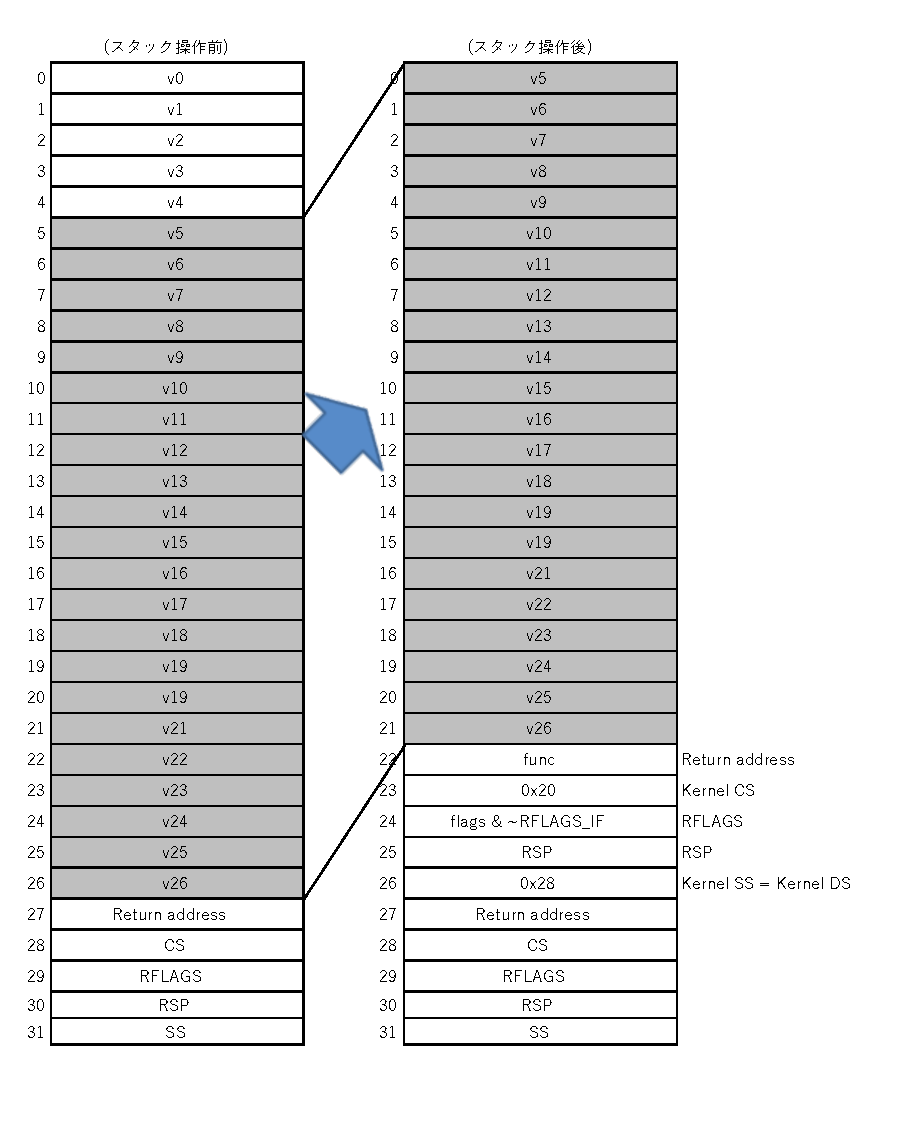
\includegraphics[width=0.9\linewidth]{figs/mod_nmi_ctx.pdf}
  \caption{スタック操作図}
  \label{figure:mod_nmi_ctx}
\end{figure}
\FloatBarrier
%
\texttt{x86\_64}アーキの場合のスタック操作を図\ref{figure:mod_nmi_ctx}を用いて説明する。
NMIハンドラから抜ける際に実行される\texttt{iret}命令は図の第22番目から第26番目をエントリを参照するため、ここに\texttt{func}のアドレス、コードセグメント、フラグ値、スタックポインタの値、スタックセグメントを書き込むことで、\texttt{\_\_freeze}にジャンプする。\texttt{\_\_freeze}によって実行される\texttt{iret}命令は図の第27目から第31番めのエントリ、すなわちスタック操作前の復帰用情報を参照してNMI発生時に実行していた命令から実行を再開する。
}

\subsection{一時停止指示(ラッパー)}
\subsubsection*{書式}{\quad} \texttt{void \_\_freeze()}
\subsubsection*{説明}{\quad} 
\texttt{freeze()}を呼び出してCPUを一時停止させ、その後割り込みハンドラから復帰する。
\texttt{x86\_64}アーキでは割り込みハンドラからの復帰には\texttt{iret}命令を用いる。

\subsection{一時停止指示}
\subsubsection*{書式}{\quad} \texttt{void freeze()}
\subsubsection*{説明}{\quad} 
ステップは以下の通り。
\begin{enumerate}
\item CPU状態を保存する。
\item CPU状態を\texttt{IHK\_OS\_MONITOR\_KERNEL\_FROZEN}に遷移させる。
\item \texttt{cpu\_halt()}を呼びCPUを停止させる。なお、CPUはNMIを受けると処理を再開する。
\item CPUが処理を再開した後、CPU状態を保存しておいた値に戻す。
\end{enumerate}

%==============================================================================
\section{\MODAUGS{カーネルダンプ}}\label{sec:kdump}
%==============================================================================
カーネルダンプの採取と解析のステップは以下の通り。
\begin{enumerate}
\item 以下のいずれかの方法でダンプファイルを作成する。
\begin{enumerate}
\item IHKの関数\texttt{ihk\_os\_makedumpfile()}またはIHKのコマンド\texttt{ihkosctl}を用いて、McKernel形式のダンプファイルを作成する(以降、McKernel主導ダンプと呼ぶ)。
\item Linuxのpanicを契機に\texttt{makedumpfile}形式のダンプファイルを作成する。また、コマンド\texttt{vmcore2mckdump}を用いてMcKernel形式に変換する(以降、Linux主導ダンプと呼ぶ)。
\end{enumerate}
\item eclairと呼ぶコマンドを用いてダンプファイルを解析する。
\end{enumerate}

\comment{
以下、それぞれのステップの動作を説明する。

\MODAUG{IHKの関数あるいはコマンドを用いたダンプファイル作成の動作ステップは以下の通り。}
\begin{enumerate}
\item IHKが\texttt{ihk\_os\_makedumpfile()}または\texttt{ihkosctl <os\_index> dump}コマンドによってMcKernelにダンプを指示する。同時にダンプ対象ページ種を指定する。
\item IHKが各CPUにNMIを送り、McKernelのダンプ準備関数を呼び出す。
\item McKernelのダンプ準備関数が以下の処理を行う。
\begin{enumerate}
\item スレッド情報を所定のメモリ領域に保存し、CPUを停止する。
\item プロセスのページテーブルとメモリアロケータを解析することでダンプ対象ページリストをIHKのメモリに記録する。
\end{enumerate}
\item IHKがダンプ対象ページリストを参照して物理ページをファイルへ出力する。
\end{enumerate}

\MODAUG{Linuxでpanicが起きた際のダンプ生成の動作ステップは以下の通り。}
\begin{enumerate}
\item \MODJULTWO{運用ソフトがMcKernelのカーネル引数を用いてダンプ対象とするページ種の設定を行う。}
\item \texttt{mcctrl}が\texttt{panic\_notifier()}に\texttt{mcctrl}のダンプ準備関数を登録する。
\item Linuxがpanicを起こし、\texttt{mcctrl}のダンプ準備関数を呼び出す。
\item \texttt{mcctrl}のダンプ準備関数が、各CPUにNMIを送り、上記で説明したMcKernelのダンプ準備関数を呼び出す。
\item McKernelのダンプ準備関数をが、スレッド情報の保存、CPUの停止、ダンプ対象ページリストの作成を行う。
\item \texttt{mcctrl}のダンプ準備関数が、タンプ対象ページリストを用いて、ダンプ対象外ページがLinuxからanonyous pageに見えるようにする。これは、対応するLinuxの\texttt{struct page}のフィールドを操作することで行う。
\item Linuxが\texttt{makedumpfile}でダンプを行う。\texttt{makedumpfile}でanonymous pageをダンプしない指定を行うことで、ダンプ対象ページリストにあるページのみファイルに出力されるようにする。
\end{enumerate}

makedumpfile形式からMcKernel形式への変換機能の動作ステップは以下の通り。
\begin{enumerate}
\item Linuxのcrash utility(以下、crashと呼ぶ)がダンプファイルを読み込む。
\item crashがIHK-master coreおよびIHK-master driverのシンボル情報を読み込む。
\item crashが変換プラグインを読み込む。
\item 変換プラグインが上記シンボル情報を用いてMcKernelに割り当てられた物理アドレス領域を特定する。
\item 変換プラグインが上記物理アドレス領域情報を用いてダンプファイルからMcKernelに関するヘッダやセクションを取り出し、必要に応じてeclair形式に変換しファイルに出力する。
\end{enumerate}

eclairの動作は以下の通り。
\begin{enumerate}
\item ユーザが\texttt{eclair}をLinux上に起動する。
\item \texttt{eclair}はgdbフロントエンドとgdbエージェントをLinux上に起動する。
\item ユーザはgdbフロントエンドに解析コマンドを入力する。
\item gdbフロントエンドはコマンドを受け取ると、remote serial protocolと呼ばれるプロトコルを用いてgdbエージェントに指示を出し、gdbエージェントから解析結果を受け取る。
\end{enumerate}
}

以下、詳細を説明する。

\subsection{\MODAUGS{全体の処理の流れ}}
McKernel主導ダンプの場合のダンプ採取機能とダンプ形式変換機能の処理の流れを図\ref{figure:chap01_fig006}を用いて説明する。
\begin{figure}[!ht]
  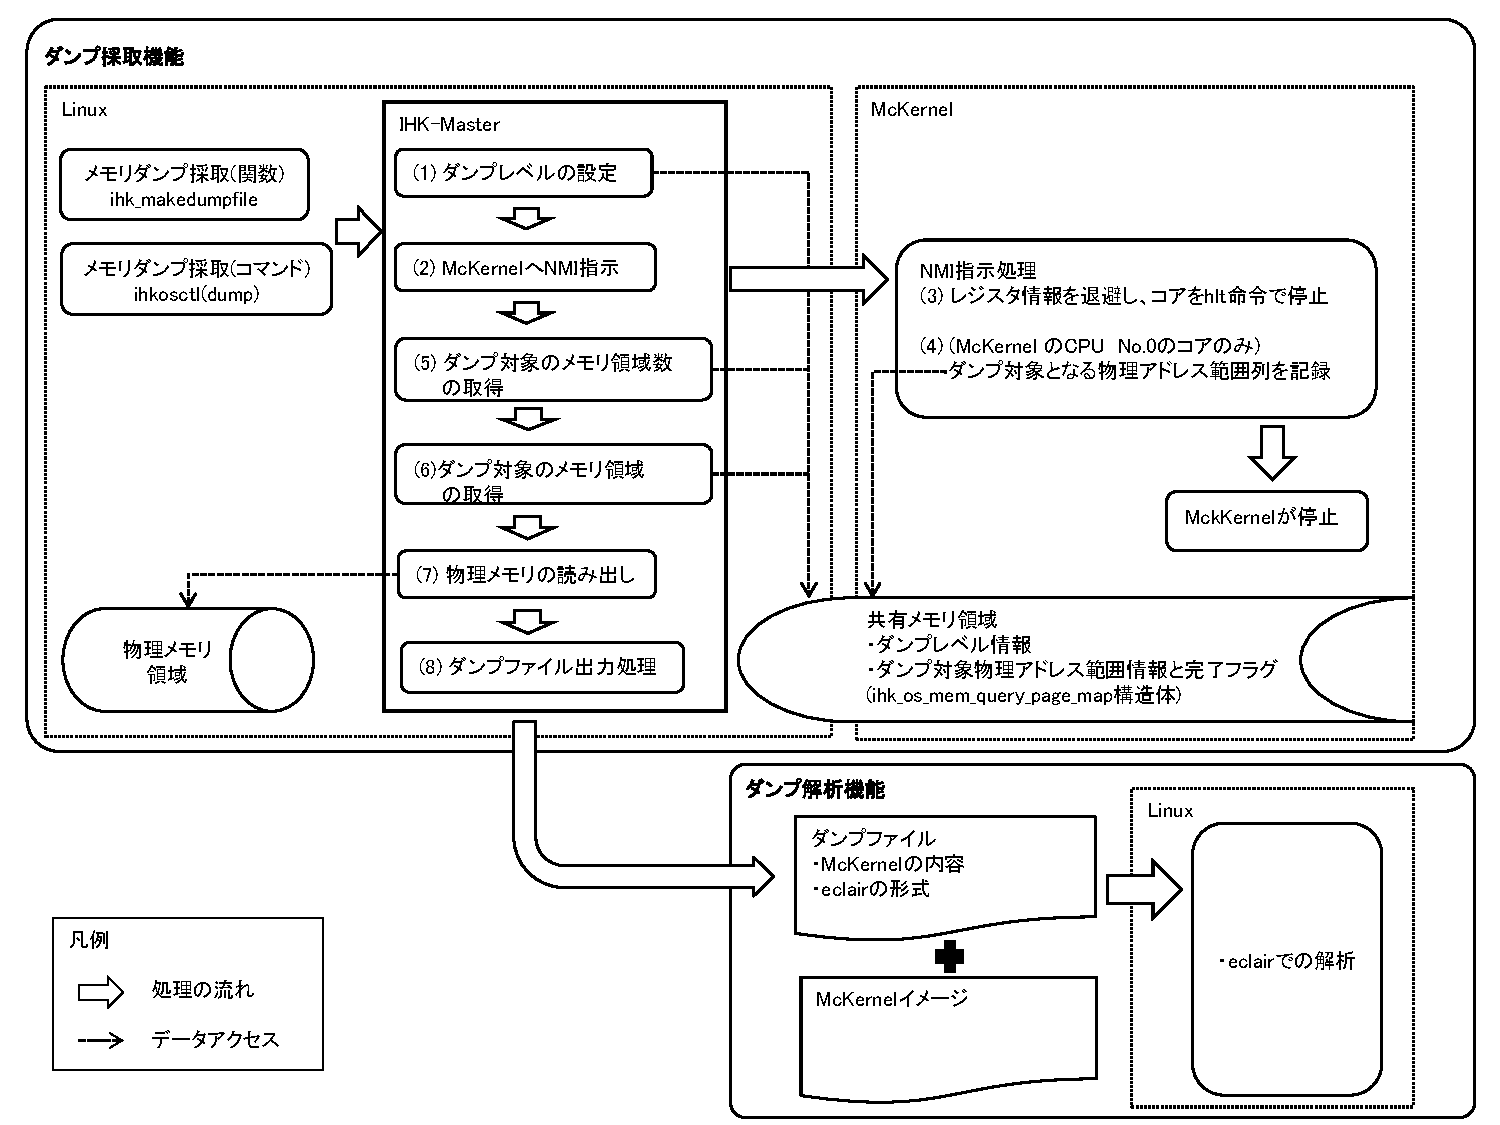
\includegraphics[scale=0.6]{figs/chap01_fig006.pdf}
  \caption{McKernel主導ダンプの場合のダンプ採取機能とダンプ形式変換機能の処理の流れ}
  \label{figure:chap01_fig006}
\end{figure} 
\FloatBarrier
%
\begin{enumerate}
\item IHKがOSブート時に、各物理ページがダンプ対象であるかを示す情報(以下、ダンプ対象ページリストと呼ぶ)をLinuxとMcKernelとで共有しているメモリ領域(以降、共有メモリと呼ぶ)に確保する。また、IHKがMcKernelに割り当てた物理アドレス範囲をダンプ対象とするように初期化する。
\item 管理者が\texttt{ihk\_os\_makedumpfile()}でダンプを指示する。
\item IHKが共有メモリにダンプレベルを記録する。また、共有メモリ上の、ダンプ対象ページリストの設定完了を表すフラグ(以降、完了フラグと呼ぶ)を0に設定する。 (図の(1))
\item IHKがMcKernelの各コアへNMIを送る。(図の(2))
\item McKernelの第0~CPU以外のCPUはレジスタ情報を退避した後\texttt{hlt}命令で停止する(図の(3)) 。 McKernelの第0~CPUは以下を実行する。(図の(3)、(4)) 
\begin{enumerate}
\item レジスタ情報を退避する。
\item 共有メモリを参照してダンプレベルを取得する。
\item ダンプからユーザ領域を除外する指定がされている場合は、ユーザメモリ領域情報を取得し、ダンプ対象ページリストの対応ビットを0にする。
\item ダンプから未使用領域を除外する指定がされている場合は、未使用メモリ領域情報を取得し、ダンプ対象ページリストの対応ビットを0にする。
\item 完了フラグに1をセットする。
\item \texttt{hlt}命令で停止する。
\end{enumerate}
\item IHKが完了フラグが1になるまで待ち、\texttt{ioctl()}でダンプ対象のメモリ領域数を取得し、領域情報を格納するメモリ領域を確保し、さらに\texttt{ioctl()}でダンプ対象の領域情報を前記メモリ領域に記録する。(図の(5)、(6))
\item IHKがダンプ対象のメモリ領域を\texttt{ioctl()}で読み出し、ファイルに書き込む。(図の(7)、(8))
\item 管理者はeclairを用いてダンプファイルの解析を行う。
\end{enumerate}

ダンプ対象は\texttt{ihk\_dump\_page\_set}で表現する。定義は以下の通り。
\begin{verbatim}
struct ihk_dump_page_set {
    unsigned int completion_flag;  /* 書き込み完了フラグ */
    unsigned int count;            /* ダンプ対象のページ情報数 */
    unsigned long page_size;       /* ダンプ対象のページ情報の全体サイズ */
    unsigned long phy_page;        /* ダンプ対象のページ情報の物理アドレス
                                      (struct ihk_dump_pageの配列) */
}

struct ihk_dump_page {
    unsigned long start;       /* マップ情報の開始物理アドレス */
    unsigned long map_count;   /* マップ情報の領域数(map[]の配列数) */
    unsigned long map[];       /* マップ情報(ビットマップ形式) */
};
\end{verbatim}


Linux主導ダンプの場合のダンプ採取機能とダンプ形式変換機能の処理の流れを図\ref{figure:chap01_fig007}を用いて説明する。
\begin{figure}[!ht]
  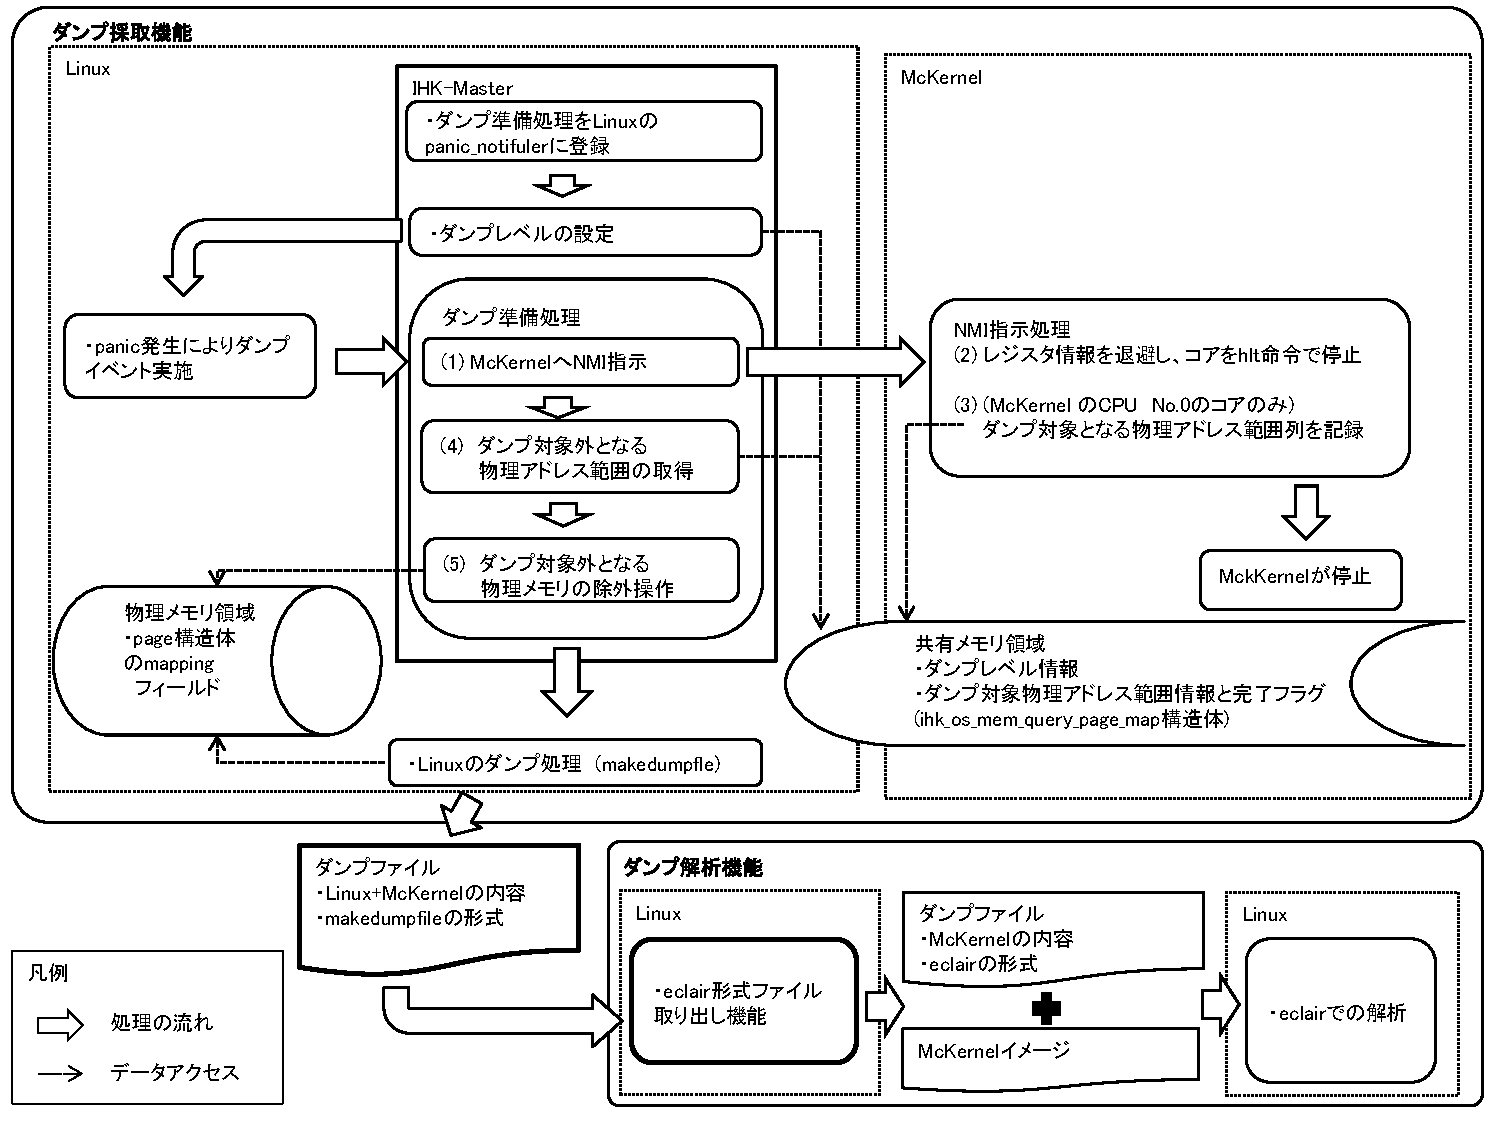
\includegraphics[scale=0.6]{figs/chap01_fig007.pdf}
  \caption{Linux主導ダンプの場合のダンプ採取機能とダンプ形式変換機能の処理の流れ}
  \label{figure:chap01_fig007}
\end{figure}
\FloatBarrier
%
\begin{enumerate}
\item IHKがOSブート時に、ダンプ対象ページリストを共有メモリに確保する。また、IHKがMcKernelに割り当てた物理アドレス範囲をダンプ対象とするように初期化する。
\item IHKがMcKernel起動時にダンプレベル設定オプション(-d)でダンプレベルを指定する。IHKは共有メモリにこのダンプレベルを記録する。また、完了フラグを0に設定する。
\item IHKがダンプ準備処理関数をLinuxの\texttt{panic\_notifier}に登録する。
\item Linuxでpanicが発生し、登録されているダンプ準備処理関数が呼び出される。
\item IHKがMcKernelの各コアへNMIを送る。(図の(1))
\item McKernelの第0~CPU以外のCPUは、レジスタ情報を退避し、\texttt{hlt}命令で停止する(図の(3))。McKernelの第0~CPUは以下を実行する。(図の(2)、(3)))
\begin{enumerate}
\item レジスタ情報を退避する。
\item 共有メモリを参照してダンプレベルを取得する。
\item ダンプからユーザ領域を除外する指定がされている場合は、ユーザメモリ領域情報を取得し、ダンプ対象ページリストにダンプからの除外を記録する。
\item ダンプから未使用領域を除外する指定がされている場合は、未使用メモリ領域情報を取得し、ダンプ対象ページリストのダンプからの除外を記録する。
\item 完了フラグに1をセットする。
\item \texttt{hlt}命令で停止する。
\end{enumerate}
\item IHKが完了フラグが1になるまで待ち、\texttt{ioctl()}でダンプ対象外の物理アドレス範囲に該当するLinuxのpage構造体の\texttt{mapping}フィールドを操作しanonymousに設定する。(図の(4)、(5)))
\item Linuxが\texttt{makedumpfile}コマンドを実行する。
\item LinuxがLinuxとMcKernelの両方の情報を含むダンプファイルを作成する。
\item 管理者が\texttt{ldump2mcdump}コマンドで、\texttt{makedumpfile}形式のダンプファイルをeclair形式に変換する。
\item 管理者はeclairを用いてダンプファイルの解析を行う。
\end{enumerate}



\subsection{\MODAUGS{ユーザメモリ領域情報取得}}
\begin{figure}[!ht]
  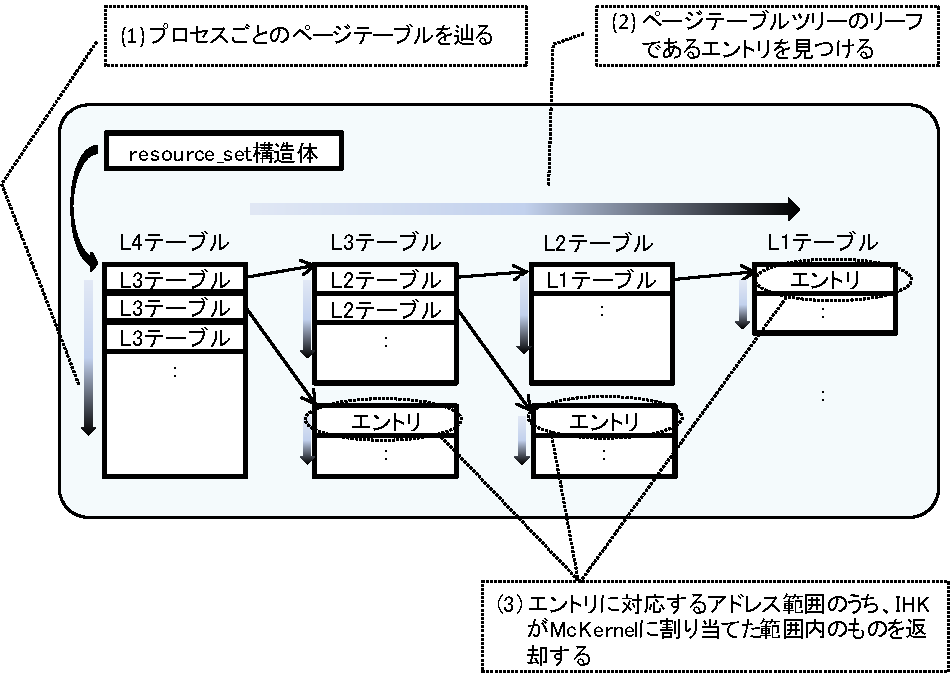
\includegraphics[width=0.9\linewidth]{figs/chap01_fig009.pdf}
  \caption{ユーザメモリ領域情報取得処理の流れ}
  \label{figure:chap01_fig009}
\end{figure}
\FloatBarrier
%
ユーザメモリ領域情報取得処理の流れを図\ref{figure:chap01_fig009}を用いて説明する。
\begin{enumerate}
\item \texttt{resource\_set}を参照して全プロセスを辿り、プロセスごとのページテーブルについて以下を行う。(図の(1))
\begin{enumerate}
\item ページテーブルツリーのリーフであるエントリを見つける。(図の(2))なお、4段目のエントリは4~KBページのエントリ、3段目かつPageSizeフラグが1のエントリは2~MB、2段めかつPageSizeフラグが1のエントリは1~GBページのエントリである。
\item エントリに対応するアドレス範囲のうち、IHKがMcKernelに割り当てた範囲に収まるものをユーザメモリ領域として返却する。収まらないものはエントリが破壊されているとみなし破棄する。(図の(3))
\end{enumerate}
\comment{
\item 当該物理アドレス範囲に対応するダンプ対象ページリスト(\texttt{ihk\_os\_mem\_query\_page\_map}構造体)のビットを以下の手順で0にし、ダンプ対象からの除外を記録する。
\begin{enumerate}
\item ダンプ対象ページリストの配列インデックスを以下の計算式で算出する。\\
(当該物理アドレス\UTF{FF0D}McKernelに割り当てられた物理メモリの開始アドレス)の値を18ビット右シフトした値
\item ダンプ対象ページリストのビット位置を以下の計算式で算出する。 \\
(当該物理アドレス\UTF{FF0D}McKernelに割り当てられた物理メモリの開始アドレス)の値を12ビット右シフトした値の下位6ビットの値
\item 上記ビット位置から(ページサイズ / 4096)個のビットを0にする。
\end{enumerate}
}
\end{enumerate}

\subsection{\MODAUGS{未使用メモリ領域情報取得}}

\begin{figure}[!ht]
  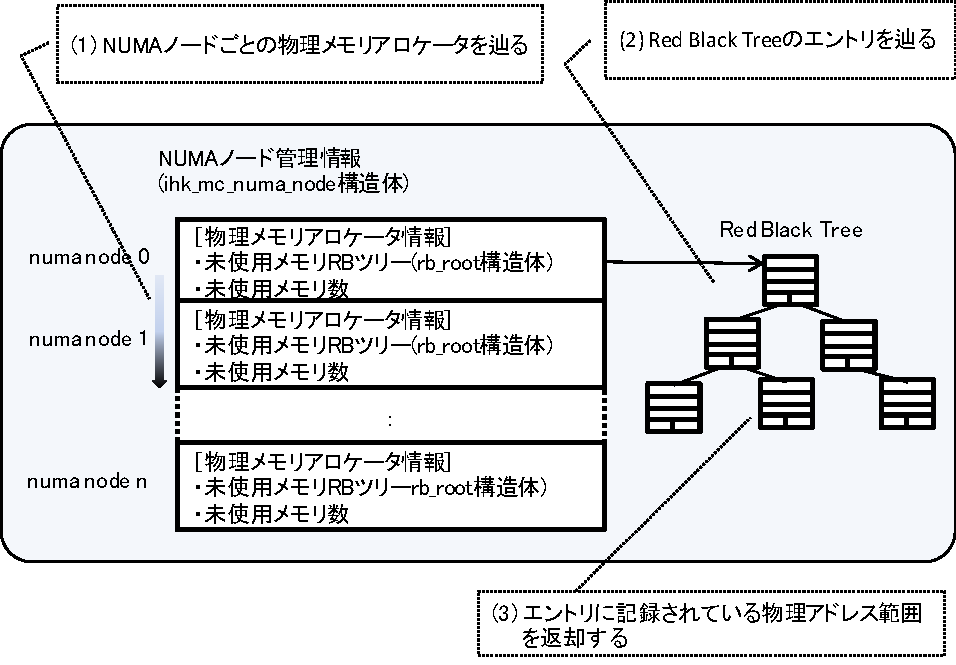
\includegraphics[width=0.9\linewidth]{figs/chap01_fig010.pdf}
  \caption{未使用メモリ領域情報取得処理の流れ}
  \label{figure:chap01_fig010}
\end{figure}
\FloatBarrier
%
未使用メモリ領域情報取得の処理の流れを図\ref{figure:chap01_fig010}を用いて説明する。
\begin{enumerate}
\item NUMAノード管理情報(\texttt{ihk\_mc\_numa\_node}構造体)を参照してNUMAノードごとの物理メモリアロケータについて以下を行う。(図の(1))
\begin{enumerate}
\item 未使用メモリを管理するRed Black tree(rb\_root構造体)のエントリを辿る。(図の(2))
\item エントリ(\texttt{free\_chunk}構造体)に記録されている物理アドレス範囲を返却する。(図の(3))
\end{enumerate}
\comment{
\item 当該物理アドレス範囲に対応するダンプ対象ページリスト(\texttt{ihk\_os\_mem\_query\_page\_map}構造体)にダンプ対象からの除外を記録する。
\begin{enumerate}
\item ダンプ対象ページリストの配列インデックスを以下の計算式で算出する。\\
(当該物理アドレス\UTF{FF0D}McKernelに割り当てられた物理メモリの開始アドレス)の値を18ビット右シフトした値
\item ダンプ対象ページリストのビット位置を以下の計算式で算出する。 \\
(当該物理アドレス\UTF{FF0D}McKernelに割り当てられた物理メモリの開始アドレス)の値を12ビット右シフトした値の下位6ビットの値
\item 上記ビット一から(サイズ / 4096)個のビットを0にする。
\end{enumerate}
}
\end{enumerate}

\comment{
\subsection{McKernel主導ダンプでのダンプ対象メモリ領域取得}\label{sec:mckernel_memory_exclusion}

McKernel主導ダンプでのダンプ対象メモリ領域取得の処理の流れを図\ref{figure:chap01_fig011}を用いて説明する。
\begin{figure}[!ht]
  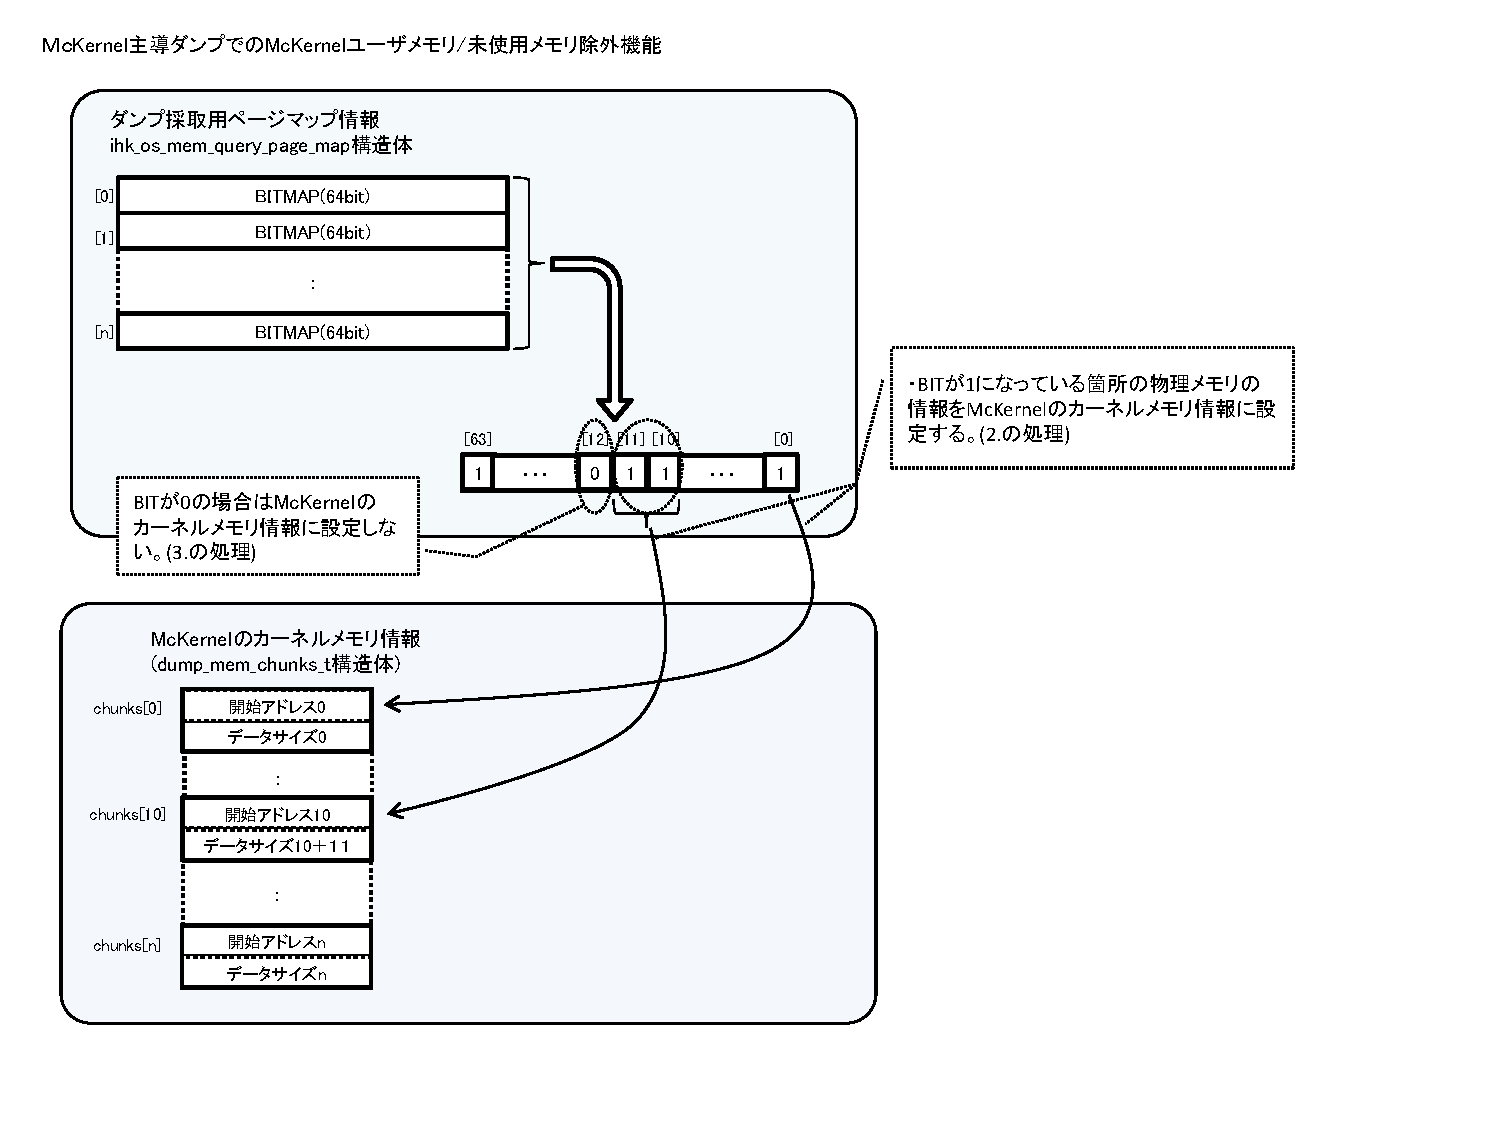
\includegraphics[scale=0.6]{figs/chap01_fig011.pdf}
  \caption{ダンプ対象メモリ領域取得処理の流れ}
  \label{figure:chap01_fig011}
\end{figure}
\FloatBarrier
%
\begin{enumerate}
\item ダンプ対象ページリスト(ihk\_os\_mem\_query\_page\_map構造体)を参照し、2\UTF{FF5E}3の処理を行う。
\item ビットマップ情報のビットが1になっている箇所の物理メモリの開始アドレスとサイズを算出し、McKernelのカーネルメモリ情報(dump\_mem\_chunks\_t構造体)
に設定する。
※ビットが連続で1になっている箇所は連続しているビット数分のデータサイズで算出する。\newline\newline
以下で手順で開始アドレスを算出する。
\begin{enumerate}
\item[(1)] McKernelに割り当てられた物理メモリの開始アドレスからの相対アドレス値を算出する。 \newline
計算式:ダンプ対象ページリストのmap配列のindex値を18ビット左シフトした値+ダンプ対象ページリストのビット位置の値を12ビット左シフトした値
\item[(2)] ダンプ対象のカーネルメモリ情報の開始アドレスを算出する。 \newline
計算式:McKernelに割り当てられた物理メモリの開始アドレス+(1)で算出した相対アドレス値
\end{enumerate}
データサイズはON(1)になっているビット数を12ビット左シフトし算出する。\newline
\item ビットマップ情報のビットが0になっている箇所は除外対象なので、McKernelのカーネルメモリ情報(dump\_mem\_chunks\_t構造体)に保持しない。
\end{enumerate}

\subsection{Linux主導ダンプでのMcKernelユーザメモリ/未使用メモリ除外機能}\label{sec:mckernel_memory_exclusion}

Linux主導ダンプでのMcKernelユーザメモリ/未使用メモリ除外機能の処理を図\ref{figure:chap01_fig012}で示す。\newline
\begin{figure}[!ht]
  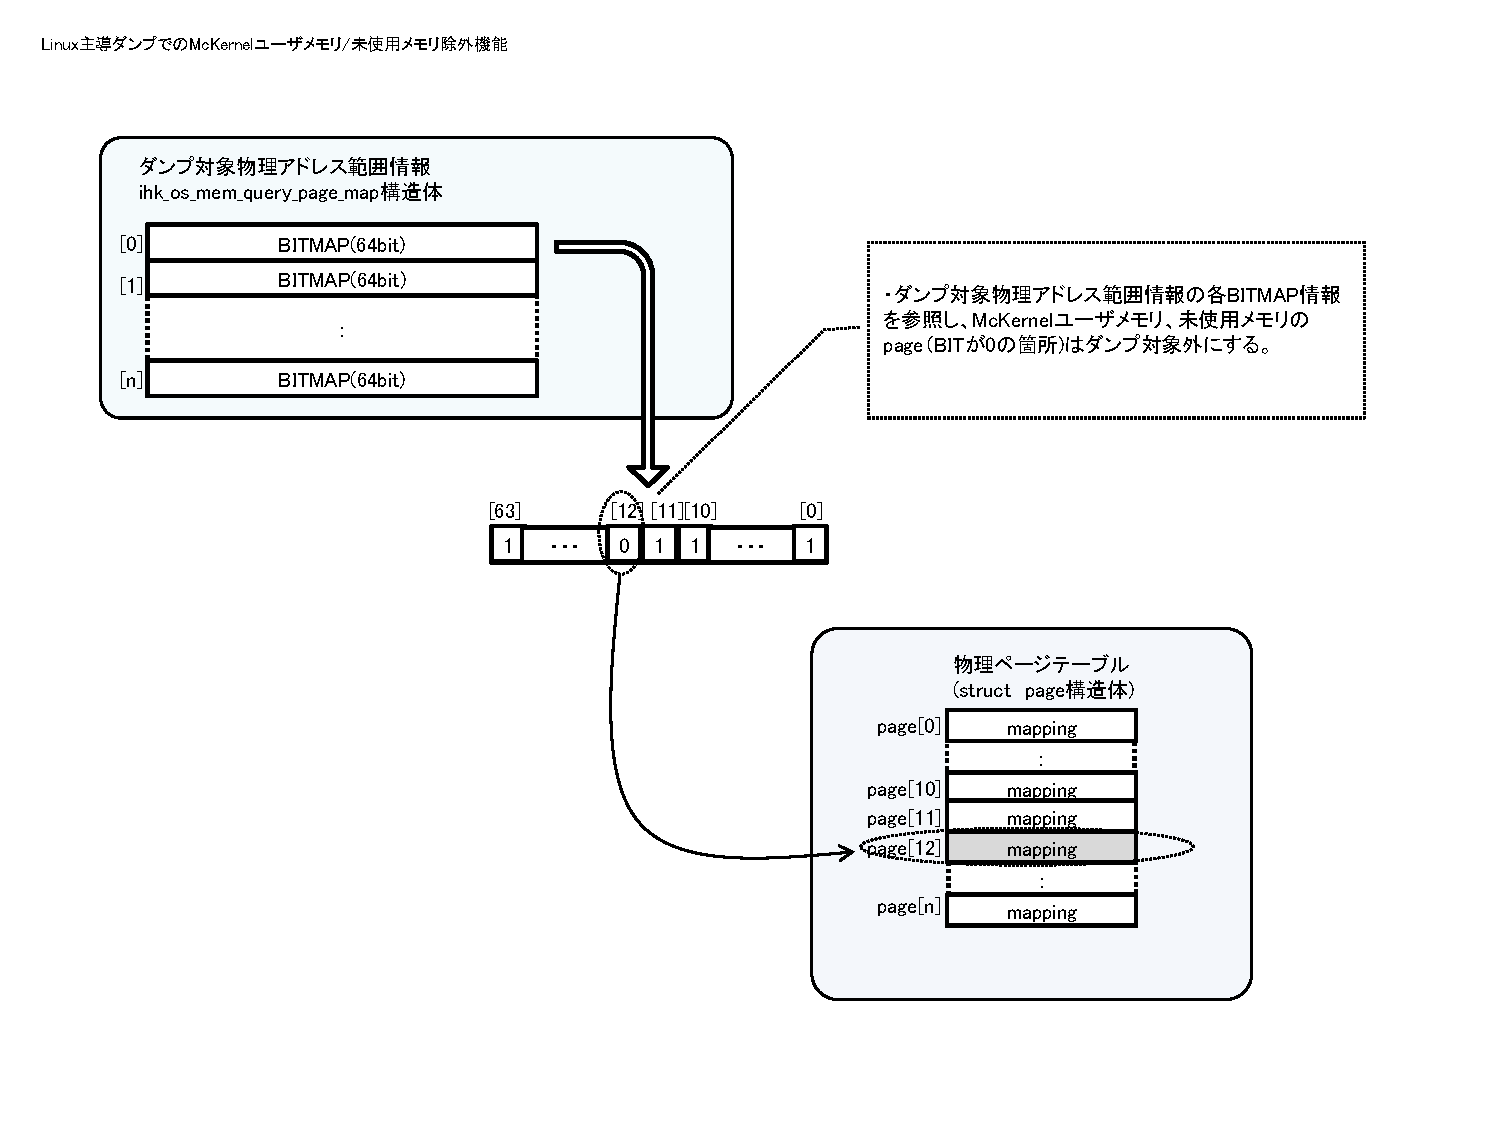
\includegraphics[scale=0.6]{figs/chap01_fig012.pdf}
  \caption{Linux主導ダンプでのMcKernelユーザメモリ/未使用メモリ除外機能}
  \label{figure:chap01_fig012}
\end{figure}
\FloatBarrier

Linux主導ダンプでのMcKernelユーザメモリ、未使用メモリ除外機能として、ダンプ対象ページリスト(ihk\_os\_mem\_query\_page\_map構造体)を参照し、全情報分、以下の処理を繰り返す。\newline
\begin{enumerate}
\item ダンプ対象ページリストのビットマップ情報のビットが0になっている箇所を見つける。
\item ビットが0になっている箇所に該当する物理ページテーブルのページ番号を算出する。\newline
計算式:ダンプ採取用ページマップ情報のmap配列のindex値を6ビット左シフトした値+ダンプ採取用ページマップ情報のビット位置の値
\item 物理ページテーブルの該当pageのmappingフィールドデータの最下位ビットに1を設定し、anonymousであることを記録する。\newline
\end{enumerate}
}


\comment{
\subsubsection{\texttt{do\_dump}関数のラッピング処理}
\subsubsection*{書式}{\quad} \texttt{int ihk\_makedumpfile(int index, char *dump\_file, int dump\_level);}
\subsubsection*{説明}{\quad} 
ダンプファイル名とダンプレベルをdo\_dump()の引数に設定する。
\begin{enumerate}
\item do\_dump()を呼び出す。
\item do\_dump()の結果を戻り値に設定する。
\end{enumerate}

\subsubsection*{戻り値}{\quad}
\begin{itemize}
\item       0 :正常終了
\item --ENOENT :dump\_fileの値がNULL、またはdump\_fileが長さ0の文字列を指している、またはdump\_fileに含まれるディレクトリが存在しない。
\item --EACCESS:dump\_fileで指定したファイルについて、ディレクトリは存在するがファイルが作成できない。
\item --EEXIST :dump\_fileの値がNULL、またはdump\_fileが長さ0の文字列を指している、またはdump\_fileに含まれるディレクトリが存在しない。
\item --EINVAL :不正なパラメタ。indexが負の場合を含む。
\item --ENODEV :indexで指定されるOSインスタンスが存在しない。
\item --EPERM  :indexで指定されるOSインスタンスにアクセスできない
\end{itemize}
}

\ifx \HLDIFFJULTWO y
\subsection{\RMJULTWOS{Linux主導ダンプでの除外領域設定}}
\subsubsection*{書式}{\quad} \texttt{int ihk\_linux\_initiated\_dump\_set\_level(int index, int dump\_level)}
\subsubsection*{説明}{\quad} 
\begin{enumerate}
\item indexが負の場合を含む。不正なパラメータの場合は--EINVAL を返却する。
\item indexで指定されるOSインスタンスが存在しない場合は--ENODEVを返却する。
\item indexで指定されるOSインスタンスにアクセスできない場合は--EPERMを返却する。
\item OS番号、ダンプレベルを設定し、ioctl(fd, IHK\_OS\_LINUX\_INITIATED\_DUMP\newline \_SET\_LEVEL,dump\_level)を呼び出す。
\item OS番号を設定し、ioctl(fd, IHK\_OS\_LINUX\_INITIATED\_DUMP\_UNMARK)を呼び出す。
\item0を返却する。
\end{enumerate}

\subsubsection*{戻り値}{\quad}
\begin{itemize}
\item 0      :正常終了
\item --EINVAL:不正なパラメタ。indexが負の場合を含む。
\item --ENODEV:indexで指定されるOSインスタンスが存在しない
\item --EPERM :indexで指定されるOSインスタンスにアクセスできない。
\end{itemize}
\fi

\ifx \HLDIFFJULTWO y
\subsection{\RMJULTWOS{ダンプ処理}}
\subsubsection*{書式}{\quad} \texttt{int do\_dump(int osfd, int dump\_level, char *dump\_file)}
\subsubsection*{説明}{\quad} 

do\_dumpはダンプ採取関数 (ihk\_makedumpfile)及びダンプ採取コマンド(ihkosctl dump)により呼びだされる。
\begin{enumerate}
\item dump\_fileの値がdump\_fileの値がNULL、またはdump\_fileが長さ0の文字列を指している、またはdump\_fileに含まれるディレクトリが存在しない場合は、--ENOENTを返却する。
\item dump\_fileで指定したファイルについて、ディレクトリは存在するがファイルが作成できない場合は--EACCESSを返却する。
\item dump\_fileの値がNULL、またはdump\_fileが長さ0の文字列を指している、またはdump\_fileに含まれるディレクトリが存在しない場合は--EEXISTを返却する。
\item indexが負の場合を含む。不正なパラメータの場合は--EINVAL を返却する。
\item indexで指定されるOSインスタンスが存在しない場合は--ENODEVを返却する。
\item indexで指定されるOSインスタンスにアクセスできない場合は--EPERMを返却する。
\item 物理メモリ領域情報取得用のメモリ領域を確保する。
\item システム時間、ホスト名を取得する。
\item ioctl(osfd, IHK\_OS\_DUMP, \&args)[args.cmd=DUMP\_SET\_LEVEL]を呼び出す。
\item ioctl(osfd, IHK\_OS\_DUMP, \&args)[args.cmd = DUMP\_NMI]を呼び出す。
\item ioctl(osfd, IHK\_OS\_DUMP, \&args)[args.cmd=DUMP\_QUERY\_NUM\_MEM\_AREAS]を呼び出す。
\item 取得したIHKによって割り当てられた物理メモリ領域情報のサイズを算出する。
\item ioctl(osfd, IHK\_OS\_DUMP, \&args)[args.cmd=DUMP\_QUERY\_MEM\_AREAS]を呼び出す。
\item ファイル出力用のバッファのメモリ領域を確保する。
\item システム日付を取得する。
\item dump\_file名が設定されていた場合、"dump\_file名\_YYYYmmddHHMMSS"の形式でファイル名を設定する。
\item 取得した物理メモリ領域情報をダンプファイルに出力する。
\end{enumerate}

\subsubsection*{戻り値}{\quad}
\begin{itemize}
\item       0 :正常終了
\item --ENOENT :dump\_fileの値がNULL、またはdump\_fileが長さ0の文字列を指している、またはdump\_fileに含まれるディレクトリが存在しない。
\item --EACCESS:dump\_fileで指定したファイルについて、ディレクトリは存在するがファイルが作成できない。
\item --EEXIST :dump\_fileの値がNULL、またはdump\_fileが長さ0の文字列を指している、またはdump\_fileに含まれるディレクトリが存在しない。
\item --EINVAL :不正なパラメタ。indexが負の場合を含む。
\item --ENODEV :indexで指定されるOSインスタンスが存在しない。
\item --EPERM  :indexで指定されるOSインスタンスにアクセスできない。
\end{itemize}
\fi

\subsection{\MODJULTWOS{ダンプ処理用ioctl()コマンド}}

\subsubsection*{書式}{\quad} \texttt{int ioctl(int fd, IHK\_OS\_DUMP, struct ihk\_dump\_args *args)}
\subsubsection*{説明}{\quad} 
\texttt{fd}で指定されたOSインスタンスに対して、\texttt{args->cmd}に指定されたダンプ関連処理を行う。

%\subsubsection*{書式}{\quad} \texttt{int smp\_ihk\_os\_dump(ihk\_os\_t ihk\_os, void *priv, dumpargs\_t *args)}
%\subsubsection*{説明}{\quad} 

\texttt{dumpargs\_t}は以下のように定義される。
\begin{verbatim}
struct ihk_dump_args {
    int cmd;                    /* コマンド */
    unsigned int level;         /* ダンプレベル */
    long start;                 /* 開始物理アドレス */
    long size;                  /* サイズ */
    void *buf;                  /* メモリ内容 */
    int num_mem_chunks;         /* メモリ領域数 */
    struct ihk_dump_mem_chunk *mem_chunks; /* メモリ領域情報 */
};
\end{verbatim}

\texttt{struct ihk\_dump\_mem\_chunk}は以下のように定義される。
\begin{verbatim}
struct ihk_dump_mem_chunk {
    unsigned long addr;
    unsigned long size;
};
\end{verbatim}

\texttt{args->cmd}ごとの処理は以下の通り。

\begin{table}[!h]
\footnotesize
\begin{tabular}{|p{0.28\linewidth}|p{0.67\linewidth}|} \hline
\multicolumn{1}{|c}{\textbf{\texttt{args->cmd}}}&\multicolumn{1}{|c|}{\textbf{動作}}\\ \hline \hline
\textttw{DUMP\_QUERY\_NUM\_MEM\_AREAS}&ダンプ対象メモリ領域数を返す。\\ \hline
\texttt{DUMP\_QUERY\_MEM\_AREAS}&ダンプ対象メモリ領域の情報を\texttt{args->mem\_chunks}に格納する。呼び出し元が\texttt{args->mem\_chunks}の領域を用意する。\\ \hline
\texttt{DUMP\_READ}&\texttt{args->start, args->size}で指定された物理メモリ領域の内容を\texttt{args->buf}で指定されたバッファにコピーする。\\ \hline
\texttt{DUMP\_SET\_LEVEL}&\begin{tabular}[t]{@{}l@{}}
ダンプ対象とするメモリ領域の種類を\texttt{args->level}に設定する。設定可能\\
な値は以下の通り。\\
  \begin{tabular}[t]{|p{0.05\linewidth}|p{0.85\linewidth}|} \hline
    0&IHKがMcKernelに割り当てたメモリ領域を出力する。\\ \hline
    24&カーネルが使用しているメモリ領域を出力する。\\ \hline
  \end{tabular}\vspace{0.5em}\\
なお、\texttt{args->level}が設定可能でない値であった場合は\texttt{-EINVAL}を返却\\
する。
\end{tabular}
\\ \hline
\texttt{DUMP\_NMI}&全CPUにNMIを発行し、ダンプの準備を指示する。\\ \hline
\texttt{DUMP\_SET\_ANONYMOUS}&(IHKがMcKernelに割り当てたメモリ領域)から(\texttt{args->mem\_chunks, args->num\_mem\_chunks}で指定したメモリ領域)を除いた領域に対し、Linuxの\texttt{struct page}の\texttt{mapping}フィールドの最下位ビットをセットしanonymousテーブルに見せかける。こうすることで、Linuxの\texttt{makedumpfile}が該当領域をダンプ対象から除外できるようになる。\\ \hline
\texttt{DUMP\_QUERY}&IHKによって割り当てられた物理メモリ領域の情報を\texttt{args->start, args->size}に格納する。本機能は、IHKがMcKernelに割り当てたメモリ領域の全てをダンプする際に使用する。\\ \hline
\end{tabular}
\vspace{-0em}
\end{table}
\FloatBarrier

\comment{
\texttt{IHK\_OS\_LINUX\_INITIATED\_DUMP\_SET\_LEVEL}
Linux主導ダンプにおいてダンプから除外する領域をdump\_levelで指定する。\newline
dump\_levelは除外するメモリ領域のタイプを整数で指定する。\newline
dump\_levelは設定可能な整数かどうかのチェックを行い、不正な場合は--EINVAL(不正なパラメタ)を返却する。
\begin{itemize}
\item  0:除外せずにMcKernelに割り当てられたメモリ領域の全てのページを出力する。
\item 24:ユーザページと未使用ページを除外する。
\end{itemize}
}
\comment{
\texttt{IHK\_OS\_LINUX\_INITIATED\_DUMP\_UNMARK}
Linux主導ダンプにおいて、指定されたメモリ領域が除外されるようにLinux側での操作を行う。除外対象はLinux主導ダンプのダンプレベル設定のioctl()で設定される。
}


\subsubsection*{戻り値}
\begin{table}[!h]
\footnotesize
\begin{tabular}{|p{0.20\linewidth}|p{0.75\linewidth}|} \hline
0&正常終了\\ \hline
\texttt{-EFAULT}&アドレスが不正である\\ \hline
\texttt{-EINVAL}&引数が無効である\\ \hline
\end{tabular}
\vspace{-0em}
\end{table}
\FloatBarrier

\subsubsection{ダンプファイルの形式}	
ダンプファイルはELF形式を採用している。ダンプファイルで使用しているセクションは以下の通り。
\begin{table}[!h]
\footnotesize
\begin{tabular}{|p{0.20\linewidth}|p{0.75\linewidth}|} \hline
\multicolumn{1}{|c}{\textbf{セクション名}}&\multicolumn{1}{|c}{\textbf{説明}}\\ \hline \hline
\texttt{Date}&\begin{tabular}[t]{@{}l@{}}ダンプ採取日時\\例: \texttt{Thu Mar  3 21:42:35 2016}\end{tabular}\\ \hline
\texttt{hostname}&\begin{tabular}[t]{@{}l@{}}ダンプ採取ホスト名\\例: \texttt{kncc08}\end{tabular}\\ \hline
\texttt{User}&\begin{tabular}[t]{@{}l@{}}ダンプ採取 実ユーザ名\\例: \texttt{nakamura}\end{tabular}\\ \hline
\texttt{physmem}&物理メモリダンプ\\ \hline
\end{tabular}
\vspace{-0em}
\end{table}
\FloatBarrier

なお、レジスタの値はダンプファイルには格納しない。その代わり、スレッドを表現する構造体に格納されている退避コンテキストから値を取得する。スレッドを表現する構造体の位置は、まず各コアのrun queueの位置をシンボル情報から取得し、そこに挿入されているエントリを見つけることで取得する。
\texttt{objdump}での出力例を図\ref{figure:chap01_fig008}に示す。
%
\begin{figure}[!ht]
  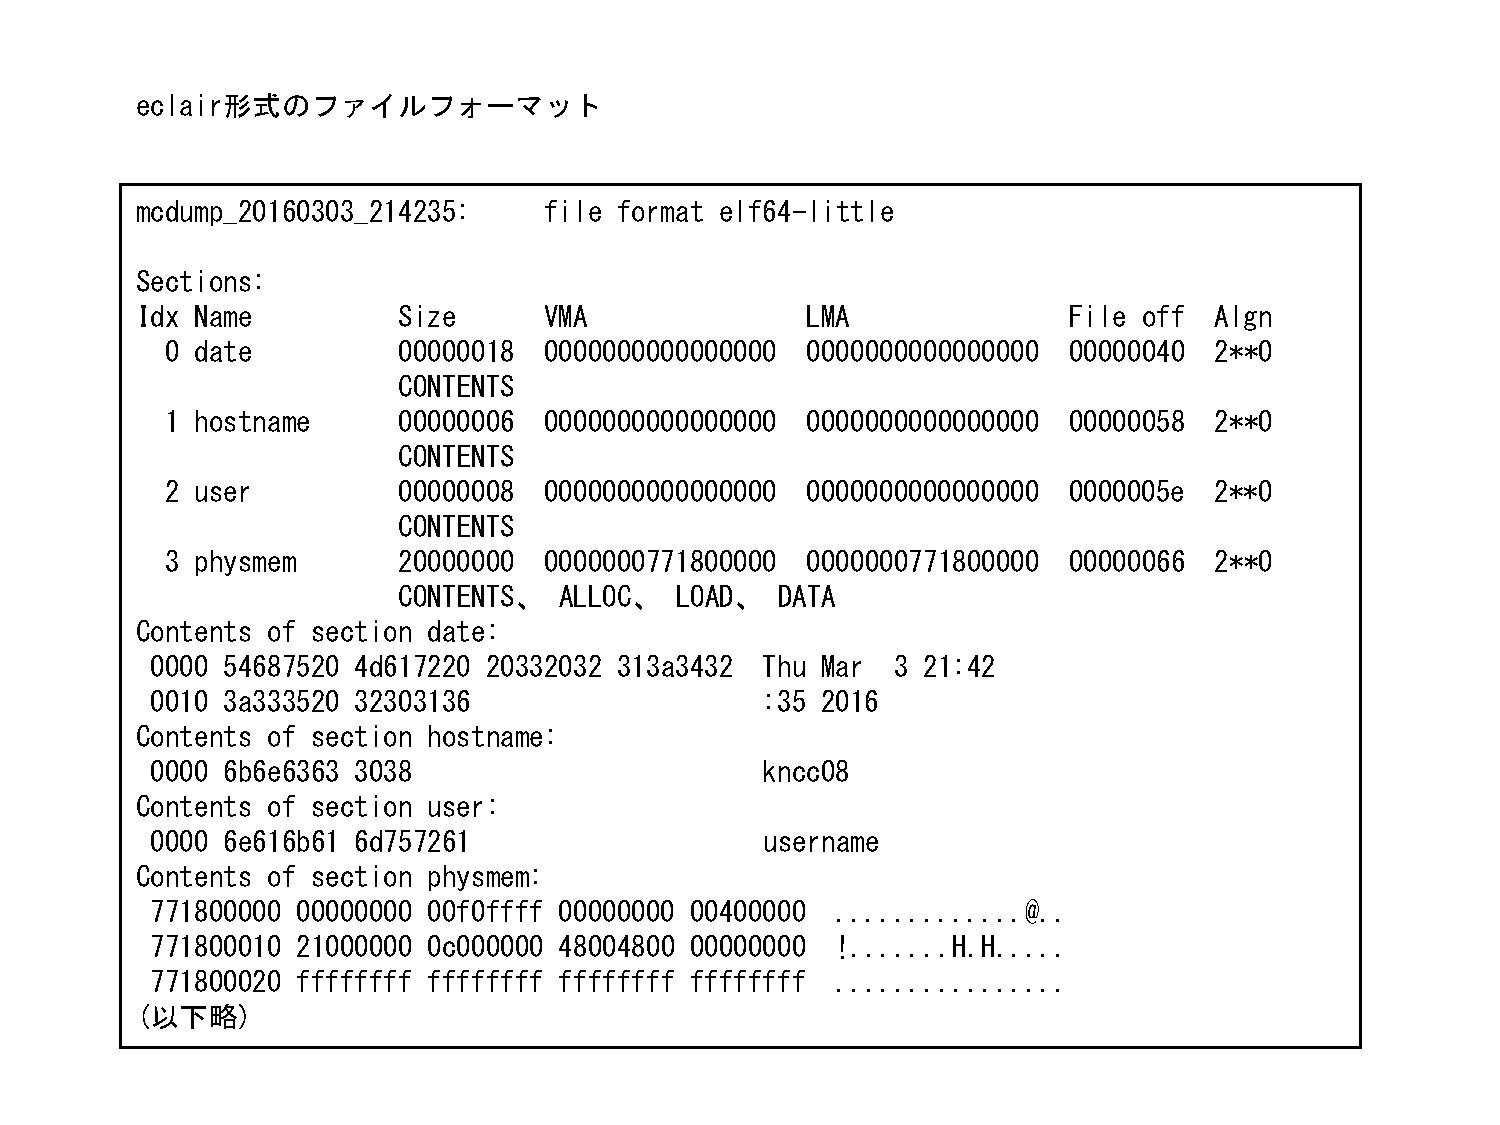
\includegraphics[scale=0.6]{figs/chap01_fig008.pdf}
  \caption{ダンプファイルの\texttt{objdump}での出力例}
  \label{figure:chap01_fig008}
\end{figure}
\FloatBarrier

\subsection{ダンプ解析コマンドとgdbコマンドとの連携方法}
ダンプ解析コマンドとgdbコマンドとの間のremote serial protocolは、IPv4を使ったTCP通信でやり取りする。unixドメインソケットなども利用可能とは思うが、異常終了時にごみファイルが残ることを回避するためにTCP/IP通信を選択した。
ユーザが直接gdbを起動して毎回リモートデバッグの設定を行うことは、難しくはないが面倒である。そこで、ユーザには、gdbではなくダンプ解析コマンドを起動してもらう。ダンプ解析コマンドがgdbコマンドの起動とリモートデバッグの設定を行う。
ダンプ解析コマンドによるリモートデバッグの設定から、実際にユーザからの解析コマンドを受け取るgdbに、スムーズに端末を受け渡すため、以下の手順で動作する。
\begin{enumerate}
\item ユーザから起動されたダンプ解析コマンドは、コマンドラインオプションを解析してgdbエージェントとしての初期化をする。
\item ダンプ解析コマンドは、remote serial protocol通信用のTCPソケットを作成する。
\item ダンプ解析コマンドは、gdbをfork()とexec()で起動する。この時、以下のようなコマンドライン引数としてリモートデバッグの設定に必要なコマンドを与える。\\
\footnotesize
\begin{verbatim}
-q -ex set prompt (eclair) -ex target remote :<TCPポート番号> <カーネルイメージファイル名>
\end{verbatim}
\normalsize
\item ダンプ解析コマンドは、TCPソケットにgdbが接続してくるのを待つ。
\item ダンプ解析コマンドは、TCPソケット接続後、端末からの入力をせずにgdbエージェントとしての動作に専念する。
\end{enumerate}
上記の手順によって、ダンプ解析コマンドとgdbとが同じ端末を共有した状態になる。共有していても、標準入力の読み出しをダンプ解析コマンドが一切実行しなければ、gdbが標準入力を占有しているのと同じ動作をさせることができる。

\ifx \HLDIFFJULTWO y
\subsection{\RMJULTWOS{eclair形式ファイル取り出し}}
\subsubsection*{書式}{\quad} \texttt{void ldump2mcdump(int osfd, char *dump\_file)}
\subsubsection*{説明}{\quad} 
makedumpfile形式のダンプファイルをMcKernel形式に変換し、\texttt{dump\_file}と\textttw{\_YYYYmmddHHMMSS}をつなぎ合わせた名前のファイルに出力する。

動作ステップは以下の通り。
\begin{enumerate}
\item \texttt{ihk.ko, ihk-smp-x86.ko, mcctrl.ko}が記録している、IHKがMcKernelに割り当てた物理メモリ領域の情報をシンボル情報を用いて取得する。
\item 上記物理メモリ領域を用いてダンプファイルからMckernel関連の情報を取得し、eclair形式に変換してファイルに出力する。
\end {enumerate}
\fi

\subsection{\MODAUGS{ダンプ形式変換(crashプラグイン)}}
\begin{figure}[!ht]
  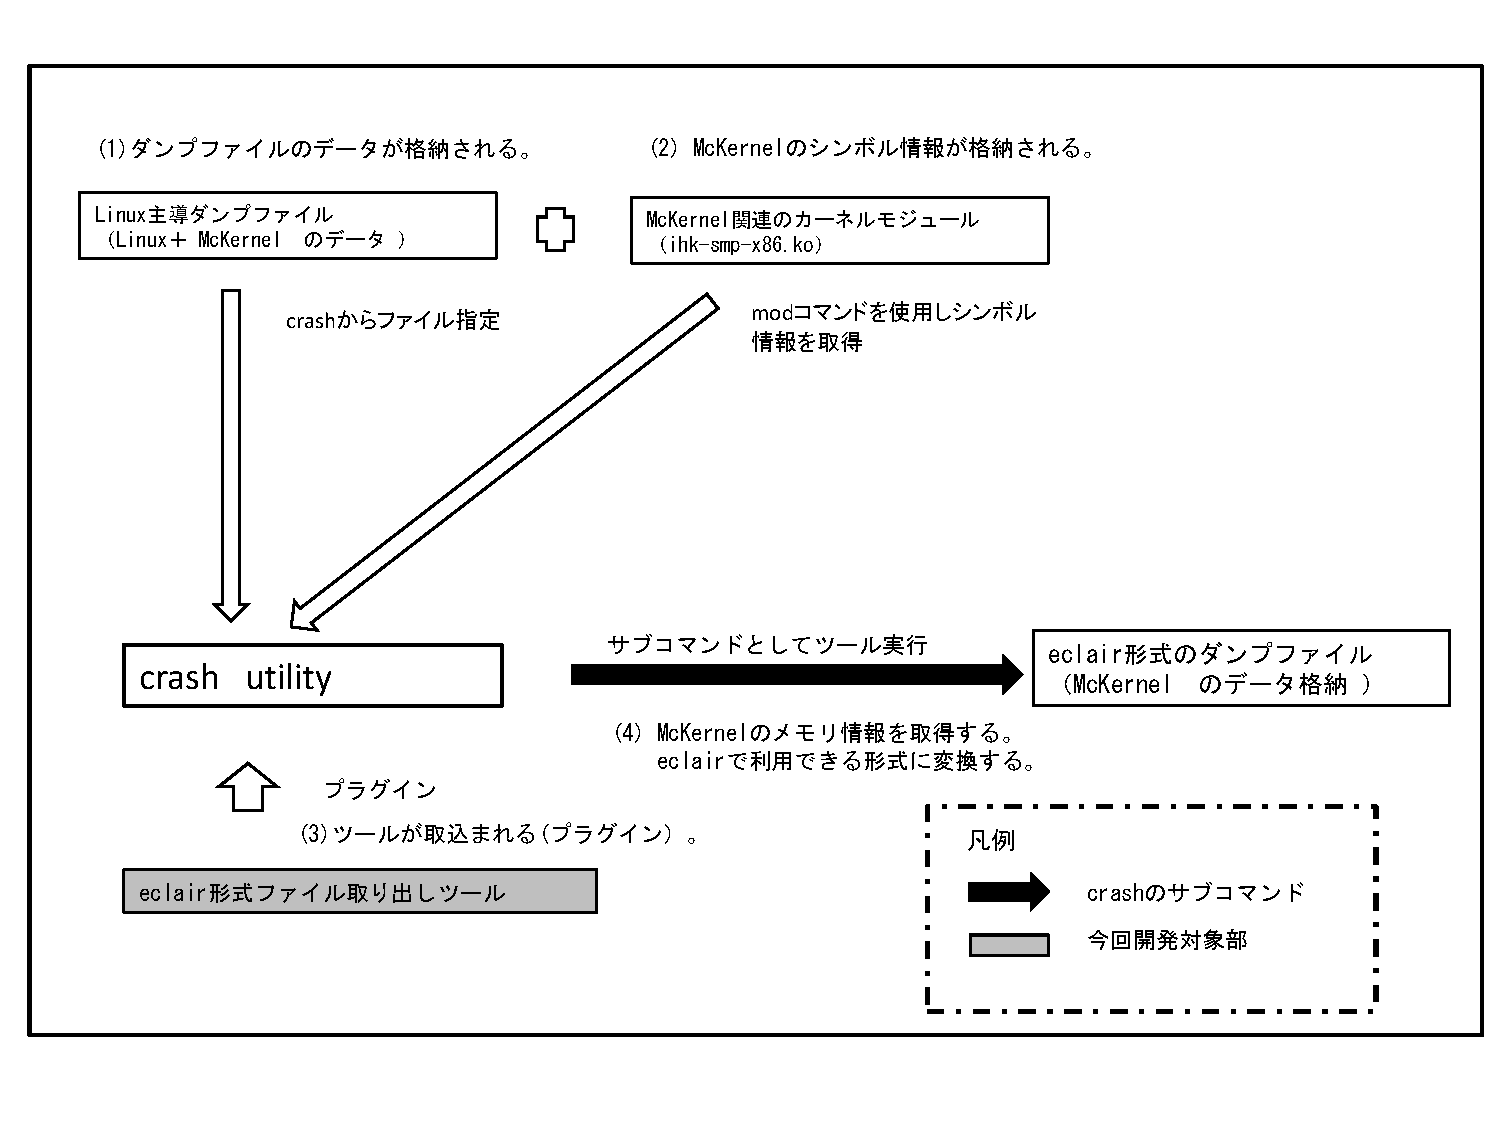
\includegraphics[scale=0.6]{figs/chap01_fig005.pdf}
  \caption{ダンプ形式変換処理の流れ}
  \label{figure:chap01_fig005}
\end{figure}
\FloatBarrier
%
ダンプ形式変換処理の流れを図\ref{figure:chap01_fig005}を用いて説明する。 
\begin{enumerate}
\renewcommand{\labelenumi}{(\arabic{enumi})}
\item crash内領域にダンプファイルのデータが格納される。\newline
コマンド:crash 〈vmlinuxのパス〉〈ダンプファイル(vmcore)のパス〉
\item crash内領域にIHKおよびMcKernelのカーネルモジュールのシンボル情報が格納される。\newline
コマンド:mod -s ihk-smp-x86 〈ihk-smp-x86.oのパス〉\newline
シンボル情報:dump\_page\_set\_addr(ダンプ対象ページリストのアドレス情報)
\item crash内にプラグインが取込まれる。\newline
コマンド:extend 〈crash utility extensionのパス (例:dump2mcdump.so)〉
\item ダンプ形式変換ツール(ldump2mcdump)を実行し、(2)のシンボル情報を用いて、McKernelに割り当てられた物理アドレス領域の情報を取得する。\newline
取得した情報を用いて、(1)からMcKernel関連情報を取り出し、eclair形式に整形して出力する。
\end{enumerate}

\subsection{\ADDAUGS{利用時の留意事項}}
\ADDAUGS{Linux主導ダンプはRHEL-7.4以降のバージョンのLinuxカーネルでのみ動作する。
また、Linuxのブートパラメタに\texttt{crash\_kexec\_post\_notifiers}を指定して、Linuxに、ファイルを生成する前に\texttt{panic\_notifier}に登録された関数を呼ばせる必要がある。}

\comment{
%==============================================================================
\subsection{\MODAUGS{Kernel Messages}}
%==============================================================================
McKernelのカーネルメッセージをMcKernel外部に出力する機能についてはバージョン1.1で詳細を検討するが、方針を説明する。

Linux上で動作するプロセス(\MODAUG{\texttt{ihkmond}}と呼ぶ)がMcKernelのカーネルメッセージが保存されているメモリエリアよりメッセージを取得して、Linux上で動作する\texttt{syslogd}にRFC 5424で規定されたフォーマットの構造体を作成して送信する。
\texttt{syslogd}側でメッセージをMcKernelが動作するノードで区別して分類したり、
複数McKernelインスタンスが1つのノードで動作している場合はインスタンスの番号で区別して分類したりできるようにする必要があるため、
\MODAUG{\texttt{ihkmond}}はこれらの情報を上記構造体の\texttt{HOSTNAME}フィールド、\texttt{PRI}フィールド、\texttt{STRUCTURED-DATA}フィールドに設定する。
具体的には、ホスト名が\texttt{host\_name}であるノードで動作するMcKernelの第$i$のインスタンスからのseverityが$s$であるカーネルメッセージに対しては、
\texttt{HOSTNAME}フィールドを\texttt{host\_name}に設定し、
McKernelを表すfacilityの番号を$f$、$p = f \times 8 + s$として、
\texttt{PRI}フィールドを\texttt{<}$p$\texttt{>}に設定し
\texttt{STRUCTURED-DATA}フィールドに\texttt{[mckernel instanceid=}\texttt{\char`\"}$i$\texttt{\char`\"}\texttt{]}を挿入し、
メッセージを格納するフィールドにMcKernelのカーネルメッセージを設定する。
なお、McKernelを表すfacilityの番号は\texttt{local0}から\texttt{local7}と呼ばれる16から23の整数のうちシステムで使われていないものを用いる。
% この値は他のメッセージとぶつからない値に決定する。
}

\comment{
\section{Support for Application Specific Kernels}
McKernel has been designed for the current HPC users with keeping
Linux API compatibility.  In other words, the selective kernel
services are supported by McKernel and the rest of services provided
by Linux are handled by Linux.
However, the selection of kernel serveices depends on users.
Thus, we assume that McKernel images are compiled for different specific
users, and the user may select one of the images for his/her purpose
at the job execution time.

The current McKernel is the following customizable features at the compile time.
\begin{enumerate}
\item CPU Scheduler
\item Eager/lazy phisical memory allocation
\end{enumerate}

In order to implement a new feature in McKernel for the future demands
that we have not known, we need some customizable feature for resource
managements such as process/thread and physical memory.
This feature is not yet designed in the specification version 1.2.
}

\comment{
% 例えば、
% 現在のIntel 64アーキテクチャ用McKernelのメモリ管理は、
% Linuxと同じcopy-on-writeや物理ページの動的な共有を実現するために、
% page構造体の大きな配列を持っており、
% 利用可能メモリの$\frac{1}{128}$のサイズを占めている。

そこで、特定のアプリケーションに合わせて、McKernelの機能を取り除いたり、
特定のアプリケーション向けの機能を追加したりすることを考えている。

このために、アプリケーションの性能に影響を与えることが予想される機能を
選び出し、それらのインターフェイスを定義し、それに従った実装をすること
で、異なる実装の開発や交換作業を容易にできるようにする。

この対象となる機能としては、プロセス空間管理、物理ページアロケータ、
threadのスケジューラなどが念頭にあるが、これに限らない。

機能の交換や追加は、ソースあるいはオブジェクトファイルの組み合わせを変
える、リコンパイルといった方法で行う。
}

\section{\MODAUG{プロセスダンプ}}
\MODAUG{McKernelではLinuxと同様の方法でプロセスのダンプファイルを生成できる。}
%プロセスは特定のシグナルを受け取ると、メモリ領域、レジスタなどのプロセス状態、\texttt{pid}などのプロセス情報を、\texttt{core}という名前のELF形式のファイルに出力する。

\comment{
プロセスがダンプを行うシグナルは以下の通り。
\begin{itemize}
\item SIGTRAP(\texttt{ptrace}システムコールによってトレースされていないない場合のみ)
\item SIGQUIT
\item SIGILL
\item SIGABRT
\item SIGFPE
\item SIGSEGV
\item SIGBUS
\item SIGSYS
\item SIGXCPU
\item SIGXFSZ
\end{itemize}
}

\subsection{\MODAUGS{実装の制限}}
出力される情報についての制限は以下の通り。
\begin{enumerate}
\item \MODAUG{複数スレッドが存在しても、親プロセスの情報しか出力しない。}
\item \texttt{NOTE}セグメントに格納されるプロセス状態(\texttt{struct elf\_prstatus64}型)のうち、以下のフィールドに対応する情報は格納しない。
\begin{verbatim}
    struct elf_siginfo pr_info;   /* シグナル情報 */
    short int pr_cursig;          /* 現在のシグナル */
    a8_uint64_t pr_sigpend;       /* ペンディングされているシグナル */
    a8_uint64_t pr_sighold;       /* holdされているシグナル */
    pid_t pr_pid;                 
    pid_t pr_ppid;                
    pid_t pr_pgrp;                
    pid_t pr_sid;                 
    struct prstatus64_timeval pr_utime;   /* ユーザ時間 */
    struct prstatus64_timeval pr_stime;   /* システム時間 */
    struct prstatus64_timeval pr_cutime;  /* 累積ユーザ時間 */
    struct prstatus64_timeval pr_cstime;  /* 累積システム時間 */
\end{verbatim}
なお、\texttt{struct elf\_siginfo}は以下のように定義される。
\begin{verbatim}
struct elf_siginfo {
    int si_signo; /* signal number */
    int si_code;  /* extra code */
    int si_errno; /* errno */
};
\end{verbatim}
\item \texttt{NOTE}セグメントに格納されるプロセス情報(\texttt{struct elf\_prpsinfo64}型)のうち、以下のフィールドに対応する情報は格納しない。
\begin{verbatim}
    char pr_sname;       /* プロセス状態(文字列)*/
    char pr_zomb;        /* Zombieか否か */
    char pr_nice;        /* Nice値 */
    a8_uint64_t pr_flag; /* フラグ */
    unsigned int pr_uid;
    unsigned int pr_gid;
    int pr_ppid, pr_pgrp, pr_sid;
    char pr_fname[16];           /* 実行可能ファイル名 */
    char pr_psargs[ELF_PRARGSZ]; /* 引数リスト先頭部分 */
\end{verbatim}
\end{enumerate}

\section{Utility Thread Offloading}\label{sec:uti}
McKernelは、スレッドをLinuxのCPUにマイグレートする機能を提供する。
この機能により、通信のプログレススレッドなどのヘルパースレッド(utility threadと呼ぶ)を、計算用CPU資源を利用することなく実行することができる。

\comment{
本機能はMPIライブラリなどミドルウェアに抽象化された機能を提供するライブラリ部と、実際の処理を行うカーネル部からなる。
ライブラリ部の処理ステップは以下の通り。
\begin{enumerate}
%\item ランタイムライブラリが、システムサービス用のCPUセットが環境変数\texttt{UTI\_CPU\_SET}に設定されていない場合は、Utility threadに使用するCPUセットを環境変数\texttt{UTI\_CPU\_SET}に設定する。設定されている場合は、必要に応じてその値を操作することでUtility threadに使用するCPUセットを設定する。
\item ランタイムライブラリが、\texttt{uti\_attr\_init()}でutility threadのCPUとNUMAノードの配置先(位置属性と呼ぶ)とスケジューラ観点での振る舞い(振る舞い属性と呼ぶ)を記述する属性オブジェクトを作成する。さらに、マクロを利用して位置属性と振る舞い属性を属性オブジェクトに書き込む。
\item ランタイムライブラリが、スレッド作成指示を\texttt{uti\_pthread\_create()}で出す。また、属性オブジェクトを引数としてOSに渡す。
\item McKernelが属性オブジェクトに従って適切なCPU、NUMAノード、スケジューリングポリシーを決定し、Linux CPUにスレッドを作成する
\item ランタイムライブラリが\texttt{uti\_attr\_destroy()}で属性オブジェクトを破壊する
\end{enumerate}
}

\comment{
処理ステップは以下の通り。
\begin{enumerate}
\item McKernelで実行中のユーザスレッドが、自スレッドをLinuxにマイグレートすることをシステムコールを用いて指示する。
\item McKernelは以下の処理を行う。
\begin{enumerate}
\item マイグレート対象のユーザスレッドのコンテキストを取得する。
\item McKernelからLinuxへのシステムコール委譲を用いて、mcexecに対して
スレッドのマイグレート指示を行う。このとき、取得したコンテキストを引き渡す。
\item システムコールの完了を待つ。\ADDAUG{なお、このシステムコールはLinuxへマイグレートされたスレッドが終了すると完了する。}
\item \MODAUG{\texttt{\_exit()}を用いて、前記システムコールの戻り値を自身のexit statusとしてMcKernelのスレッドを終了する。}
\end{enumerate}
\item mcexecはMcKernelからのスレッドマイグレート指示に対して以下の処理を行う。
\begin{enumerate}
\item システムコールワーカースレッドを新規に生成する。これは、自スレッドで
対応スレッドのコンテキストを処理するため、システムコールワーカースレッドが
不足するためである。生成したスレッドはシステムコール委譲待ちとなる。
\item 上記システムコールワーカースレッドがコンテキストをマイグレート対象スレッドの
コンテキストに切り替える。このとき、切り替え前のコンテキストを保存しておく。
切り替え前コンテキストを保存するのは、シグナル受信時やスレッド終了時に一時的
にmcexecのコンテキストに復帰する必要があるためである。
\item コンテキスト切り替え後、スレッドはマイグレート対象のスレッドとして、マイグレート指示のシステムコールからの戻りアドレスから処理を再開する。
\item マイグレート対象スレッドが発行するシステムコールのうち、McKernelへのオフロード(逆オフロードと呼ぶ)が必要なものを補足し、逆オフロード処理を行う。逆オフロードが必要なシステムコールは、\texttt{mmap, munmap, mprotect, brk, futex, gettid, exit, texit}である。処理は以下の通り。
\begin{enumerate}
  \item マイグレートしたスレッド(traceeと呼ぶ)をptraceシステムコールによりトレースするプロセス(tracerと呼ぶ)を生成する。
  \item tracerはtraceeにptraceで接続する。traceeはシステムコールを発行する度にtracerに報告するようになる。
  \item tracerは報告を受けた際、当該システムコールが逆オフロードが必要なものか否かを判断する。逆オフロードが必要である場合は対応する処理を行う。そして、traceeのレジスタを操作することでtraceeがシステムコールを呼び出さないようにしてからtraceeの実行を再開する。
\end{enumerate}
\end{enumerate}
\end{enumerate}
}

\comment{
\section{実装方針}
\subsection{実装の制約条件}
Linux CPUへのスレッド生成機能の実装は、以下の制約条件の下で行う。
\begin{itemize}
\item Linuxカーネル本体に対して改修を行わないこと
\item libcやlibpthreadなどのLinuxディストリビューションが提供するライブラリ
に対して改修を行わないこと
\end{itemize}

即ち、Linuxカーネルをはじめ、Linuxディストリビューションが提供する
パッケージ類を無改修の状態で、Linux CPUへのスレッド生成機能を利用可能とする
必要がある。

また、実装に際して、ユーザプログラムに対して以下の制約条件を課してよい。
\begin{itemize}
\item Linux CPUにマイグレートしたスレッドが発行可能なシステムコール
を制限する
\item Linux CPUにマイグレートしたスレッドを、再度McKernelに移動する
ことはできない
\end{itemize}
}

\comment{
\subsection{マイグレート指示処理}
McKernelで実行するユーザプログラムが、スレッドをLinuxにマイグレートすることを
指示する方法として、以下が考えられる。
\begin{enumerate}
\item CPUコアが不足した際に、スレッドの負荷状況などから自動的にLinux
にマイグレートするスレッドを選定する方法
\item システムコールによって、新たに生成する子スレッド、自スレッド、または、
他スレッドをLinuxにマイグレートすることを明示的に指示する方法
\end{enumerate}

本実装においては、Linuxにマイグレートしたスレッドに対して、システムコールの
利用制限が課せられるため、自動的にマイグレート対象スレッドを選定する方法は
採用できない(ユーザプログラムが正常に動作できなくなる可能性がある)。

このため、システムコールによって明示的にマイグレートするスレッドを指示する
方法を採用する。
但し、以下の理由により、マイグレート対象となるスレッドは、システムコールを
発行したスレッド、または、新たに生成する子スレッドのみを対象とする。
\begin{enumerate}
\item カーネルがスレッドを識別するにはスレッドIDが必要である
\item pthread\_create(3)によって生成したスレッドのスレッドIDを知るための
一般的な手段が存在しない(pthread\_t型からスレッドIDへの変換手段が無い)
\item pthreadライブラリを改修してスレッドID取得インタフェースを作成する
ことは、実装の制約条件に反するため実施しない
\item pthread\_create(3)以外の手段でスレッドを作成することは一般的では
ないため、スレッドIDによってマイグレート対象スレッドを指定する方法を
サポートしても利用される機会が著しく少なく、メリットが無いと考えられる
\end{enumerate}
}

\comment{
%--
新たに生成するスレッドをLinuxにマイグレートするには、
以下ように動作させれば良い。
\begin{enumerate}
\item スレッドをMcKernelコア上で実行を開始する。
\item Linux CPUへのマイグレートを指示する拡張システムコールを発行し、
カーネルモードにジャンプする。
\item Linuxへのシステムコール委譲を行い、制御をLinux CPUのmcexecに移動する。
\item mcexecにて、スレッドのエントリポイントにジャンプ。
\end{enumerate}
McKernel側でのカーネルモードへのジャンプは、
マイグレート指示の拡張システムコールで実現する。
制御のLinux CPUへの移動はMcKernelからLinuxへのシステムコール委譲を用いる。
エントリポイントへのジャンプは、マイグレート指示の拡張システムコールからの
戻りアドレスをエントリポイントに設定することで行う。
%--

%新たに生成するスレッドをLinuxにマイグレートするには、生成したスレッドに
%遷移する直前に、スレッド先頭アドレスからスレッドマイグレートのシステム
%コールが呼び出されたように動作すれば良い。具体的には、scheduleによって
%新しいスレッドのユーザ空間に処理が遷移する箇所で、システムコール戻り先
%をスレッド開始アドレスに指定してスレッドマイグレートのシステムコールを
%呼び出すことで実現できる。

新たなスレッドをpthread\_createなどのライブラリ呼び出し(ライブラリからclone(2)
が呼び出される)によって作成することを考慮し、clone(2)の動作を修飾する
システムコールを作成する。このシステムコールの指示によって、当該スレッドが
発行するclone(2)で 生成したスレッドの生成先をLinuxに切り替えることができる。
}

Linux CPUへのマイグレートは、以下の処理の組み合わせによって実現する。
\begin{enumerate}
%\item Mckernelで実行しているユーザプログラムにおいて、McKernelからLinuxにスレッドをマイグレートすることを指示する処理(マイグレート指示処理)
\item スレッドマイグレート処理\\McKernelで実行しているスレッドをLinux CPUにマイグレートする処理
\item システムコール処理\\Linuxにマイグレートしたスレッドの発行するシステムコールとMcKernelスレッドの発行するシステムコールとの一貫性を担保する処理
\item シグナル受信処理\\Linuxにマイグレートしたスレッドへシグナルを中継する処理
\item スレッド終了処理\\Linuxにマイグレートしたスレッドを正しく終了させる処理
\end{enumerate}

以下、それぞれの処理の概要を説明する。

\subsection{スレッドマイグレート処理}
スレッドマイグレートの処理のうち、McKernel側の処理は以下の通り。
\begin{enumerate}
\item McKernelで実行中のユーザスレッドが自スレッドをLinuxにマイグレートすることをシステムコールを用いて指示する。
\item McKernelはシステムコールを受けて以下の処理を行う。
\begin{enumerate}
\item マイグレート対象のユーザスレッドのコンテキストを取得する。
\item McKernelからLinuxへのシステムコール委譲を用いて、\texttt{mcexec}に対してスレッドのマイグレート指示を行う。このとき、取得したコンテキストを引き渡す。
\end{enumerate}
\item McKernelのスレッドはLinuxへマイグレートされたスレッドが終了するまでシステムコール完了を待ってスリープする。
\item McKernelはシステムコールが完了すると当該スレッドを起床する。
\item McKernelのスレッドはシステムコールの戻り値を引数として\texttt{\_exit}を呼び出し、スレッドを終了する。
\end{enumerate}

スレッドマイグレートの処理のうち、\texttt{mcexec}側の処理は以下の通り。
\begin{enumerate}
\item McKernelからスレッドマイグレート指示を受ける。
\item システムコールワーカースレッドを新規に生成する。これは、自スレッドで
マイグレートしたコンテキストを処理するため、システムコールワーカースレッドが
不足するためである。生成したスレッドはシステムコール委譲待ちとなる。なお、マイグレートは一回のみ可能であるため、システムコールワーカースレッドが必要以上に生成されることはない。
\item 当該スレッドの孫プロセスを生成する。当該孫プロセスは当該スレッドに\texttt{ptrace}システムコールを用いて接続し、当該スレッドが発行するシステムコールを捕捉する(次節で説明する)。
\item 自スレッドにおいて、コンテキストをマイグレート対象スレッドの
コンテキストに切り替える。このとき、切り替え前のコンテキストを保存しておく。
切り替え前コンテキストを保存するのは、シグナル受信時やスレッド終了時に一時的
にmcexecのコンテキストに復帰する必要があるためである。
\item コンテキスト切り替え後、スレッドはマイグレート対象のスレッドと
して、マイグレート指示のシステムコールからの戻りアドレスから処理を再開する。
\end{enumerate}

\comment{
コンテキストの詳細はアーキテクチャ依存である。
x86の場合、汎用レジスタ、スタックポインタ、インストラクションポインタ、
フラグレジスタ、TLSベース(MSR の FS\_BASE)を含む。
また、ページテーブルは mcexec のものを流用するため、コンテキストには含まない。

本実装においては、全ての汎用レジスタをコンテキストに含める。
x86の呼出規約により、
フラグレジスタや幾つかの汎用レジスタは、関数呼び出しやシステムコール呼び出しに
よって呼び出し前の値が保証されないことが規程されているため、
このようなレジスタはコンテキストに含めなくても良い(現在の実装では、
スレッドのマイグレートの契機はシステムコール呼び出しに限定されるため)。
しかし、将来他スレッドのマイグレートに対応する(マイグレート対象スレッドに割り込んで
マイグレート処理を開始する想定)ことに備えて、関数呼び出しで破壊されても良い
レジスタについてもコンテキストに含めておくことにした(このようなケースでは、
マイグレートの契機が関数呼び出しでは無いため、全ての汎用レジスタの値を保証する
必要がある)。

Linux側でのコンテキスト設定はmcexecから/dev/mcosへのioctl(2)発行の流れの中で
行うが、x86 Linuxのioctl(2)はユーザコンテキストを操作することができない。
正確には、x86 Linuxの場合、ユーザコンテキストを操作することができるのは、
ptrace(2)やrt\_sigreturn(2)などの一部のシステムコールに限られ、ioctl(2)は含まれ
ない。これは、x86 Linuxのシステムコール処理において、呼び出されたシステムコール
に従って退避するレジスタを変更しているためであり、ioctl(2)は一部の汎用レジスタ
しか退避されない(退避されないレジスタを使用する場合は、ioctlの処理内で適当な
スタック領域に退避される)。
このため、コンテキストの殆どについてはmcexecで設定を行い、MSRなどカーネルで設定
しなければならない部分のみ、別途システムコール(arch\_prctl(2))を発行して
設定する方式とする。
}

\subsection{システムコール処理}
Linuxにマイグレートしたスレッドが発行するシステムコールは捕捉し、必要に応じてMcKernelに処理を依頼する。
これは、システムコールの中には、\texttt{futex()}や\texttt{mmap()}など、McKernelの状態を操作するものがあるためである。

システムコールはptraceを用いて捕捉する。具体的には、マイグレート時にマイグレートしたスレッド(tracee)を監視するtracerプロセスをLinux上で生成し、traceeにシステムコールの発行を報告させる。また、tracerがtraceeのレジスタを操作することで必要に応じてLinux上でのシステムコール発行をスキップさせる。

システムコールごとの処理を\ref{tab:roffload}に示す。
\begin{table}[!h]
\footnotesize
\caption{マイグレートされたスレッドが発行するシステムコールの処理}\vspace{0.0em}
\label{tab:roffload}
\begin{tabular}{|p{0.40\linewidth}|p{0.55\linewidth}|} \hline
\multicolumn{1}{|c}{\textbf{システムコール}}&\multicolumn{1}{|c|}{\textbf{処理}}\\ \hline \hline
\textttw{mmap, mprotect, munmap, brk, futex}&IKCを用いてMcKernelに処理を依頼する \\ \hline
\texttt{getpid, gettid}&\texttt{mcexec}に記録しておいたidを返す\\ \hline
\texttt{open, read, write}などMcKernelからはシステムコール移譲を行うもの&Linux上でシステムコールを発行する\\ \hline
\texttt{exit\_group, \_exit}&\texttt{mcexec}で処理する\\ \hline
それ以外&エラー(ENOSYS)とする\\ \hline
\end{tabular}
\vspace{-0em}
\end{table}
\FloatBarrier

\subsection{シグナル受信処理}

\subsubsection{シグナル送信処理}

既存のMcKernelに、Linuxにシステムコールマイグレートしているプロセスに
対してMcKernelからシグナルを送信し、処理を中断する処理が存在する。
この処理を応用して、Linuxにマイグレートしたスレッドへのシグナル配送を実現する。

具体的には以下の処理を行う。
\begin{enumerate}
\item シグナル送信処理において、シグナル配送先スレッドがLinuxにマイグレート
されている場合、システムコールオフロード中スレッドへのシグナル送信と同様
にIKCを通じてmcexecにシグナル送信を依頼する。
\item mcexec はMcKernelのスレッドID(リモートスレッドID)から
Linux上のスレッドID(ローカルスレッドID)への変換を行い、
ローカルスレッドIDに対してシグナルを送信する。
\end{enumerate}

\comment{
mcexecの既存処理では、スレッドIDの対応をthread\_data配列を使って管理している。
Linuxへのスレッドマイグレートを実現するに当たり、mcexecのスレッド数は動的に変動
するため、thread\_dataを配列からリストに変更する。
}

\subsubsection{mcexecのシグナルハンドラ処理}

mcexecはLinuxからMcKernelのスレッドに送られたシグナルをMcKernelへ中継
するために、特別なシグナルハンドラを登録している。
このため、McKernelのスレッドからLinuxにマイグレートされたスレッドに送られる
シグナルに対応するシグナルハンドラの呼び出しは、直接行うことができず、
この特別なシグナルハンドラから行う必要がある。

mcexecのシグナルハンドラの入り口と出口では、TLSを切り替える必要がある。
TLSを切り替えない場合、Linuxにマイグレートされたスレッドの\texttt{errno}やその他のTLS領域
を破壊する可能性があるためである。
TLSの切り替えは、libc の arch\_prctlやsyscallを使用できない(これらは\texttt{errno}を更新
する)。TLSの切り替えはシステム依存の手段でシステムコールを呼び出す必要がある
(例えば、x86\_64ではsyscall命令の発行)。

TLSを切り替えるため、Linuxにマイグレートしているスレッドに対して
\texttt{mcctrl}においてmcexecのTLSとMcKernelスレッドのTLSを保持しておく。
TLS切り替え要求に対して通常のmcexecのスレッドは何もしないが、Linuxに
マイグレートされたスレッドでは、シグナルハンドラの入り口ではmcexecのTLSに
切り替え、出口ではMcKernelスレッドのTLSに切り替える。

\subsection{スレッド終了処理}
マイグレートされたスレッドの終了処理のステップは以下の通り。
\begin{enumerate}
\item スレッド終了の捕捉\\
マイグレートしたスレッドが\texttt{\_exit()}を呼び出した場合はtracerがptraceで補足し、シグナルによってスレッドが終了する場合は\texttt{mcctrl}がLinuxのスレッド終了フック(\texttt{trace\_sched\_process\_exit})を用いて捕捉する。
\item McKernel側でのスレッド終了\\
mcexecがIKCを用いてMcKernelにスレッドの終了ステータスを通知し、McKernel側のスレッドを終了させる。
\item Linux側でのスレッド終了\\
以下のステップでLinux側のスレッドを終了させる。
\begin{enumerate}
\item mcexecのスレッドのコンテキストを、マイグレートしたMcKernelスレッドのものから、\texttt{mcctrl}に記録しておいたマイグレート処理前のものへ切り替える。コンテキストの切り替えによって、\texttt{mcexec}の\texttt{ioctl()}の直後から実行が再開される。
\item tracerプロセスが終了する。
\item \texttt{mcexec}のスレッドが\texttt{\_exit()}を呼び出すことで終了する。
\end{enumerate}
\end{enumerate}

\subsection{実装詳細}
\subsubsection{Linux CPUへのスレッド生成の構成}

Linux CPUへのスレッド生成の構成を図\ref{figure:chap01_fig1}に示す。

\begin{figure}[!bh]
\begin{center}
\setlength{\unitlength}{3mm}
\begin{picture}(45, 30)(0, 0)

\put( 0,  0){\framebox(20, 30)[tl]{\small Linuxユーザ空間}}
\put( 0, 10){\line(20,  0){20}}
\put( 0,  0){\makebox(20, 10)[tl]{\small Linuxカーネル空間}}

\put( 1, 11){\framebox( 5,  17){}}
\put( 6, 11){\line(1, 0){4}}
\put(10, 11){\line(0, 1){6}}
\put( 6, 17){\line(1, 0){4}}
\put( 1, 11){\makebox( 5, 6){\small mcexec}}
\put( 6, 11){\makebox( 4, 6){\small libc}}
\put(1.5, 18){\framebox( 4, 9){\footnotesize\shortstack{tracer\\プロセス}}}
\put(5.5, 22.5){\vector(1, 0){2.5}}
\put( 7, 22.5){\makebox(0, 0)[b]{\tiny 制御}}

\put( 8, 18){\dashline[50]{0.3}(0, 0)(11, 0)(11, 10)(0, 10)(0, 0)}
\put( 8, 18){\makebox(11, 4){\small libc}}
%\put( 8, 22){\dashbox{0.4}(11, 0){}}
%\put(11, 25){\dashbox{0.4}( 8, 0){}}
%\put(11, 22){\dashbox{0.4}( 0, 3){}}
\put( 8, 22){\dashline[50]{0.3}(0, 0)(11, 0)}
\put(11, 25){\dashline[50]{0.3}(0, 0)(8, 0)}
\put(11, 22){\dashline[50]{0.3}(0, 0)(0, 3)}
\put(11, 22){\makebox( 5, 3){\small\shortstack{pthread\\など}}}
\put( 8, 25){\makebox(11, 3){\small ユーザプログラム}}

\put(25,  0){\framebox(20, 30)[tl]{\small McKernelユーザ空間}}
\put(25, 10){\line(20,  0){20}}
\put(25,  0){\makebox(20, 10)[tl]{\small McKernelカーネル空間}}

\put(33, 18){\framebox(11, 10){}}
\put(33, 18){\makebox(11, 4){\small libc}}
\put(33, 22){\line(1, 0){11}}
\put(36, 25){\line( 1, 0){8}}
\put(36, 22){\line( 0, 1){3}}
\put(36, 22){\makebox( 5, 3){\small\shortstack{pthread\\など}}}
\put(33, 25){\makebox(11, 3){\small ユーザプログラム}}

\put(19, 18){\vector(-1, 0){0}\dashline{0.2}(0, 0)(14, 0)}
\put(19, 28){\vector(-1, 0){0}\dashline{0.2}(0, 0)(14, 0)}
\put(20, 18){\makebox(5, 0)[b]{\small マップ}}
\put(20, 28){\makebox(5, 0)[b]{\small マップ}}

\put(1, 1){\framebox(9, 7){\small\shortstack{Linux\\カーネル}}}

\put(11, 1){\framebox(8, 7){}}
\put(11, 4){\line(1, 0){8}}
\put(11, 5){\makebox(8, 3){\small mcctrl}}
\put(11, 1){\makebox(8, 3){\small IHK}}

\put(26, 1){\framebox(18, 7){McKernel}}

\put(18, 26){\dottedline{0.1}(0, 0)(0, -24)(12, -24)}
\put(30,  2){\vector(1,  0){0}}
\put(20, 2){\makebox(5, 0)[b]{\small\shortstack{syscall\\呼び出し}}}

\put(18, 5){\dottedline{0.1}(0, 0)(-10, 0)}
\put(8,  5){\vector(-1,  0){0}}
\end{picture}

\caption{Linux CPUへのスレッド生成の構成}
\label{figure:chap01_fig1}
\end{center}

\end{figure}
\FloatBarrier

%\begin{itemize}
%\item \texttt{mcexec}はLinuxユーザ空間で動作する。
%\item Linuxカーネル、IHK、mcctrlはLinuxカーネル空間で動作する。
%\item ユーザプログラムは、libcやpthreadライブラリなど実行に必要なライブラリと共にMcKernelユーザ空間で動作する。
%\item McKernelはMcKernelユーザ空間で動作する。
ユーザプログラムのスレッドをLinux CPUに生成(実際はマイグレート)すると、ユーザプログラムが占めるメモリがLinuxユーザ空間にマップされ、Linuxユーザ空間の\texttt{mcexec}から参照可能となる。このとき、Linuxユーザ空間内には、\texttt{mcexec}のlibcとユーザプログラムのlibcが異なる実体として配置されている。

McKernelのスレッドをLinuxに生成するとき、\texttt{mcexec}の子プロセスとしてtracerプロセスを生成する。tracerプロセスはLinuxに生成したスレッドのシステムコールを監視し、Linux CPUのユーザプログラムが発行したシステムコールの一部(mmapなど)をmcctrl経由でMcKernel上で処理するように制御する。
%\end{itemize}


\subsubsection{\MODJULTWOS{\texttt{util\_indicate\_clone}システムコール}}
\texttt{util\_indicate\_clone}システムコールは自スレッドのthread構造体に\texttt{util\_indicate\_clone}システムコールの引数modとarg(カーネル空間にコピー済のarg)を設定する。
\comment{
\begin{enumerate}
\item 引数modがサポート外の値の場合、EINVALを返却。
\item \MODJULTWO{argが非NULLの場合、argの内容をユーザ空間からカーネル空間にコピーする。コピーに失敗した場合、EFAULTを返却する。}
\item  
\end{enumerate}
}

\texttt{thread}構造体の関連フィールドは以下のように定義される。
\small
\begin{verbatim}
struct thread {
    ... 略 ...
    int mod_clone;                // 生成対象OS
    void *mod_clone_arg;          // CPU位置の指示、スレッドの振る舞いの記述
};
\end{verbatim}
\normalsize

\subsubsection{\MODJULTWOS{\texttt{util\_migrate\_inter\_kernel}システムコール}}
util\_migrate\_inter\_kernelシステムコールは以下の処理を行う。
\begin{enumerate}
\item \MODJULTWO{argが非NULLの場合、argの内容をユーザ空間からカーネル空間にコピーする。コピーに失敗した場合、EFAULTを返却する。}
\item コンテキスト退避用ページを確保する。
\item コンテキスト退避用ページにユーザコンテキストを退避する。
\item コンテキスト退避用ページの物理アドレスを引数として、
sched\_setaffinityをオフロードする\footnote{他のシステムコール番号と被らない
ように、オフロード対象ではないsched\_setaffinityのシステムコール番号を
使用している。sched\_setaffinityをオフロードすると、
\texttt{mcexec}にてスレッドオフロード処理を行う}。
\item コンテキスト退避用ページを解放する。
\item sched\_setaffinityのオフロードの戻り値が正(成功)の場合、以下を行う。
\begin{enumerate}
\item 戻り値の0x100000000ビットが立っている場合、プロセスの終了を表すため、\texttt{terminate()}でプロセスを終了する。
\item それ以外の場合、\texttt{sched\_setaffinity()}の処理をもう一度McKernelに依頼することで、コンテキスト保存領域を\texttt{unmap}し、\texttt{do\_exit()}でスレッドを終了する。
\end{enumerate}
\item sched\_setaffinityのオフロードの戻り値が負(エラー)の場合、
戻り値を返却する。
\end{enumerate}

\subsubsection{\texttt{get\_system}システムコール}
\texttt{get\_system}システムコールはMcKernel上で実行すると0を返却する。
Linux上で実行すると、当該システムコールは存在しないため、\texttt{ENOSYS}でエラーリターンする。

\subsubsection{\texttt{clone}システムコール}
cloneシステムコールにて、子スレッドのthread構造体をrunqに接続する
(runq\_add\_thread呼び出し)前に以下の処理を行う。
\begin{enumerate}
\item 親スレッドのmod\_cloneに\texttt{SPAWN\_TO\_REMOTE}が設定されている場合、
子スレッドのthreadのmod\_cloneに\texttt{SPAWNING\_TO\_REMOTE}を設定する。
これにより、子スレッドをscheduleが処理するときにutil\_migrate\_inter\_kernelの処理が行われる。
\end{enumerate}

\subsubsection{\texttt{schedule}の処理}
scheduleに対して、以下の変更を行う。
\begin{enumerate}
\item nextを探す処理において、mod\_cloneに\texttt{SPAWNING\_TO\_REMOTE}が設定されている
スレッドがrunqに有る場合、そのスレッドを優先してnextに設定する。
\end{enumerate}

\subsubsection{\texttt{enter\_user\_mode}の処理}
enter\_user\_modeに対して、以下の変更を行う。
\begin{enumerate}
\item check\_signalを呼び出した後で、auto\_utilthr\_migrateを呼び出す。
この処理はcurrentスレッドに\texttt{SPAWNING\_TO\_REMOTE}が設定されている場合、
スレッドを開始する前にLinuxにマイグレートする。
\end{enumerate}

\subsubsection{\texttt{auto\_utilthr\_migrate}の処理}
auto\_utilthr\_migrateは以下の処理を行う。
\begin{enumerate}
\item currentスレッドのmod\_clone にSPAWINING\_TO\_REMOTEが設定されている場合、
mod\_cloneにSPAWN\_TO\_LOCALを設定し、
util\_migrate\_inter\_kernelを呼び出す。
これによって、新しいスレッドの開始前にutil\_migrate\_inter\_kernelシステム
コールの処理が実行される。
\end{enumerate}

\subsubsection{\texttt{do\_syscall}の処理}
do\_syscallに対して、以下の変更を行う。
\begin{enumerate}
\item オフロードしたシステムコールの状態が、STATUS\_SYSCALLの場合(Linuxから
McKernelへのシステムコール委譲)、以下の処理を行う。
\begin{enumerate}
\item システムコール番号がrt\_sigreturnの場合、シグナルハンドラの内容を
返却する。
\item システムコール番号がrt\_sigreturn以外の場合、以下を行う。
\begin{enumerate}
\item syscall\_tableを検索し、システムコール番号が登録されているか調べ、
登録されていない場合はENOSYSを返却する。
\item システムコールコンテキストを作成し、syscall\_tableに登録されている
システムコール処理を呼び出す。結果を返却する。
\end{enumerate}
\item システムコールの結果は、send\_syscall呼び出しによって、IKCを通じて
Linuxに通知する。この処理はremote page faultと同様である。
\end{enumerate}
\end{enumerate}

\subsubsection{\texttt{mcexec}の処理}
\texttt{mcexec}は以下の処理を行う。
\begin{enumerate}
%\item \texttt{thread\_data}を配列からリストに変更する。これに伴い、全スレッドをアクセスする処理をリストを辿るように変更する。
\item sched\_set\_affinity に対するオフロード処理として、以下を行う。
\begin{enumerate}
\item create\_worker\_createを呼び、新しいワーカースレッドを作成する。
このスレッドは、不足するシステムコールオフロードスレッドを補完するものである。
%
\comment{
mcexecのスレッドは\texttt{thread\_data\_s}構造体を用いて管理する。
\texttt{thread\_data\_s}構造体は以下のように定義される。
%従来のmcexecは、スレッド数固定のため、スレッドは\texttt{thread\_data\_s}構造体の配列として管理していたが、動的にマイグレートされたスレッドを追加する必要があるため、リストで管理するように変更する。
%\texttt{pthread\_join}を実施済みかどうかを保持するフラグを新設する。
\small
\begin{verbatim}
struct thread_data_s {
    struct thread_data_s *next;             // 次のスレッド
    ... 略 ...
    int joined;                             // join済み
} *thread_data;                             // リストの先頭
\end{verbatim}
\normalsize
}

\item \texttt{mcexec}スレッドとMcKernelスレッドのコンテキスト退避領域を作成する。
\item \texttt{mcctrl}にMcKernelスレッドのコンテキストをMcKernelスレッドのコンテキスト退避領域へコピーさせる(\texttt{MCEXEC\_UP\_UTIL\_THREAD1})。
\item tracerプロセスを生成する。tracerプロセスの詳細は4に示す。
\item \texttt{uti\_attr}が指定されている場合、\texttt{mcctrl}に\texttt{uti\_attr}処理を依頼する\\
(\textttw{MCEXEC\_UP\_UTI\_ATTR})。
\item 以下に示す\texttt{switch\_ctx}を行う。
%\texttt{switch\_ctx}は正常の場合、戻らない。
\begin{enumerate}
\item \texttt{mcexec}スレッドのコンテキスト退避領域に現在のコンテキストを退避する。
\item \texttt{mcctrl}にLinuxにマイグレートされたスレッドの情報を登録する\\(\texttt{MCEXEC\_UP\_UTIL\_THREAD2})。
\item コンテキストをマイグレートされたスレッドのコンテキストに切り替える。
%なお、\texttt{MCEXEC\_UP\_UTIL\_THREAD2}の帰り値は、0がローカルコンテキストへの切り替え完了を意味し、1がリモートコンテキストへの切り替え完了を意味する。
\end{enumerate}
\item マイグレートしたスレッドが完了した後に元のコンテキストに戻る。
\item \texttt{mcexec}スレッドのコンテキスト退避領域を解放する。
\item スレッドを終了する。
\end{enumerate}


\item シグナルを受信した際、シグナルハンドラにて以下の処理を行う。
\begin{enumerate}
\item \texttt{mcctrl}にMCEXEC\_UP\_SIG\_THREADを要求し、\texttt{mcexec}のTLSに切り替える。
\item \texttt{mcexec}のスレッドの場合、McKernelに受信したシグナルを通知する。
\item Linuxにマイグレートしたスレッドの場合は以下の処理を行う。
\begin{enumerate}
\item \texttt{mcctrl}にrt\_sigactionでMCEXEC\_UP\_SYSCALL\_THREAD要求を行い、
シグナルハンドラの設定を取得する。
\item シグナルハンドラがSIG\_IGNの場合、何もしない。
\item シグナルハンドラがSIG\_DFLの場合、シグナルがSIGCHLD、SIGURG、SIGCONT以外の
場合はシグナルハンドラを解除し、自プロセスにシグナルを送付する。これによって、
当該シグナルを受信して自プロセスが終了する。
\item シグナルハンドラがアドレスの場合、一時的にTLSを元に戻して
アドレスの関数(シグナルハンドラ)を呼び出す。
\end{enumerate}
\item \texttt{mcctrl}にMCEXEC\_UP\_SIG\_THREADを要求し、元のTLSに切り替える。
\end{enumerate}


\item tracerプロセスは以下の処理を行う。
\begin{enumerate}
\item traceeにて、tracerと待ち合わせに使用するパイプを作成する。
\item tracerプロセスをtraceeの孫プロセスとしてforkする。孫プロセスとするのはtraceeがtracerをwaitしないまま終了する場合に対応するためである。
\item traceeは以下の処理を行う。
\begin{enumerate}
\item tracerの予期せぬ終了を検知できるように、パイプの出力側を閉じる。
\item 子プロセスの終了を待つ。 子プロセスはすぐに終了する(孫プロセスがtracerになる)。
\item パイプの入力イベントの発生を(最大)1秒待つ(select)。
\item イベントが発生せずに1秒経過した場合、タイムアウトでエラーリターン。
\item selectがエラーの場合は、そのエラーコードでエラーリターン。
\item パイプから1バイト読み込み、パイプを閉じる。
\item パイプから1バイト読み込めなかった場合(EOF)、EAGAINでエラーリターン。
\item 正常にリターン。(以下、traceeスレッドはオフロード処理を継続する。)
\end{enumerate}
\item パイプの入力側を閉じる。
\item 子プロセスをforkし、親プロセスは終了(exit)する。子プロセスがtracerとなる。
\item /dev/mcos以外のファイルディスクリプタを全て閉じる。
\item 標準入出力を/dev/nullに割り当てる。
\item traceeスレッドにPTRACE\_ATTACHする。
\item traceeの停止を待つ(wait)。
\item PTRACE\_SYSCALL後の停止理由がシステムコールかシグナルかの区別を付ける
ために、PTRACE\_SETOPTIONSでPTRACE\_O\_TRACESYSGOODを指定する。
\item パイプに1バイト書き出し、パイプを閉じる。
\item 以下、無限ループ。
\begin{enumerate}
\item PTRACE\_SYSCALLによりtraceeを再開する。
\item traceeの停止を待つ(wait)。
\item traceeが終了した場合、終了コードをMcKernelに通知し、tracerを終了する。
\item 停止以外の場合、continue\footnote{停止以外の可能性としては、SIGCONTに
よる処理再開が考えられる。}。
\item システムコールで停止した場合、以下を行う。
\begin{enumerate}
\item PTRACE\_GETREGSを行い、traceeのレジスタを得る。
\item システムコール番号がioctlで引数にMCEXEC\_UP\_SYSCALL\_THREADが指定
されている場合、戻り値を逆オフロード結果に書き換える。
\item システムコール番号が逆オフロード対象で、
戻り値(x86の場合、rax)が--ENOSYSの場合(システムコール呼び出し時)、
システムコール番号をioctlに変更し、システムコール逆オフロードの引数を設定
する。
\item PTRACE\_SETREGSを行い、traceeのレジスタを更新する。
\end{enumerate}
\item システムコール以外(つまりシグナル)で停止した場合、次回PTRACE\_SYSCALL
に指定するシグナルとして、停止シグナルを設定する。
\end{enumerate}
\end{enumerate}

\end{enumerate}


\subsubsection{\MODJULTWOS{\texttt{mcctrl}の処理}}

\texttt{MCEXEC\_UP\_UTIL\_THREAD1}コマンドに対しては、McKernelから渡された物理アドレスで示されるMcKernelスレッドのコンテキストを、\texttt{mcexec}のコンテキスト退避領域にコピーする。

\texttt{MCEXEC\_UP\_UTIL\_THREAD2}コマンドに対しては、\texttt{host\_thread}構造体を作成する。
%fdに対応する\texttt{hanlderinfo}に接続する。

\comment{
\item システムコールアドレスの退避が行われていない場合、システムコールテーブル
からLinuxのシステムコールアドレスを退避する。
\item handlerinfoにhost\_thread構造体が未登録の場合、スレッド終了フックとして
process\_exit\_proberを登録する。
}
\comment{
\item システムコールテーブルにMcKernelのシステムコールアドレスを設定する。
}

\texttt{host\_thread}構造体はLinuxにマイグレートされたスレッドの情報を保持し、以下のように定義される。
\small
\begin{verbatim}
struct host_thread {
    struct host_thread *next;                // 同一PID内のリスト
    struct mcos_handler_info *handler;       // LWK情報へのハンドラ
    int pid;                                 // プロセスID
    int tid;                                 // スレッドID
    unsigned long usp;                       // mcexecコンテキストのSP
    unsigned long lfs;                       // mcexecのTLSベース
    unsigned long rfs;                       // ユーザプログラムのTLSベース
};
\end{verbatim}
\normalsize

\texttt{mcos\_handler\_info}はLWKの情報を保持し、以下のように定義される。
\small
\begin{verbatim}
strruct mcos_handler_info {
    int pid;
    int cpu;
    struct mcctrl_usrdata *ud;
    struct file *file;
};
\end{verbatim}
\normalsize

\comment{
\texttt{ihk\_file}構造体は\texttt{/dev/mcosX}に対するファイルディスクリプタインスタンスを管理する。
また、\texttt{mcos\_handler\_info}を\texttt{mcos\_data}に記録する。
\texttt{ihk\_file}構造体は以下のように定義される。
\begin{verbatim}
struct ihk_file {
    struct ihk_host_linux_os_data *osdata;    // OSインスタンス
    void (*release_handler)(ihk_os_t, void *);// リリースハンドラ
    void *param;                              // リリースハンドラの引数
    void *mcos_data;                          // LWK情報(追加)
};
\end{verbatim}
}

\subsubsubsection{\MODJULTWOS{MCEXEC\_UP\_UTI\_ATTRの処理}}
MCEXEC\_UP\_UTI\_ATTRの要求に対して、以下の処理を行う。
\begin{enumerate}
\item 初回の場合、以下を行う。
\begin{enumerate}
\item Linuxカーネル内のsched\_setaffinityとsched\_setscheduler\_nocheckの
アドレスを解決する。
\item ラウンドロビン管理用配列を確保し、0で初期化する。
\end{enumerate}
\item uti\_attrのフラグに、背反する組み合わせが指定されている場合、
エラーリターンする($-$ENOMEM)。
\item mcctrl\_usrdataのcpu\_topology\_listを辿って、McKernelにてcloneを発行した
スレッド(親スレッド)のMcKernelのCPU IDを持つCPUを検索する。
存在しない場合はエラーリターンする($-$EINVAL)。
\item 作業用のcpumaskを確保し、cpu\_active\_maskで初期化する。
確保できない場合、エラーリターンする($-$ENOMEM)。
\item 以下の処理によって、uti\_attrのフラグ指定に従い、割り当てるCPUの候補
を求め、作業用cpumaskに設定する。
\begin{enumerate}
\item フラグに\texttt{UTI\_FLAG\_NUMA\_SET}が設定されている場合、以下の処理を行う。
\begin{enumerate}
\item mcctrl\_usrdataのnode\_topology\_listを辿って、numa\_setに設定されている
NUMA IDと一致するNUMAノードを検索し、見付かったNUMAノードに属すCPUの和集合を
求める。
\item 作業用cpumaskとNUMAノードに属すCPU集合の積集合を求め、作業用cpumaskに
設定する。
\end{enumerate}
\item フラグに\texttt{UTI\_FLAG\_SAME\_NUMA\_DOMAIN}か\textttw{UTI\_FLAG\_DIFFERENT\_NUMA\_DOMAIN}
が設定されている場合、以下の処理を行う。
\begin{enumerate}
\item 全てのNUMAドメインについて、親スレッドが属しているかどうかを調べ、
\texttt{UTI\_FLAG\_SAME\_NUMA\_DOMAIN}が指定されている場合は当該ドメインに属すCPU集合の、
また、\texttt{UTI\_FLAG\_DIFFERENT\_NUMA\_DOMAIN}が指定されている場合には親スレッドが
属していないドメインのCPU集合の和集合を求める。
\item 作業用cpumaskとNUMAノードに属すCPU集合の積集合を求め、作業用cpumaskに
設定する。
\end{enumerate}
\item フラグに\texttt{UTI\_FLAG\_SAME\_L3}か\texttt{UTI\_FLAG\_DIFFERENT\_L3}が設定されており、
且つ、親スレッドのCPUがL3キャッシュと持つ場合、以下を行う。
\begin{enumerate}
\item \texttt{UTI\_FLAG\_SAME\_L3}が指定されている場合、キャッシュを共有するCPUの集合
を求める。
\item \texttt{UTI\_FLAG\_DIFFERENT\_L3}が指定されている場合、キャッシュを共有するCPUの
集合の補集合を求める。
\item 求めたCPU集合と作業用cpumaskの積集合を求め、作業用cpumaskに設定する。
\end{enumerate}
\item フラグに\texttt{UTI\_FLAG\_SAME\_L2}か\texttt{UTI\_FLAG\_DIFFERENT\_L2}が設定されており、
且つ、親スレッドのCPUがL2キャッシュと持つ場合、以下を行う。
\begin{enumerate}
\item \texttt{UTI\_FLAG\_SAME\_L2}が指定されている場合、キャッシュを共有するCPUの集合
を求める。
\item \texttt{UTI\_FLAG\_DIFFERENT\_L2}が指定されている場合、キャッシュを共有するCPUの
集合の補集合を求める。
\item 求めたCPU集合と作業用cpumaskの積集合を求め、作業用cpumaskに設定する。
\end{enumerate}
\item フラグに\texttt{UTI\_FLAG\_SAME\_L1}か\texttt{UTI\_FLAG\_DIFFERENT\_L1}が設定されており、
且つ、親スレッドのCPUがL1キャッシュと持つ場合、以下を行う。
\begin{enumerate}
\item \texttt{UTI\_FLAG\_SAME\_L1}が指定されている場合、キャッシュを共有するCPUの集合
を求める。
\item \texttt{UTI\_FLAG\_DIFFERENT\_L1}が指定されている場合、キャッシュを共有するCPUの
集合の補集合を求める。
\item 求めたCPU集合と作業用cpumaskの積集合を求め、作業用cpumaskに設定する。
\end{enumerate}
\end{enumerate}
\item 以下の処理によって、CPUアフィニティの設定、及び、スケジューラの設定を
行う。
\begin{enumerate}
\item 作業用cpumaskが空集合の場合は何もしない。
\item フラグに\texttt{UTI\_FLAG\_EXCLUSIVE\_CPU}が設定されている場合、以下の処理を
行う。
\begin{enumerate}
\item 作業用cpumaskからCPUを1つ選んでCPUアフィニティに設定する。
(CPUの選択方法は後述)
\item スケジューラにSCHED\_FIFOを設定する。
\end{enumerate}
\item フラグに\texttt{UTI\_FLAG\_CPU\_INTENSIVE}が設定されている場合、以下の処理を
行う。
\begin{enumerate}
\item 作業用cpumaskからCPUを1つ選んでCPUアフィニティに設定する。
(CPUの選択方法は後述)
\end{enumerate}
\item フラグに\texttt{UTI\_FLAG\_HIGH\_PRIORITY}が設定されている場合、以下の処理を
行う。
\begin{enumerate}
\item 作業用cpumaskからCPUを1つ選んでCPUアフィニティに設定する。
(CPUの選択方法は後述)
\item スケジューラにSCHED\_FIFOを設定する。
\end{enumerate}
\item フラグに\texttt{UTI\_FLAG\_NON\_COOPERATIVE}が設定されている場合、以下の処理を
行う。
\begin{enumerate}
\item 作業用cpumaskからCPUを1つ選んでCPUアフィニティに設定する。
(CPUの選択方法は後述)
\end{enumerate}
\item 以上に該当しない場合、作業用cpumaskの内容をCPUアフィニティに設定する。
\end{enumerate}
\item 作業用cpumaskを開放する。
\end{enumerate}


作業用cpumaskからCPUを1つ選択する手順を以下に示す。
\begin{enumerate}
\item ラウンドロビン管理用配列はCPU IDごとのマイグレートスレッド数を記録している。
この配列を用いて、作業用cpumaskに含まれかつマイグレートスレッド数が最小となるCPU IDを求める。
\item compare and swapによってラウンドロビン管理用配列を更新(1加算)する。
失敗した場合は、1から再度行う。
\item 更新したCPU ID以外の作業用cpumaskのビットをクリアする。
\end{enumerate}


\comment{
\subsubsubsection{MCEXEC\_UP\_SWITCH\_THREADの処理}
MCEXEC\_UP\_SWITCH\_THREADの要求に対して、以下の処理を行う。
\begin{enumerate}
\item 要求元スレッドがLinuxにマイグレートされたスレッドでない場合、
リターンする。
\item \_\_return\_syscallを呼び出して
util\_migrate\_inter\_kernelシステムコールの
戻り値に終了コードを設定する(但し、util\_migrate\_inter\_kernelは
ユーザプログラムに戻らない。この終了コードはスレッドの終了コードとして
設定される)。
\item handlerinfoから終了する要求元スレッドのhost\_thread構造体を切り離し、
解放する。
\comment{
\item handlerinfoにhost\_thread構造体が登録されていない場合、
システムコールテーブルのシステムコールアドレスを退避して
おいたLinuxのものに戻し、スレッド終了フックを解除する。
}
\end{enumerate}

\subsubsubsection{スレッド終了フック(process\_exit\_prober)の処理}
スレッド終了フック(process\_exit\_prober)は以下の処理を行う。
\begin{enumerate}
\item 終了したスレッドのPIDが\texttt{mcexec}のものでなければリターンする。
\item 終了したスレッドがLinuxにマイグレートされたスレッドでなければ
リターンする。
\item 終了したスレッドのtask\_structから終了コードを取得し、
\_\_return\_syscallを呼び出してutil\_migrate\_inter\_kernelシステムコールの
戻り値に設定する(但し、util\_migrate\_inter\_kernelはユーザプログラムに
戻らない。この終了コードはスレッドの終了コードとして設定される)。
\item handlerinfoから終了するスレッドのhost\_thread構造体を切り離し、
解放する。
\item handlerinfoにhost\_thread構造体が登録されていない場合、
システムコールテーブルのシステムコールアドレスを退避して
おいたLinuxのものに戻し、スレッド終了フックを解除する。
\end{enumerate}
}

\subsubsubsection{MCEXEC\_UP\_SIG\_THREADの処理}
MCEXEC\_UP\_SIG\_THREADの要求に対して、以下の処理を行う。
\begin{enumerate}
\item 要求元スレッドがLinuxにマイグレートされたスレッドでない場合、
EINVALでエラーリターンする。
\item 引数に従い、スレッドのFSベースアドレスを切り替える。
\end{enumerate}

\subsubsubsection{MCEXEC\_UP\_SYSCALL\_THREADの処理}
MCEXEC\_UP\_SYSCALL\_THREADの要求に対して、以下の処理を行う。
\begin{enumerate}
\comment{
\item システムコールがexitまたはexit\_groupの場合は、
MCEXEC\_UP\_SWITCH\_THREADの処理を呼び出してリターンする。
このとき、exit\_groupの場合は終了コードに0x100000000ビットを設定し、
プロセス終了を示す。
}
\item システムコール番号とシステムコール引数をsyscall\_request構造体に
設定する。
\item util\_migrate\_inter\_kernelの要求を検索する。存在しない場合は
ENOENTでエラーリターンする。
\item wait\_queue\_head\_list\_nodeを作成し、システムコールの結果待ちに
備える。
\item util\_migrate\_inter\_kernelのレスポンスにsyscall\_requestの物理アドレス
設定する。また、レスポンスの状態をシステムコール要求に設定する。
\item \_\_notify\_syscall\_requesterを呼び出して、McKernel側に
レスポンスの変更を通知する。
\item wait\_event\_interruptibleによって、システムコール完了を待つ。
\item 結果を返却する。
\end{enumerate}

\comment{
\subsubsection{システムコール処理}
システムコール処理は、Linuxのシステムコールテーブルを書き換える
ことによって呼び出される処理であり、mmap、munmap、mprotect、mremap、futex、
gettid、exit、exit\_group、fork、vfork、clone、execveが該当する。

システムコール処理は以下の処理を行う。
\begin{enumerate}
\item host\_threadに自スレッドが登録されているか調べる。
\item 自スレッドがhost\_threadに登録されていない場合、マイグレートされた
スレッドでは無いので、退避していたシステムコールアドレスに分岐する。
\item host\_threadに登録されている場合は、自スレッドがマイグレートされた
スレッドである。この場合、システムコールにより、以下を行う。
\begin{enumerate}
\item システムコールがfork、vfork、clone、execveの場合、マイグレートされた
スレッドでは利用できないので、ENOSYSでエラーリターンする。
\item システムコールがexit、exit\_groupの場合、スレッドまたはプロセスを
終了するため、MCEXEC\_UP\_SWITCH\_THREADの処理を呼び出す。
\item それ以外のシステムコールの場合は、McKernelにシステムコール委譲する。
\end{enumerate}
\end{enumerate}
}

\comment{
\subsubsection{IHKの処理}
IHKは以下の変更を行う。
\begin{enumerate}
\item ihk\_os\_set\_mcos\_private\_data関数の追加\\
指定されたfile構造体にLWK情報を登録する。
\item ihk\_os\_get\_mcos\_private\_data関数の追加\\
指定されたfile構造体に登録されているLWK情報を返却する。
\end{enumerate}
}

\subsection{実装の制限}
制限は以下の通り。
\begin{itemize}
\item Linux CPUにマイグレートしたスレッドに対してptraceシステムコールによるトレースは行えない。
\item Linux CPUにマイグレートしたスレッドが発行可能なシステムコールの種類は上記で説明したもののみである。
\item Linux CPUにマイグレートしたスレッドを、再度McKernelに移動することはできない。
\end{itemize}

\section{\MODMARS{高速プロセス起動}}
McKernelは、複数種のMPIプログラムを起動しさらにそれを繰り返すジョブにおいてMPIプログラム起動時間を短縮する機能を提供する。
\MODAUG{利用例としては、アンサンブルシミュレーションとデータ同化を繰り返す気象アプリケーションが挙げられる。}

起動時間の短縮は、それぞれのMPIプログラムを常駐させて、起動を停止状態からの復帰で置き換えることで実現する。
\ifx \HLDIFFAUG y
\RMAUG{また、停止時に物理メモリを後続MPIプログラムに明け渡す}\\\RMAUG{必要があるが、これはswapによって実現する。}
\fi
高速プロセス起動は以下の機能から構成される。
\begin{itemize}
\item \MODJULTWOS{プロセス実行停止および停止からの再開機能}\\
MPIプログラムが、本来プロセスとして終了するタイミングで終了せずに再開指示待ち状態で停止できるようにする。また、再開指示を受けて停止状態から復帰できるようにする。ライブラリ関数として実装する。
\ifx \HLDIFFAUG y
\item \RMAUG{Swap機能}\\
\RMAUG{停止前にメモリ内容をディスクに書き出す。システムコールとして実装する。}
\fi
\item \MODJULTWOS{MPIプログラムの繰り返し起動指示機能}\\
MPIプログラムの実行回数を把握し、初回は\texttt{mpiexec}を用いて起動し、2回目以降は停止しているプロセスを再開する。\texttt{ql\_mpiexec\_start}と呼ぶユーザコマンドとして実装する。
\item \MODJULTWOS{MPIプログラムの繰り返し起動からの終了指示機能}\\
再開指示待ち状態で停止しているMPIプロセスを終了させる。\texttt{ql\_mpiexec\_finalize}と呼ぶユーザコマンドとして実装する。
\end{itemize}

\comment{
\subsection{構成}
本機能に関係するコンポーネントとその動作概要を表\ref{tab:qlcomponent}に示す。
%
\begin{table}[!h]
\footnotesize
\caption{高速プロセス起動コンポーネント}\vspace{0.0em}
\label{tab:qlcomponent}
\begin{tabular}{|p{0.25\linewidth}|p{0.65\linewidth}|} \hline
\multicolumn{1}{|c}{\textbf{コンポーネント}}&\multicolumn{1}{|c|}{\textbf{説明}}\\ \hline \hline
\texttt{ql\_server}&\MODAUG{\texttt{ql\_mpiexec\_start}により起動される常駐プロセスで、\texttt{ql\_mpiexec\_\{start,finalize\}}からの指示を対象MPIプログラムに渡す。}\\ \hline
\ADDAUG{\texttt{ql\_talker}}&\ADDAUG{\texttt{ql\_mpiexec\_\{start,finalize\}}により\texttt{ql\_server}が動作するノードに起動されるプロセスで、\texttt{ql\_mpiexec\_\{start,finalize\}}と\texttt{ql\_server}との間のやり取りを仲介する。}\\ \hline
\texttt{ql\_mpiexec\_start}&\texttt{mpiexec}を置き換えるユーザ向けコマンドで、\texttt{ql\_server}と通信を行い、MPIプログラムが存在しない場合は起動し、存在している場合は停止状態から復帰させる。\\ \hline
\texttt{ql\_mpiexec\_finalize}&常駐しているMPIプログラムを終了させるユーザ向けコマンド。\\ \hline
\ADDAUG{\texttt{mpiexec監視プロセス}}&\ADDAUG{\texttt{ql\_mpiexec\_start}により起動される常駐プロセスで、\texttt{mpiexec}の標準入出力・エラー出力をリダイレクトするパイプを管理する。}\\ \hline
\texttt{ql\_client()}&\MODJULTWO{MPIプログラムが一回の計算が完了した時点で呼び出すライブラリ関数で、再開指示待ち、次回の計算のための引数および環境変数の設定を行う。}\\ \hline
\end{tabular}
\vspace{-0em}
\end{table}
\FloatBarrier

\comment{
\texttt{ql\_mpiexec\_start}の処理フローは以下の通り。
\begin{enumerate}
\item \MODJULTWO{ジョブスクリプトが\texttt{ql\_mpiexec\_start}でMPIプロセスに起動を指示する。\texttt{ql\_mpiexec\_start}は\texttt{mpiexec}を用いてMPIプロセスを起動する。}
\item 対象MPIプロセスが計算を行う。
\item 対象MPIプロセスが\RMAUG{swap-outを行ってから}再開指示待ち状態で停止する。
\item \MODJULTWO{ジョブスクリプトが\texttt{ql\_mpiexec\_start}でMPIプロセスに停止状態からの復帰を指示する。}
\item \MODJULTWO{対象MPIプロセスが停止状態から復帰し、swap-inを行う。}
\item \MODJULTWO{対象MPIプロセスがループ構造に従って、計算データ初期化処理直前のコード位置にジャンプする。}
\end{enumerate}

\texttt{ql\_mpiexec\_finalize}の実行処理フローは以下の通り。
\begin{enumerate}
\item \MODJULTWO{ジョブスクリプトが\texttt{ql\_mpiexec\_finalize}でMPIプロセスに実行の終了を指示する。}
\item 対象MPIプロセスが停止状態から復帰し、\texttt{MPI\_Finalize()}の処理および後続処理を行い、終了する。
\item 対象MPIプロセスの親である\texttt{mpiexec}が終了する。
\end{enumerate}
}

\subsection{全体フロー}
繰り返し実行と、繰り返しの終了とに分けて全体フローを説明する。

\begin{figure}[!t]
\centering
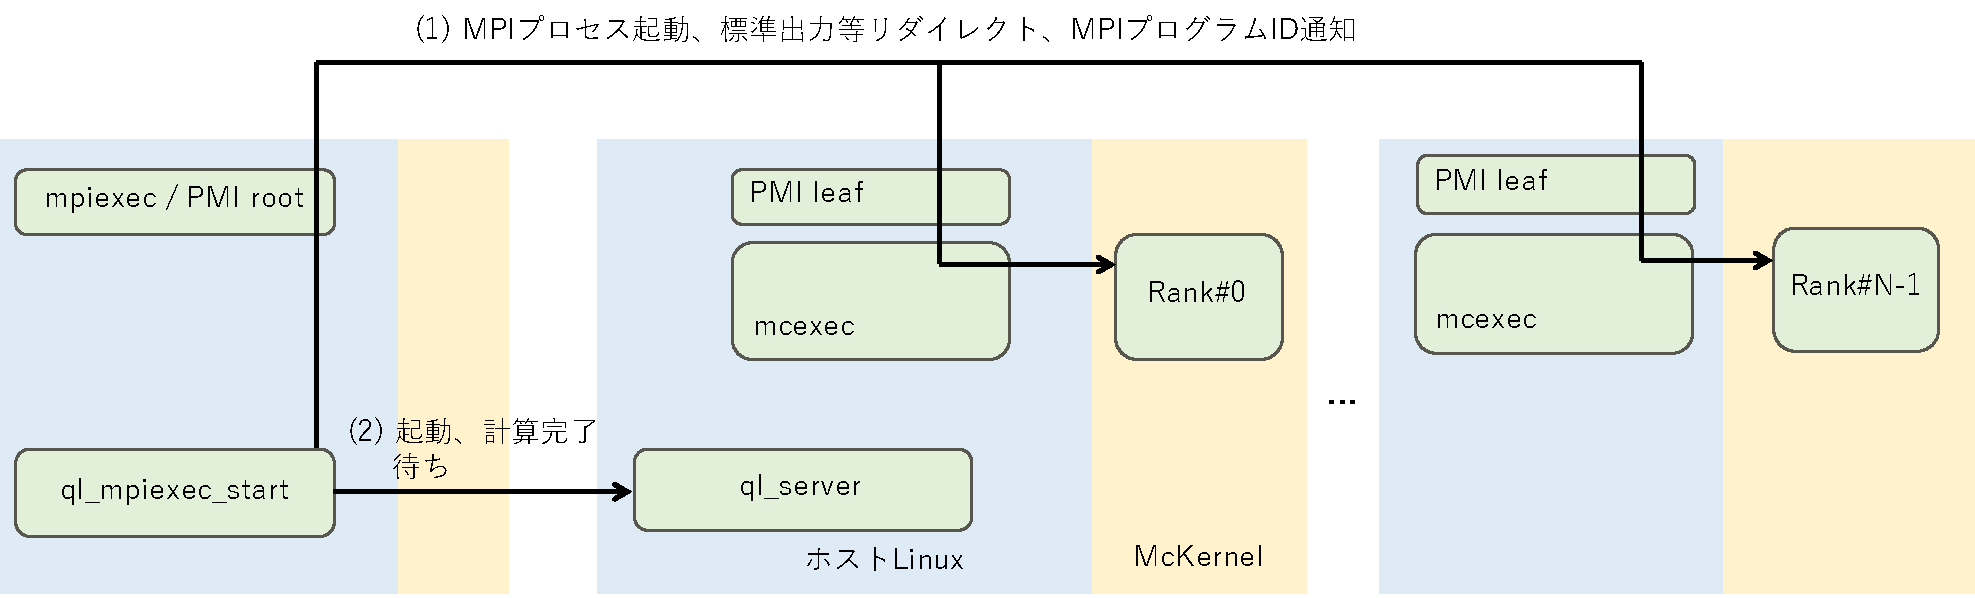
\includegraphics[width=0.95\linewidth]{figs/qlflowloop1.pdf}
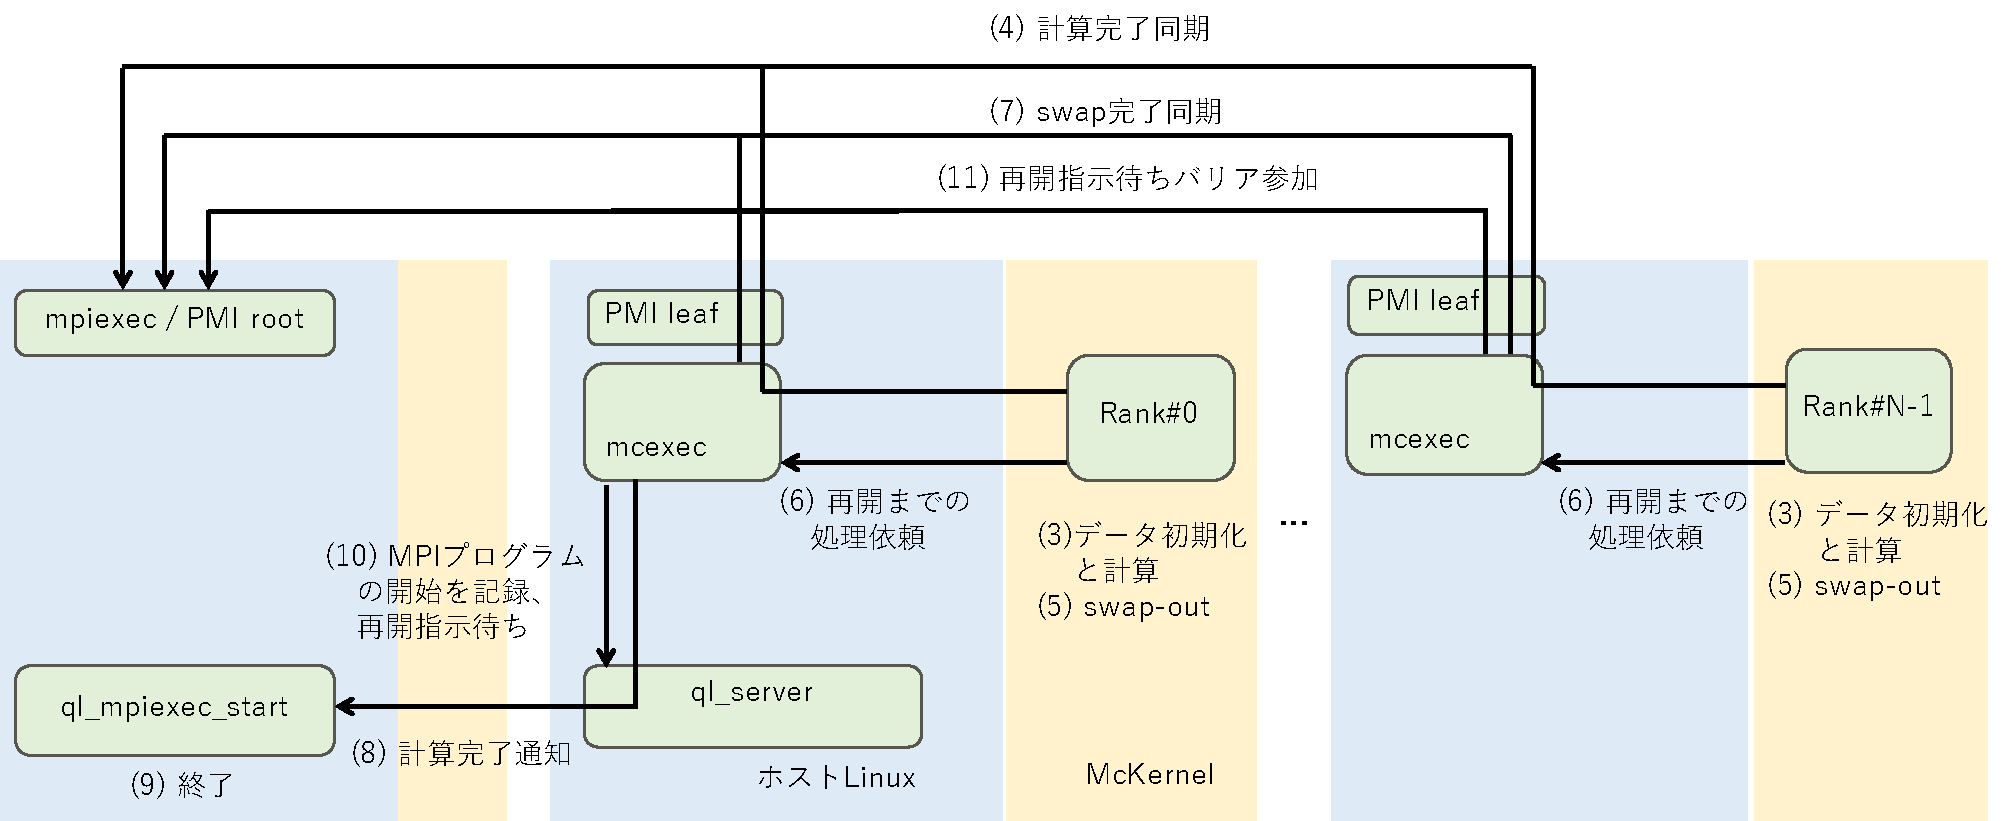
\includegraphics[width=0.95\linewidth]{figs/qlflowloop2.pdf}
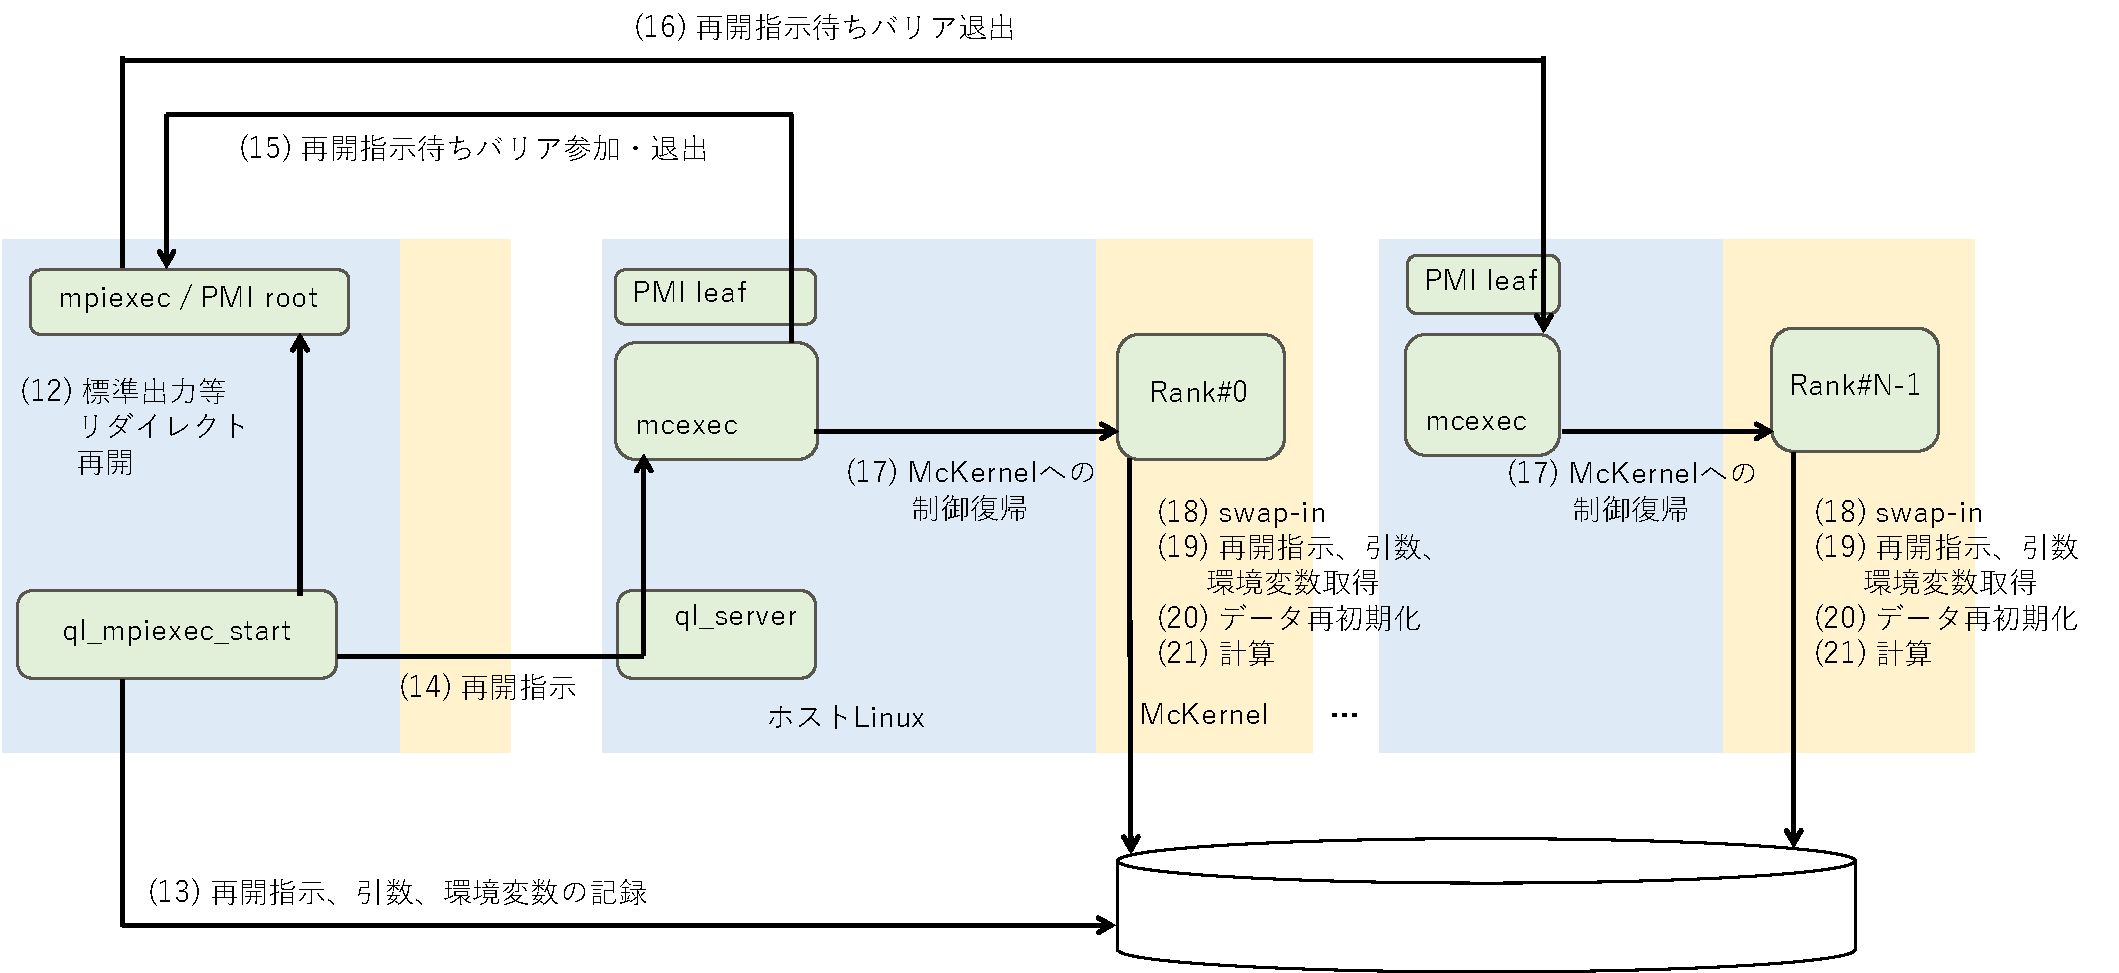
\includegraphics[width=0.95\linewidth]{figs/qlflowloop3.pdf}
\vspace{-0em}\caption{繰り返し実行のフロー}
\label{fig:qlflowloop}
\vspace{-0em}
\end{figure}
\FloatBarrier
%
繰り返し実行のフローを図\ref{fig:qlflowloop}を用いて説明する。
\begin{itemize}
\item[S01] ユーザが\texttt{ql\_mpiexec\_start}を実行し、MPIプログラムを起動する。\texttt{ql\_mpiexec\_start}は名前付きパイプを用いて\texttt{mpiexec}の標準入力、標準出力、標準エラーを自身のそれらとつなぐ。また、\texttt{ql\_server}で用いるMPIプログラムIDを実行可能ファイルとホストリストから生成し、環境変数でランク\texttt{\#0}に伝える。(図の(1))
\item[S02] \texttt{ql\_mpiexec\_start}が\texttt{ql\_server}の存在を確認し、存在しない場合は起動する。また、\texttt{ql\_server}に接続し、計算完了の通知を待つ。(図の(2))
\item[S03] 各ランクが引数と環境変数にもとづいてデータを初期化する。また、計算を行う。(図の(3))
\item[S04] 各ランクがPMIの機能を用いて計算完了の同期を行う。(図の(4))
\item[S05] 各ランクがカーネルモードに制御を移す。【未実装】また、swap-outを行う。(図の(5))
\item[S06] 各ランクのカーネルが\texttt{mcexec}に再開までの処理を依頼する。(図の(6))
\item[S07] 各ランクの\texttt{mcexec}がPMIの機能を用いて同期を行う。(図の(7))
\item[S08] ランク\texttt{\#0}の\texttt{mcexec}が計算完了を\texttt{ql\_server}経由で\texttt{ql\_mpiexec\_start}に通知する。(図の(8))
\item[S09] \texttt{ql\_mpiexec\_start}が終了する。(図の(9))
\item[S10] ランク\texttt{\#0}の\texttt{mcexec}がMPIプログラムの実行開始を\texttt{ql\_server}に記録し、また\texttt{ql\_server}からの再開指示待ち状態で停止する。MPIプログラムの実行開始を記録するのは、全MPIプログラムが終了した際に\texttt{ql\_server}を終了させるためである。(図の(10))
\item[S11] ランク\texttt{\#0}以外の全ランクの\texttt{mcexec}が再開指示待ちバリアに参加する。なお、ランク\texttt{\#0}の\texttt{mcexec}はこの時点で参加しないため、これらの\texttt{mexec}は停止する。(図の(11))
\item[S12] ユーザが\texttt{ql\_mpiexec\_start}を実行する。\texttt{ql\_mpiexec\_start}は\texttt{mpiexec}の名前付きパイプを用いた標準出力などのリダイレクトを再開する。(図の(12))
\item[S13] \texttt{ql\_mpiexec\_start}が再開指示、引数、環境変数をファイルに記録する。(図の(13))
\item[S14] \texttt{ql\_mpiexec\_start}が\texttt{ql\_server}経由でランク\texttt{\#0}の\texttt{mcexec}に再開を指示する。ランク\texttt{\#0}の\texttt{mcexec}は停止状態から復帰する。(図の(14))
\item[S15] ランク\texttt{\#0}の\texttt{mcexec}が再開指示待ちのバリアに参加する。またそのバリアから退出する。(図の(15))
\item[S16] \texttt{\#0}以外の全ランクの\texttt{mcexec}が停止状態から復帰し、再開指示待ちバリアから退出する。(図の(16))
\item[S17] 全ランクで\texttt{mcexec}からMcKernelのカーネルへ制御が戻る。(図の(17))
\item[S18] 【未実装】全ランクがswap-inを行う。また、カーネルからユーザプロセスに制御が戻る。(図の(18))
\item[S19] 全ランクがファイルを参照し再開指示を確認し、また新しい引数と環境変数を取得する。(図の(19))
\item[S20] 全ランクが新しい引数と環境変数にもとづいてデータを初期化する。(図の(20))
\item[S21] 全ランクが計算を行う。(図の(21))ステップS04に戻る。
\end{itemize}

\begin{figure}[!t]
\centering
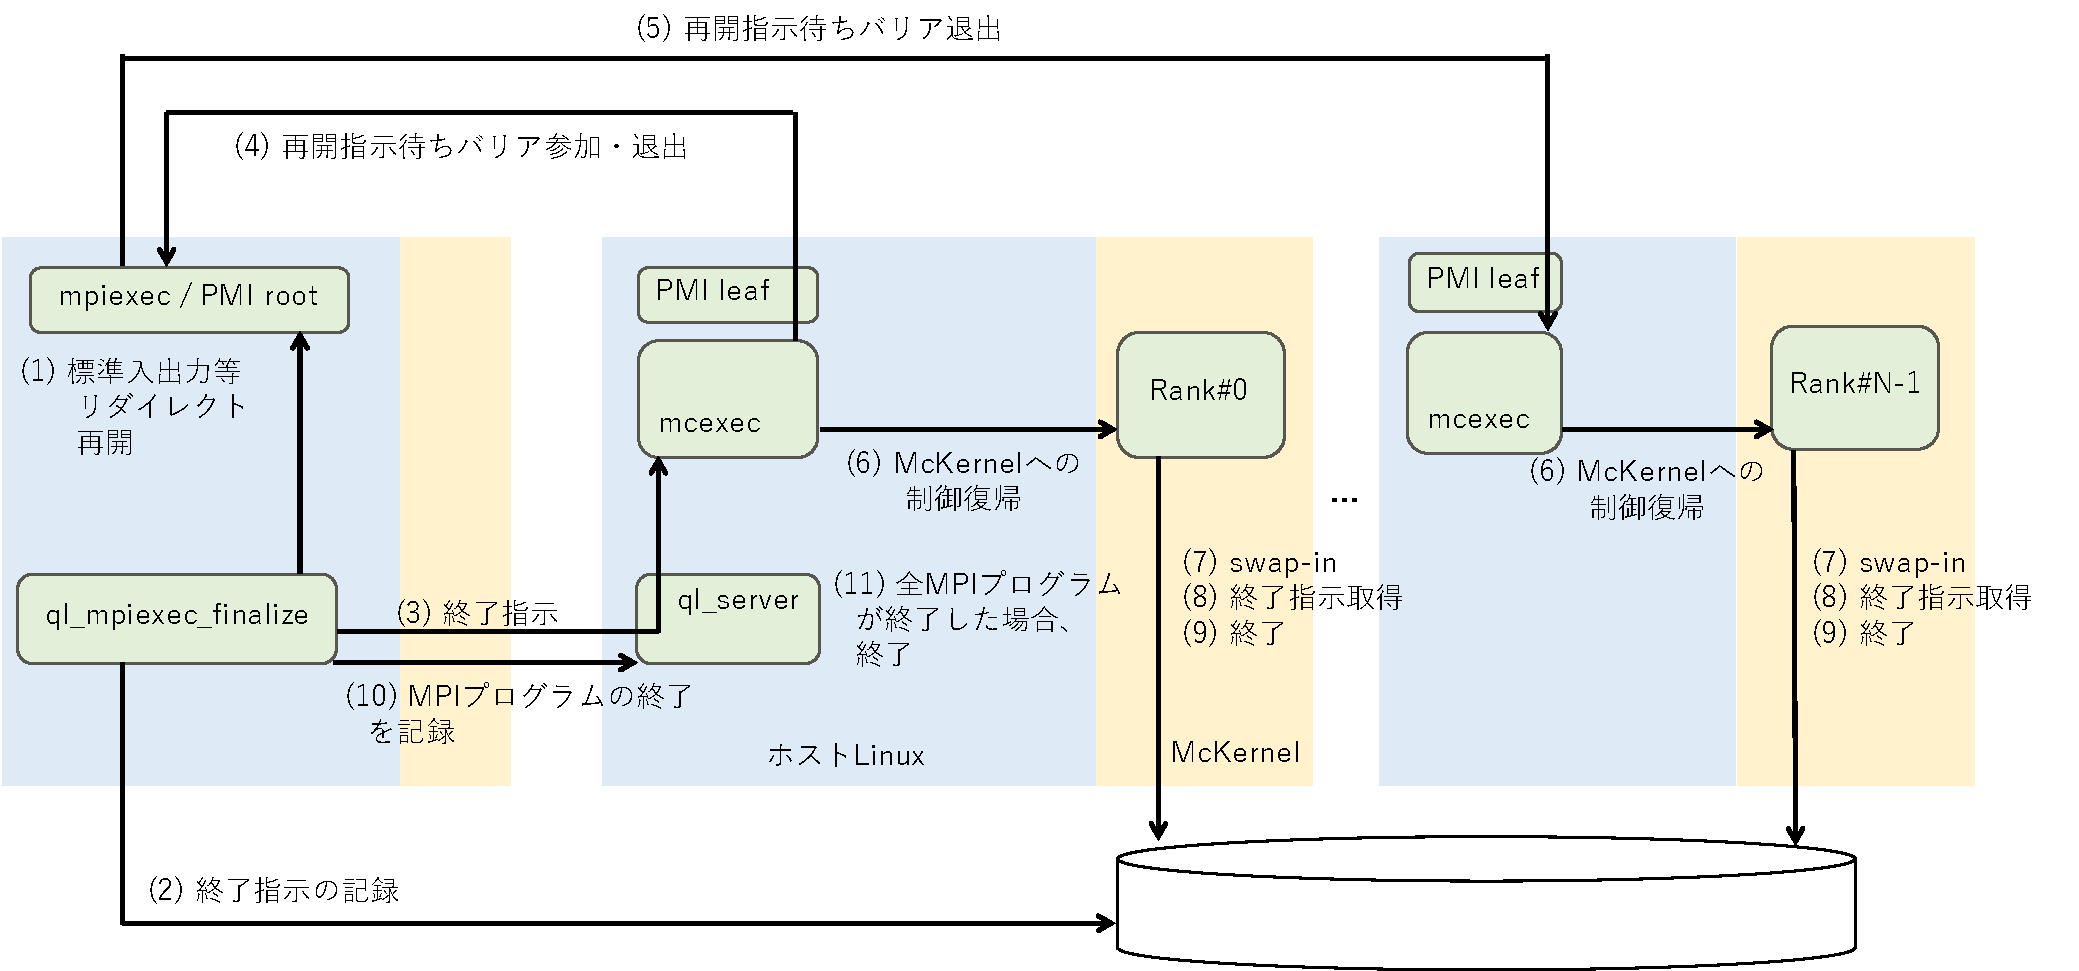
\includegraphics[width=0.95\linewidth]{figs/qlflowfin.pdf}
\vspace{-0em}\caption{繰り返し終了のフロー}
\label{fig:qlflowfin}
\vspace{-0em}
\end{figure}
\FloatBarrier
%
繰り返し終了のフローを図\ref{fig:qlflowfin}を用いて説明する。
\begin{itemize}
\item[S101] ユーザが\texttt{ql\_mpiexec\_finalize}を実行する。\texttt{ql\_mpiexec\_finalize}は\texttt{mpiexec}の名前付きパイプを用いた標準出力などのリダイレクトを再開する。(図の(1))
\item[S102] \texttt{ql\_mpiexec\_finalize}は終了指示をファイルに記録する。(図の(2))
\item[S103] \texttt{ql\_mpiexec\_finalize}が\texttt{ql\_server}経由でランク\texttt{\#0}の\texttt{mcexec}にMPIプログラムの終了を指示する。ランク\texttt{\#0}の\texttt{mcexec}は停止状態から復帰する。(図の(3))
\item[S104] ランク\texttt{\#0}の\texttt{mcexec}が再開指示待ちのバリアに参加する。また、バリアから退出する。(図の(4))
\item[S105] ランク\texttt{\#0}以外の全ランクの\texttt{mcexec}が停止状態から復帰し、再開指示待ちバリアから退出する。(図の(5))
\item[S106] 全ランクで\texttt{mcexec}からMcKernelのカーネルへ制御が戻る。(図の(6))
\item[S107] 【未実装】全ランクがswap-inを行う。また、カーネルからユーザプロセスに制御が戻る。(図の(7))
\item[S108] 全ランクがファイルを参照して終了指示を確認する。(図の(8))
\item[S109] 全ランクが終了する。(図の(9))
\item[S110] \texttt{ql\_mpiexec\_finalize}が全ランクの終了をwait()などで検知し、MPIプログラムの実行終了を\texttt{ql\_server}に記録する。(図の(10))
\item[S111] \texttt{ql\_server}は全MPIプログラムが終了していた場合、終了する。(図の(11))
\end{itemize}
\FloatBarrier
}

以下、これらの機能の詳細を説明する。

\subsection{\ADDAUGS{詳細}}
%高速プロセス起動は、MPIプログラムが各回の計算完了後に次回の計算開始の指示待ち状態に入るようにした上で、ジョブスクリプトから\texttt{ql\_mpiexec\_start}コマンドで計算開始を指示することで実現する。
%\texttt{ql\_mpiexec\_start}はMPIプログラムを管理するプロセス、\texttt{ql\_server}を起動し、\texttt{ql\_server}経由でMPIプロセスに指示を出す。

関連プロセスを表\ref{tab:qlprocess}示す。
\begin{table}[!ht]
\footnotesize
\caption{プロセス一覧}\vspace{0.0em}
\label{tab:qlprocess}
\begin{tabular}{|p{0.20\linewidth}|p{0.75\linewidth}|} \hline
\multicolumn{1}{|c|}{\textbf{プロセス}}&\multicolumn{1}{c|}{\textbf{説明}}\\ \hline 
 \hline
\texttt{ql\_mpiexec\_start}&ユーザがジョブスクリプトに記述して用いる、各回の計算開始を指示するコマンドである。指示は\texttt{ql\_talker}と\texttt{ql\_server}を経由してMPIプログラムに送られる。なお、一回の計算が完了すると、本コマンドは終了する。\\ \hline
\texttt{ql\_mpiexec\_finalize}&ユーザがジョブスクリプトに記述して用いる、MPIプログラムの実行終了を指示するコマンドである。指示は\texttt{ql\_talker}と\texttt{ql\_server}を経由してMPIプログラムに送られる。なお、MPIプログラムの終了と共に本コマンドは終了する。\\ \hline
\texttt{mpiexec}監視&\texttt{mpiexec}プロセスの起動、死活監視、標準入出力およびエラー出力のリダイレクトを行う。本プロセスは\texttt{ql\_mpiexec\_start}コマンドより起動され常駐する。また、\texttt{mpiexec}プロセス終了と共に終了する。\\ \hline
\texttt{mpiexec}&MPIプロセスを生成する。本プロセスは\texttt{mpiexec}監視プロセスの子プロセスとして起動される。すべてのランク終了と共に終了する。\\ \hline
\texttt{mcexec}&ホストLinux上でMcKernelのユーザプログラムプロセスを生成・管理する。\\ \hline
\texttt{ql\_server}&高速プロセス起動対象のMPIプログラムを記録し、\texttt{ql\_mpiexec\_\{start,finalize\}}コマンドの指示をMPIプロセスに送る。\texttt{ql\_server}は\texttt{ql\_mpiexec\_start}コマンドから\texttt{ssh}で起動され常駐する。また、高速プロセス起動対象のMPIプログラムが全て終了した時点で終了する。\\ \hline
\texttt{ql\_talker}&\texttt{ql\_mpiexec\_\{start,finalize\}}と\texttt{ql\_server}との間の通信を仲介する。\texttt{ql\_mpiexec\_\{start,finalize\}}コマンドから\texttt{ssh}で\texttt{ql\_server}が実行されている計算ノードに起動される。本プロセスは指示完了と共に終了する。\\ \hline
\end{tabular}
\vspace{-0em}
\end{table}
\FloatBarrier

プロセス構成を図\ref{fig:ProcessDiagram}に示す。
\begin{figure}[!ht]
\centering
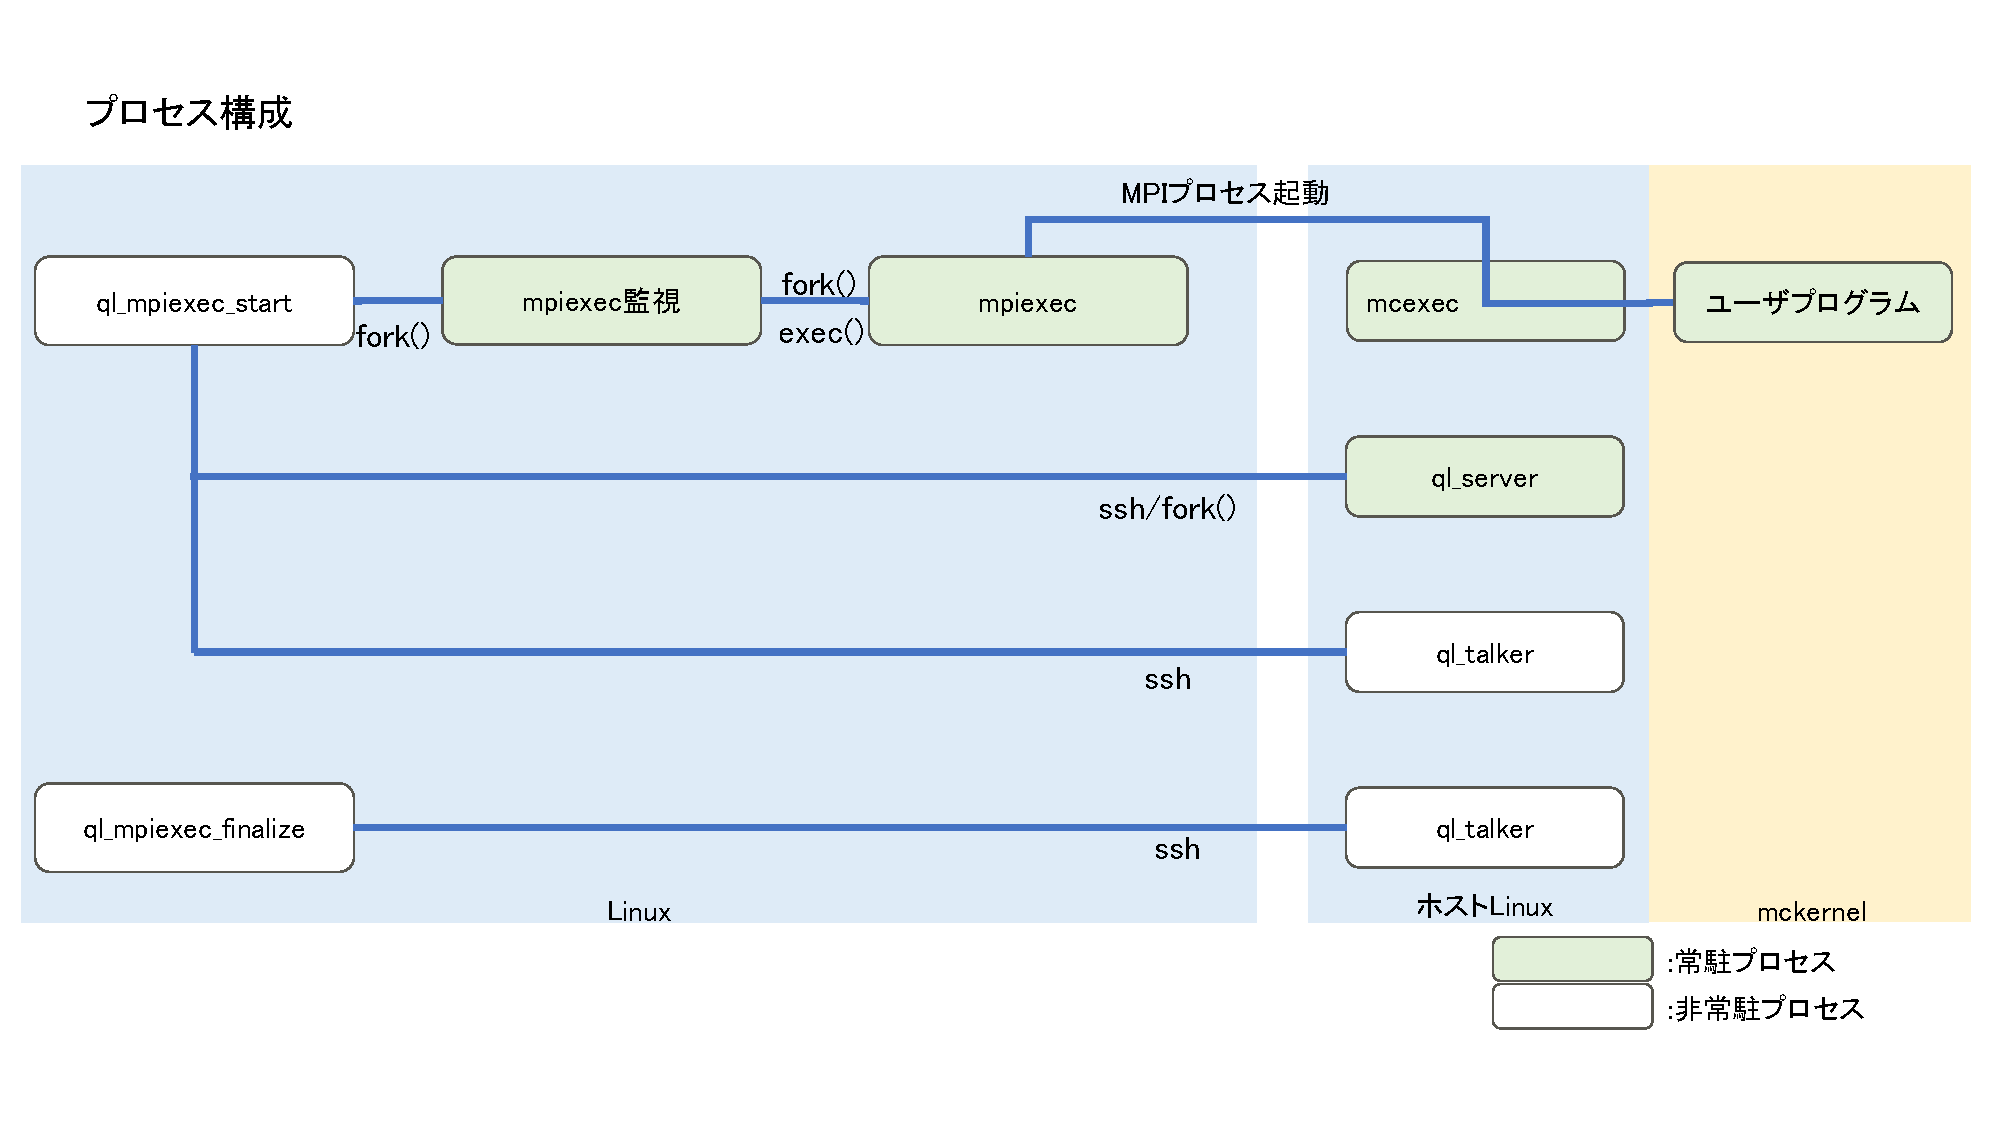
\includegraphics[width=0.95\linewidth]{figs/ProcessDiagram.pdf}
\vspace{-0em}\caption{プロセス構成}
\label{fig:ProcessDiagram}
\vspace{-0em}
\end{figure}
\FloatBarrier

プロセス間通信で用いるコマンドは以下の通り。
\begin{table}[!ht]
\footnotesize
\begin{tabular}{|p{0.10\linewidth}|p{0.15\linewidth}|p{0.70\linewidth}|} \hline
\multicolumn{1}{|c}{\textbf{コマンド}}&\multicolumn{1}{|c|}{\textbf{ マクロ}}&\multicolumn{1}{c|}{\textbf{説明}}\\ \hline 
 \hline
\texttt{Eコマンド}&\texttt{QL\_EXEC\_END}&\texttt{mcexec}が\texttt{ql\_server}経由で\texttt{ql\_mpiexec\_start}へ各回の計算完了を通知する際に用いる\\ \hline
\texttt{Fコマンド}&\texttt{QL\_RET\_FINAL}&\texttt{mpiexec監視}プロセスが\texttt{ql\_server}へMPIプログラムの終了を通知する際に用いる\\ \hline
\texttt{Rコマンド}&\texttt{QL\_RET\_RESUME}&\texttt{ql\_server}が\texttt{mcexec}へ待ち状態からの起床を指示する際に用いる\\ \hline
\texttt{Nコマンド}&\texttt{QL\_COM\_CONN}&\texttt{ql\_mpiexec\_start}が\texttt{ql\_server}にMPIプログラムの登録を依頼する際に用いる\\ \hline
\texttt{Aコマンド}&\texttt{QL\_AB\_END}&\texttt{ql\_server}が他プロセスからのコマンドを処理する際に、コマンド転送先プロセスを見つけられなかった場合に返答として用いる\\ \hline
\end{tabular}
\vspace{-0em}
\end{table}
\FloatBarrier

プロセス間通信の通信電文フォーマットは以下の通り。
\begin{verbatim}
<コマンド> <データサイズ> <データ>
\end{verbatim}

各フィールドのサイズ、意味は以下の通り。
\begin{table}[!ht]
\footnotesize
\begin{tabular}{|p{0.20\linewidth}|p{0.10\linewidth}|p{0.60\linewidth}|} \hline
\multicolumn{1}{|c}{\textbf{フィールド}}&\multicolumn{1}{|c|}{\textbf{サイズ}}&\multicolumn{1}{c|}{\textbf{説明}}\\ \hline 
 \hline
\texttt{<コマンド>}&1~byte&コマンド\\ \hline
\texttt{<データサイズ>}&4~byte&byte単位のデータサイズを表す16進数文字列\\ \hline
\texttt{<データ>}&可変&データを表す文字列\\ \hline
\end{tabular}
\vspace{-0em}
\end{table}
\FloatBarrier

関連コマンドと関連プロセスの動作フローを図\ref{fig:SequenceDiagram}を用いて説明する。
%
\begin{figure}[!t]
\centering
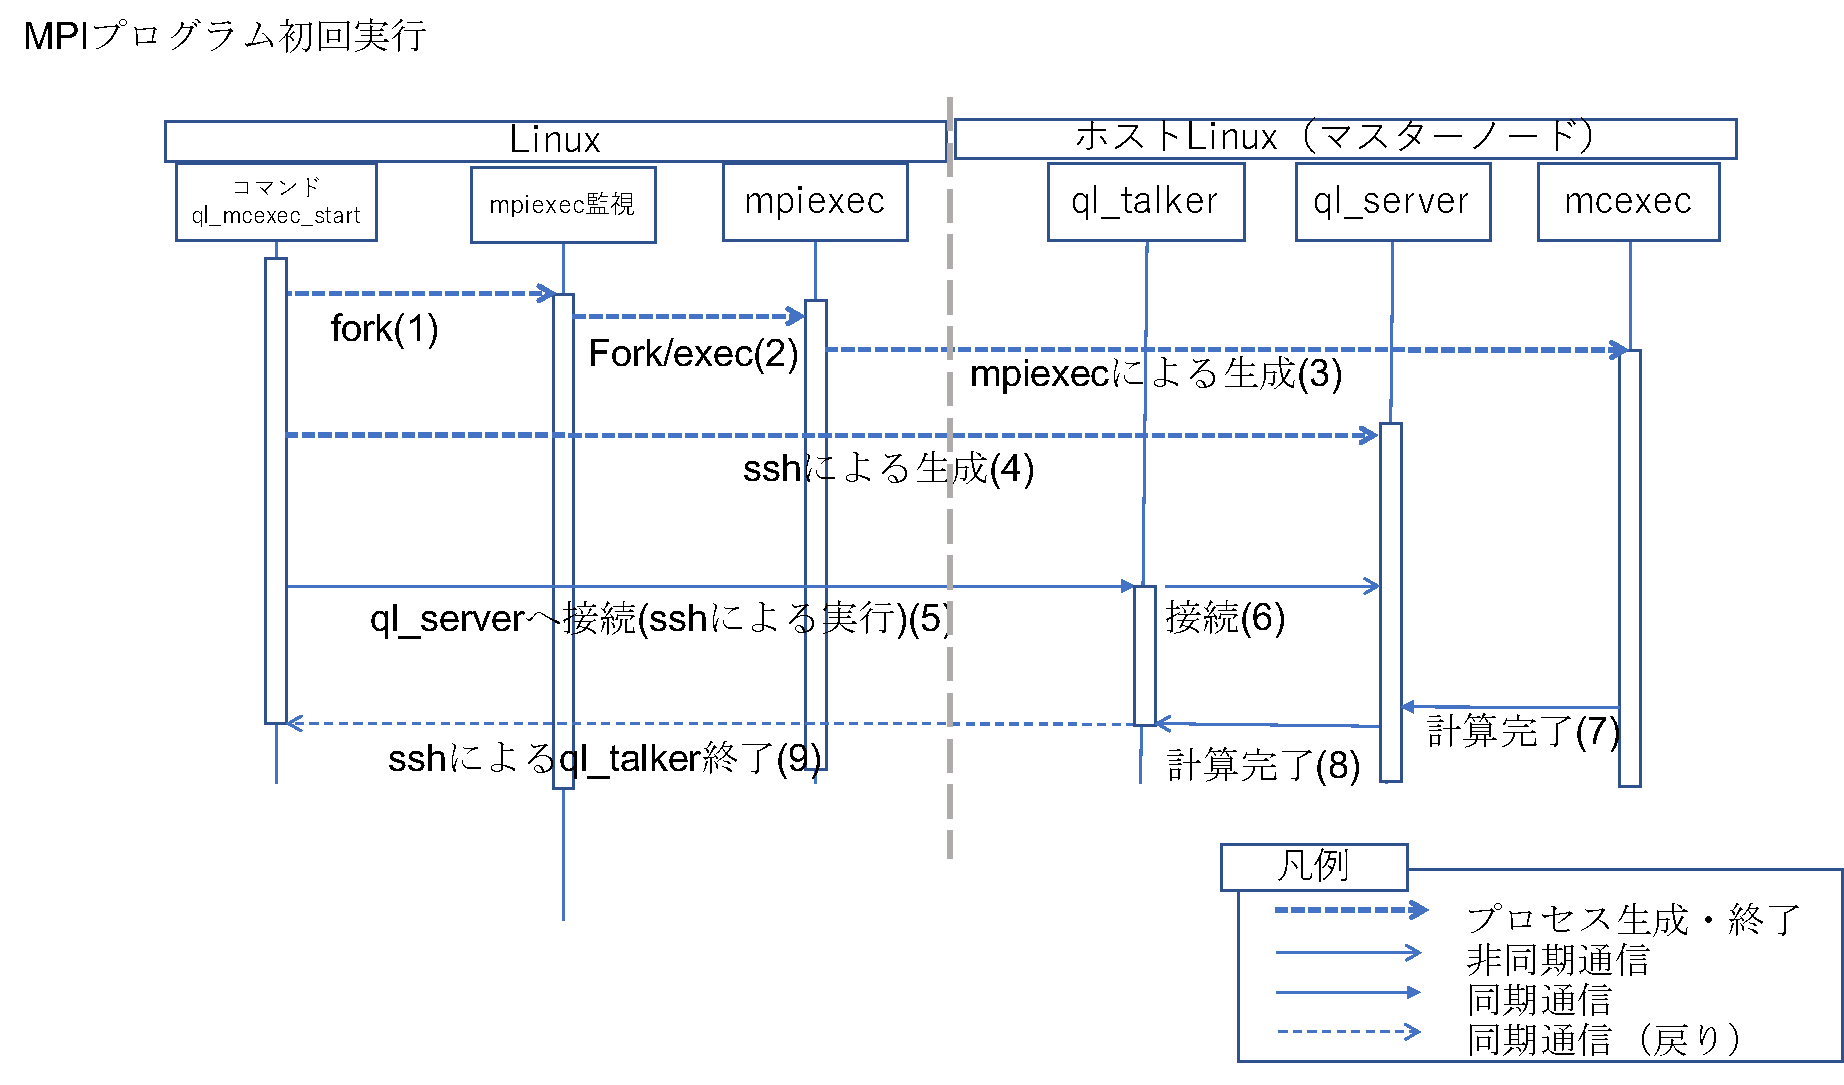
\includegraphics[width=0.90\linewidth]{figs/SequenceDiagram1.pdf}
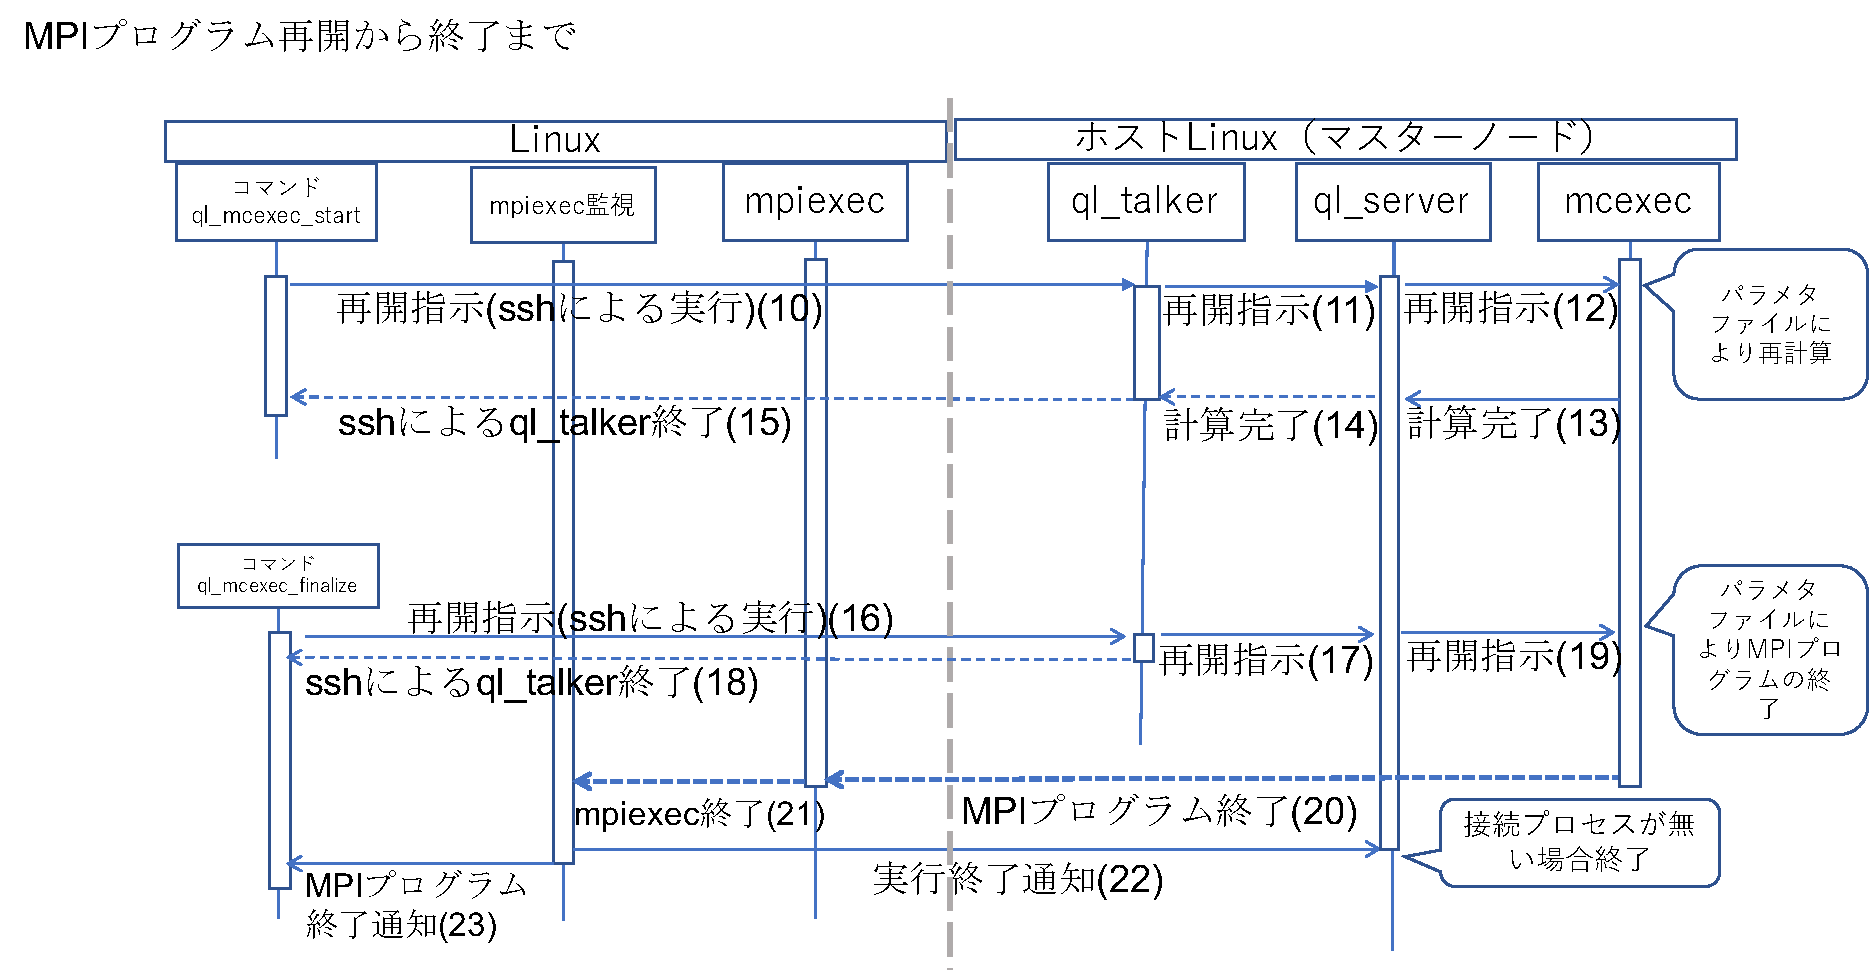
\includegraphics[width=0.90\linewidth]{figs/SequenceDiagram2.pdf}
\vspace{-0em}\caption{関連コマンドと関連プロセスの動作フロー}
\label{fig:SequenceDiagram}
\vspace{-0em}
\end{figure}
\FloatBarrier
%
\begin{itemize}
\item[01] MPIプログラムの初回実行時は、\texttt{ql\_mpiexec\_start}から、\texttt{mpiexec監視プロセス}を\texttt{fork()}で常駐プロセスとして起動する。(図の(1))
\item[02] \texttt{mpiexec監視プロセス}は、\texttt{mpiexec}を\texttt{fork()/exec()}で起動する。また、\texttt{mpiexec}の標準入出力およびエラー出力を\texttt{ql\_mpiexec\_start}へリダイレクトする。(図の(2))
\item[03] \texttt{mpiexec}が\texttt{mcexec}を用いてMPIプロセスを\texttt{McKernel}上に起動する。(図の(3))
\item[04] \texttt{ql\_mpiexec\_start}が\texttt{ssh}でホストLinux上に\texttt{ql\_server}を常駐プロセスとして起動する。(図の(4))
\item[05] \texttt{ql\_mpiexec\_start}が\texttt{ssh}でホストLinux上に\texttt{ql\_talker}を起動する。(図の(5))
\item[06] \texttt{ql\_talker}は\texttt{ql\_server}にNコマンドを送信し、\texttt{ql\_server}から計算完了の返信を待つ。\texttt{ql\_server}は当該MPIプログラムの存在を管理表に記録する。(図の(6))
\item[07] \texttt{mcexec}はMPIプログラムの一回の計算完了後
%\texttt{mckernel}がユーザプログラムのスワップアプト後、
\texttt{ql\_server}へ計算完了を意味するEコマンドを送信し、返信を待つ。(図の(7))
\item[08] \texttt{ql\_server}が \texttt{ql\_talker}へ計算完了を意味するEコマンドを送信する。(図の(8))
\item[09]  \texttt{ql\_talker}はEコマンドを受け取り、正常終了する。\texttt{ql\_mpiexec\_start}は\texttt{ql\_talker}の終了を受けてリダイレクトしている標準入出力およびエラー出力をクローズし終了する。(図の(9))
\item[10] \texttt{ql\_mpiexec\_start}はMPIプログラムの次の計算の開始時、\texttt{mpiexec監視プロセス}に依頼して\texttt{mpiexec}の標準入出力およびエラー出力を自身にリダイレクトする。また、\texttt{ssh}でホストLinux上に\texttt{ql\_talker}を起動する。(図の(10))
\item[11] \texttt{ql\_talker}は\texttt{ql\_server}へ再開指示を意味するRコマンドを送信し、\texttt{ql\_server}からの返信を待つ。(図の(11))
\item[12] \texttt{ql\_server}は\texttt{mcexec}へRコマンドを送信する。
%\texttt{mcexec}はユーザプログラムをスワップインし、
MPIプログラムはパラメタファイルを読み、再開指示であることを確認し、引数と環境変数をパラメタファイルに指定されたものに置き換え、次の回の計算を行う。(図の(12))
\item[13] \texttt{mcexec}は一回の計算完了後
%\texttt{mckernel}がユーザプログラムのスワップアプト後、
\texttt{ql\_server}へ計算完了(Eコマンド)を送信し、返信を待つ。(図の(13))
\item[14] \texttt{ql\_server}が\texttt{ql\_talker}へ計算完了(Eコマンド)を送信する。(図の(14))
\item[15]  \texttt{ql\_talker}はEコマンドを受け取り、正常終了する。\texttt{ql\_mpiexec\_start}は終了を受けてリダイレクトしている標準入出力およびエラー出力をクローズし終了する。(図の(15))
\item[16] \texttt{ql\_mpiexec\_finalize}は\texttt{mpiexec監視プロセス}に依頼して\texttt{mpiexec}の標準入出力およびエラー出力を自身へリダイレクトする。また\texttt{ssh}でホストLinux上に\texttt{ql\_talker}を起動する。(図の(16))
\item[17] \texttt{ql\_talker}は\texttt{ql\_server}へ再開指示を意味するRコマンドを送信し、終了する。(図の(17)(18))
\item[18] \texttt{ql\_server}は\texttt{mcexec}へRコマンドを送信する。
%\texttt{mcexec}はユーザプログラムをスワップインし、
MPIプロセスはRコマンドを受けて、パラメタファイルを読み終了指示であることを確認し終了処理を行う。(図の(19))
\item[19] \texttt{mcexec}はMPIプロセスの終了と共に終了する。(図の(20))
\item[20] \texttt{mpiexec}は全ランクの終了を待って終了する。\texttt{mpiexec監視プロセス}は\texttt{mpiexec}プロセス終了を検知し、戻り値を取得する。(図の(21))
\item[21] \texttt{mpiexec監視プロセス}は\texttt{ql\_talker}経由で\texttt{ql\_server}へ実行終了を意味するFコマンドを送信する。\texttt{ql\_server}は当該MPIプログラムを管理表から削除する。また、管理表が空になった場合は終了する。(図の(22))
\item[22] \texttt{mpiexec監視プロセス}は\texttt{ql\_mpiexec\_finalize}へMPIプログラムの終了を通知し、戻り値を渡し、終了する。(図の(23))
\item[23] \texttt{ql\_mpiexec\_finalize}はMPIプログラムの終了通知を受けて、リダイレクトしている標準入出力およびエラー出力をクローズし、\texttt{mpiexec}の戻り値を自身の戻り値として終了する。
\end{itemize}
\FloatBarrier

\subsection{\ADDAUGS{MPIプロセス起動指示コマンド}}
\subsubsection*{書式}{\quad} \texttt{ql\_mpiexec\_start -machinefile <hostfile\_path> {\lbrack}<mpiopts>...{\rbrack} <exe> {\lbrack}<args>...{\rbrack}}
\subsubsection*{説明}{\quad}
処理ステップは以下の通り。
\begin{itemize}
\item[1] ホストファイルの内容、\texttt{mpiexec}への引数、実行可能ファイル名からmd5ハッシュによりMPIプログラムIDを作成する。IDを環境変数\texttt{QL\_NAME}に記録する。
\item[2]\texttt{ql\_server}との通信のためのソケットファイルのパスを環境変数\texttt{QL\_SOCKET\_FILE}に記録する。また、\texttt{ssh}でホストファイルの先頭のホスト(以降、マスターノードと呼ぶ)上に\texttt{ql\_server}を起動する。起動失敗した場合は終了コード(-1)で終了する。
\item[3]  \texttt{mpiexec監視プロセス}との通信のためのソケットファイルが存在しない場合は、ソケットファイルを作成後、\texttt{mpiexec監視プロセス}を\texttt{fork}する。
%\texttt{ql\_mpiexec\_start}と\texttt{mpiexec監視プロセス}とはユニックスドメインソケットで接続する。
\texttt{mpiexec監視プロセス}は、\texttt{mpiexec}を\texttt{fork/exec}で生成する。また、\texttt{mpiexec}の標準入出力およびエラー出力を無名パイプ(以降、リダイレクト用パイプと呼ぶ)の片方の端に接続する。
\item[4]
%\texttt{mpiexec監視プロセス}と通信を行うソケットファイルが存在する場合は、
再開指示のためパラメタファイルを作成する。
\item[5]\texttt{mpiexec監視プロセス}に、自身の標準入出力、エラー出力のファイルディスクリプタ番号を渡す。\texttt{mpiexec監視プロセス}は当該ファイルディスクリプタをリダイレクト用パイプの空いている方の端に接続する。
\item[6]第1回の計算開始時は\texttt{ssh}で\texttt{ql\_talker}をマスターノード上に起動する。\texttt{ql\_talker}は、\texttt{ql\_server}へ接続を意味するNコマンドを送信し、各回の計算完了を意味するEコマンドを受信するまで待機する。
\item[7]第2回目以降の計算開始時は、\texttt{ssh}で\texttt{ql\_talker}をマスターノード上に起動する。\texttt{ql\_talker}は、\texttt{ql\_server}へ再開指示を意味するRコマンドを送信し、各回の計算完了を意味するEコマンド受信まで待機する。
\item[8] \texttt{ql\_talker}コマンドがその終了をもって\texttt{ql\_mpiexec\_start}へ計算完了を通知する。\texttt{ql\_mpiexec\_start}は\texttt{mpiexec監視プロセス}と通信を行って\texttt{mpiexec}が終了していないことを確認する。\texttt{mpiexec}が終了している場合は、\texttt{mpiexec}の終了コードを取得する。
\item[9]各回の計算完了の場合はパラメタファイルを削除し0を返し終了する。\texttt{mpiexec}が終了していた場合は、その終了コードを自身の終了コードに設定して終了する。
\end{itemize}

\texttt{ql\_mpiexec\_start}が使用する環境変数は以下の通り。
\begin{table}[!ht]
\footnotesize
\begin{tabular}{|p{0.20\linewidth}|p{0.65\linewidth}|p{0.10\linewidth}|} \hline
\multicolumn{1}{|c}{\textbf{名前}}&\multicolumn{1}{|c|}{\textbf{説明}}&\multicolumn{1}{c|}{\textbf{作成・参照}}\\ \hline 
 \hline
\texttt{QL\_NAME}&MPIプログラムID&作成\\ \hline
\texttt{QL\_SOCKET\_FILE}&\texttt{mcexec}と\texttt{ql\_server}との接続に用いるソケットファイル名&作成\\ \hline
\end{tabular}
\vspace{-0em}
\end{table}
\FloatBarrier

\texttt{ql\_mpiexec\_start}が使用するファイルは以下の通り。
\begin{table}[!ht]
\footnotesize
\begin{tabular}{|p{0.50\linewidth}|p{0.35\linewidth}|p{0.10\linewidth}|} \hline
\multicolumn{1}{|c}{\textbf{ファイル名}}&\multicolumn{1}{|c|}{\textbf{説明}}&\multicolumn{1}{c|}{\textbf{作成・参照}}\\ \hline 
 \hline
\texttt{\$\{QL\_SOCKET\_PATH\}/ql\_sock/<MPIプログラムID>.s}&\texttt{ql\_talker}と\texttt{ql\_server}との間の通信に用いるソケットファイル&作成/参照\\ \hline
\texttt{\$\{QL\_PARAM\_PATH\}/<MPIプログラムID>.param}&\texttt{ql\_mpiexec\_start}から\texttt{mcexec}への指示と、次回の計算に使用する引数と環境変数を記載するコマンド・パラメタファイル&作成\\ \hline
\end{tabular}
\vspace{-0em}
\end{table}
\FloatBarrier

パラメタファイルは、\texttt{ql\_mpiexec\_\{start,finalize\}}から\texttt{mcexec}への指示を記載する。
内容は、起床後の動作および次の回の計算に必要な引数などのデータである。

フォーマットは以下の通り。
\begin{verbatim}
<ヘッダ部>
<データ部>
[<データ部>...]
\end{verbatim}

\texttt{<ヘッダ部>}のフォーマットは以下の通り。
\begin{verbatim}
0 COM=<mcexecへの指示> <引数の数> <環境変数定義の数>
\end{verbatim}
%
それぞれのフィールドの意味及び取りうる値は以下の通り。
\begin{table}[!ht]
\footnotesize
\begin{tabular}{|p{0.20\linewidth}|p{0.75\linewidth}|} \hline
\multicolumn{1}{|c}{\textbf{フィールド}}&\multicolumn{1}{|c|}{\textbf{説明}}\\ \hline \hline
\texttt{<mcexecへの指示>}&R:次の回の計算開始、F:MPIプロセスの終了\\ \hline
\texttt{<引数の数>}&データ部に存在する引数の数\\ \hline
\texttt{<環境変数定義の数>}&データ部に存在する環境変数定義の数\\ \hline
\end{tabular}
\vspace{-0em}
\end{table}

\texttt{<データ部>}のフォーマットは以下の通り。
\begin{verbatim}
<種別> <データ長> <データ値>
\end{verbatim}
それぞれのフィールドの意味及び取りうる値は以下の通り。
\begin{table}[!ht]
\footnotesize
\begin{tabular}{|p{0.20\linewidth}|p{0.75\linewidth}|} \hline
\multicolumn{1}{|c}{\textbf{フィールド}}&\multicolumn{1}{|c|}{\textbf{説明}}\\ \hline \hline
\texttt{<種別>}&1:引数、2:環境変数定義\\ \hline
\texttt{<データ長>}&データ長\\ \hline
\texttt{<データ値>}&文字列\\ \hline
\end{tabular}
\vspace{-0em}
\end{table}

\subsection{\ADDAUGS{MPIプロセス終了指示コマンド}}
\subsubsection*{書式}{\quad} \texttt{ql\_mpiexec\_finalize -machinefile <hostfile> {\lbrack}<mpiopts>...{\rbrack}  <exe> }
\subsubsection*{説明}{\quad}
処理ステップは以下の通り。
\begin{itemize}
\item[1] ホストファイルの内容、\texttt{mpiexec}への引数、実行可能ファイル名からmd5ハッシュによりMPIプログラムIDを作成し、環境変数\texttt{QL\_NAME}に記録する。
\item[2]  \texttt{mpiexec監視プロセス}と通信を行うソケットファイルの存在を確認し、存在しない場合は\texttt{ql\_mpiexec\_start}が実行されていないと判断し1を返し終了する。
\item[3]終了指示のためのパラメタファイルを作成する。
\item[4]\texttt{ql\_mpiexec\_finalize}は自身の標準入出力とエラー出力のファイルディスクリプタ番号を\texttt{mpiexec監視プロセス}に渡す。\texttt{mpiexec監視プロセス}は当該ファイルディスクリプタをリダイレクト用パイプの空いている方の端に接続する。
\item[5]\texttt{ssh}でマスターノード上に\texttt{ql\_talker}を起動する。\texttt{ql\_talker}は、\texttt{ql\_server}へ再開指示を意味するRコマンドを送信する。\texttt{ql\_mpiexec\_start}の場合と異なり\texttt{ql\_talker}は\texttt{ql\_server}からの返答を待つことなく終了する。
\item[6] \texttt{mpiexec監視プロセス}は\texttt{mpiexec}の終了時にその終了コードを自身の終了コードに設定し終了する。
\item[7] \texttt{mpiexec監視プロセス}の終了を受けてパラメタファイルを削除する。また\texttt{mpiexec監視プロセス}から渡された\texttt{mpiexec}の終了コードを自身の終了コードに設定して終了する。
\end{itemize}

\texttt{ql\_mpiexec\_finalize}で作成/参照する環境変数は以下の通り。
\begin{table}[!ht]
\footnotesize
\begin{tabular}{|p{0.15\linewidth}|p{0.60\linewidth}|p{0.15\linewidth}|} \hline
\multicolumn{1}{|c}{\textbf{名前}}&\multicolumn{1}{|c|}{\textbf{説明}}&\multicolumn{1}{c|}{\textbf{作成・参照}}\\ \hline 
 \hline
\texttt{QL\_NAME}&MPIプログラムID&作成\\ \hline
\end{tabular}
\vspace{-0em}
\end{table}
\FloatBarrier

\texttt{ql\_mpiexec\_finalize}で作成/参照するファイルは以下の通り。
\begin{table}[!ht]
\footnotesize
\begin{tabular}{|p{0.50\linewidth}|p{0.35\linewidth}|p{0.10\linewidth}|} \hline
\multicolumn{1}{|c}{\textbf{ファイル名}}&\multicolumn{1}{|c|}{\textbf{説明}}&\multicolumn{1}{c|}{\textbf{作成・参照}}\\ \hline 
 \hline
\texttt{\$\{QL\_SOCKET\_PATH\}/ql\_sock/<MPIプログラムID>.s}&\texttt{ql\_talker}と\texttt{ql\_server}との間の通信に用いるソケットファイル&参照\\ \hline
\texttt{\$\{QL\_PARAM\_PATH\}/<MPIプログラムID>.param}&\texttt{ql\_mpiexec\_finalize}から\texttt{mcexec}への指示を記載するコマンドファイル。&作成\\ \hline
\end{tabular}
\vspace{-0em}
\end{table}
\FloatBarrier

\subsection{\ADDAUGS{MPI実行環境初期化関数(C言語)}}
\subsubsection*{書式}{\quad} \texttt{int MPI\_Init(int *argc,char ***argv)}
\comment{
\subsubsection*{引数}{\quad}
\begin{table}[!ht]
\footnotesize
\begin{tabular}{|p{0.15\linewidth}|p{0.75\linewidth}|} \hline
\multicolumn{1}{|c}{\textbf{引数}}&\multicolumn{1}{|c|}{\textbf{説明}}\\ \hline \hline
\texttt{argc}&引数の数へのポインタ\\ \hline
\texttt{argv}&引数文字列の配列へのポインタ\\ \hline
\end{tabular}
\vspace{-0em}
\end{table}
}
\subsubsection*{説明}{\quad}
\texttt{argc, argv}を用いて高速プロセス起動の初期化を行う。
本関数はPMPIインタフェースにより\texttt{MPI\_Init()}を置き換える。

処理のステップは以下の通り。
\begin{itemize}
\item[1]\texttt{PMPI\_init()}関数を呼び出し、MPI環境を初期化する。また、引数情報を取得する。
\item[2]\texttt{PMPI\_init()}が正常終了した場合、\texttt{ql\_init()}関数を呼び出し、高速プロセス起動を初期化する。
\item[3]\texttt{PMPI\_init()}の戻り値自身の戻り値に設定して戻る。
\end{itemize}

\subsubsection*{戻り値}{\quad}
\begin{table}[!ht]
\footnotesize
\begin{tabular}{|p{0.15\linewidth}|p{0.75\linewidth}|} \hline
\multicolumn{1}{|c}{\textbf{戻り値}}&\multicolumn{1}{|c|}{\textbf{説明}}\\ \hline \hline
\texttt{MPI\_SUCCESS}&正常終了\\ \hline
\texttt{MPI\_ERR\_OTHER}&\texttt{MPI\_init()}が複数回実行された\\ \hline
\end{tabular}
\vspace{-0em}
\end{table}
\FloatBarrier

\subsection{\ADDAUGS{MPI実行環境初期化関数(fortran)}}
\subsubsection*{書式}{\quad} \texttt{subroutine MPI\_INIT(INT ierr)}
\comment{
\subsubsection*{引数}{\quad}
\begin{table}[!ht]
\footnotesize
\begin{tabular}{|p{0.15\linewidth}|p{0.75\linewidth}|} \hline
\multicolumn{1}{|c}{\textbf{引数}}&\multicolumn{1}{|c|}{\textbf{説明}}\\ \hline \hline
\texttt{ierr}&戻り値\\ \hline
\end{tabular}
\vspace{-0em}
\end{table}
\FloatBarrier
}
\subsubsection*{説明}
Fortran環境において、高速プロセス起動のための初期化を行う。本関数は、PMPIインタフェースにより\texttt{MPI\_INIT}を置き換えることで実装される。
%
処理のステップは以下の通り。
\begin{itemize}
\item[1]\texttt{pmpi\_init\_()}が存在していない場合、\texttt{ierr}に\texttt{MPI\_ERR\_OTHER}をセットして戻る。
\item[2]\texttt{pmpi\_init\_()}を呼び出し、MPI環境を初期化する。
\item[3]戻り値\texttt{ierr}が\texttt{MPI\_SUCCESS}の場合、\texttt{ql\_init()}関数を呼び出し、高速プロセス起動を初期化する。
\end{itemize}

なお、FortranコンパイラはGNU Fortran CompilerもしくはIntel Fortran Compilerをサポートする。Intel Fortran Compilerを使用する場合は、コンパイルオプションに-shared-intelを指定する必要がある。

\subsubsection*{戻り値}{\quad}
\begin{table}[!ht]
\footnotesize
\begin{tabular}{|p{0.15\linewidth}|p{0.75\linewidth}|} \hline
\multicolumn{1}{|c}{\textbf{戻り値}}&\multicolumn{1}{|c|}{\textbf{説明}}\\ \hline \hline
\texttt{MPI\_SUCCESS}&正常終了\\ \hline
\texttt{MPI\_ERR\_OTHER}&\texttt{MPI\_init()}が複数回実行された\\ \hline
\end{tabular}
\vspace{-0em}
\end{table}
\FloatBarrier

\subsection{\ADDAUGS{計算の再開・終了関数(C言語)}}
\subsubsection*{書式}{\quad} \texttt{ql\_client(int *argc,char ***argv)}
\subsubsection*{説明}{\quad}
処理のステップは以下の通り。
\begin{itemize}
\item[1]当該プロセスが\texttt{ql\_mpiexec\_start}により起動されていない場合は、\texttt{QL\_EXIT}を返す。
\item[2]スレッドの停止を行う。また\texttt{PMI\_Barrier()}で計算完了同期を行う。
\item[3]
%スワップアウトシステムコールを呼び出し、
システムコールによりカーネルモードに移行し、\texttt{mcexec}に
%スワップ完了同期及び
\texttt{ql\_mpiexec\_\{start,finalize\}}による指示待ちを依頼する。
\item[4]指示待ちから復帰し、パラメタファイルを参照して指示を確認する。指示が次の回の計算開始の場合、パラメタファイルを用いて計算のための引数と環境変数を設定する。
\item[5] スレッドの再開を行う。
\item[6] 指示が次の回の計算開始の場合\texttt{QL\_CONTINUE}、MPIプロセスの終了の場合\texttt{QL\_EXIT}を返す。
\end{itemize}

\subsection{\ADDAUGS{計算の再開・終了関数(Fortran)}}
\subsubsection*{書式}{\quad} \texttt{subroutine QL\_CLIENT(ierr)}
\subsubsection*{説明}
\texttt{ql\_client()}を呼び、その戻り値を\texttt{ierr}に格納して戻る。

\subsection{\ADDAUGS{初期化関数}}
\subsubsection*{書式}{\quad} \texttt{int ql\_init(int argc, char **argv)}
\subsubsection*{説明}{\quad}
\texttt{MPI\_Init()}から呼びされ、高速プロセス起動の初期化を行う。

処理ステップは以下の通り。
\begin{itemize}
\item[1]環境変数\texttt{QL\_NAME}からMPIプログラムIDを取得する。
取得できなかった場合、\texttt{ql\_mpiexec\_start}から起動されていないと判断し、\texttt{QL\_NORMAL}を返す。
\item[3]MPIプログラムIDから、パラメタファイルのパス
%とスワップファイルパス
を作成する。
%スワップファイルパスはMPプログラムIDに自プロセスの\texttt{RANK}を加えたファイル名とすることで、ランク毎に一意な名称とする。
\item[4]\texttt{QL\_SUCCESS}を返す。
\end{itemize}
\FloatBarrier

\subsubsection*{戻り値}{\quad}
\begin{table}[!ht]
\footnotesize
\begin{tabular}{|p{0.15\linewidth}|p{0.75\linewidth}|} \hline
\multicolumn{1}{|c}{\textbf{戻り値}}&\multicolumn{1}{|c|}{\textbf{説明}}\\ \hline \hline
\texttt{QL\_SUCCESS}&高速プロセス起動の初期化成功\\ \hline
\texttt{QL\_NORMAL}&当該プロセスが\texttt{ql\_mpiexec\_start}から起動されていない\\ \hline
\end{tabular}
\vspace{-0em}
\end{table}
\FloatBarrier

\subsection{\ADDAUGS{計算ノードの管理サーバ}}
\subsubsection*{書式}{\quad} \texttt{ql\_server}
\subsubsection*{説明}{\quad}
\texttt{ql\_server}は、\texttt{ql\_mpiexec\_start}により\texttt{RANK\#0}が存在する計算ノード上に起動され、以下の処理を行う。
%
\begin{itemize}
\item[1]既に\texttt{ql\_server}が起動されている場合は、-1を返して終了する。
\item[2]\texttt{mcexec}、\texttt{ql\_talker}との通信に用いるユニックスドメインソケットをオープンする。
\item[3]\texttt{select()}で当該ソケットを監視する。
\item[4]電文を読み込み、コマンドとデータを取得する。
\item[5]\texttt{ql\_talker}からNコマンドを受け取った際は、対応するMPIプログラムを管理表に登録する。また、MPIプロセスIDをインデックスとし\texttt{ql\_server}に接続しているプロセスを返すマップ(接続マップと呼ぶ)に\texttt{ql\_talker}を登録する。\\
接続マップは\texttt{struct client\_fd}で実装される。
\texttt{struct client\_fd}は以下のように定義される。
\begin{verbatim}
struct client_fd {
        int fd;         // 接続元プロセスのファイルディスクリプタ
        int client;     // 接続元プロセスの種別
        char *name;     // MPIプログラムID
        int status;     // 現在実行中の通信コマンド
};
\end{verbatim}

\item[6]\texttt{mcexec}からEコマンドを受けとった際は、\texttt{ql\_mpiexec\_\{start,finalize\}}の指示があるまで待たせる。また、\texttt{mcexec}を接続マップに登録する。さらに、接続マップを用いて対応する\texttt{ql\_talker}を見つけ、それに対してEコマンドを送信する。
\item[7]\texttt{ql\_talker}からRコマンドを受けとった際は、\texttt{ql\_talker}を接続マップに登録する。また、接続マップを用いて対応する\texttt{mcexec}プロセスを見つけ、それに対してRコマンドを送信することで\texttt{mcexec}を起床する。
\item[8]\texttt{mpiexec監視プロセス}からFコマンドを受け取った際は、対応するMPIプログラムを管理表から削除する。管理表が空になった場合は\texttt{ql\_server}自身も終了する。
\end{itemize}

\texttt{ql\_talker}や\texttt{mcexec}が\texttt{ql\_server}と通信するために使用するソケットファイルは、環境変数\texttt{QL\_SOCKET\_PATH}が定義されている場合は\texttt{\$\{QL\_SOCKET\_PATH\}/ql\_sock}下に、定義されていない場合は\texttt{/run/user/ユーザID/ql\_sock}下に作成される。当該ディレクトリは\texttt{ql\_mpiexec\_start}コマンドが実行されるノードとランク\texttt{\#0}が実行されるノードからアクセスできる必要がある。

\subsection{\ADDAUGS{指示中継コマンド}}
\subsubsection*{書式}{\quad} \texttt{ql\_talker <send\_command> <receive\_command> <MPI\_Program\_ID>}
\subsubsection*{引数}{\quad}
\begin{table}[!ht]
\footnotesize
\begin{tabular}{|p{0.20\linewidth}|p{0.75\linewidth}|} \hline
\multicolumn{1}{|c}{\textbf{引数}}&\multicolumn{1}{|c|}{\textbf{説明}}\\ \hline \hline
\texttt{<send\_command>}&\texttt{ql\_server}へ送信するコマンド(1文字)を指定する。\\ \hline
\texttt{<receive\_command>}&\texttt{ql\_server}からの受信を期待するコマンド(1文字)を指定する。受信を待たずに終了する場合は、''\texttt{-n}''を指定する。\\ \hline
\texttt{<MPI\_Program\_ID>}&MPIプログラムIDを指定する。\\ \hline
\end{tabular}
\vspace{-0em}
\end{table}
\FloatBarrier

\subsubsection*{説明}{\quad}
\texttt{ql\_mpiexec\_\{start,finalize\}}から\texttt{ql\_server}が動作するノード上に起動され、\texttt{ql\_server}に\texttt{<send\_command>}で指定されたコマンドを送り、\texttt{<receive\_command>}で指定された応答を待つ。
\texttt{ql\_server}とはユニックスドメインソケットを用いて通信する。

処理ステップは以下の通り。
\begin{itemize}
\item[1]\texttt{argc}の数をチェックし、4未満の場合は終了コード-1 で終了する。
\item[2]環境変数を参照して\texttt{ql\_server}との接続に用いるユニックスドメインソケットを見つけ、\texttt{ql\_server}に接続する。
\item[3]\texttt{<send\_command>}と\texttt{<MPI\_Program\_ID>}より電文を作成し、\texttt{ql\_server}へ電文を送信する。失敗した場合は終了コード-1で終了する。
\item[4]\texttt{<receive\_command>}に"-n"が指定されていた場合、終了コード0で終了する。
\item[5]\texttt{<receive\_command>}を受信した場合、終了コード0で終了する。
%ソケット通信が失敗した場合、終了コード-1
\texttt{<receive\_command>}以外の文字列を受信した場合終了コード-2で終了する。
\end{itemize}

\subsubsection*{戻り値}{\quad}
\begin{table}[!h]
\footnotesize
\begin{tabular}{|p{0.15\linewidth}|p{0.75\linewidth}|} \hline
\multicolumn{1}{|c}{\textbf{戻り値}}&\multicolumn{1}{|c|}{\textbf{説明}}\\ \hline \hline
\texttt{0}&正常終了\\ \hline
\texttt{-1}&ソケット通信エラー\\ \hline
\texttt{-2}&\texttt{<receive\_command>}以外の文字列を受信\\ \hline
\end{tabular}
\vspace{-0em}
\end{table}
\FloatBarrier

\subsection{\MODMARS{\texttt{swapout}システムコール}}
\subsubsection*{書式}{\quad} \texttt{int swapout(char *filename, void *workarea, size\_t size, int flag)}
\subsubsection*{引数}{\quad}
\begin{table}[!ht]
\footnotesize
\begin{tabular}{|p{0.15\linewidth}|p{0.75\linewidth}|} \hline
\multicolumn{1}{|c}{\textbf{引数}}&\multicolumn{1}{|c|}{\textbf{説明}}\\ \hline \hline
\texttt{filename}&スワップファイル名へのポインタ\\ \hline
\texttt{workarea}&作業領域へのポインタ\\ \hline
\texttt{size}&作業領域のサイズ\\ \hline
\texttt{flag}&swapoutの動作制御用フラグ \\ \hline
\end{tabular}
\vspace{-0em}
\end{table}

\subsubsection*{説明}{\quad}
\subsubsection*{A. スワップアウト処理}{\quad}\\
%
\begin{figure}[!h]
\centering
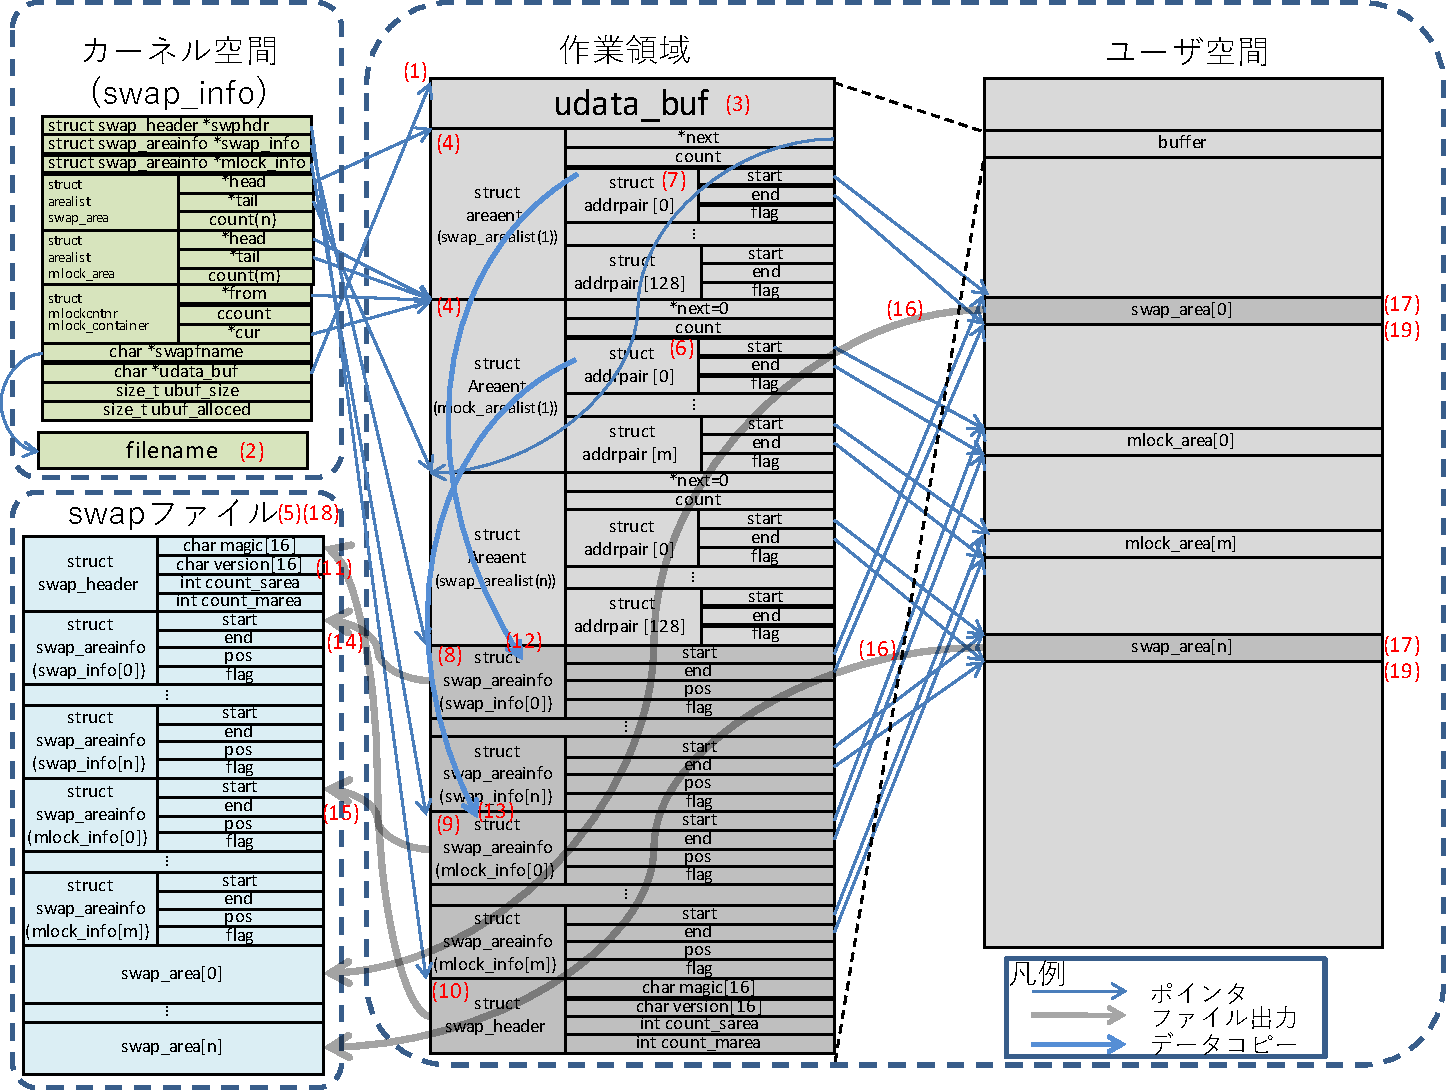
\includegraphics[width=0.90\linewidth]{figs/pageout.pdf}
\vspace{-0em}\caption{スワップアウトの処理フロー}
\label{fig:pageout}
\vspace{-0em}
\end{figure}
\FloatBarrier
%
スワップアウトの処理フローを図\ref{fig:pageout}を用いて説明する。
\begin{enumerate}
\item McKernelのユーザから渡された作業領域を\texttt{mlock()}によりロックする。swapout情報を管理する\texttt{swap\_info}構造体の\texttt{udata\_buf}メンバに作業領域の先頭アドレスを記録する。 (図の(1))
\item 引数で指定されたファイル名を\texttt{copy\_from\_user}でカーネル空間にコピーする。\texttt{swap\_info}構造体の\texttt{swapfname}メンバにファイル名のアドレスを記録する。 (図の(2))
\item 作業領域に汎用バッファ\texttt{udata\_buf}を割り当てる。 (図の(3))
\item 作業領域にスワップエリア管理用リスト\texttt{swap\_arealist}と\texttt{mlock}エリア管理用リスト\texttt{mlock\_arealist}の領域を割り当てる。 (図の(4))
\item swapファイルを\texttt{open()}でオープンする。 (図の(5))
\item \texttt{lookup\_process\_memory\_range}および\texttt{next\_process\_memory\_range}を用いて、ユーザプロセスのメモリ領域を検索し、それぞれについて以下を行う。
\begin{enumerate}
\item \texttt{mlock()}されている領域の開始アドレス、終了アドレス、flagを作業領域の\textttw{mlock\_arealist}に記録する。 (図の(6))
\item \texttt{mlock()}されていない領域の開始アドレス、終了アドレス、flagを作業領域の\texttt{swap\_arealist}に記録する。 (図の(7))
\end{enumerate}
\item 作業領域の\texttt{swap\_arealist}のエントリ数と同数のエントリを持つ\texttt{swap\_info}配列を作業領域に割り当てる。カーネル領域の\texttt{swap\_info}構造体の\texttt{swap\_info}メンバに作業領域の\texttt{swap\_info}配列の先頭アドレスを記録する。 (図の(8))
\item 作業領域の\texttt{mlock\_arealist}のエントリ数と同数のエントリを持つ\texttt{mlock\_info}配列を作業領域に割り当てる。カーネル領域の\texttt{swap\_info}構造体の\texttt{mlock\_info}メンバに作業領域の\texttt{mlock\_info}配列の先頭アドレスを記録する。 (図の(9))
\item 作業領域に\texttt{swap\_header}を割り当てる。カーネル領域の\texttt{swap\_info}構造体の\texttt{swphdr}メンバに先頭アドレスを記録する。 (図の(10))
\item 作業領域の\texttt{swap\_header}の\texttt{magic}メンバに"McKernel swap"、versionメンバに"0.9.0"、\texttt{count\_sarea}メンバに\texttt{swap\_arealist}のエントリ数、\texttt{count\_marea}メンバに\textttw{mlock\_arealist}のエントリ数を記録する。
\item 作業領域の\texttt{swap\_header}を\texttt{write()}を用いてスワップファイルへ書き出す。 (図の(11))
\item 作業領域の\texttt{swap\_arealist}のリスト形式データを作業領域の\texttt{swap\_info}配列へコピーする。 (図の(12))
\item 作業領域の\texttt{mlock\_arealist}のリスト形式データを作業領域の\texttt{mlock\_info}配列へコピーする。 (図の(13))
\item 作業領域の\texttt{swap\_info}配列を\texttt{write()}を用いてスワップファイルへ書き出す。 (図の(14))
\item 作業領域の\texttt{mlock\_info}配列を\texttt{write()}を用いてスワップファイルへ書き出す。 (図の(15))
\item 作業領域の\texttt{swap\_info}の情報を用いて、ユーザプロセスのメモリ領域のうち、スワップアウト対象となっているものを\texttt{write()}を用いてスワップファイルへ出力する。 (図の(16))
\item スワップアウト対象となっているメモリ領域のうち、McKernel側でマップされているものを\texttt{ihk\_mc\_pt\_free\_range()}でアンマップする。 (図の(17))
\item スワップファイルを\texttt{close()}を用いてクローズする。 (図の(18))
\item スワップアウト対象となっているメモリ領域のうち、Linux側でマップされているものを\texttt{mcexec}に依頼することでアンマップする。 (図の(19))
\end{enumerate}

\subsubsection*{B. スワップイン処理}{\quad}\\
%
\begin{figure}[!h]
\centering
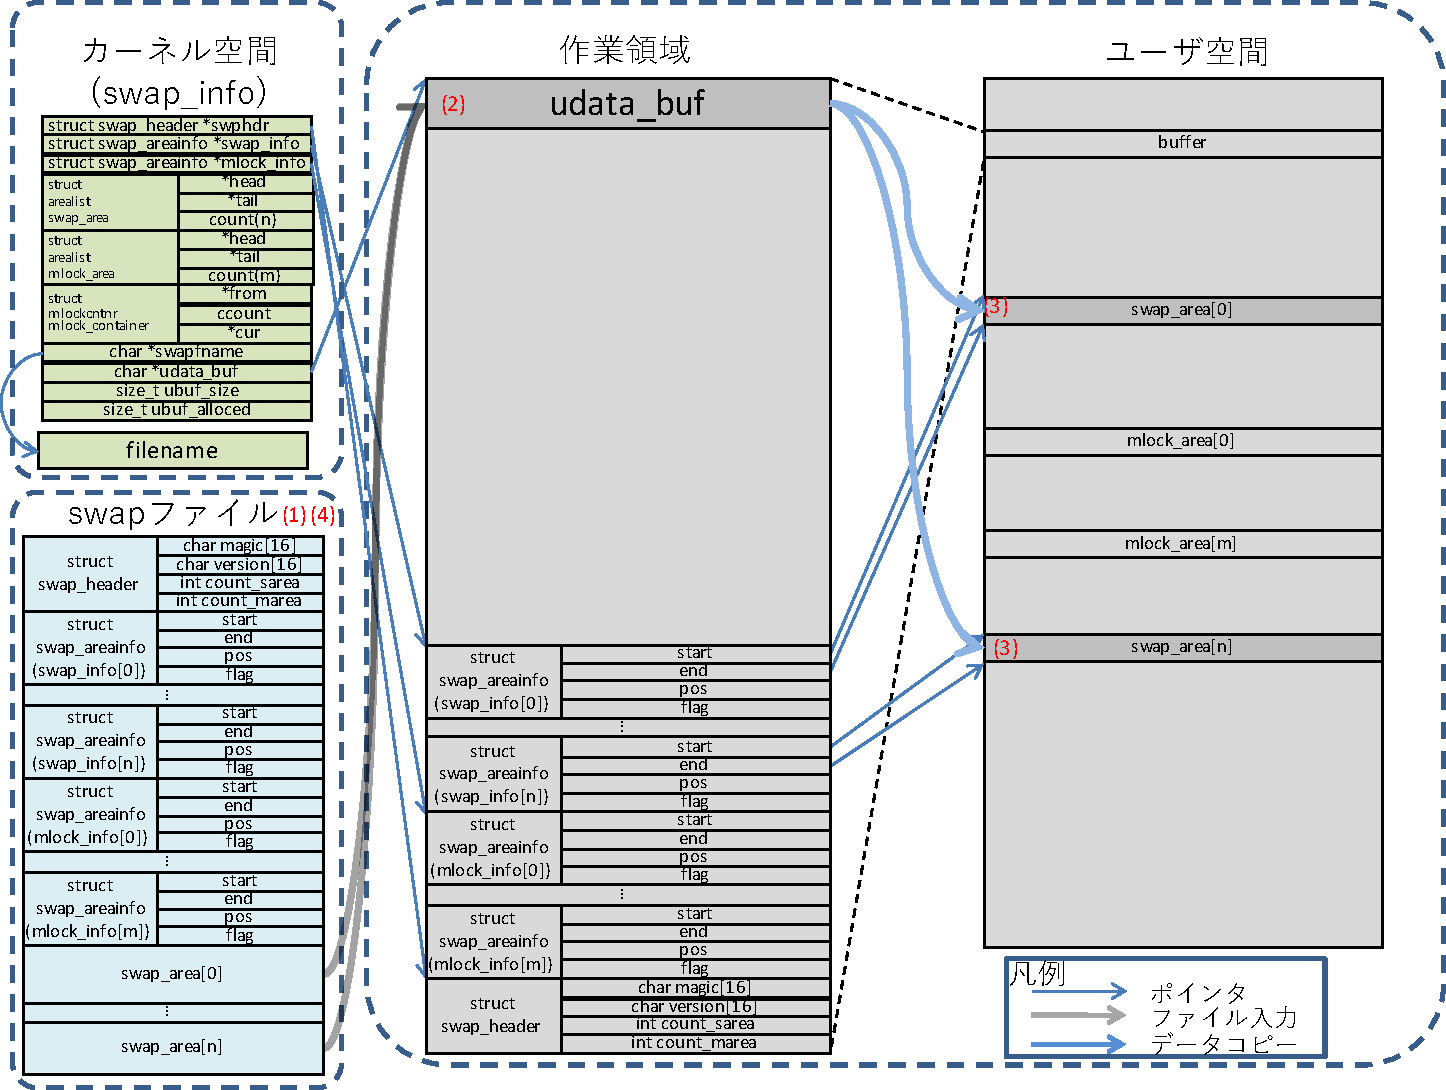
\includegraphics[width=0.90\linewidth]{figs/pagein.pdf}
\vspace{-0em}\caption{スワップインの処理フロー}
\label{fig:pagein}
\vspace{-0em}
\end{figure}
\FloatBarrier
%
スワップインの処理フローを図\ref{fig:pagein}を用いて説明する。
\begin{enumerate}
\item スワップファイルを\texttt{open()}を用いてオープンする。 (図の(1))
\item スワップイン対象アドレス範囲を記録している\texttt{swap\_info}配列の各エントリに対して以下を行う。なお、ユーザ空間の作業領域はスワップアウトを経ても残っているため、\texttt{swap\_info}配列をファイルから取得する必要はない。
\begin{enumerate}
\item \texttt{read()}を用いてスワップファイルから作業領域の\texttt{udata\_buf}へスワップイン対象のメモリ内容をコピーする。 (図の(2))
\item \texttt{copy\_to\_user}を用いて、作業領域の\texttt{udata\_buf}からユーザプロセスのメモリ領域へ、スワップイン対象のメモリ内容をコピーする。 (図の(3))
\end{enumerate}
\item スワップファイルを\texttt{close()}を用いてクローズする。 (図の(4))
\end{enumerate}
\FloatBarrier

\section{Portability}

IHK/McKernel has been designed not only for post K computer but also
for other manycore architectures, including Intel Xeon phi.
In order to make the source code portable as much as possible.
The following is coding convention of IHK/McKernel.

The directories for architecture dependent and indepent source codes are
created and codes are separately stored into those two directories.
That is, source codes, including header files, for some specific
architecture are located in its architecture dependent directory.

The source codes, accessing some hardware registers, are hardware
specific, and thus those are machine dependent.  Low-level interrupt
handlers, some memory management codes, context switch codes, and
signaling codes are the examples. Those source codes are located in an
architecture dependent directory.

Any program code and header files must not include any machine
dependent codes including conditional compile macros, such as
\verb+#ifdef ARCH+.
As much as possible, we define machine independent interfaces so that
those interfaces are implemented for each architecture.

\section{Formal Verification}

Some of the behaviors of McKernel is verified in a formal way by embedding behaviors in code and running a verification engine.
% For example, it is verified that no blocking code is executed while disabling IRQ.
We employ an extented version of the ANSI/ISO C Specification Language,
whose extensions\cite{pbus} were developed at the project ``Dependable Operating
Systems for Embedded Systems Aiming at Practical Applications'' in the
research area named Core Research for Evolutional Science and
Technology (CREST), sponsored by Japan Science and Technology Agency
(JST).

%=============================================================================
\subsection{Specification Language}
%=============================================================================
The following are expressions defined in the formal specification language.
The behavior of each function is formally specified by using those
expressions that are written as C comments.

\begin{description}
\item[\texttt{{\textbackslash}result}] specifys return vaule.
\item[\texttt{{\textbackslash}interrupt\_disabled}]
the CPU is interruptable if 0,
the CPUr is not interruptable if 1 or more.
\item[\texttt{{\textbackslash}process\_env}] 
the execution is under the user context if 1 or more,
the execution is under the kernel context if 0.
\item[\texttt{{\textbackslash}atomicity}] 
the execution is not allowed to block if 1 or more,
the execution may be suspended if 0.
\item[\texttt{{\textbackslash}dont\_call\_schedule}] 
the context switch is not allowed if 1 or more,
the context switch is allowed if 0.
\item[\texttt{is\_locked($\langle$pointer variable$\rangle$)}]
returns true if a memory block pointed by the pointer variable is the
lock status, otherwise
returns false.
\item[\texttt{requires} $\langle$condition expression$\rangle$]
The condition expression must be satisfied at the begining of the function
execution.
\item[\texttt{ensures} $\langle$condition expression$\rangle$]
The condition expression must be satisfied at the end of the function
execution.
\item[\texttt{invariant} $\langle$condition expression$\rangle$] 
The condition expression must be satisfied during the function execution.
\end{description}

Here is a sample code.
\begin{verbatim}
/*@
  @ behavior valid_vector:
  @   assumes 32 <= vector <= 255;
  @   requires \valid(h);
  @   assigns handlers[vector-32];
  @   ensures \result == 0;
  @ behavior invalid_vector:
  @   assumes (vector < 32) || (255 < vector);
  @   assigns \nothing;
  @   ensures \result == -EINVAL;
  @*/
int ihk_mc_register_interrupt_handler(int vector,
                                      struct ihk_mc_interrupt_handler *h)
{
    if (vector < 32 || vector > 255) {
      return -EINVAL;
    }
    list_add_tail(&h->list, &handlers[vector - 32]);
    return 0;
}
\end{verbatim}

\comment{
%=============================================================================
\subsection{記述するソースコードの範囲}
%=============================================================================
また、記述するソースコードの範囲は、以下の2つとする。
\begin{enumerate}
\item アーキ非依存部とアーキ依存部の境目のインターフェイス宣言部
\item アノテーションによって動作がわかりやすくなる以下の関数
\begin{description}
\item[\texttt{alloc\_pages}] 引数によってエラー時の対処法の切り替えがあるため
\end{description}
\end{enumerate}
}

%=============================================================================
\section{\MODMARS{Limitations}}
%=============================================================================
\MODMAR{Certain system calls are only partially implemented in McKernel or not conforming Linux API.}
These are either due to design restrictions of the proxy approach
or because their support is intentionally omitted. 
Table \ref{tab:sclim} shows the limitations.

\begin{table}[!htb]
\centering
\footnotesize
\caption{Limitations of McKernel}\vspace{0.0em}
\label{tab:sclim}
\begin{tabular}{|p{0.20\linewidth}|p{0.75\linewidth}|} \hline
\multicolumn{1}{|c}{\textbf{Function}}&\multicolumn{1}{|c|}{\textbf{Description}}\\ \hline \hline
\texttt{arch\_prctl}&It returns the \texttt{EOPNOTSUPP} error when \texttt{ARCH\_SET\_GS} is passed.\\ \hline
\texttt{brk}&It extends the heap more than requestd when \texttt{-h (--extend-heap-by=)<step>} option of \texttt{mcexec} is used with the value larger than 4~KiB.\\ \hline
\texttt{clone}&\begin{tabular}[t]{@{}l@{}}
It supports only the following flags. All other flags cause clone() to return error \\
or are simply ignored.\\
\textbullet~~\texttt{CLONE\_CHILD\_CLEARTID}\\
\textbullet~~\texttt{CLONE\_CHILD\_SETTID}\\
\textbullet~~\texttt{CLONE\_PARENT\_SETTID}\\
\textbullet~~\texttt{CLONE\_SETTLS}\\
\textbullet~~\texttt{CLONE\_SIGHAND}\\
\textbullet~~\texttt{CLONE\_VM}\\
\end{tabular}
\comment{The combination of \texttt{CLONE\_VM} flag set and \texttt{CLONE\_THREAD} flag unset is not supported. This is because this combination is rarely used in the applications.
%
The Linux side must track a thread group information for a new thread which is created with this combination of flags.
This is because the flag combination means the new thread has its own thread group and the Linux side need to track the information as the Linux side needs to handle thread group related operations.
For example, when the new thread calls \texttt{exit\_group()}, the Linux side sends signals to members of the thread group of the calling thread and the Linux side must refer to the information to do so.
%
But this requirement conflicts with the design decision where the Linux side does not track the information (by making \texttt{mcexec} invoke \texttt{clone()}) when threads are created to reduce the overhead of \texttt{clone()}.}
\\ \hline
\ADDMAR{\texttt{getrusage}}&\ADDMAR{The time spent is measured in a different way than Linux for \texttt{RUSAGE\_THREAD}. That is, time spent in user-mode and kernel-mode are updated when CPU mode changes (i.e. when switching from user-mode to kernel-mode and vice versa).} \\ \hline
\texttt{mbind}&Per-memory-range policy can be set but it is not used when allocating physical pages.\\ \hline
\texttt{set\_mempolicy}&\begin{tabular}[t]{@{}l@{}}
\textbullet~~\texttt{MPOL\_F\_RELATIVE\_NODES} and \texttt{MPOL\_INTERLEAVE} flags are not supported.\\
\textbullet~~\texttt{MPOL\_BIND} works in the same way as \texttt{MPOL\_PREFERRED}. That is, \texttt{MPOL\_BIND} \\
{\quad}doesn't return an error when there is no space left in the NUMA nodes \\
{\quad}specified, but continues to search space in the other nodes.\\
\end{tabular}\\ \hline
\texttt{migrate\_pages}&It returns the \texttt{ENOSYS} error.\\ \hline
\texttt{msync}&Only the modified pages mapped by the calling process are written back.\\ \hline
\textttw{setpriority, getpriority}& They could set/get the priority of a random mcexec thread. This is because there's no fixed correspondence between a McKernel thread which issues the system call and a mcexec thread which handles the offload request. \\ \hline
\texttt{set\_rlimit}&It sets the limit values but they are not enforced.\\ \hline
\texttt{set\_robust\_list}&It returns the \texttt{ENOSYS} error.\\ \hline
\texttt{signalfd}&It returns the \texttt{EOPNOTSUPP} error. \\ \hline
\texttt{signalfd4}&It returns a \texttt{fd}, but signal is not notified through the \texttt{fd}.\\ \hline
\texttt{setfsuid, setfsgid}&It cannot change the id of the calling thread. Instead, it changes that of the mcexec worker thread which takes the system-call offload request.\\ \hline
\ADDMAR{\texttt{mmap (hugeTLBfs)}}&\ADDMAR{The physical pages corresponding to a map are released when no McKernel process exist. The next map gets fresh physical pages.} \\ \hline
\ADDPREV{Sticky bit on executable file}&\ADDPREV{It has no effect.}\\ \hline
\ADDRCF{Anonymous shared mapping}&\ADDRCF{Mixing page sizes is not allowed. \texttt{mmap} creates \texttt{vm\_range} with one page size. And \texttt{munmap} or \texttt{mremap} that needs the reduced page size changes the sizes of all the pages of the \texttt{vm\_range}.}\\ \hline
\verb|ihk_os_getperfevent|&It could time-out when invoked from Fujitsu TCS (job-scheduler).\\ \hline
madvise, mbind&The behaviors of madvise and mbind are changed to do nothing and report success as a workaround for Fugaku.\\ \hline
mmap & It allows unlimited overcommit. Note that it corresponds to setting \verb|sysctl| \verb|vm.overcommit_memory| to 1.\\ \hline
mlockall & It is not supported and returns -EPERM.\\ \hline
munlockall & It is not supported and returns zero.\\ \hline
\end{tabular}
\vspace{-0em}
\end{table}
\FloatBarrier

\chapter{\RMPREVS{運用ガイド}}
本章の想定読者は以下の通り。
\begin{itemize}
\item McKernelを用いたシステムを運用するシステム管理者
\end{itemize}

SMPプロセッサ向け、\texttt{x86\_64}アーキ向けの関連ファイルの場所は以下の通り。
なお、IHK/McKernelのインストールディレクトリを\texttt{<install>}とする。
\begin{table}[!ht]
\footnotesize
\begin{tabular}{|p{0.40\linewidth}|p{0.52\linewidth}|} \hline
\multicolumn{1}{|c}{\textbf{インストール先}}&\multicolumn{1}{|c|}{\textbf{説明}}\\ \hline \hline
\texttt{<install>/kmod/ihk.ko}&IHK-master core\\ \hline
\texttt{<install>/kmod/ihk-smp-x86.ko}&IHK-master driver\\ \hline
\texttt{<install>/kmod/mcctrl.ko}&Delegator module\\ \hline
\texttt{<install>/kmod/mcoverlayfs.ko}&\texttt{/sys, /proc}のためのファイルシステム重ね合わせカーネルモジュール\\ \hline
\texttt{<install>/smp-x86/kernel/mckernel.img}&カーネルイメージ\\ \hline
\RMPREV{\textttw{<install>/include/mckernel/ihklib\_rusage.h}}&\RMPREV{\texttt{ihk\_os\_getrusage()}で取得された統計情報を解釈するための構造体および定数マクロを定義するヘッダファイル}\\ \hline
\end{tabular}
\vspace{-0em}
\end{table}
\FloatBarrier

運用向けコマンド・デーモンのファイルの場所は以下の通り。
なお、IHK/McKernelのインストールディレクトリを\texttt{<install>}とする。
\begin{table}[!ht]
\footnotesize
\begin{tabular}{|p{0.40\linewidth}|p{0.52\linewidth}|} \hline
\multicolumn{1}{|c}{\textbf{インストール先}}&\multicolumn{1}{|c|}{\textbf{説明}}\\ \hline \hline
\texttt{<install>/sbin/mcreboot.sh}&ブートスクリプト\\ \hline
\texttt{<install>/sbin/mcstop+release.sh}&シャットダウンスクリプト\\ \hline
\ifx \HLDIFFAUG y
\RMAUG{\texttt{<install>/sbin/mcklogd}}&\RMAUG{カーネルメッセージを/dev/logに書き込むデーモン}\\ \hline
\fi
\texttt{<install>/bin/mcexec}&プロセス起動コマンド\\ \hline
\texttt{<install>/bin/eclair}&ダンプ解析ツール\\ \hline
\MODAUG{\texttt{<install>/bin/vmcore2mckdump}}&ダンプ形式変換ツール\\ \hline
\end{tabular}
\vspace{-0em}
\end{table}
\FloatBarrier

以下、関連コマンドおよび関連関数のインターフェイスを説明する。

\section{\MODPREVS{インターフェイス}}
\subsection{\MODMARS{カーネル引数}}
McKernelのカーネル引数を表\ref{tab:kargs}に示す。
%
\begin{table}[!h]
\caption{McKernelのカーネル引数}
\label{tab:kargs}
\footnotesize
\begin{tabular}{|p{0.20\linewidth}|p{0.75\linewidth}|} \hline
\multicolumn{1}{|c}{\textbf{引数}}&\multicolumn{1}{|c|}{\textbf{説明}}\\ \hline \hline
\texttt{hidos}&IKCを有効にする。\\ \hline
\begin{tabular}[t]{@{}l@{}}\texttt{dump\_level=}\\\MODAUG{\texttt{<dump\_level>}}\end{tabular}&
\begin{tabular}[t]{@{}l@{}}
Linuxのpanicハンドラ経由でダンプを行った場合の、ダンプ対象とするメモリ\\
領域の種類を\MODAUG{\texttt{<dump\_level>}}に設定する。設定可能な値は以下の通り。\\
  \begin{tabular}[t]{|p{0.05\linewidth}|p{0.85\linewidth}|} \hline
    0&IHKがMcKernelに割り当てたメモリ領域を出力する。\\ \hline
    24&カーネルが使用しているメモリ領域を出力する。\\ \hline
  \end{tabular}\vspace{0.5em}\\
指定がなかった場合は24が用いられる。
\end{tabular}
\\ \hline
\ADDMAR{\texttt{allow\_oversubscribe}}&\ADDMAR{McKernelに割り当てられたCPU数より大きい数のスレッドまたはプロセスの生成を許可する。この引数が指定されない場合に、CPU数より大きい数のスレッドまたはプロセスを\texttt{clone(), fork(), vfork()}などで生成しようとすると、当該システムコールが\texttt{EINVAL}エラーを返す。}\\ \hline
\end{tabular}
\vspace{-0em}
\end{table}
\FloatBarrier

\subsection{\MODMARS{ブートスクリプト}}
\subsubsection*{書式}{\quad} \texttt{mcreboot.sh {\lbrack}-c <cpulist>{\rbrack} {\lbrack}-r <ikcmap>{\rbrack} {\lbrack}-m <memlist>{\rbrack} {\lbrack}-f <facility>{\rbrack} {\lbrack}-o <chownopt>{\rbrack} }\ADDAUG{\texttt{{\lbrack}-i <mon\_interval>{\rbrack} }}\MODAUG{\texttt{{\lbrack}-k <redirct\_kmsg>{\rbrack} }}\texttt{{\lbrack}-q <irq>{\rbrack} {\lbrack}-t{\rbrack} }\ADDAUG{\texttt{{\lbrack}-d <dump\_level>{\rbrack}} \ADDMAR{\texttt{{\lbrack}-O{\rbrack}}}}
\subsubsection*{オプション}{\quad}
\begin{table}[!ht]
\footnotesize
\begin{tabular}{|p{0.20\linewidth}|p{0.75\linewidth}|} \hline
\multicolumn{1}{|c}{\textbf{オプション}}&\multicolumn{1}{|c|}{\textbf{説明}}\\ \hline \hline
\texttt{-c <cpulist>}&McKernelに割り当てるCPUのリストを指定する。フォーマットは以下の通り。
\texttt{<CPU logical id>{\lbrack},<CPU logical id>...{\rbrack}}または
\texttt{<CPU logical id>-<CPU logical id>{\lbrack},<CPU logical id>-<CPU logical id>...{\rbrack}}または両者の混合。\\ \hline
\texttt{-r <ikcmap>}&McKernelのCPUがIKCメッセージを送るLinux CPUを指定する。フォーマットは以下の通り。
\texttt{<CPU list>:<CPU logical id>{\lbrack}+<CPU list>:<CPU logical id>...{\rbrack}}
\texttt{<CPU list>}のフォーマットは\texttt{-c}オプションにおけるものと同じである。
各\texttt{<CPU list>:<CPU logical id>}は\texttt{<CPU list>}で示されるMcKernelのCPUが\texttt{<CPU logical id>}で示されるLinuxのCPUにIKCメッセージを送信することを意味する。\\ \hline
\texttt{-m <memlist>}&McKernelに割り当てるメモリ領域を指定する。フォーマットは以下の通り。
\texttt{〈サイズ〉@〈NUMA-node番号〉{\lbrack},〈サイズ〉@〈NUMA-node番号〉...{\rbrack}}。\\ \hline
\texttt{-f <facility>}&\MODAUG{\texttt{ihkmond}が使用するsyslogプロトコルのfacilityを指定する。}デフォルトは\texttt{LOG\_LOCAL6}。\\ \hline
\texttt{-o <chownopt>}&IHKのデバイスファイル(\texttt{/dev/mcd*, /dev/mcos*})のオーナーとグループの値を\texttt{<user>[:<group>]}の形式で指定する。デフォルトは\texttt{mcreboot.sh}を実行したユーザ。\\ \hline
\ADDAUG{\texttt{-i <mon\_interval>}}&\ADDAUG{\texttt{ihkmond}がハングアップ検知のためにOS状態を確認する時間間隔を秒単位で指定する。-1が指定された場合はハングアップ検知を行わない。指定がない場合はハングアップ検知を行わない。}\\ \hline
\MODAUG{\texttt{-k <redirect\_kmsg>}}&\MODAUG{カーネルメッセージの/dev/logへのリダイレクト有無を指定する。0が指定された場合はリダイレクトを行わず、0以外が指定された場合はリダイレクトを行う。指定がない場合はリダイレクトを行わない。}\\ \hline
\texttt{-q <irq>}&IHKが使用するIRQ番号を指定する。指定がない場合は64-255の範囲で空いているものを使用する。\\ \hline
\texttt{-t}&(\texttt{x86\_64}アーキテクチャ固有)Turbo Boostをオンにする。デフォルトはオフ。 \\ \hline
\ADDAUG{\texttt{-d <dump\_level>}}&
\begin{tabular}[t]{@{}l@{}}
\ADDAUG{Linuxのpanicハンドラ経由でダンプを行った場合の、ダンプ対象とするメモリ}\\
\ADDAUG{領域の種類を\texttt{<dump\_level>}に設定する。設定可能な値は以下の通り。}\\
  \begin{tabular}[t]{|p{0.05\linewidth}|p{0.85\linewidth}|} \hline
    0&IHKがMcKernelに割り当てたメモリ領域を出力する。\\ \hline
    24&カーネルが使用しているメモリ領域を出力する。\\ \hline
  \end{tabular}\vspace{0.5em}\\
\ADDAUG{指定がなかった場合は24が用いられる。}
\end{tabular}
\\ \hline
\ADDMAR{\texttt{-O}}&\ADDMAR{McKernelに割り当てられたCPU数より大きい数のスレッドまたはプロセスの生成を許可する。指定がない場合は許可しない。すなわち、CPU数より大きい数のスレッドまたはプロセスを生成しようとするとエラーとなる。}\\ \hline
\end{tabular}
\vspace{-0em}
\end{table}
\FloatBarrier
\subsubsection*{説明}{\quad} 

McKernel関連カーネルモジュールを\texttt{insmod}し、\texttt{<cpulist>}で指定されたCPUと\texttt{<memlist>}で指定されたメモリ領域からなるパーティションを作成し、IKC mapを\texttt{<ikcmap>}に設定し、前記パーティションにMcKernelをブートする。

\subsubsection*{戻り値} 
\begin{table}[!ht]
\footnotesize
\begin{tabular}{|p{0.20\linewidth}|p{0.66\linewidth}|} \hline
0&正常終了\\ \hline
0以外&エラー\\ \hline
\end{tabular}
\vspace{-0em}
\end{table}
\FloatBarrier

\subsection{シャットダウンスクリプト}
\subsubsection*{書式}{\quad} \texttt{mcstop+release.sh}
\subsubsection*{オプション}{\quad}
なし
\subsubsection*{説明}{\quad} 
McKernelをシャットダウンし、McKernel用パーティションを削除し、関連カーネルモジュールを\texttt{rmmod}する。
\subsubsection*{戻り値}
\begin{table}[!ht]
\footnotesize
\begin{tabular}{|p{0.20\linewidth}|p{0.70\linewidth}|} \hline
0&正常終了\\ \hline
0以外&エラー\\ \hline
\end{tabular}
\vspace{-0em}
\end{table}
\FloatBarrier

\comment{
\ifx \HLDIFFAUG y
\subsection{\RMAUGS{カーネルメッセージ取得デーモン}}
\subsubsection*{書式}{\quad} \texttt{mcklogd }\RMJULTWO{\texttt{{\lbrack}-i <interval>{\rbrack} }}\texttt{{\lbrack}-f <facility>{\rbrack} {\lbrack}-d{\rbrack}}
\subsubsection*{オプション}{\quad}
\begin{table}[!ht]
\footnotesize
\begin{tabular}{|p{0.20\linewidth}|p{0.70\linewidth}|} \hline
\ifx \HLDIFFJULTWO y
\RMJULTWO{\texttt{-i <interval>}}&\begin{tabular}[t]{@{}l@{}}\RMJULTWO{カーネルメッセージ読み込みの時間間隔を秒単位で指定する。}\\\RMJULTWO{指定がない場合は1秒を用いる。}\end{tabular}\\ \hline
\fi
\texttt{-f <facility>}&\begin{tabular}[t]{@{}l@{}}\MODJULTWO{syslogプロトコルのfacilityを指定する。指定がない場合は\texttt{LOG\_LOCAL6}を}\\\MODJULTWO{用いる。}\end{tabular}\\ \hline
\texttt{-d}&デーモンとして起動する。\MODJULTWO{指定がない場合はデーモンとして起動する。}\\ \hline
\end{tabular}
\vspace{-0em}
\end{table}
\FloatBarrier
\subsubsection*{説明}{\quad}
\MODJULTWO{カーネルメッセージを取得し\texttt{syslog()}を用いて\texttt{/dev/log}に書き込む。syslogプロトコルのfacilityは\texttt{<facility>}に設定される。なお、本デーモンはIHK-master core、IHK-master driver、\texttt{mcctrl}が挿入された後であれば、McKernelが作成される前に起動しても、後に起動しても良い。}

\subsubsection*{戻り値}
\begin{table}[!ht]
\footnotesize
\begin{tabular}{|p{0.20\linewidth}|p{0.66\linewidth}|} \hline
0&正常終了\\ \hline
0以外&エラー\\ \hline
\end{tabular}
\vspace{-0em}
\end{table}
\FloatBarrier
\fi
}

\subsection{\MODAUGS{プロセス起動コマンド}}
\MODAUG{インターフェイスは第\ref{sec:mcexec}節に記載する。}

\subsection{\RMPREVS{統計情報取得}}
バッチジョブスケジューラは、IHKの関数\texttt{ihk\_os\_getrusage()}を呼ぶことでジョブの統計情報を取得できる(インターフェイスは''IHK Specifications''参照)。

\texttt{ihk\_os\_getrusage()}は\texttt{void *rusage}という引数で結果を返す。
McKernelでは\texttt{rusage}の実際の型は\texttt{struct mckernel\_rusage}型で、以下のように定義される。

\footnotesize
\begin{verbatim}
struct mckernel_rusage {
    unsigned long memory_stat_rss[IHK_MAX_NUM_PGSIZES];
    /* ユーザのぺージサイズごとのanonymousページ使用量現在値(バイト単位) */}
    unsigned long memory_stat_mapped_file[IHK_MAX_NUM_PGSIZES];
    /* ユーザのページサイズごとのfile-backedページ使用量現在値(バイト単位) */}
    unsigned long memory_max_usage;
    /* ユーザのメモリ使用量最大値(バイト単位) */
    unsigned long memory_kmem_usage;
    /* カーネルのメモリ使用量現在値(バイト単位) */
    unsigned long memory_kmem_max_usage;
    /* カーネルのメモリ使用量最大値(バイト単位) */
    unsigned long memory_numa_stat[IHK_MAX_NUM_NUMA_NODES];
    /* NUMAごとのユーザのメモリ使用量現在値(バイト単位) */
    unsigned long cpuacct_stat_system;
    /* システム時間(USER_HZ単位) */
    unsigned long cpuacct_stat_user;}
    /* ユーザ時間(USER_HZ単位) */
    unsigned long cpuacct_usage;}
    /* ユーザのCPU時間(ナノ秒単位) */
    unsigned long cpuacct_usage_percpu[IHK_MAX_NUM_CPUS];
    /* コアごとのユーザのCPU時間(ナノ秒単位)*/
    int num_threads;
    /* スレッド数現在値 */
    int max_num_threads;
    /* スレッド数最大値 */
};
\end{verbatim}
\normalsize

\texttt{memory\_stat\_rss}および\texttt{memory\_stat\_mapped\_file}のインデックスはサイズによるページ種であり、\texttt{x86\_64}アーキでは以下のように定義される。
\begin{verbatim}
#define IHK_OS_PGSIZE_4KB 0
#define IHK_OS_PGSIZE_2MB 1
#define IHK_OS_PGSIZE_1GB 2
\end{verbatim}

\subsection{\MODAUGS{ダンプ解析コマンド}}
\MODAUG{インターフェイスは第\ref{sec:eclair_gaibu}節に記載する。}

\comment{
\ifx \HLDIFFAUG y
\subsection{\RMAUGS{ダンプ形式変換}}
\subsubsection*{書式}{\quad} \texttt{crash> ldump2mcdump <os\_index> {\lbrack}-o <file\_name>{\rbrack}}
\subsubsection*{オプション}{\quad}
\begin{table}[!ht]
\footnotesize
\begin{tabular}{|p{0.20\linewidth}|p{0.70\linewidth}|} \hline
\texttt{<os\_index>}&変換元ダンプファイルのOSインスタンス番号\\ \hline
\texttt{-o <file\_name>}&変換先ダンプファイルのファイル名。デフォルトは\texttt{mcdump}。\\ \hline
\end{tabular}
\vspace{-0em}
\end{table}
\FloatBarrier

\subsubsection*{説明}{\quad}
本コマンドはLinuxのメモリダンプを解析するcrash utilityのextensionのコマンドである。
LinuxとMcKernelの両方のメモリダンプを含むダンプファイルから\texttt{<os\_index>}で指定されたMcKernelインスタンスに関連する部分を取り出し、McKernelのダンプ解析ツール{\texttt{eclair}}の形式で\texttt{<file\_name>}で指定されたファイルに出力する。
なお、上記コマンドの実行前に、crash上で以下のようなコマンドを実行してMcKernelの関連カーネルモジュール(\texttt{ihk-smp-x86.ko})のシンボル情報の読み込みと、extensionの読み込みを行っておく必要がある。

\begin{verbatim}
crash>  mod -s ihk-smp-x86 〈ihk-smp-x86.oのパス〉
crash>  extend 〈crash utility extensionのパス(例:ldump2mcdump.so)〉
\end{verbatim}
\fi
}

\subsection{\ADDAUGS{ダンプ形式変換コマンド}}
\ADDAUG{インターフェイスは第\ref{sec:vmcore2mckdump_if}節に記載する。}

\section{\MODAUGS{ブート手順}}
\texttt{mcreboot.sh}を用いてブート手順を説明する。

スクリプトは以下の通り。
\nolinenumbers
\scriptsize
\lstinputlisting[numbers=left]{mcreboot.sh.indented}
\normalsize
\linenumbers

手順は以下の通り。
\begin{enumerate}
\item \MODAUG{\texttt{ihkmond}を起動する。\texttt{ihkmond}は任意のタイミングで起動してよい。これは、\texttt{ihkmond}はOSインスタンスの作成を検知して動作を開始するためである。(83行目)}
\item \ADDAUG{Linuxのカーネルバージョンが、\texttt{mcoverlayfs}が動作するものであるかを確認する。(200--216行目)}
\item \texttt{irqbalance}を停止する。(251--257行目)
\item \texttt{/proc/irq/*/affinity}の設定を保存した上でMcKernel CPUを担当から外す。担当CPUが無くなる場合は、全てのLinux CPUを指定する。(269--303行目)
\item \texttt{ihk.ko}を\texttt{insmod}する。(307行目)
\item \ADDAUG{Linuxによるメモリフラグメンテーションを緩和するために以下を実施する。(313--320行目)}
\begin{enumerate}
\item \ADDAUG{アクティブでないプロセスを積極的にスワップアウトするように設定する}
\item \ADDAUG{クリーンなページキャッシュを無効化し、また\texttt{dentries}や\texttt{inode}のslabオブジェクトのうち可能なものを破棄する}
\item \ADDAUG{連続する空き領域を結合してより大きな空き領域にまとめる}
\end{enumerate}
\item \texttt{ihk-smp-x86.ko}を\texttt{insmod}する。(340行目)\texttt{ihk-smp-x86.ko}は関数を\texttt{ihk.ko}に登録する。このため、\texttt{ihk-smp-x86.ko}は\texttt{ihk.ko}を\texttt{insmod}した後に\texttt{insmod}する必要がある。
\item メモリを予約する。(370行目)
\item CPUを予約する。(374行目)
\item McKernelのカーネルモジュール\texttt{mcctrl.ko}を\texttt{insmod}する。(382行目)\texttt{mcctrl.ko}はMcKernelブート時に呼ばれる関数を\texttt{ihk.ko}に登録する。このため、\texttt{mcctrl.ko}の\texttt{insmod}は\texttt{ihk.ko}の\texttt{insmod}の後に、またブートの前に行う必要がある。
\item OSインスタンスを作成する。(406行目)
\item OSインスタンスにCPUを割り当てる。(412行目)
\item McKernel CPUのIKCメッセージ送信先のLinux CPUを設定する。(419行目)
\item OSインスタンスにメモリを割り当てる。(426行目)
\item カーネルイメージをロードする。(432行目)
\item カーネル引数をカーネルに渡す。(438行目)
\item カーネルをブートする。(444行目)
\item \MODAUG{\texttt{/proc, /sys}ファイルの準備をする。また、その中で\texttt{mcoverlayfs.ko}を\texttt{insmod}する。\texttt{mcoverlayfs.ko}は他モジュールとの依存関係を持たない。(454行目から567行目)なお、関数インターフェイスでの対応関数は\texttt{ihk\_os\_create\_pseudofs()}である。}
\item \texttt{irqbalance}を、Linux CPUのみを対象とする設定で開始する。(569--587行目)
\end{enumerate}

\section{\MODAUGS{シャットダウン手順}}
\texttt{mcstop+release.sh}を用いてシャットダウン手順を説明する。

スクリプトは以下の通り。
\nolinenumbers
\scriptsize
\lstinputlisting[numbers=left]{mcstop+release.sh.indented}
\normalsize
\linenumbers

手順は以下の通り。
\begin{enumerate}
\item ブート時にLinux CPUのみを対象とする設定で開始された\texttt{irqbalance}を停止する。(24--33行目)
\item 全てのOSインスタンスを破壊する。OSインスタンスに割り当てられていた資源はIHKがLWKのために予約した状態に移行する。(35--50行目)
\item IHKがLWKのために予約していた資源を開放する。(52--77行目)
\item \texttt{mcctrl.ko}を\texttt{rmmod}する。(81行目)
\item \MODAUG{\texttt{/proc, /sys}ファイルの準備をする。また、その中で\texttt{mcoverlayfs.ko}を\texttt{rmmod}する。(87--100行目)なお、関数インターフェイスでの対応関数は\texttt{ihk\_os\_destroy\_pseudofs()}である。}
\item \texttt{ihk-smp-x86.ko}を\texttt{rmmod}する。(104行目)
\item \texttt{ihk.ko}を\texttt{rmmod}する。(112行目)
\item \MODAUG{\texttt{ihkmond}を停止する。}(121行目)
\item \texttt{/proc/irq/*/affinity}の設定をブート時に保存しておいたものに戻し、ブート前の設定で\texttt{irqbalance}を開始する。(124--135行目)
\item \ADDAUG{Linuxカーネルのスワップアウト積極度の設定をデフォルトの値に戻す。(138行目)}
\ifx \HLDIFFJULTWO y
\item \RMJULTWO{Address Space Layout Randomizationを有効にする。(138行目)}
\fi
\end{enumerate}

%printglossaries

\bibliographystyle{abbrv}
\bibliography{mckernel}

\end{document}
